% \iffalse meta-comment
%<*internal>
\iffalse
%</internal>
%<*readme>
----------------------------------------------------------------
phd-toc
A package to manage running heads in LaTeX
E-mail: yannislaz@gmail.com
Released under the LaTeX Project Public License v1.3c or later
See http://www.latex-project.org/lppl.txt
----------------------------------------------------------------
This file provides a template for defining a class.
%</readme>
%<*readmemd>
###The `phd-toc` LaTeX2e package

The `phd-toc` latex package is part of the `phd` budle and the class 
with the same name provide
convenient methods to create new styles for books, reports
and articles. It package loads a suite of commonly used packages 
and resolves conflicts. 

This work consists of the file  `phd-toc.dtx`,
and the derived files   `phd-toc.ins`,  `phd-toc.pdf`, and `phd-toc.sty`.

###Installation

run the script `phd-lua`

           phd-lua phd-pkgmanager.dtx on windows

If you have any difficulties with the package come and join us at
http://tex.stackexchange.com and post a new question or
add a comment at http://tex.stackexchange.com/a/45023/963.
or send me a message at  yannislaz at gmail.com

### Documentation

The package was written using the `doc` and `docscript` packages,
so that it is self documented in a literary programming style. 
The .pdf is a fat document, providing over fifty book styles (the
equivalent of classes) plus there is a lot of write-up on the inner
workings of TeX and LaTeX2e. However, you don't need to know much
to use it.

      \usepackage{phd}
      \input{style13}

All choices, are made via an extended key-value interface. 
Although not a compliment, it resembles CSS and the keys are a bit verbose but
attributes are easy to change and have a consistent and easy to remember interface.

To set or add a key we only use one command:

      \cxset{chapter name font-size: Huge,
             chapter number font-size: HUGE} 

### Future Development

This is still an experimental version, but I will retain the
interface in future releases. There is a large amount of
work still to be carried out to improve the template styles
provided, to test it more thoroughly and to add a number of
improvements in the special designs. At present I estimate
that I have completed about 80% of the work that needs
to be done.

__The package as it stands is not production stable.__ 


%</readmemd>
%<*todo>
Improve on User markup
%</todo>
%<*internal>
\fi
\def\nameofplainTeX{plain}
\ifx\fmtname\nameofplainTeX\else
  \expandafter\begingroup
\fi
%</internal>
%<*install>
\input docstrip.tex
\keepsilent
\askforoverwritefalse
\preamble
----------------------------------------------------------------
phd-runningheads 
A package to manage running heads in LaTeX
E-mail: yannislaz@gmail.com
Released under the LaTeX Project Public License v1.3c or later
See http://www.latex-project.org/lppl.txt
----------------------------------------------------------------
\endpreamble
\postamble
 Copyright (C) 2015 by Dr. Yiannis Lazarides <yannislaz@gmail.com>
\endpostamble
%\usedir{tex/latex/\jobname}
\generate{
  \file{\jobname.sty}{\from{\jobname.dtx}{TOC}}
 }
%</install>
%<install>\endbatchfile
%<*internal>
%\usedir{source/latex/\jobname}
\generate{
  \file{\jobname.ins}{\from{\jobname.dtx}{install}}
}
\nopreamble\nopostamble
%\usedir{doc/latex/demopkg}
\generate{
  \file{README.txt}{\from{\jobname.dtx}{readme}}
}
\generate{
  \file{\jobname.md}{\from{\jobname.dtx}{readmemd}}
}
%\generate{
%  \file{phd-testhead.tex}{\from{\jobname.dtx}{TEST}}
%}
\generate{
  \file{\jobname-todo.tex}{\from{\jobname.dtx}{TODO}}
}
\ifx\fmtname\nameofplainTeX
  \expandafter\endbatchfile
\else
  \expandafter\endgroup
\fi
%</internal>
%<*driver>
\NeedsTeXFormat{LaTeX2e}[2017/04/15]%
\ProvidesFile{phd-toc.drv}%
  [2013/01/13 v1.0 ]%
\documentclass[book,oneside,11pt,a4paper]{phddoc}
\usepackage[bottom=4cm,footskip=3cm,
            headheight=15pt, headsep=2cm]{geometry}
\savegeometry{std}

\usepackage{phd}
\usepackage{phd-pkgmanager}
\usepackage{phd-documentation}
\usepackage{phd-colorpalette}
%\usepackage{phd-toc}
\usepackage{phd-lowersections}
\usepackage{phd-runningheads}
%\usepackage{verse}
\usepackage{threeparttablex}
\let\HUGE\Huge
%% LaTeX2e file `defaults-chapters'
%% generated by the `filecontents' environment
%% from source `phd-documentation' on 2018/10/28.
%%
%%    General Defaults for Chapters
\cxset{%
    chapter title margin-top-width    =  0cm,
    chapter title margin-right-width  =  1cm,
    chapter title margin-bottom-width = 10pt,
    chapter title margin-left-width   = 0pt,
    chapter align                     = left,
    chapter title align               = left, %checked
    chapter name                      = hang,
    chapter format                    = hdr,
    chapter font-size                 = Huge,
    chapter font-weight               = bvar,
    chapter font-family               = sffamily,
    chapter font-shape                = upshape,
    chapter color                     = black,
    chapter number prefix             = ,
    chapter number suffix             = ,
    chapter numbering                 = arabic,
    chapter indent                    = 0pt,
    chapter beforeskip                = -3cm,
    chapter afterskip                 = 30pt,
    chapter afterindent               = off,
    chapter number after              = ,
    chapter arc                       = 0mm,
    chapter background-color          = bgsexy,
    chapter afterindent               = off,
    chapter grow left                 = 0mm,
    chapter grow right                = 0mm,
    chapter rounded corners           = northeast,
    chapter shadow                    = fuzzy halo,
    chapter border-left-width         = 0pt,
    chapter border-right-width     = 0pt,
    chapter border-top-width       = 0pt,
    chapter border-bottom-width    = 0pt,
    chapter padding-left-width     = 0pt,
    chapter padding-right-width    = 10pt,
    chapter padding-top-width      = 10pt,
    chapter padding-bottom-width   = 10pt,
    chapter number color           = white,
    chapter label color            = white,
    }
 \cxset{
    chapter number font-size        = huge,
    chapter number font-weight      = bfseries,
    chapter number font-family      = sffamily,
    chapter number font-shape       = upshape,
    chapter number align            = Centering,
    }
\cxset{%
     chapter title font-size        = Huge,
     chapter title font-weight      = bvar,
     chapter title font-family      = calligra,
     chapter title font-shape       = upshape,
     chapter title color            = black,
     }

\cxset{palette rouge,
          fashion image=hypatia}    
\sethyperref
\EnableCrossrefs
\CodelineIndex
\RecordChanges
%\def\toctitle#1{\protect\color{red}#1}
%\def\addcontentsline#1#2#3{%
% \addtocontents{#1}{\protect\contentsline{#2}{\protect\toctitle{#3}}{\thepage}}} 
%\definecolor{bgsexy}{HTML}{F09078}
%\definecolor{creamy}{HTML}{D83078}
%\cxset{chapter title color= creamy,
%       chapter label color = creamy,
%       chapter number color = creamy,
%       chapter number font-size = Huge,
%       subsection title color = creamy,
%       chapter name = CHAPTER,
%       chapter label case = upper,
%       chapter align=left,
%       chapter title align=left}
%% LaTeX2e file `defaults-chapters'
%% generated by the `filecontents' environment
%% from source `phd-documentation' on 2018/10/28.
%%
%%    General Defaults for Chapters
\cxset{%
    chapter title margin-top-width    =  0cm,
    chapter title margin-right-width  =  1cm,
    chapter title margin-bottom-width = 10pt,
    chapter title margin-left-width   = 0pt,
    chapter align                     = left,
    chapter title align               = left, %checked
    chapter name                      = hang,
    chapter format                    = hdr,
    chapter font-size                 = Huge,
    chapter font-weight               = bvar,
    chapter font-family               = sffamily,
    chapter font-shape                = upshape,
    chapter color                     = black,
    chapter number prefix             = ,
    chapter number suffix             = ,
    chapter numbering                 = arabic,
    chapter indent                    = 0pt,
    chapter beforeskip                = -3cm,
    chapter afterskip                 = 30pt,
    chapter afterindent               = off,
    chapter number after              = ,
    chapter arc                       = 0mm,
    chapter background-color          = bgsexy,
    chapter afterindent               = off,
    chapter grow left                 = 0mm,
    chapter grow right                = 0mm,
    chapter rounded corners           = northeast,
    chapter shadow                    = fuzzy halo,
    chapter border-left-width         = 0pt,
    chapter border-right-width     = 0pt,
    chapter border-top-width       = 0pt,
    chapter border-bottom-width    = 0pt,
    chapter padding-left-width     = 0pt,
    chapter padding-right-width    = 10pt,
    chapter padding-top-width      = 10pt,
    chapter padding-bottom-width   = 10pt,
    chapter number color           = white,
    chapter label color            = white,
    }
 \cxset{
    chapter number font-size        = huge,
    chapter number font-weight      = bfseries,
    chapter number font-family      = sffamily,
    chapter number font-shape       = upshape,
    chapter number align            = Centering,
    }
\cxset{%
     chapter title font-size        = Huge,
     chapter title font-weight      = bvar,
     chapter title font-family      = calligra,
     chapter title font-shape       = upshape,
     chapter title color            = black,
     }
  
\cxset{headings odd header background color = white,
         headings even header background color = white,
         section title font-shape = itshape,
         subsection afterindent=off,
         section format=hang,
         chapter format=traditional,
         chapter opening = right,
  }  
   
\def\textls{}
\begin{document}
  \pagestyle{empty}
  \coverpage{primitives}{Book Design Monographs}{Camel Press}{ON CONTENTS PAGES}{AND THEIR DESIGN} 
 \secondpage
 \newpage
 \frontmatter
 \pagestyle{plain}
 \tableofcontents
 \listoffigures
 \listoftables
 \newpage
%\extrachap{Acknowledgements}

Use the template \emph{acknow.tex} together with the Springer document class SVMono (monograph-type books) or SVMult (edited books) if you prefer to set your acknowledgement section as a separate chapter instead of including it as last part of your preface.

\vfill


 \mainmatter
 \thispagestyle{plain}
 
 %\parindent1em

\chapter{Paragraphs and Lists}

\epigraph{The paragraph is essentially a unit of thought, not a length}{H.W.Fowler (1858-1933)}

\noindent Paragraphs represent a distinct logical step within the whole argument expounded in section of a document. The \texttt{Tufte-book} class has a control sequence that is named \cmd{\newthought} to reinforce the idea that a paragraph must start with a new thought or argument. How does this particular paragraph contribute to the argument? 
What logical step does it make? Where does it fit in the overall chain?

\section{Historical Notes}

The oldest mark of punctuation in Greek manuscripts is the paragraph. It first occurs as a horizontal stroke (sometimes with a dot over it), placed at the beginning of a line, just beneath the first two or three letters.

This was followed by the paragph mark the pilcrow\footnote{See also \protect\url{http://www.smithsonianmag.com/arts-culture/the-origin-of-the-pilcrow-aka-the-strange-paragraph-symbol-8610683/?no-ist}} (\S). 

After the establishment of indentation the method of marking paragraphs becomes essentially what we find today. At first the old mark was still use for emphasis. But this custom was short-lived.

In the eighteenth century it was a printer’s custom to print the first word of each paragraph in capitals. 

It remains to consider the origin of the so-called section 
mark [\S], called on the continent, \emph{paragraphe}. The genesis of 
this mark has been explained in two different ways. The first 
of these is equally ingenious and ingenuous. It is thus 
expressed in an American treatise on composition and rhetoric . 
" The Section [\S], the mark for which seems to be a combina- 
tion of two s's, standing for \emph{signum sectionis}, the sign of the 
section." The theory is still more definitely expounded  in 
`Quackenbos, Course of Composition and Rhetoric, p. 145'. 


\section{Typesetting paragraphs}

Typesetting paragraphs with \tex does not require any particular effort from the user, other than leaving a blank line to separate a paragraph from other page elements.

\begin{texexample}{Paragraph marking}{} 

In olden times when wishing
still helped one, there lived a
king whose daughters were all
beautiful, but the youngest was so
beautiful that the sun itself,
which has seen so much, was
astonished whenever it shone in
her face. 

Close by the king's
castle lay a great dark forest,
and under an old lime-tree in the
forest was a well, and when
the day was very warm, the
king's child went out into the 
forest and sat down by the side
of the cool fountain, and when she was bored she
took a golden ball, and threw it up on a high and caught it, and this
ball was her favorite plaything.

 This is a paragraph with Maths,
 \[d=a+b+c\]
 where $d=sum$.
\end{texexample}



\section{First line indentation and paragraph separation}

Good typography dictates that the first line of a paragraph is indented. \tex provides two commands that can be used for first line indentation. The first one is \cs{parindent} which is a length expressed normally in |ems|. The \cs{noindent} does what its name implies. The paragraph indentation is sometimes resisted by newcomers to \tex, however most professionally printed material in English typically does not indent the first paragraph, but indents those that follow. For example, Robert Bringhurst states that we should "Set opening paragraphs flush left."\footnote{Bringhurst, Robert (2005). \textit{The Elements of Typographic Style}. Vancouver: Hartley and Marks. p. 39. ISBN 0-88179-206-3.} Bringhurst explains as follows.

\enquote{The function of a paragraph is to mark a pause, setting the paragraph apart from what precedes it. If a paragraph is preceded by a title or subhead, the indent is superfluous and can therefore be omitted.}

The Elements of Typographic Style states that \enquote{at least one en [space]} should be used to indent paragraphs after the first, noting that that is the \enquote{practical minimum}. An em space is the most commonly used paragraph indent. Miles Tinker,\footcite{tinker1963} in his book Legibility of Print, concluded that indenting the first line of paragraphs increases readability by 7\%, on the average. Where longer lines of text are used it is not uncommon to indent the first paragraph line by at least two ems.

\begin{docCommand}{parindent} { \meta{dim} }
\begin{docCommand}{parskip} {\meta{dim}}
\begin{docCommand}{noindent}{}
\LaTeXe has basic parameters that control the appearance of normal paragraphs,
\cs{parindent} and  \cs{parskip}.
The length \cs{parindent}  is the indentation of the first line of a paragraph and the length
parskip is the vertical spacing between paragraphs, as illustrated in \ref{fig:paragaraph}. The
value of \cs{parskip} is usually 0pt, and \texttt{parindent} is usually defined in terms of \textit{ems}
so that the actual indentation depends on the font being used. If \texttt{parindent} is set to a
negative length, then the first line of the paragraphs will be \textit{outdented} into the lefthand
margin.
\end{docCommand}
\end{docCommand}
\end{docCommand}



\subsection{Block paragraph}

A block paragraph is obtained by setting \cs{parindent} to |0em|; \cs{parskip} should be set to
some positive value so that there is some space between paragraphs to enable them to be
identified. Most typographers heartily dislike block paragraphs, not only on aesthetical
grounds but also on practical considerations. Consider what happens if the last line of a
block paragraph is full and also is the last line on the page. The following block paragraph

It is important to know that \latex typesets paragraph by paragraph. For example, the
\cs{baselineskip} that is used for a paragraph is the value that is in effect at the end of the
paragraph, and the font size used for a paragraph is according to the size declaration (e.g.,
large or normalsize or small) at the end of the paragraph, and the raggedness or
otherwise of the whole paragraph depends on the declaration (e.g., \texttt{centering}) in effect
at the end of the paragraph. If a pagebreak occurs in the middle of a paragraph TeX will
not reset the part of the paragraph that goes onto the following page, even if the textwidths
on the two pages are different.


\subsection{Hanging paragraphs}
 
 \begin{docCommand}{hangafter}{\meta{number of lines}}
\begin{docCommand}{hangindent}{\meta{dim}}
A hanging paragraph is one where the length of the first few lines differs from the length
of the remaining lines. A normal indented paragraph may be considered to be a special case of a hanging paragraph where few is one. There are two commands controlling this \cs{hangafter} and \cs{hangindent}, which are both provided by \tex.
\end{docCommand}
\end{docCommand}


These commands can be used - very carefully to arrange wrapping figures
and drop capitals. 

\begin{texexample}{Hanging paragraphs}{}
\hangindent 8em  \hangafter 3  \footnotesize
Adeste hendecasyllabi. quot estis 
omnes. undique quotquot estis omnes. 
iocum me putat esse moecha turpis. 
et negat mihi nostra reddituram 
pugillaria si pati potestis. 
persequamur eam. et reflagitemus. 
quae sit quaeritis. illa quam uidetis 
turpe incedere mimice ac moleste 
ridentem catuli ore Gallicani. 
circumsistite eam. et reflagitate. 
moecha putida. redde codicillos. 
redde putida moecha codicillos. 
non assis facis. o lutum. lupanar, 
aut si perditius potest quid esse. 
sed non est tamen hoc satis putandum 
quod si non aliud potest ruborem 
ferreo canis exprimamus ore. 
conclamate iterum altiore uoce. 
moecha putide. redde codicillos. 
redde putida moecha moecha codicillos. 
sed nil proficimus. nihil mouetur. 
mutanda est ratio modusque uobis 
siquid proficere amplius potestis. 
pudica et proba. redde codicillos.

\end{texexample}


As you probably have guessed, this can be used to wrap figures into the text, although this is hardly necessary. 

Using \cs{hangindent} at the start of a paragraph will cause the paragraph to be hung.
If the length \meta{indent} is positive the lefthand end of the lines will be indented but
if it is negative the righthand ends will be indented by the specified amount. If the
number $num$, say $N$, is negative the first $N$ lines of the paragraph will be indented while
if $N$ is positive the $N+1$ the lines onwards will be indented. 

There should be no space between the  command and
the start of the paragraph. 


\section{Centering lines}

Lines can be centered using the \cs{centerline} command. We can use it to center a small phrase commonly found
in typography \footnote{"The quick brown fox jumps over the lazy dog" is an English-language pangram (a phrase that contains all of the letters of the alphabet). It has been used to test typewriters and computer keyboards, and in other applications involving all of the letters in the English alphabet. Owing to its shortness and coherence, it has become widely known and is often used in visual arts.}.

\noindent\centerline{\small\fox}

We can achieve the same effect using \TeX\  primitives \cs{hfil} and writing \verb+\hfil\small\fox\hfil+
\medskip

{\hfil\small\fox\hfil}


This will give a slightly different center?

\section{Flush and Rugged}

Flushleft text has the lefthand end of the lines aligned vertically at the lefthand margin
and flushright text has the righthand end of the lines aligned vertically at the righthand
margin. The opposites of these are raggedleft text where the lefthand ends are not aligned
and raggedright where the righthand end of lines are not aligned. LaTeX normally typesets
flushleft and flushright.

\topline

{\small \begin{flushleft} \lorem \end{flushleft}}

{\small \begin{flushright} \lorem \end{flushright}}

\bottomline

\section{Centered text}
\latex provides an environment for centering blocks of text, as well as a single command \refCom{centering}. 

\begin{texexample}{Centering Text}{}
\begin{center}
In the beginning

Then God created Newton,

And objects at rest tended to remain at rest,

And objects in motion tended to remain in motion,

And energy was conserved and momentum was conserved and

matter was conserved

And God saw that it was conservative.
\end{center}
\end{texexample}


Text in a flushleft environment is typeset flushleft and raggedright, while in a
flushright environment is typeset raggedleft and flushright. In a center environment
the text is set raggedleft and raggedright, and each line is centered. A small vertical space
is put before and after each of these environments.


\section{Other paragraph styles}

\tex's paragraph builder can be accessed in \tex or \latex derived formats by boxing and unboxing the text and using the command \cmd{\lastbox} to manipulate the contents as an example consider the following problem:

\def\weirdtitle#1{%
       \bgroup
       \setbox0=\vbox{\bf\noindent #1}%
       \setbox1=\vbox{%
            \unvbox0
            \setbox2=\lastbox
            \hbox to \linewidth{\hfill\unhbox2 \hfill}%
       }%
       \unvbox1
      \egroup
  }%

\def\wavelast#1{%
       \bgroup
       \setbox0=\vbox{\bf\noindent #1}%
       \setbox1=\vbox{%
            \unvbox0
            \setbox2=\lastbox
            \hbox to \linewidth{\hfill\uwave{\unhbox2}\hfill}%
       }%
       \unvbox1
      \egroup
  }%
  
\begin{scriptexample}{example}{}
\weirdtitle{A Dialogue between the Landlady, and Susan the Chambermaid, proper to be
read by all Innkeepers, and their Servants; with the Arrival, and
affable Behaviour of a beautiful young Lady; which may teach Persons of
Condition how they may acquire the Love of the whole World.}
\end{scriptexample}

The example was from an old question at \tex{}MAG.\footnote{\url{http://dante.ctan.org/tex-archive/info/digests/tex-mag/v2.n2}.} The solutions offered varied but the one used here, is what was considered to be the most elegant. 

\begin{teXXX}
\def\weirdtitle#1{%
       \bgroup
       \setbox0=\vbox{\bf\noindent #1}%
       \setbox1=\vbox{%
            \unvbox0
            \setbox2=\lastbox
            \hbox to \linewidth{\hfill\unhbox2 \hfill}%
       }%
       \unvbox1
      \egroup
  }%
\end{teXXX}

The solution is to put the paragraph in a box |\box0| and then manipulate the contents in a second box |\box1|. In |box 1| we unvbox the box (causing it to be typeset) and then in yet a third box we pick the last line (\cmd{\lastbox}). This is then placed in a horizontal list and using appropriate glue we center the text. 

\subsection{Underlining the last line of the text}

\epigraph{“For pity’s sake, Laura,
don’t talk about anything so deadly as the bulbs}{\textsc{E.M. DELAFIELD}, \textit{The Way Things Are (1927)}}

The next example appears in a book by \citeauthor{tulipmania}.\footcite{tulipmania} This book is about the tulip market in the late 1630s, the meteoric rising in prices for tulips and the inevitable collapse that followed. Besides the craze for tulips at the time it became fashionable to wear the ruff. The ruff, which was worn by men, women and children, evolved from the small fabric ruffle at the drawstring neck of the shirt or chemise. They served as changeable pieces of cloth that could themselves be laundered separately while keeping the wearer's doublet or gown from becoming soiled at the neckline. The stiffness of the garment forced upright posture, and their impracticality led them to become a symbol of wealth and status. I digressed, just to give you a taste of what I think the book designer had in mind, when he decided to use wavy lines to underline portions of the text, in headings and captions. He also enclosed numbered pages in curly brackets, like so \{13\}. I found this a brilliant idea and if you have an opportunity borrow the book from your library and have a look. It is also well written and captivating. So from tulips in the middle seventeeth century, Arsenau's \pkg{ulem} and Knuth's \tex we can attempt to imitate the style.\index{paragraph>last line}

The last line of the caption is centered and a wavy line drawn underneath it.

\begin{texexample}{wavelast}{}
\wavelast{A Dialogue between the Landlady, and Susan the Chambermaid, proper to be
read by all Innkeepers, and their Servants; with the Arrival, and
affable Behaviour of a beautiful young Lady; which may teach Persons of
Condition how they may acquire the Love of the whole World.}
\end{texexample}

\emphasis{uwave}
\begin{teX}
\def\wavelast#1{%
       \bgroup
       \setbox0=\vbox{\bf\noindent #1}%
       \setbox1=\vbox{%
            \unvbox0
            \setbox2=\lastbox
            \hbox to \linewidth{\hfill\uwave{\unhbox2}\hfill}(*@\label{lin:uwave}@*)%
       }%
       \unvbox1
      \egroup
  }%
\end{teX}

What just happened is that in line [\ref{lin:uwave}] we unboxed the last line and then centered it, by using |\hfill| glue on each side. We then undelined it using a modified version of the command \cmd{\uwave} from the \pkgname{ulem} package.

In the book the last line is not really underlined, rather the underline is a ruler the width of the last line of the paragraph above it. I will come back to this example in the section for boxes, where we can measure the box and then be able to draw the wavy line. We can also probably get a better ruler by using \tikzname to draw the line.

\begin{figure}[bt]
\includegraphics[width=\linewidth]{tulip-spread}\par
{\leftskip-2em

\caption{Extract from Tulipmania \protect\fullcite{tulipmania}. Note the ruff worn by the couple and the wavy rules, separating the captions. The wavy rulers have a width equal to the width of the last line of the caption text. The figure names are denoted as \textsc{plates} and the captions are centered. We discuss how to achieve such captions later on in this book. Note also the captions allign with the bottom of the page. A \cmd{\vfill} can be placed in between the figure and the caption to achieve this. }\par}

\end{figure}

The |\hbox| can easily be changed to use \enquote{Russian style} last lines in paragraphs.

\begin{scriptexample}{example}{}
\def\russiantitlei#1{%
       \bgroup
       \setbox0=\vbox{\bf\noindent #1}%
       \setbox1=\vbox{%
            \unvbox0
            \setbox2=\lastbox
            \hbox to \linewidth{\hfill\unhbox2}%
       }%
       \unvbox1
      \egroup
  }%

\russiantitlei{A Dialogue between the Landlady, and Susan the Chambermaid, proper to be
read by all Innkeepers, and their Servants; with the Arrival, and
affable Behaviour of a beautiful young Lady; which may teach Persons of
Condition how they may acquire the Love of the whole World.}

\russiantitlei{При велит абхорреант ид, еи яуи вирис утрояуе импердиет. Ат хас утрояуе цивибус. Примис постеа вих еу, оптион еуисмод пер ин, модус фастидии ет мел. Вих дицта нецесситатибус ад, тота видиссе молестиае вис те. Иус ех нибх праесент}

\end{scriptexample}

\section{everypar}

\tex performs another action when it starts a paragraph:
it inserts whatever is currently the contents of the \emph{token
list} \cs{everypar}. Usually you will not notice this, because
the token list is empty in plain TEX (the TEX book [3]
gives only a simple example, and the exhortation  \enquote{if you
let your imagination run you will think of better applications} ).
\latex, however, makes regular use of
\cs{everypar}. Some mega-trickery with \cs{everypar}
can be found in \cite{Lamport1994}. 

When \tex enters horizontal mode, it will interrupt its normal scanning to read
tokens that were predefined by the command everypar={token list}. For
example, suppose you have said `everypar={A}'. If you type `B' in vertical mode, TEX
will shift to horizontal mode (after contributing parskip glue to the current page),
and a horizontal list will be initiated by inserting an empty box of width |parindent|.

Then \tex will read \enquote{AB}, since it reads the everypar tokens before getting back to the
`B' that triggered the new paragraph. Of course, this is not a very useful illustration of
\cs{everypar}; but if you let your imagination run you will think of better applications.

Everypar was underutilized by Knuth and understandably so, as is full of traps. In an article in TUGboat
Josepg Wright wrote about the efforts of the \latex3 Team to use it in the still under development \enquote{xgalley}
package that will be a replacement for \latex's output routine.\footcite{joseph2015}




\begin{texexample}{everypar}{ex:everypar}
\def\makefirstwordbold#1 #2 #3.{\textbf{#1 #2} #3}
\everypar{\makefirstwordbold}
This is the first paragraph.\par
This is the second paragraph.\par
\everypar{}
\end{texexample}


We can use \cs{everypar} to add bullets to all paragraphs or a symbol such as the paragraph symbol.
\medskip

\verb+\everypar={$\bullet\quad$}+

\begin{texexample}{everypar add bullets}{}
\everypar={$\bullet\quad$}

This is a test

This is a test

\everypar={}
\end{texexample}


\subsection{Everypar trickery}

Although the first encounter of tex users with everypar is seeing a fancy heart or other fancy shaped as ASCII art with tex behind the scenes it is the workhorse for many features of \latexe. Such examples include most of the list environments. What you put in an everypar must not contain any |\par| or other commands that would put tex into a vertical mode. Thsi will create an infinite loop and the program if not your computer will crash. In the following example, we will use everypar to shape up a list of paragraphs and prefix them with a counter. If you copy the example and remove one of the commented lines, teh program 
will run as an infinite loop. We catch it and exit by using a counter within the parshape. 

\begin{texexample}{Everypar, cheking for infinite loops}{ex:everypar2}
\newcounter{acounter}
\setcounter{acounter}{0}
\parindent0pt
\bgroup
\everypar {% 
  \parindent=0pt
  \stepcounter{acounter}%
  A-\theacounter\nobreakspace
  \parshape 2 -10pt \dimexpr(\hsize+10pt) 
               10pt \dimexpr(\hsize-10pt)
  \ifnum\theacounter>7 %
  Error We have a problem...\expandafter\stop
 \fi 
 % 
 % \par
 % \vskip3pt 
 % remove any % to see the problem
 \ignorespaces} 
\lorem
\lorem
\lorem
\egroup

\lorem
\end{texexample}

\section{Double spacing}

Some people---especially those of control of formatting Theses---like documents to be \textit{double spaced}, such Gestapo type imposition of one's own taste of design normally result in making these documents harder to read but perhaps that is the intention or as \cite{Abrahams2003, Wilson2009} they have `\ldots shares in papermills and lumber companies'. As an Engineer I had countless encounters with overzealous Consultants which actually specified in Construction Specifications that arial had to be used, text had to be doublespacedg in 11pt and other superfluous requirements. 

\begin{docCommand}{onehalfspacing}{}
\begin{docCommand}{doublespacing}{}
The package \texttt{setspace} \cite{setspace} can be used to make life easier, just include the package and use \cs{onehalfspacing} or \cs{doublespacing}.
\end{docCommand}
\end{docCommand}

\section{Controlling the width of a paragraph}

Another common requirement is controlling the width of paragraphs. For example one might want quoted text to be typeset with a smaller width than that used in paragraphs. Both TeX and \latexe provide such methods.

\subsection{Minipages}
\begin{minipage}{6.7cm}
\parindent=0pt 
{\obeylines

adeste hendecasyllabi. quot estis 
omnes. undique quotquot estis omnes. 
iocum me putat esse moecha turpis. 
et negat mihi nostra reddituram 
pugillaria si pati potestis. 
persequamur eam. et reflagitemus. 
quae sit quaeritis. illa quam uidetis 
turpe incedere mimice ac moleste 
ridentem catuli ore Gallicani. 
circumsistite eam. et reflagitate. 
moecha putida. redde codicillos. 
redde putida moecha codicillos. 
non assis facis. o lutum. lupanar, 
aut si perditius potest quid esse. 
sed non est tamen hoc satis putandum 
quod si non aliud potest ruborem 
ferreo canis exprimamus ore. 
conclamate iterum altiore uoce. 
moecha putide. redde codicillos. 
redde putida moecha moecha codicillos. 
sed nil proficimus. nihil mouetur. 
mutanda est ratio modusque uobis 
siquid proficere amplius potestis. 
pudica et proba. redde codicillos.

\hfil Catullus\par}
\end{minipage}
\hspace{0.8em}
\begin{minipage}{8cm}
{\obeylines
Come here, nasty words, so many I can hardly 
tell where you all came from. 
That ugly slut thinks I'm a joke 
and refuses to give us back 
the poems, can you believe this shit? 
Lets hunt her down , and demand them back! 
Who is she, you ask? That one, who you see 
strutting around, with ugly clown lips, 
laughing like a pesky French poodle. 
Surround her, ask for them again! 
"Rotten slut, give my poems back! 
Give 'em back, rotten slut, the poems!" 
Doesn't give a shit? Oh, crap. Whorehouse. 
Or if anything's worse, you're it. 
But I've not had enough thinking about this. 
If nothing else, lets make that 
pinched bitch turn red-faced. 
All together shout, once more, louder: 
"Rotten slut, give my poems back! 
Give 'em back, rotten slut, the poems!" 
But nothing helps, nothing moves her. 
A change in your methods is cool, 
if you can get anything more done. 
"Sweet thing, give my poems back!"\par

\hfil Catullus\par}
\end{minipage}


\section{obeylines}

\begin{docCommand}{obeylines}{}
You may have several consecutive lines of input for which you want the output
to appear line-for-line in the same way. One solution is to type \cs{par} at the
end of each input line; but that's somewhat of a nuisance, so plain TEX provides the
abbreviation `obeylines', which causes each end-of-line in the input to be like \cs{par}.
After you say obeylines you will get one line of output per line of input, unless an
input line ends with `\%' or unless it is so long that it must be broken. For example, you
probably want to use obeylines if you are typesetting a poem. 
\end{docCommand}

Be sure to enclose
obeylines in a group, unless you want this \textit{poetry} mode to continue to the end of
your document.  You can also use \cs{break} to break a paragraph at a specific point.  \footnote{but why would you want to do so?}\footnote{See source2e File b: ltplain.dtx Date: 2005/09/27 Version v1.1y 17 for the definition of \cs{obeylines}}

\begin{texexample}{obeylines}{ex:obeylines}
\obeylines
Roses are red, 
\quad Violets are blue; 
Rhymes can be typeset
\quad With boxes and glue. \footnote{From page 94 of the TeXBook} 

\end{texexample}

If you are familiar with with |HTML|, you can redefine the obeylines command to \cs{pre}, I find it easier to remember. Strictly speaking it should be the verbatim enevironment.

{\small
\begin{verbatim}
\newcommand{\pre}{\obeylines}
{\pre \small \em \smallskip
Roses are red,
\quad Violets are blue;
Rhymes can be typeset
\quad With boxes and glue.
\smallskip}
\end{verbatim}
}



{\obeylines
{\Large\bf  Catullus 42 \footnote{For a translation of the poem see \url{http://www.obscure.org/obscene-latin/catullus-42.html}}}

adeste hendecasyllabi. quot estis 
omnes. undique quotquot estis omnes. 
iocum me putat esse moecha turpis. 
et negat mihi nostra reddituram 
pugillaria si pati potestis. 
persequamur eam. et reflagitemus. 
quae sit quaeritis. illa quam uidetis 
turpe incedere mimice ac moleste 
ridentem catuli ore Gallicani. 
circumsistite eam. et reflagitate. 
moecha putida. redde codicillos. 
redde putida moecha codicillos. 
non assis facis. o lutum. lupanar, 
aut si perditius potest quid esse. 
sed non est tamen hoc satis putandum 
quod si non aliud potest ruborem 
ferreo canis exprimamus ore. 
conclamate iterum altiore uoce. 
moecha putide. redde codicillos. 
redde putida moecha moecha codicillos. 
sed nil proficimus. nihil mouetur. 
mutanda est ratio modusque uobis 
siquid proficere amplius potestis. 
pudica et proba. redde codicillos.


\hfil Catullus\par}


\bigskip
Another way to use |\obeylines| is in combination with |\everypar|. In Example~\ref{ex:everypar1}
we define everypar to insert an |\hfill| at the start of every paragraph. This will cause the
poem to be typeset at the end of the lines.

\begin{texexample}{everypar and obeylines}{ex:everypar1}
{\obeylines\everypar{\hfill}\parindent=0pt
Mademoiselle from Armentires, Parlez-vous,
Mademoiselle from Armentires, Parlez-vous,
Mademoiselle from Armentires,
She hasn't been kissed for forty years.
Hinky-dinky parlez-vous.

Oh Mademoiselle from Armentires, Parlez-vous,
Mademoiselle from Armentires, Parlez-vous,
She got the palm and the croix de guerre,
For washin' soldiers' underwear,

Hinky-dinky parlez-vous.
\hfil World War I Army Song\par}
\end{texexample}

Roughly speaking, \TeX breaks paragraphs into lines in the following
way: Breakpoints are inserted between words or after hyphens so as to produce
lines whose badnesses do not exceed the current \cs{tolerance}. If there's no way
to insert such breakpoints, an overfull box is set. Otherwise the breakpoints are
chosen so that the paragraph is mathematically optimal, i.e., best possible, in
the sense that it has no more \cs{demerits} than you could obtain by any other
sequence of breakpoints. Demerits are based on the badnesses of individual lines
and on the existence of such things as consecutive lines that end with hyphens,
or tight lines that occur next to loose ones.  \footnote{Perhaps a still unsurpassed algorithm, by other software.}

In the TeXBook, Knuth gives this exercises for the reader. 

\begin{latexquotation}
Since \tex reads an entire paragraph before it makes any decisions about
line breaks, the computer's memory capacity might be exceeded if you are typesetting
the works of some philosopher or modernistic novelist who writes 200-line paragraphs.
Suggest a way to cope with such authors. \footnote{Assuming that the author is deceased and/or set in his or her ways, the remedy
is to insert {\cs{parfillskip=0pt} \cs{par} \cs{parskip=0pt} \cs{noindent}} in random places, after
each 50 lines or so of text. (Every space between words is usually a feasible breakpoint,
when you get sufficiently far from the beginning of a paragraph.)}
\end{latexquotation}

This brings almost to the end the discussion on paragraphs. A simple paragraph and so much to experiment with. If you writing for e-readers, perhaps we also need to redefine how often we use paragraphs. They should be much shorter to cater for shorter attention spans and scanning of text by users, but this is a discussion for another time


\section{Narrowing paragraphs}

\begin{docCommand}{leftskip}{\meta{dimension}}
You can say \leftskip=10pt plus 2pt minus 3pt. This explains to TeX that it should put 10pt (maybe up to 2pt more, maybe up to 3pt less) of glue on the start of each line. This is not generally recommended to be used directly in text (you should use environments like quote or center instead). 
\end{docCommand}

\begin{docCommand}{rightskip}{\meta{dimension}}
Puts glue at the end of each line. Has the opposite effect of |\leftskip|
\end{docCommand}

A plain \tex command |narrower| can be used to narrow a paragraph. Again \latex's lists are better as they can apply to more than one paragraph. They also are aware of their environment and react accordingly, as far as spacing is concerned.

\begin{docCommand}{narrower}{}
You can use the command \cs{narrower} to indent paragraphs both sides by  an amount equal to the
\cs{parindent} value.
\end{docCommand}

\startlineat{214}
\begin{teXXX}
 \def\narrower{%
   \advance\leftskip\parindent
   \advance\rightskip\parindent}
\end{teXXX}

\begin{texexample}{narrower text}{}
\bgroup
\parindent=2em
\small
\onepar


\narrower

\onepar\par
\egroup
\end{texexample}

We can even make paragraphs doubly narrow by using \cs{narrower} \cs{narrower} in example \refCom{narrow}.

\begin{texexample}{narrowing both sides}{narrow}
The sentence \fox. has been typeset with normal paragraph settings.

\parindent3em
\narrower \narrower\small 
The sentence \fox has been typeset with larger left skips.
\medskip
\end{texexample}

\section{Shaping paragraph}
\label{sec:shapingpar}

\epigraph{Soon the two pages would be filled with colors and shapes, the sheet would become a kind of
reliquary, glowing with gems studded in what would then be the devout text of the writing.}{Umberto Eco}

\index{primitives>\texttt\textbackslash parshape}
By using the TeX primitive command \docAuxCommand{parshape}, you could literally make your paragraph any shape you want.
This is applied as follows:

|\parshape|$=n i_1l_1 i_2 l_2 \ldots i_n l_n$

where $n>\geq1$ is an integer, and all $i_k$ and $l_k(1\leq k)$ are \textit{dimensions}. 

If there are more than $n$ lines then the specification
for the last line ($i_n l_n$) is used for the rest of the
lines in the paragraph.


\begin{texexample}{\textbackslash parshape}{ex:parshape}
\parindent = 0pt
\parshape = 10
   0.5cm .7\linewidth %1
   0.6cm .7\linewidth %2
   0.7cm .7\linewidth %3
   0.8cm .7\linewidth %4
   0.9cm .7\linewidth %5
   1.0cm .7\linewidth %6
   1.1cm .7\linewidth %7
   1.2cm .7\linewidth %8
   1.3cm .7\linewidth %9
   1.4cm .7\linewidth %10
\onepar   
\end{texexample}

This is very interesting but its cumbersomeness index is proportional to the cube of the number of lines one has to type! 

Let us look at something more interesting. Figure~\ref{fig:photospread2} shows a nice layout for a page opening after a fancy chapter opening that essentially takes four pages. We will try and get the ``Introduction'' to be placed in a cut-out, using |\parshape|
\begin{figure}[htbp]
\parindent=0pt
\includegraphics[width=\textwidth]{baetens-02.jpg}\par
\caption{Chapter spread and first pages after the chapter title which is on the right page of the chapter spread. From \textit{New Photography, Art and the Craft}, Pascal Baetens, DK Publications. }
\label{fig:photospread2}
\end{figure}

\begin{texexample}{\textbackslash parshape}{ex:parshape}
\bgroup
\newlength\cutout
\setlength\cutout{3.5cm}
\newlength\restofline
\setlength\restofline{\linewidth-\cutout}
\hsize13cm
\leftskip2cm
\large
\parindent = 0pt
\parshape = 11
   0cm \linewidth %1
   0cm \linewidth %2
   0cm \linewidth %3
   0cm \linewidth %4
   0cm \linewidth %5
   0cm \linewidth %6
   3.5cm \restofline %7
   3.5cm \restofline %8
   3.5cm \restofline %9
   3.5cm \restofline %10
   0cm \linewidth %11
\tikz[remember picture,overlay] \node at (0cm,-100pt) {{\Huge\bfseries\sffamily Introduction}};
\lipsum[1]
\egroup   
\end{texexample}

Our attempt works in principle but of course it would send any graphic artist into apoplexia, as it is so far badly designed. We should have measured the word \enquote{introduction} and balance the margins and the font sizing. 

So how to we insert the word \enquote{introduction}? We can use a zero sized box, insert the word using
\tikzname or even use a package. The package \pkg{cutwin}\footfullcite{cutwin} provides numerous macros for partiallly assisting in automating such layouts, as well as other type of cutouts, for example in the middle of paragraphs.\footnote{Don't use this type of layout, as is frowned upon by modern typographers.} Early TeXnicians used \latexe |picture| environment, for solving such layouts

\section{Creating a cutout in a paragraph}

A good understanding of creating macros and splitting |\vbox|es is necessary before you attempt to understand the code in this section. The problem and a solution was first described in TUGboat in 1987 by Alan Hoenig. Alan wrote:

\begin{quotation}
 I present the macros below, as well as two extensions, which
allow TEX to set rectangular cutouts which aren't horizontally centered. and which force \tex to set cutouts
of arbitrary shape. I do make several limiting assumptions: the cutout fits entirely within a single paragraph,
and the |\baselineskip| remains constant within that paragraph. I believe you can modify these macros
with little additional work, however. There is one known bug, which I was unable to fix in time to meet the
submission date. When the ratio of baselineskip to design font size reaches decreases to a certain critical
value, the cutout is not properly formed. You'll be okay if you keep the baselineskip at least 2 points greater
than the design size. 
\end{quotation}

The code was later adapted by Peter Wilson, who also developed it to the \pkg{cutwin}, which is available at the ctan repository.

Hoening named the parts of this shape as the lintel for the top part, window for the cutout and sill for the bottom part. He then used the command |\parshape| to create an odd-shaped paragraph consisting of a top portion identical to the lintel, a bottom portion identical to the sill, and a lengthy and narrow middle portion with the width of the side text. Then, take this typeset text, and slice it like a roast beef. These "slices " will contain lines of text in |\vboxes| which we rearrange to get the text we want, cutout and all. In figure 4, you see the intermediate position of some text before and after this rearrangement. 

\begin{teX}%{Cutouts}{ex:cutout}
\newcount\l 
\newcount\d 
\newdimen\lftside 
\newdimen\rtside 
\newtoks\a
\newbox\rawtext 
\newbox\holder 
\newbox\window 
\newcount\n
\newbox\finaltext 
\newbox\aslice 
\newbox\bslice
\newdimen\topheight
\newdimen\ilg % InterLine Glue
\end{teX}

\begin{teX}
\def\openwindow\down#l\in#2\for#3\lines{%
% #1 is an integer---no. of lines down from par top
% #2 is a dimension---amount from left where window begins
% #3 is an integer---no. of lines for which window opening
% persists.
\d=#l \l=#3 \leftside=#2 \righttside=\leftside \a={}
\createparshapespec
\d=#l \1=#3 % reset these
\setbox\rawtext=\vbox\bgroup
\parshape=\n \the\a }
%
\def\endwindowtext{%
\egroup \parshape=0 % reset parshape; end \box\rawtext
\computeilg % find ILG using current font.
\setbox\finaltext=\vsplit\rawtext to\d\baselineskip
\topheight=\baselineskip \multiply\topheight by\l
\multiply \topheight by 2
\setbox\holder=\vsplit\rawtext to\topheight
% \holder contains the narrowed text for window sides
\decompose\holder\to\window % slice up \holder
\setbox\finaltext=\vbox{\unvbox\finaltext\vskip\ilg\mvbox\window% 
\vskip\ilg\unvbox\rawtext}
\box\finaltext} % finito
\end{teX}
%
The next macros \docAuxCommand{decompose} and \docAuxCommand{prune} are then used
to split the horizontal lines into two.
\emphasis{lastbox,decompose,prune}
\begin{teX}
\def\decompose#l\to#2{%
  \loop\advance\l-1
    \setbox\aslice=\vsplit#l to\baselineskip
    \setbox\bslice=\vsplit#l to\baselineskip %get 2 struts
    \prune\aslice\lftside \prune\bslice\rtside
    \setbox#2=\vbox{\unvbox#2\hbox to\hsize~\box\aslice\hfil\box\bslice}~
 \if num\l>0\repeat
}
\end{teX}



\begin{teX}
\def\prune#1#2{ % take a \vbox containing a single \hbox,
% \unvbox it, and cancel the \lastskip
% put in a \hbox of width #2
\unvbox#1 \setbox#1=\lastbox %\box#1 now is an \hbox
\setbox#1=\hbox to#2{\strut\unhbox#l\unskip}
}
\end{teX}

The createshapespec creates the parshape specification, which is specified in pairs. This
is a parameterless macro as all the parameters are in registers. 
\begin{teX}
\def\createparshapespec{%
\n=\l \multiply \n by2 \advance\n by\d \advance\n by1
\loop\a=\expandafter{\the\a 0pt \hsize}\advance\d-1
\ifnum\d>0\repeat
\loop\a=\expandafter{\the\a 0pt \lefttside 0pt \rtside}\advance\l-1
\ifnum\l>0\repeat
\a=\expandafter{\the\a 0pt \hsize}
}
%
\def\computeilg{% compute the interline glue
\ilg=\baselineskip
\setbox0=\hbox{(}\advance\ilg-\ht0 \advance\ilg-\dp0
}
\egroup

\end{teX}


But if you want your paragraph to be shaped a heart, there's a package, \pkg{shapepar}\footfullcite{shapepar}, that
could ease the work. The package provides a few predefined shapes that you could call
up by using \cs{diamondpar}, \cs{squarepar}, and \cs{heartpar}

The size is adjusted automatically so that the entire shape is filled with text. There may not be displayed maths or \verb+ €˜\vadjust +  material (no \verb+\vspace+) in the argument of shapepar. The macros work for both LaTeX and plain TeX. For LaTeX, specify usepackage{shapepar}; for Plain, input shapepar.sty.
shapepar works in terms of user-defined shapes, though the package does provide some predefined shapes: so you can form any paragraph into the form of a heart by putting heartpar{sometext...} inside your document. The tedium of creating these polygon definitions may be alleviated by using the shapepatch extension to transfig which will convert xfig output to shapepar polygon form.
The author is Donald Arseneau. The package is Copyright  © 1993,2002,2006 Donald Arseneau.



\newcommand{\abc}{abcdefghijklmnopqrstuvwxyz}

\fbox{\begin{minipage}{2cm}%
 \smallskip \baselineskip=7pt\tiny
\noindent \hfuzz 0.1pt
\parshape 30 0pt 120pt 1pt 118pt 2pt 116pt 3pt 112pt 6pt
108pt 9pt 102pt 12pt 96pt 15pt 90pt 19pt 84pt 23pt 77pt
27pt 68pt 30.5pt 60pt 35pt 52pt 39pt 45pt 43pt 36pt 48pt
27pt 51.5pt 21pt 53pt 16.75pt 53pt 16.75pt 53pt 16.75pt 53pt
16.75pt 53pt 16.75pt 53pt 16.75pt 53pt 16.75pt 53pt 16.75pt
53pt 14.6pt 48pt 28pt 45pt 30.67pt 36.5pt 51pt 23pt 76.3pt
The wines of France and California may be the best
known, but they are not the only fine wines. Spanish
wines are often underestimated, and quite old ones may
be available at reasonable prices. For Spanish wines
the vintage is not so critical, but the climate of the
Bordeaux region varies greatly from year to year. Some
vintages are not as good as others,
so these years ought to be
s\kern -.1pt p\kern -.1pt e\kern -.1pt c\hfil ially
n\kern .1pt o\kern .1pt t\kern .1pt e\kern .1pt d\hfil:
1962, 1964, 1966. 1958, 1959, 1960, 1961, 1964,
1966 are also good California vintages.
Good luck finding them!
\label{fig:parshape}
\end{minipage}}

\section{Summary}
\tex's main blocks are paragraphs. It treats all words as tokens and applies an algorithm of using glue and boxes to typeset it. Commands are available  to modify the display of all elements of paragraphs. We have not discussed {\em boxes} and {\em glue} yet. This is still yet to come once we delve a bit more in the programming side of things.

   
\section{Linenumbers}

In many cases especially those that involve scholarly critical editions we may want to number paragraphs. This seemingly easy task, is extremely difficult to achieve with \tex and \latex, unless you use a pre-existing package. In this case we can use the \docpkg{lineno} package, that can produce numbered paragraphs as shown below.\TODO{clashes with fp}



\section{Dangerous bends}
\gdef\tstory{There are cries, sobs, confusion among the people, and
     at that moment the cardinal himself, the Grand Inquisitor, passes by the
     cathedral. He is an old man, almost ninety, tall and erect, with a
     withered face and sunken eyes, in which there is still a gleam of light.
     He is not dressed in his brilliant cardinal's robes, as he was the day
     before, when he was burning the enemies of the Roman Church~\char144
     \kern2em\hfill---Fyodor Dostoyevsky}
     % The example for several primitives uses \tstory.

\begingroup
     \hsize=2.5in
     \setbox0=\vbox{\adjdemerits=0
     \doublehyphendemerits=100000
     \finalhyphendemerits=900000
     \tstory\par}
     \setbox1=\vbox{\adjdemerits=1000000
     \doublehyphendemerits=100000
     \finalhyphendemerits=900000
     \tstory\par}
     \hbox{\box0\kern0.25in\box1}

\endgroup

The command \cs{doublehyphendemerits} is used by \tex when is breaking a paragraph into lines, this value is added to the demerits calculated for a line if the line and the previous one end with discretionary breaks [98].

\bgroup
\hsize=2.5in%                
   
  \setbox0=\vbox{\tstory\par}%  holds the definition of \tstory

     \setbox1=\vbox{\adjdemerits=0
        \doublehyphendemerits=200000
     \tstory\par}

     \hbox{\box0\kern0.25in\box1}






\egroup
\bigskip
\begingroup
\hsize=2.5in
     \setbox0=\vbox{\adjdemerits=0
     \doublehyphendemerits=100000
     \tstory\par}% 
     \setbox1=\vbox{\adjdemerits=0
     \doublehyphendemerits=100000
     \finalhyphendemerits=900000
     \tstory\par}
     \hbox{\box0\kern0.25in\box1}
\endgroup
\bigskip

You can adjust the \cs{looseness} of a paragraph by adjusting the looseness value. The command |\looseness=l| tells \tex to try and make the current paragraph l lines longer (if loosenessl is $> 0$) or l lines shorter (if $ l < 0$) while maintaining the general tolerances used to typeset the ms. IF $ l is > 0$, a tie `\~' is often placed between the last two words in the paragraph to prevent a short last line [103-104]. The parameter is reset to zero at the end of every paragraph or when internal vertical mode is started [349].

{
\hsize=4.5in
     \tstory\par
     \vskip6pt
     {\looseness=-1
     \tstory\par}
}




\section{The \textbackslash parfillskip}


\begin{texexample}{parfillskip}{ex:parfillskip}



\hfill\hbox to 5.5cm {\hsize 5.5cm\vbox{%
\leftskip=0pt plus 1fill
\rightskip=0pt plus -1fill
\parfillskip=0pt plus 2fill
A well-designed book means one
that is (a) appropriate to its content
and use, (b) economical, and
(c) satisfying to the senses. It is
not a "pretty" book in the superficial
sense and it is not necessarily
more elaborate than usual.\par
}}\hskip1.5cm
\hbox to 5.5cm {\hsize 5.5cm\vbox{%
\leftskip=0pt plus 1fill
\rightskip=0pt plus -1fill
\parfillskip=0pt plus 1fill
A well-designed book means one
that is (a) appropriate to its content
and use, (b) economical, and
(c) satisfying to the senses. It is
not a ``pretty'' book in the superficial
sense and it is not necessarily
more elaborate than usual.\par
}}\hfill\hfill

\end{texexample}

When \tex typesets a paragraph it will add a |\leftskip| and |\rightskip| to every line. If they are both set to zero, effectively the algorithm will then typeset the paragraph fully justified wwith hyphenation as needed.

\begin{texexample}{Flush glue}{ex:parfillskip2}

% we are in vertical mode
\vbox{\hsize 4.8cm\vbox{%
\bgroup
\catcode`\@=11 

\leftskip=\z@skip 
\rightskip=\z@skip
\parfillskip=\z@skip
\fussy


\frogking

\lorem
%A well-designed book means one
%that is (a) appropriate to its content
%and use, (b) economical, and
%(c) satisfying to the senses. It is
%not a ``pretty'' book in the superficial
%sense and it is not necessarily
%more elaborate than usual.\par

\scriptsize
\the\parfillskip\\
\the\leftskip\\
\the\tolerance\\

\the\z@skip\relax

\catcode`\@=12 
\egroup
}}
%\fbox{\hsize 5.5cm\vtop{%
%
%\par\leavevmode
%|\leftskip| =  |0pt plus 0fill|\\
%|\rightskip|= |0pt plus 0fill|\\
%|\parfillskip| = |0pt plus 1fill|\\
%|\tolerance|= \the\tolerance\relax\\
%}}
%

\end{texexample}
%\@flushglue

The command \docAuxCommand{z@skip} is from the LaTeX kernel. It is defined as: 
\begin{quote}
|\z@skip=0pt plus0pt minus0pt|
\end{quote}
As we go along,since this is a book about programming \tex and  \latex I will be introducing both \tex as well as \latex commands.





\section{French spacing}

Before we conclude this chapter it remains to discuss, spacing after punctuation. The \frenchspacing declaration tells \latex not to insert extra space at the end of sentences. This style is common in non-English languages, such as French and hence its name.

\index{frenchspacing}\index{junkspacing}\index{nonfrenchspacing}
Each character in a font has a space factor \index{ space factor} code that is an integer between 0 and 32767. The code is used to adjust the space factor in a horizontal list. The uppercase letters A-Z have space factor code 999. Most other characters have code 1000 [76]. However, Plain TeX makes `)', `'', and `]' have space factor code 0. Also, the \cs{frenchspacing} and \cs{nonfrenchspacing} modes in Plain \tex work by changing the \cs{sfcode} for: `.', `?', `!', `:', `;', and `,' [351].

\begingroup
\def\junkspacing{\sfcode`\.32767 \sfcode`\?6000 \sfcode`\!3000
    \sfcode`\:2500 \sfcode`\;2000 \sfcode`\,1500}

\def\nonfrenchspacing{\sfcode`\.3000 \sfcode`\?3000 \sfcode`\!3000
   \sfcode`\:2000 \sfcode`\;1500 \sfcode`\,1250}

\def\frenchspacing{\sfcode`\.1000 \sfcode`\?1000 \sfcode`\!1000
   \sfcode`\:1000 \sfcode`\;1000 \sfcode`\,1000}

 % Quotes are intentionally omitted in the following story:

 \let\tstory\frogking

\bigskip

\noindent\rule{\linewidth}{0.4pt}

\medskip
\narrower
{\hfill\hfill\small \texttt{\textbackslash junkspacing}}
\medskip


 \junkspacing Once upon a time, there was a naughty squirrel. Where shall I eat
     today? it asked. There were three options: a distant oak tree; a nearby 
    walnut tree; and a freshly-stocked bird feeder. I think\par

\bigskip

\smallskip
{\hfill\hfill\small \texttt{\textbackslash nonfrenchspacing}}

\medskip
\raggedright
     \nonfrenchspacing Once upon a time, there was a naughty squirrel. Where shall I eat
     today? it asked. There were three options: a distant oak tree; a nearby 
    walnut tree; and a freshly-stocked bird feeder. I think\par \par

\bigskip

\smallskip
{\hfill\hfill\noindent\small \texttt{\textbackslash frenchspacing}}

\medskip
     \frenchspacing Once upon a time, there was a naughty squirrel. Where shall I eat
     today? it asked. There were three options: a distant oak tree; a nearby 
    walnut tree; and a freshly-stocked bird feeder. I think\par \par

\medskip
\noindent\rule{\linewidth}{0.4pt}
\endgroup


One other item we need to examine is what happens at the end of an abbreviation or if you end a sentence with a capital letter? Probably not much, especially if you are using the microtype package. Example~\ref{bs} demonstrates its use. The last example is from Barbara Beeton's example at |TX.SX|.\footnote{\url{http://tex.stackexchange.com/questions/22561/what-is-the-proper-use-of-i-e-backslash-at}.}

\begin{texexample}{spacing after abbreviations}{bsat}
\makeatother
The name of the corporation is A.B.C.What happens to spacing after the last stop? 

The name of the corporation is A.B.C. What happens to spacing after the last stop?

The name of the corporation is A.B.C\@. What happens to spacing after the last stop?

Languages like JS, HTML, etc.\ were not used by King Henry III\@. This is Barbara Beeton's example.
\end{texexample}

\section{Code tables}

Table~\ref{tab:coded} 
shows the `numeric' coded commands and the corresponding
glyphs. 

Table~\ref{tab:alpha} 
shows the alphabetic coding (in both single
character and command form) and the corresponding glyphs together with their
transliterations. Note that not every glyph has a transliteration.

\begin{comment}

\begin{center}
  \Large\cartouche{\pmglyph{K:l-i-o-p-a-d:r-a}}
\end{center}
\end{comment}

\chapter{Hyphenation}
\label{ch:hyphenation}

\epigraph{Although it does not find all possible division points in a word, it very rarely makes an error. Tests on a pocket dictionary word list indicate that about 40\% of the allowable hyphen points are found, with 1\% error (relative to the total number of hyphen points). The algorithm requires 4K 36-bit words of code, including the exception dictionary.}{--Franklin Mark Liang \footcite{liang83}}

\label{ch:hyphenation} \index{hyphenation}
It is said that George Bernard Shaw would examine galley proofs of his work and recast sentences, or even whole pages, in order to avoid unsightly word breaks, excessive white space caused by justification, and other typographical difficulties. Of course, he was published at a time when typesetters were sent to the block for committing the abominations above.\cite{Major1991} 

\section{A war over hyphens}

\index{Hyphen War}
In 1989-1990 there was a conflict called The Hyphen War (in Czech, Pomlčkov\'a v\' alka; in Slovak, Pomlkov¡ vojna €”literally `'Dash War'') was the tongue-in-cheek name given to the conflict over what to call Czechoslovakia after the fall of the Communist government. The Communist system in Czechoslovakia fell in November 1989. But in 1990, the official name of the country was still the "Czechoslovak Socialist Republic" (in Czech and in Slovak Československá socialistick¡ republika, or ČSSR). President clav Havel proposed merely dropping the word "Socialist" from the name, but Slovak politicians wanted a second change. They demanded that the country's name be spelled with a hyphen (e.g. "Republic of Czecho-Slovakia" or "Federation of Czecho-Slovakia"), as it was spelled from Czechoslovak independence in 1918 until 1920, and again in 1938 and 1939. President Havel then changed his proposal to "Republic of Czecho-Slovakia" \footnote{See discussion at \url{http://en.wikipedia.org/wiki/Hyphen_War}}. 

The use of the hyphen in English compound nouns and verbs has, in general, been steadily declining. Compounds that might once have been hyphenated are increasingly left with spaces or are combined into one word. In 2007, the sixth edition of the \textit{Shorter Oxford English Dictionary} removed the hyphens from 16,000 entries, such as fig-leaf (now fig leaf), pot-belly (now pot belly) and pigeon-hole (now pigeonhole). The advent of the Internet and the increasing prevalence of computer technology have given rise to a subset of common nouns that may in the past have been hyphenated (e.g. \textit{toolbar}, \textit{hyperlink}, \textit{pastebin}).

Despite decreased usage, hyphenation remains the norm in certain compound modifier constructions and, amongst some authors, with certain prefixes. Hyphenation is also routinely used to avoid unsightly spacing in justified texts (for example, in newspaper columns). 

\section{Hyphenation of common words}
With the advent of computers hyphenating justified text automatically became a challenge.


In \TeX78 a rule-driven algorithm for English   \index{TEX78}
was built-in by Liang and Knuth. Their algorithm
found 40\% of the allowable hyphens, with
about 1\% error. Although authors
claimed that these results are quite good, Liang
continued working on the generalization of the idea
of rules expressed by hyphenating and inhibiting
patterns. In his dissertation \footcite{liang83} he describes
a method, which is used in TEX82, based
on the generalization of the prefix, suffix and the
vowel-consonant-consonant-vowel rules. He wrote
(in \texttt{WEB}) the program \texttt{PATGEN} (Liang and Breitenlohner,
1991) to automate the process of pattern \index{hyphenation!patterns}
generation from a set of already hyphenated words.

He started with the 1966 edition of Webster's Pocket\cite{websters1961}
Dictionary that included hyphenated words and inflections
 (about 50 000 entries in total). In the early
stages, testing the algorithm on a 115 000 word dictionary
from the publisher, 10 000 errors in words
not occurring in the pocket dictionary were found.

Most of these were specialized technical terms that
we decided not to worry about, but a few hundred
were embarrasing enough that we decided to add
them to the word list. (Liang, 1983, p. 30). He
reports the following figures: 89,3\% permissible hyphens
found in the input word-list with 4447 patterns
with 14 exceptions.

Liang's method is described by Knuth (1986b,
Appendix H) and was later adopted in many programs
such as troff (Emerson and Paulsell, 1987)
and Lout, and in localizations of today's WYSIWYG
DTP systems such as QuarkXPress, Ventura,
etc. Although specialized dictionaries such
as Allen's (1990) by Oxford University Press separate
possible word-division points into at least two
categories (preferred and less recommended), we
have not seen any program that incorporates the
possibility of taking into account these classes of
hyphenation points so far.



\section{Liang's hyphenation algorithm}

Franklin M. Liang's hyphenation algorithm is based
on what is termed \emph{competing hyphenation patterns}.\index{hyphenation>competing hyphenation patterns} 

Liang experimented with hyphenation and came with the idea of \textit{hyphenation patterns}.
These are simply strings of letters that, when they match a word, tell us how to hyphenate at some point in the pattern.
For example, the pattern |tion| tell us that we can hyphenate between the |t|. Or when the pattern 'cc' appears in a word, we can ususally hyphenate between the c's. Liang gives some good hyphenating patterns\cite{Liang1981}.

\begin{teX}
.in-d  .in-t  .un-d  b-s -cia
\end{teX}

\noindent (The character '.' matches the beginning or end of a word).


The patterns can
give excellent compression for a hyphenation dictionary,
and using these patterns the fast hyphenator algorithm
can also correctly hyphenate unknown (non-dictionary)
words most of the time. Liang's work
covers also the machine learning of the hyphenation
patterns and exceptions by |PatGen|  pattern generator.
The hyphenation patterns can allow and prohibit
hyphenation breaks on multiple levels. Figure \ref{fig:patterns} shows
the pattern matching on the word |algorithm|. 

\begin{figure}

\mbox{\fbox{\strut.}\fbox{\strut a}\fbox{\strut  l}\fbox{\strut g}\fbox{\strut o}\fbox{\strut  r}\fbox{ \strut i}\fbox{\strut t}\fbox{\strut h}\fbox{\strut m}\fbox{\strut .}}
   4l1g4
     l g o3
    1g o
            2i t h
               4h1m

\mbox{\fbox{\strut 4}\fbox{\strut 1}\fbox{\strut 4}\fbox{\strut 3}\fbox{\strut 2}\fbox{\strut 0}\fbox{\strut 4}\fbox{\strut 1}}

\mbox{\strut\fbox{a}\fbox{l}\fbox{-}\fbox{g}\fbox{o}\fbox{-}\fbox{r}\fbox{i}\fbox{t}\fbox{h}\fbox{-}\fbox{m}}

\caption{\tex hyphenation of the word algorithm.}
\label{fig:patterns}
\end{figure}


The patterns consist of strings of letters and digits. Digits
indicates a `hyphenation value'\index{hyphenation!hyphenation value} for some intercharacter position.  For
example, the pattern \texttt{\.{3t2ion}} specifies that if the string \texttt{\.{tion}}
occurs in a word, we should assign a hyphenation value of 3 to the
position immediately before the \.{t}, and a value of 2 to the position
between the \.{t} and the \.{i}.

To hyphenate a word, we find all patterns that match within the word and
determine the hyphenation values for each intercharacter position.  If
more than one pattern applies to a given position, we take the maximum of
the values specified (i.e., the higher value takes priority).  If the
resulting hyphenation value is odd, this position is a feasible
breakpoint; if the value is even or if no value has been specified, we are
not allowed to break at this position.

In order to find quickly the patterns that match in a given word and to
compute the associated hyphenation values, the patterns generated by this
program are compiled by \.{INITEX} into a compact version of a finite
state machine.  For further details, see the \TeX 82 source.


The
\tex English hyphenation patterns 4l1g4, lgo3, 1go,
2ith and 4h1m match this word and determine its
hyphenation. Only odd numbers mean hyphenation
breaks. If two (or more) patterns have numbers in
the same place, the highest number wins. The \texttt{algo-
rith-m} hyphenation is bad, but the last one-letter
hyphenation is suppressed by \tex, so we end up with
the correct \texttt{al-go-rithm}.(See also the Section on |\hyphenminleft| and |hyphenminright| for more details
how this parameters are adjusted in \tex.

One of the most notable features of this pattern based
hyphenation is the human-readable format of
the knowledge database, in contrast to an equivalent
finite state machine or a similarly good artificial neural
network. This format is good for manual checking and
corrections.



\section{How to tinker hyphenation}

TeX will not insert a hyphen before the number of letters specified by \docAuxCmd{lefthyphenmin},
nor after the number of letters specified by \docAuxCmd{righthyphenmin}. For U.S. English,
|\lefthyphenmin=2| and |\righthyphenmin=3|. 

\index{hyphenation>penalty>\textbackslash hyphenpenalty}
\begin{docCommand}{hyphenpenalty}{}
The best way to examine the effects of the various hyphenation parameters
is to put the words in a narrow minipage (much quicker and visual rather than examining TeX's output. The first parameter setting command is we will examine is \cs{hyphenpenalty}.
\end{docCommand}

\begin{texexample}{}{}
\fbox{
\begin{minipage}{1.3cm}
\hyphenpenalty=-2000
photographer and hyphenation. \par
potographer and hyphenation. \par
unhelpful\par
\end{minipage}}
\end{texexample}



The \cs{hyphenpenalty} can be used to adjust the hyphenation of paragraphs. 
This example typesets a paragraph with three different values of \cs{hyphenpenalty}. 

There is no difference in using the Plain TeX value of 50 and using 0. 
Increasing |\hyphenpenalty| to 200 eliminates all hyphenated words in the paragraph. 
Decreasing |\hyphenpenalty|  to -2000 results in two addition hyphenated words.

\begin{texexample}{}{}
\hsize2.5in
\long\def\testhyphenpenalty#1%
    {\par\leavevmode
       \hyphenpenalty=#1 %
        \tstory% 
        \par
        \vskip2\baselineskip
     }

\testhyphenpenalty{50} 
\testhyphenpenalty{200}
\testhyphenpenalty{-2000}
\end{texexample}





\section{\textbackslash lefthyphenmin}

\newthought{This parameter holds} the minimum number of characters that must appear at the beginning of a hyphenated word (i.e., before the `-'). In particular, \tex will not hyphenate words with fewer than the sum of \cs{lefthyphenmin} and \cs{righthyphenmin} characters [454]. The |whatsit\mkindex{whatsit`5`language}|  made by a change to \cs{language} includes the current value of |\lefthyphenmin|.

Changes made to |\lefthyphenmin| are \textit{local} to the group containing the change.

\begin{teX}
\def\tstoryA{There are cries, sobs, confusion among the people, and at
   that moment the cardinal himself, the Grand Inquisitor, passes by the
   cathedral. He is an old man \ldots\par}

   {\language255\hyphenation{m-oment}}
   \count0=\lefthyphenmin
   \setbox0=\vbox{\hsize=4.3in\language255 \tstoryA}
   \setbox1=\vbox{\hsize=4.3in\language255\lefthyphenmin=1\righthyphenmin=2 \tstoryA}
   \medskip\par
   \hbox to \hsize{\box0}
   \medskip
   \hbox to \hsize{\box1}
\end{teX}

This will produce:

\noindent{\color{orange}\rule{5cm}{1pt}\hfill\hfill\par}

\begingroup
\overfullrule=0.5pt
\def\tstoryA{There are cries, sobs, confusion among the people, and at
   that moment the cardinal himself, the Grand Inquisitor, passes by the
   cathedral.\par}


   {\language255\hyphenation{m-oment}}
   \count0=\lefthyphenmin
   \setbox0=\vbox{\hsize=4.3in\language255 \tstoryA}
   \setbox1=\vbox{\hsize=4.3in\language255\lefthyphenmin=1\righthyphenmin=2 \tstoryA}
   \medskip\par
   \hbox to \hsize{\box0}
   \medskip
   \hbox to \hsize{\box1}
\medskip
\endgroup


{\hfill\hfill\color{orange}\rule{5cm}{1pt}\par}
\hfill\hfill{\raise6pt\hbox{\small}


\section{Hyphenation exceptions}

The command \cs{-}  inserts a discretionary hyphen into a word. This also becomes the only point where hyphenation is allowed in this word. This command is especially useful for words containing special characters (e.g., accented characters), because LaTeX does not automatically hyphenate words containing special characters. A list of hyphenation exceptions has been kept and updated
by Barbara Beeton for many years.\footcite{beeton2015} 

\begin{teX}
\begin{minipage}{2in}
I think this is: su\-per\-cal\-%
i\-frag\-i\-lis\-tic\-ex\-pi\-%
al\-i\-do\-cious
\end{minipage}
\end{teX}
\bigskip



\noindent{\color{orange}\rule{5cm}{1pt}\hfill\hfill\par}
\begin{center}
\par
\begin{minipage}{2in}
I think this is: su\-per\-cal\-%
i\-frag\-i\-lis\-tic\-ex\-pi\-%
al\-i\-do\-cious
\par
\end{minipage}
\end{center}
{\hfill\hfill\color{orange}\rule{5cm}{1pt}\par}
\hfill\hfill{\raise6pt\hbox{\small}
\bigskip

This can be quite cumbersome if one has many words that contain a dash like electromagnetic-endioscopy. One alternative to this is using the \cs{hyp} command of the \docpkg{hyphenat} package. This command typesets a hyphen and allows full automatic hyphenation of the other words forming the compound word. One would thus write

\begin{teX}
electromagnetic\hyp{}endioscopy
\end{teX}


Several words can be kept together on one line with the command

\begin{teX}
\mbox{text}
\end{teX}

It causes its argument to be kept together under all circumstances. 
For example when we are typesetting phone numbers,

\begin{teX}
My phone number will change soon to be |\mbox{0116 291 2319}|.
\end{teX}

\noindent |\fbox| is similar to |\mbox|, but in addition there will be a visible box drawn around the content.

To avoid hyphenation altogether, the penalty for hyphenation can be set to an extreme value:

\begin{teX}
\hyphenpenalty=100000
\end{teX}



The following sample texts from \textit{The frog king}\cite{frogking} have been traditionally used for testing hyphenation algorithms as they
include both short as well as long words. We have varied the |hyphenpenalty| as shown. It is a tribute to \tex that even with no hyphenation present (the last column) the text still looks very presentable with virtually no visible large spaces.

\long\def\sampletext{%
\hskip1em In olden times when wishing
still helped one, there lived a
king whose daughters were all
beautiful, but the youngest was so
beautiful that the sun\hl{ itself},
which has seen so much, was
astonished whenever it shone in
her face. Close by the king's
castle lay a great dark forest,
and under an old lime-tree in the
forest was a well, and when
the day was very warm, the
king's child went out into the 
forest and sat down by the side
of the cool fountain, and when she was bored she
took a golden ball, and threw it up on a high and caught it, and this
ball was her favorite plaything. \par}

\overfullrule=0.1pt

\begin{minipage}{1.9in}
 \hyphenpenalty=0\sampletext
\end{minipage}\hspace{.8cm}
\begin{minipage}{1.9in}
 \hyphenpenalty=100\sampletext
\end{minipage}\hspace{.8cm}
\begin{minipage}{1.9in}
 \hyphenpenalty=100000 \sampletext
\end{minipage}


\def\samplerivers{%
\hskip1em Repeated repeated repeated repeated
repeated repeated repeated repeated
repeated repeated repeated repeated
repeated repeated repeated repeated
repeated repeated repeated repeated
repeated repeated repeated repeated
repeated repeated repeated repeated
repeated repeated repeated repeated
repeated repeated repeated repeated
repeated repeated repeated repeated
repeated repeated repeated repeated
repeated repeated repeated repeated
repeated.}

\overfullrule=0.1pt

\begin{minipage}{1.9in}
 \looseness=-1 \hyphenpenalty=0\samplerivers
\end{minipage}\hspace{.8cm}
\begin{minipage}{1.9in}
  \hyphenpenalty=100\samplerivers
\end{minipage}\hspace{.8cm}
\begin{minipage}{1.9in}
 \hyphenpenalty=100000 \samplerivers
\end{minipage}




%%% Code from GIT posted by Wilson

\frenchspacing
\fussy

\makeatletter

\newbox\trialbox
\newbox\linebox
\newcount\maxbad
\newcount\linebad
\newcount\bestbad
\newcount\worstbad
\newcount\overfulls
\newcount\currenthbadness


\def\trypar#1\par{%
  \showtrybox{\linewidth}{#1\par}%
}

\newcommand\showtrybox[2]{%
  \currenthbadness=\hbadness
  \maxbad=0\relax
  \setbox\trialbox=\vbox{%
    \hsize#1\relax#2%
    \hbadness=10000000\relax
    \eatlines
  }%
  \hbadness=10000000\relax
  \setbox\trialbox=\vbox{%
    \hsize#1\relax#2%
    \printlines
  }%
  \noindent\usebox\trialbox\par
  \hbadness=\currenthbadness
}

\newcommand\trybox[2]{%
  \currenthbadness=\hbadness
  \maxbad=0\relax
  \setbox\trialbox=\vbox{%
    \hsize#1\relax#2\par
    \hbadness=10000000\relax
    \eatlines
  }%
  \hbadness=\currenthbadness
}

\def\eatlines{%
  \begingroup
  \setbox\linebox=\lastbox
  \setbox0=\hbox to \hsize{\unhcopy\linebox\hss}%
  \linebad=\the\badness\relax
  \ifnum\linebad>\maxbad\relax \global\maxbad=\linebad\relax \fi
  \ifvoid\linebox\else
    \unskip\unpenalty\eatlines
  \fi
  \endgroup
}

\def\printlines{%
  \begingroup
  \setbox\linebox=\lastbox
  \setbox0=\hbox to \hsize{\unhcopy\linebox}%
  \linebad=\the\badness\relax
  \ifvoid\linebox\else
    \unskip\unpenalty\printlines
    \ifhmode\newline\fi\noindent\box\linebox\showbadness
  \fi
  \endgroup
}

\def\showbadness{%
  \makebox[0pt][l]{%
    \ifnum\currenthbadness<\linebad\relax
      \ifnum\linebad=1000000\relax\expandafter\@gobble\fi
      {\quad\color{red}\rule{\overfullrule}{\overfullrule}~{\footnotesize\sffamily(\the\linebad)}}%
    \fi
  }%
}

\makeatother



\begin{minipage}{5cm}

\trypar
There is no just ground, therefore, for the charge brought against me by~
certain ignoramuses---that I have never written a moral tale, or, in more
precise words, a tale with a moral. They are not the critics predestined
to bring me out, and \emph{develop} my morals:---that is the secret. By and by
the ``North American Quarterly Humdrum'' will make them ashamed of their
stupidity. In the meantime, by way of staying execution---by way of
mitigating the accusations against me---I offer the sad history appended,---
a history about whose obvious moral there can be no question whatever,
since he who runs may read it in the large capitals which form the title
of the tale. I should have credit for this arrangement---a far wiser one
than that of La Fontaine and others, who reserve the impression to be
conveyed until the last moment, and thus sneak it in at the fag end of
their fables.\par
\end{minipage}

\the\hbadness


\hbadness=2000 
\begin{minipage}{5cm}
\trypar \hyphenpenalty=-50
There is no just ground, therefore, for the charge brought against me by~
certain ignoramuses---that I have never written a moral tale, or, in more
precise words, a tale with a moral. They are not the critics predestined
to bring me out, and \emph{develop} my morals:---that is the secret. By and by
the ``North American Quarterly Humdrum'' will make them ashamed of their
stupidity. In the meantime, by way of staying execution---by way of
mitigating the accusations against me---I offer the sad history appended,---
a history about whose obvious moral there can be no question whatever,
since he who runs may read it in the large capitals which form the title
of the tale. I should have credit for this arrangement---a far wiser one
than that of La Fontaine and others, who reserve the impression to be
conveyed until the last moment, and thus sneak it in at the fag end of
their fables.\par
\end{minipage}
\bigskip
\clearpage

\section{Testing badness}
The following text displays the badness as calculated by the linebreaking algorithm.
\begin{figure*}[htb]
\fussy
\hbadness=-1 
\begin{minipage}[t]{4.5cm}
\mbox{}
\trypar\hyphenpenalty=-500\looseness=1
In olden times when wishing
still helped one, there lived a
king whose daughters were all
beautiful, but the youngest was so
beautiful that the sun itself,
which has seen so much, was
astonished whenever it shone in
her face. Close by the king's
castle lay a great dark forest,
and under an old lime-tree in the
forest was a well, and when
the day was very warm, the
king's child went out into the 
forest and sat down by the side
of the cool fountain, and when she was bored she
took a golden ball, and threw it up on a high and caught it, and this
ball was her favorite plaything. \par
\end{minipage}
\hspace{2cm}
\begin{minipage}[t]{4.5cm}
\mbox{}
\trypar\hyphenpenalty=10000
In olden times when wishing
still helped one, there lived a
king whose daughters were all
beautiful, but the youngest was so
beautiful that the sun itself,
which has seen so much, was
astonished whenever it shone in
her face. Close by the king's
castle lay a great dark forest,
and under an old lime-tree in the
forest was a well, and when
the day was very warm, the
king's child went out into the 
forest and sat down by the side
of the cool fountain, and when she was bored she
took a golden ball, and threw it up on a high and caught it, and this
ball was her favorite plaything. \par
\end{minipage}
\caption{Comparison of two sample texts. The left has a hyphenpenalty=-500 and the right has a hyphenpenenalty=10000. Both look acceptable. The text is set at 4.5cm textwidth}
\end{figure*}

\begin{figure*}[htb]
\fussy
\hbadness=-1 
\begin{minipage}[t]{4.5cm}
\mbox{}
\trypar\hyphenpenalty=500\looseness=1
In olden times when wishing
still helped one, there lived a
king whose daughters were all
beautiful, but the youngest was so
beautiful that the sun itself,
which has seen so much, was
astonished whenever it shone in
her face. Close by the king's
castle lay a great dark forest,
and under an old lime-tree in the
forest was a well, and when
the day was very warm, the
king's child went out into the 
forest and sat down by the side
of the cool fountain, and when she was bored she
took a golden ball, and threw it up on a high and caught it, and this
ball was her favorite plaything. \par
\end{minipage}
\hspace{2cm}
\begin{minipage}[t]{4.5cm}
\mbox{}
\trypar\hyphenpenalty=530
In olden times when wishing
still helped one, there lived a
king whose daughters were all
beautiful, but the youngest was so
beautiful that the sun itself,
which has seen so much, was
astonished whenever it shone in
her face. Close by the king's
castle lay a great dark forest,
and under an old lime-tree in the
forest was a well, and when
the day was very warm, the
king's child went out into the 
forest and sat down by the side
of the cool fountain, and when she was bored she
took a golden ball, and threw it up on a high and caught it, and this
ball was her favorite plaything. \par
\end{minipage}
\caption{Comparison of two sample texts. The left has a hyphenpenalty=-500 and the right has a hyphenpenenalty=10000. Both look acceptable. The text is set at 4.5cm textwidth}
\end{figure*}


\cxset{chapter opening=any}


\chapter{The line breaking problem}

\epigraph{Psychologically bad breaks are not easy to define; we just know they are bad. When
the eye journeys from the end of one line to the beginning of another, in the presence
of a bad break, the second word often seems like an anticlimax, or isolated from
its context. Imagine turning the page between the words ‘Chapter’ and ‘8’ in some
sentence; you might well think that the compositor of the book you are reading should
not have broken the text at such an illogical place}{Donald Knuth}

In the days of typewriters once the end of line was reached a bell rung to tell the author that the end of the line was reached. The author then had the choice to press the carriage return to start a new line or to extend the line by a couple of characters.

Consider the following short text, 

\begin{scriptexample}{}{}
In olden times when wishing
\end{scriptexample}

 \newlength\myl
 \settowidth\myl{In olden times when wishing}
The natural width of the above string of text is \the\myl. Consider again the same string but this time all white space removed.

\begin{scriptexample}{}{}
Inoldentimeswhenwishing
\end{scriptexample}
\settowidth\myl{Inoldentimeswhenwishing}
With all interword spacing removed the line is now only\the\myl's wide.  

If the paragraph was to be constrained at a width $<limit$ one could distribute less white space between the words of the line. If the width of the paragraph was less than limit there would be no choice but to move a word to the line below it. TeX optimizes the justification of a full paragraph rather than optimize the looks of a single line in order to produce high quality typesetting.


Breaking a paragraph into lines consists of selecting the break points in a paragraph. To determine how much space a line takes, each character (or rather glyph) in the paragraph is modelled as a box with a specific width, height and elevation from the baseline. These properties are determined by the font being used and the font size.


Sometimes a broken line may not completely fit into the available space between the left and the right margin. To make it fit, space may be distributed among the spaces in the line, or some whitespace may be taken out, if the text exceeds the 
line width. We assume that there is a single target width for the complete paragraph and the paragraph is adjusted. 
An indent that applies to the line of the paragraph can be modeled using a fixed width unbreakable space (possibly with a negative value).

\subsection{Formalizing the problem}

Now that we have a good idea of the problem we can formalize it. A paragraph $p$ is a sequence of $n>0$ characters $c_i$,  $i\leq i_i \leq n$.
A \textit{breakpoint candidate}\index{paragraph!breakpoint candidate} in $p$ is an index of a character in $p$ for which it is allowed to break a line. Typical break point candidates are space and hyphen characters and hyphenation points in words.

The \textit{line breaking problem} for a paragraph $p$ for a desired \textit{text width} and \textit{indent} is finding a set of break points of $p$ that look `nice'. We will consider a fixed \textit{text width}, $t_w$, with the exception of the first line which can possibly have a negative indent $in$. What looks nice is obviously a subjective term. Another typography factor is the grayness of the paragraph. 

\section{Greedy algorithm}

An easy way to break a paragraph into lines is to use the greedy algorithm. This algorithm basically puts as many 
words on the line as it can contain, repeating the process for each line until there are no more words in the paragraph. The greedy algorithm is a line-by-line process. During the execution of the algorithm each line is handled independently. \footcite{elyaakoubi}



\section{Knuth Pratt algorithm}
\tex's line breaking algorithm optimizes line breaks on the level of a paragraph. \tex determines character widths taking kerning and ligatures in account and uses a three phased process. 

\begin{description}
\item[Phase 1] In this phase no hyphenation takes place. Only white spaces are considered  for line breaking. For a paragraph broken in $k$ lines, for each line $j=k\ldots k$  a \textit{badness} $b_i$ is calculated using:

$$b_j=100\left(\frac{nlw_{sj}-t_w}{nsp_{sj}\dot f}\right)^{3}$$

where 

$nlw{sj} = \text{the natural width}$

Why this penaly function is a power of three was never explained properly, obviously is to use a penalty function which is non-linear. 

Depending on the value of $b_j$, the line is classified as \textit{tight}, \textit{loose} or  \textit{very loose}. If none of the line's badness exceed a \textit{pretolerance}  limit the paragraph is accepted and no further processing takes place.

\item[Phase 2] In phase 2 the hyphenation points are calculated for the paragraph and a new set of breakpoints  determined. If all of the line's badness is below a a tolerance level  (which differs from the pretolerance level) a \textit{demerit} for the paragraph is calculated as a combination of line badness, roughly as

\begin{equation}
\sum_{j=1}^{n}  \left(c+b_j \right)^{2} + p \cdot \vert p\vert 
\end{equation}

where $c$ is a constant line penalty and $p$ a penalty term. a tight or loose line increases the penalty $p$. If two consecutive lines are hyphenated or if the last line is hyphenated, the penalty is increased. A paragraph with a demerit below a threshold is accepted.

\item[Phase 3] In phase 3 the steps in phase 2 are repeated but now with an \textit{emergency stretch} that allows lines to shrink or expand more. If this last phase does not succeed, \tex outputs overly long lines, due to the thresholds in the algorithm.
\end{description}

The description above is very broad, as Knuth introduced more variables that control for example, what makes a good hyphenation point and what it doesn’t.

There are also rules as to spacing after punctuation, how kerning and similar aspects are considered.  For mathematical typesetting a different algorithm is used. 


\section{Patents and other research}

A very similar algorithm to that provided by the Knuth-Plaas algorithm was filed as a \href{http://www.freepatentsonline.com/6510441.pdf}{patent}
by Adobe \cite{adobepatent}. Another more recent attempt is by Holkner\cite{Holkner2006}. Holkner attempts to optimize over multiple objectives but as he writes:

\begin{quote}
Also surprising is the change in performance as more objective functions are added. When
$\sigma$Looseness is added to $\mu$Looseness and $\Sigma\text{hyphen}$ performance improves --- by more than 10 times
for the wider two columns. On the other hand, when Looseness is added to Looseness and $\Sigma\text{River}$
performance degrades so badly that some of the tests had to be stopped when they took more than six
hours to complete.

\end{quote}

What is interesting though is the author's conclusions towards the end of his thesis. Having defined some new metrics, which we will discuss soon, he writes:

\begin{quote}
It has become apparent through our research that while \tex returns the optimal paragraph according
to its weighted sum measurement, this measurement is not optimal with respect to our metrics.
Having shown that our metrics represent real-world typographic qualities, we can say that \tex can be
improved upon, and that our method does this.

\end{quote}

You can get more info at \url{http://yallara.cs.rmit.edu.au/~aholkner/presentation2.pdf}


\section{Typesetting with varying letter widths}
A totally different approach to hyphenation and line breaking was the work of early typographers including
Gutenburg, where varying width of glyphs were used to fit lines into exact widths. Such an approach was
also used by the \so{hz} software\cite{hz}\index{line breaking!hz-program}\index{hz-program}

An attempt to apply the techniques used by Gutenberg and the |hz| program to 
was done by Miroslava Mis\'akov\'a \cite{Miroslava1998}. The author demonstrated the potential of a simple
method that allows typesetting with varying letter widths implemented by font expansion
to attain better interword spacing of composition. The results were very interesting,
even though the method was not flexible enough for practical use. (this is different than \so{letterspacing}, which
is just a typographic way favoured by some for emphasizing text without affecting the grayness of the page.

These and other methods are discussed under the Chapter for microtypography. 
\section{The strangeness of TeX}

{
 \everypar{\def\indent{1}}
\indent 3 i s a prime number.
and

 \everypar{\def\vrule{1}}
\vrule 3 is  a prime number.
}




\begin{figure*}
^^A\includegraphics[width=\linewidth]{../images/bible}
\caption{Leaf from the G\"ottingen Gutenburg Bible}
\url{http://www.gutenbergdigital.de/gudi/eframes/bibelsei/frmlms/frms.htm}
\label{fig:bible}
\end{figure*}

\section{The Gutenberg Bible}

The Gutenberg Bible (also known as the 42-line Bible, the Mazarin Bible or the B42) was the first major book printed with a movable type printing press, marking the start of the "Gutenberg Revolution" and the age of the printed book. Widely hailed for its high aesthetic and artistic qualities,\cite{Martin1996} the book has iconic status in the West. It is an edition of the Vulgate, printed by Johannes Gutenberg, in Mainz, Germany in the 1450s. Only twenty-one complete copies survive, and they are considered by many sources to be the most valuable books in the world, even though a completed copy has not been sold since 1978.

The 36-line Bible is also sometimes referred to as a Gutenberg Bible, but is possibly the work of another printer.

In appearance the Gutenberg Bible closely resembles the large manuscript Bibles that were being produced at the time. The Giant Bible of Mainz, probably produced in Mainz in 1452-3, has been suggested as the particular model Gutenberg used.[4] Around this time large Bibles, designed to be read from a lectern, were returning to popularity for the first time since the twelfth century. In the intervening period, small hand-held Bibles had been usual.[5] The text of the Gutenberg Bible is traditional, falling within the Paris Vulgate group of texts.[6] Manuscript Bibles all had texts that differed slightly, and the copy used by Gutenberg as the exemplar for his Bible has not been discovered.[7]

The Bible was not Gutenberg's first work.\cite{Man2002} Preparation of it probably began soon after 1450, and the first finished copies were available in 1454 or 1455.[10] However, it is not known exactly how long the Bible took to print.

Gutenberg made three significant changes during the printing process.[11] The first sheets were rubricated by being passed twice through the printing press, using black and then red ink. This was soon abandoned, with spaces being left for rubrication to be added by hand.

Some time later, after more sheets had been printed, the number of lines per page was increased from 40 to 42, presumably to save paper. Therefore, pages 1 to 9 and pages 256 to 265, presumably the first ones printed, have 40 lines each. Page 10 has 41, and from there on the 42 lines appear. The increase in line number was achieved by decreasing the interline spacing, rather than increasing the printed area of the page.
Finally, the print run was increased, probably to 180 copies, necessitating resetting those pages which had already been printed. The new sheets were all reset to 42 lines per page. Consequently, there are two distinct settings in folios 1-32 and 129-158 of volume I and folios 1-16 and 162 of volume II.[12][13]

The most reliable information about the Bible's date comes from a letter. In March 1455, future Pope Pius II wrote that he had seen pages from the Gutenberg Bible, being displayed to promote the edition, in Frankfurt.[14].
It is believed that in total 180 copies of the Bible were produced, 135 on paper and 45 on vellum.[15]

The production process: 'Das Werk der B\"acher'

In a legal paper, written after completion of the Bible, Gutenberg refers to the process as 'Das Werk der Bücher': The work of the books. He had invented the printing press and was the first European to print with movable type[16]. But his greatest achievement was arguably demonstrating that the whole process of printing actually produced books.

Many book-lovers have commented on the high standards achieved in the production of the Gutenberg Bible, some describing it as one of the most beautiful volumes ever printed. The quality of both the ink and other materials and the printing itself have been noted. [1]

Paper and vellum

A single complete copy of the Gutenberg Bible has 1,272 pages; with 4 pages per folio-sheet, 318 sheets of paper are required per copy. The 45 copies printed on vellum required 11,130 sheets. The 135 copies on paper required 49,290 sheets of paper. The handmade paper used by Gutenberg was of fine quality and was imported from Italy. Each sheet contains a watermark, which may be seen when the paper is held up to the light, left by the papermold.

The paper size is 'double folio', with two pages printed on each side (making a total of four pages per sheet). After printing the paper is folded once to the size of a single page. Typically, five of these folded sheets (carrying 10 leaves, or 20 printed pages) were combined to a single physical section, called a quinternion, that could then be bound into a book. Some sections, however, carried as few as 4 leaves or as many as 12 leaves.[17] It is possible that some sections were printed in a larger number, especially those printed later in the publishing process, and sold unbound. The pages were not numbered. This whole technique of course was not new, since it was used already to make white-paper books to be written afterwards. New was the necessity to determine beforehand the right place and orientation of each page on the five sheets, so as to end up in the right reading sequence. Also new was the technique of getting the printed area correctly located on each page.

The folio size, 307 x 445 mm, has the ratio of 1.45. The printed area had the same ratio, and was shifted out of the middle to leave a 2:1 white margin, both horizontally and vertically. Historian John Man writes that the ratio was chosen because of being close to the golden ratio of 1.61.[9] To reach this ratio more closely the vertical size should be 338 mm, but there is no reason why Gutenberg would leave this non-trivial difference of 8 mm go by in such a detailed work in other aspects.

Ink

Gutenberg had to develop a new kind of ink, an oil-based one (as compared with the traditional water-based ink used in manuscripts), so that it would stick better to the metal types. His ink was based on carbon, with high metallic content, including copper, lead, and titanium.

Type style

The Gutenberg Bible is printed in the blackletter type styles that would become known as Textualis (Textura) and Schwabacher. The name texture refers to the texture of the printed page: straight vertical strokes combined with horizontal lines, giving the impression of a woven structure. Gutenberg already used the technique of justification, that is, creating a vertical, not indented, alignment at the left and right-hand sides of the column. To do this, he used various methods, including using characters of narrower widths, adding extra spaces around punctuation, and varying the widths of spaces around words.[19][20] On top of this, he subsequently let punctuation marks go beyond that vertical line, thereby using the massive black characters to make this justification stronger to the eye.


Rubrication, illumination and binding

Copies left the Gutenberg workshop unbound, without decoration, and for the most part without rubrication.
Initially the rubrics -- the headings before each book of the Bible -- were printed, but this experiment was quickly abandoned, and gaps were left for rubrication to be added by hand. A guide of the text to be added to each page, printed for use by rubricators, survives.\cite{Kapr1996}

The spacious margin allowed for illuminated decoration to be added by hand. The amount of decoration presumably depended on how much each buyer could or would pay for. Some copies were never decorated.[22] The place of decoration can be known or inferred for about 30 of the surviving copies. Perhaps 13 of these received their decoration in Mainz, but others were worked on as far away as London.[4] The vellum Bibles were more expensive and perhaps for this reason tend to be more highly decorated, although the vellum copy in the British Library is completely undecorated.[23] There has been speculation that the Master of the Playing Cards was partly responsible for the illumination of the Princeton copy, though all that can be said for certain is that the same model book was used for some of the illustrations in this copy and for some of the Master's playing cards.\cite{Buren1974}

Although many Gutenberg Bibles have been rebound over the years, 9 copies retain fifteenth-century bindings. Most of these copies were bound in either Mainz or Erfurt.[4] Most copies were divided into two volumes, the first volume ending with The Book of Psalms. Copies on vellum were heavier and for this reason were sometimes bound in three or four volumes.\cite{Martin1996}

\section{Life is not always simple}
 This document provides some samples of archaic fonts. They are
available from CTAN in the \texttt{fonts/archaic} directory. The fonts
form a set that display how the Latin alphabet and script evolved from the
initial Proto-Semitic script until Roman times.

    The fonts tend to consist of letters only --- punctuation had not 
been invented during this period except for a word-divider in some cases.
Some of the scripts had signs for numbers but in others either letters
doubled as numbers or the numbers were spelt out. The fonts are all
single-cased. Upper- and lower-case letters were again only invented after
the end of this period.

    Other fonts are also available for some scripts that were not on the
main alphabetic tree. The period covered by the scripts is from about 
3000~BC to the Middle Ages.

    For some of the scripts transliterations into the Latin alphabet can
be automatically generated by the accompanying LaTeX packages.

  The vowels (a, e, i, o, u) are: \textcypr{\Ca{} \Ce{} \Ci{} \Co{} \Cu}.


\section{Remaining Limitations}

Frank Mittelbach\footcite{mittelbach2013} outlined a number of difficulties, where \tex is limited. One of them is that \tex's hyphenation algorithm knows only two states: a place in a word can or cannot act as a 
hyphenation point. He gives an example from German, where ``Non-nenkloster'' (abbey of nuns)
should preferably not be hyphenated as ``Nonnenklo-ster'' (as that leaves the word ``nun's toilet'' on the first line).

Liang’s pattern-based approach works very well for
languages for which the hyphenation rules can be
expressed as patterns of adjacent characters next to
hyphenation points. Such patterns may not be easy
to detect but once determined they will hyphenate
reasonably well. For the approach to be usable, the
necessary set of patterns should be be reasonably
small, as each discrepancy needs one or more exception
patterns with the result that the pattern set
would either become very large or the hyphenation
results would have many errors.

To improve the situation for the latter type of
languages one would need to implement and potentially
first develop other types of approaches. For
now Liang’s algorithm is hardwired in all engines,
though in theory LuaTEX offers possibilities of dropping
in some replacement.


























% \makeatletter

\cxset{geometry textwidth/.store in=\textwidth@cx,
          geometry textheight/.store in=\textheight@cx,
          geometry tufte/.code={
             \newgeometry{a4paper,left=24.8mm,top=27.4mm,headsep=2\baselineskip,%
             textwidth=107mm,marginparsep=8.2mm,marginparwidth=49.4mm,%
             textheight=\textheight@cx\baselineskip,
             headheight=\baselineskip}
            \@twosidefalse \@mparswitchfalse 
    }
}


\def\pregeometry{\geometry{%
     left=74.8mm,
     top=27.4mm,
     headsep=2\baselineskip,%
     marginparsep=8.2mm,
     marginparwidth=49.4mm,
     textheight=\textheight@cx\baselineskip,%
     headheight=\baselineskip}%
     \@twosidefalse \@mparswitchfalse %
     \reversemarginpar}
     
     
\def\postgeometry{  \newgeometry{%
     left=74.8mm,
     top=27.4mm,
     headsep=2\baselineskip,%
     marginparsep=8.2mm,
     marginparwidth=49.4mm,
     textheight=\textheight@cx\baselineskip,%
     headheight=\baselineskip}%
     \@twosidefalse \@mparswitchfalse %
     \reversemarginpar}
     
\cxset{geometry oxford/.code=
\if@phdpreamble
    \expandafter\pregeometry
   \else
    \expandafter\postgeometry
   \fi
 }
   
  


\cxset{geometry textheight=49,
          geometry oxford,
           }
\cxset{marginpar push/.store in=\marginparpush@cx,
          marginpar font/.store in=\marginparfont@cx,
          marginpar justification/.is choice,
          marginpar justification/justifying/.code=\gdef\marginparjustification@cx{\justifying},
          marginpar justification/raggedright/.code=\gdef\marginparjustification@cx{\raggedright},
          marginpar justification/RaggedRight/.code=\gdef\marginparjustification@cx{\RaggedRight},
          marginpar justification/RaggedLeft/.code=\gdef\marginparjustification@cx{\RaggedLeft},
 }
\cxset{marginpar push=10pt,
          marginpar font=\normalfont\footnotesize\sffamily,
          marginpar justification=RaggedLeft}



%This is a sidenote without the footnote mark
\newcommand\marginnote[2][0pt]{%
  \marginpar{\hbox{}\vspace*{#1}\marginparfont@cx\marginparjustification@cx\vspace*{-1\baselineskip}\noindent #2}%
             
}


\def\asidecaption{\parbox{\marginparwidth}{{\bfseries Image \thefigure}\par\lorem}%
  \addtocontents{lof}{This is image 8}
}

\def\ps@caption{%
     \let\@oddfoot\@empty\let\@evenfoot\@empty%
     \edef\leftx{-\marginparwidth-\marginparsep}
    \def\@evenhead{%
           \begin{picture}(0,0)%
           \put(-\marginparwidth-\marginparsep,-\headheight-\topsep-5pt){ \line(1, 0){\marginparwidth}}%
           \put(-\marginparwidth-\marginparsep,-\headheight-\headsep){ \line(1, 0){\marginparwidth}}%
            \put(\leftx,-90){\asidecaption\par}%
            \stepcounter{figure}%
           \put(\leftx,-370){\asidecaption}%
        \end{picture}%
      }%
    \let\@oddhead\@evenhead%
    \let\@mkboth\@gobbletwo%
    \let\chaptermark\@gobble%
    \let\sectionmark\@gobble%
 }

\def\ps@bigpicture{%
    \setlength\headheight{19cm}%
    \let\@oddfoot\@empty\let\@evenfoot\@empty%
    \def\@evenhead{%
         \begin{picture}(0,0)%
          \put(-149,0){\includegraphics[width=\dimexpr(\textwidth+150pt)]{stuartpearson}}%
         \end{picture}%
      }%
    \let\@oddhead\@evenhead%
    \let\@mkboth\@gobbletwo%
    \let\chaptermark\@gobble%
    \let\sectionmark\@gobble%
 }


\def\doubletakeimage{%
  \renewcommand{\topfraction}{.95}%
  \begin{figure}[t]
      \includegraphics[width=\textwidth]{matron}%
       \thispagestyle{caption}
  \end{figure}

  \begin{figure}[tp]
   \hspace*{-\marginparwidth}\includegraphics[height=0.9\textheight]{stuartpearson}
 \end{figure}
}



\chapter{Geometry and Page Dimensions}

Many modern books have pages with large margins, where either images or notes are added. The style we will
examine has mostly the captions of images. The advantage of such layouts is that firstly it improves the readability of the text by having shorter lines and secondly the images have reasonable dimensions. They also look very
good.

The textual treatment can easily be handled by \latexe so we will not be spending too much time discussing it, as 
we will focus our attention on the treatment of images and their captions.

The first thing we need to do is to specify the geometry of the page. Unlike Tufte’s books the Oxford University Press as well as the Cambridge University Press have all the margin material at the left. The \pkgname{phd} provides a style for such geometry named \textbf{oxford}

\begin{scriptexample}{}{}
\begin{verbatim}
\cxset{geometry=oxford}
\end{verbatim}
\end{scriptexample}

The interesting aspect of this style is the asynchronous floating of the margin captions as compared with
the images. 

\latexe’s   cs{marginpar} has not been designed with such problem in mind and is notoriously difficult
to get right especially if there are a lot of margninal material. The method I am proposing for here
is to use some of the abilities of pdfTeX engine to leverage the routines by using absolute positioning
thus in a way, we will build our own output routine rather than using the primitive cs{output} to process
the placement of the algorithm for images and their captions. 

Although the style is essentially what is termed a \texttt{oneside} style in real terms the captions (depending on the image size)  need to know if they are to be placed next to the image or at the previous page or at the next page margin. In practical terms the margin becomes another page. The typographical algorithm is described in the next section and the placement of the margin is a function of the image height and the set of page parameters $f: (i_h, p_m)$. 
For example if a page is a chapter opening page and is preceded  by a full page image then the caption is almost universally palaced at the bottom of the the chapter opening margin.

If we are to try and do all the manipulation ourselves rather than leaving it to standard \latexe routines, we will
need some helper macros and also we need to decide on the interaface we want to offer the user. 

\doubletakeimage

\section{Handling the image captions}

At first look the images should not present any difficulties and could be handled by normal
floating \latexe objects. On closer examination the larger images will need special treatment. In Fig~\ref{unequal}
the figure is shown as fullwidth, with the image caption placed in the margin of the \emph{previous} page. One of the major limitations of the \tex typesetting engine is that once a page is constructed the information on that page is lost. Before we attempt to program the palcements, let us define typographical rules for such image placements.

\begin{enumerate}
\item Measure the image width. If the image is $\le l_t$ then the image can be placed either at the top
         or bottom of the page and the side caption at the left of the image.
\item Measure the image height ($h_i$) and the height of the image caption ($h_{i,c}$). If the sum of the two exceeds the limit $l_m$ then signal that the image caption must be placed at the margin of the left page. If it does not then place it at the same page on top of the image.

\item Write the page object-1 to the auxiliary file.

\item When reading the auxiliary place the caption at the margin of the previous page. The placement will
depend on other marginal material, but preferably balance it by placing it at the bottom. 
\end{enumerate}
  
The central idea would be to write to the auxiliary file for every page, some information that we want to preserve
then we can by-pass to a large extend the output routine and tex engine limitations.

The information we need to be stored as an object of the form.

\begin{verbatim}
pagenumber = object(marginmaterial, placement preferences)
t = {pagenumber,
       image,
       caption,
       caption placement rules
       caption placement manual adjustments}
\end{verbatim}
 
\begin{figure}[tbp]
\fbox{\includegraphics[width=\textwidth]{2-unequal-02}}
\caption{Page construction with the caption of the right page image, being placed on the margin of the page at the left. There is no standard way to automate such captions and images with \latexe, but with manual
intervention it is possible.}
\label{unequal}
\end{figure}

Another issue we need to handle is that images that are full width and height need to be treated differently. If they are on an even page then the caption needs to be moved forward to the next right page and placed either at the top or bottom, depending if the page has other images, if it is a heading opening page and the like.

The central idea to the algorithm is that all pages will have a page object defined and stored in the auxiliary
file. 

To achieve this we will try and define the objects using Lua rather than normal \tex routines although it could be as easy to do it with \tex commands. Writing to the auxiliary file should take place when we are in the output routine so that we can pick up the page number. This asynchronous or rather stateless output routine can be bypassed this way.\marginnote{See also similar routines that were developed as an extension to the Tufte-class.}

\begin{figure}[tbp]
\centering

\fbox{\includegraphics[width=\textwidth]{elizabeth}}

\caption{Page construction with the captioe  of the right page image, being placed on the margin of the page at the left. There is no standard way to automate such captions and images with \latexe, but with manual
intervention it is possible.}

\label{elizabeth}
\end{figure}

\begin{enumerate}
\item If full height image. If at the left page caption need to be placed at the right page.
\item If the right page has an image the caption of the left page needs to be placed first.
         For an example of this rule see Figure~\ref{elizabeth}.
\end{enumerate}

\section{Full width two images}

\begin{figure}[tbp]
\fbox{\includegraphics[width=\textwidth]{bazille}}
\caption{Page construction with the caption  of the right page image, being placed on the margin of the page at the left. There is no standard way to automate such captions and images with \latexe, but with manual
intervention it is possible.}
\label{elizabeth}
\end{figure}

Another interesting observation is what to do when we have to fullwidth images on the page. Again in ths case the image captions are placed on the next page. Here the captions are placed at preferred locations. The first caption
is set flush with the top margin and the second one is placed at the same height as the top of the image. What this means is that when the images are typeset we will  need to also store the position of the object at the page. This can also be observed on larger images see Figure~\ref{laura}

\begin{figure}[tbp]
\fbox{\includegraphics[width=\textwidth]{laura}}
\caption{Page construction with the captioe  of the right page image, being placed on the margin of the page at the left. There is no standard way to automate such captions and images with \latexe, but with manual
intervention it is possible.}
\label{elizabeth}
\makeatletter
%\write\@auxout{\protect\def\hello{hello \thepage}}


\end{figure}

\restoregeometry
A RESET EVERYTHING AT END OF CHAPTER


\addtocounter{chapter}{-2}
\@toctrue\@specialtrue

\makeatother
 %
\chapter{Floats}
\index{floats}
\index{floats>tables}
\index{floats>figures}
\index{floats>typography}

Traditional typography places images and tables only on certain portions of the page, normally at the top or bottom of the page or at special pages that only hold images or tables. The reason for this was one of practicality rather than design. 
Automating the placement of images is one of the fundamental benefits of using \latex2e. It ensures that pages are not left with large empty portions and that images do not overfill a page. We will start with an explanation of the difficulties of designing algorithms for the automatic placement of figures and some of the limitations and solutions offered by \latexe. Remember that this computer science problem is a sub-problem of the page breaking algorithm, so we will focus here to discuss some layouts that are difficult to be automated. 

\begin{figure}[htb]
\parindent=0pt
\includegraphics[width=\textwidth]{./images/floats/postmodernism-01.jpg}
\caption{Verso and recto pages, from \textit{Postmodernism}. This book has a particular style and we will use it as an example to start building some specifications for new float types.}
\label{fig:postmodern1}
\end{figure}

Most publications contain a lot of figures and tables. There are instances where
a table can be broken across pages (for example using the package |longtable|), but this is unacceptable for figures. For this reason
figures and short tables need special treatment. The rather naive method of treating these
objects is to start a new page every time a floating object is too large to fit on the present
page. 

A more sophisticated method to tackle this problem is to \emph{float} any object that
does not fit on the current page to a later page while filling the current page with text.

This is why these objects are called floating objects. \latex2e provides two environments
that are treated as floating objects: the |figure| and the |table| environments. Both environments
are written the same way; they differ only in the text that is prepended in the
caption. Moreover, there are two environments that can be used in double column documents
to generate floats that may occupy both columns: the \cs{figure*} and the \cs{table*}
environments. Here is how we can begin a table or a figure:

\begin{figure}[hb]

\includegraphics[width=\textwidth]{./images/floats/evolution-of-insects.jpg}

\caption{Two page spread from \textit{Evolution of Insects. What makes this particular layout interesting is the full page figure at the left page, which was placed on a two column layout but with columns of different width. The right page carries images, which could easily be handled by \latexe.}}
\end{figure}

\begin{environment}{table}
\begin{environment}{table*}
 The table environment 
\cs{begin}\marg{table}[placement specifier ]\ldots\cs{end}\marg{table}
\end{environment}
\end{environment}

An optional placement specifier is used to tell \latex2e where the float is allowed to be
moved to. The placement specifier consists of a sequence of float placing permissions:

\begin{table}[htbp]
\centering
\begin{tabular}{lp{3.5cm}}
\toprule
Placement   & position\\
\midrule
h                 & here\\
t                  & top\\
b                 & bottom\\
p                 & on a special page containing only floats\\
\bottomrule
\end{tabular}

\caption{The \latex2e table position specifiers}
\end{table}




Apart from the float placing permissions above there exists a fifth one, namely (!), which
forces \latex to actually ignore most of the internal parameters related to float placement.
\latex also provides the command \cs{suppressfloats},which prevents \latex from putting the float on another page, unless there is really no space left.


\section{Full page floats}

\begin{figure}[hbt]
\includegraphics[width=\textwidth]{./images/floats/victorian-england.jpg}
\caption{Full page image float, but with the caption in the margin on the next page}
\label{fig:victorian}
\end{figure}

In many respects it is easier to deal with full page floats. The difficulties for layouts that are a bit out of the ordinary can mostly be handled within the current capabilities of the \latexe output and page breaking routines. However, it does break the author’s train of thought to stop and handle the sizing of pages, zero with boxes and the like. For example to design an algorithm for figure~\ref{fig:victorian}, although if done manually is fairly simple to automate it, it needs some serious thought. First such image-caption combinations will need to open on an odd page so the image caption can be read with the book open. Some books may also allow it to open on the right and the caption to be placed on the left of the page. The caption should be of the
marginpar type, with the marginpar given priority over any others and placed at the top of the margin. It might also be acceptable to be the last.

\begin{enumerate}
\item  A list of floats is defined as $\Phi \colon \in \{f_i\dots f_n \}$, which we denote as a list containing all float types available. 
\item Determine the type of figure style that we want to implement. Let us denote it as 
         $f = \{h_i,w_i,p_p, f(z)\}$, where f is a function that determines the positioning and resizing of the image.
\item A page galley defines rules as to the maximum number and positioning of floats. It consists of a list
      of areas.
      $\Gamma = \{a_1\dots a_n\} $.
\item Each area $a$ has to satisfy a list of constraints, number of floats, maximum height, type of floats it can hold.
      \[ P_h <= h <= \sum_{n=1}^{n=allowed} a_{1,h} + a_{2,h}+\cdots+ a_{allowed,h} \]  
\item Each area in a page galley has a priority level. For example a full page image should have a priority level of one, which will force all other areas to shrink to zero width and height and to set it so that it will not accept any floats in these areas. In this case any text collected if it does not fill a page should be deferred to the next page, again based on an algorithm. Footnotes and heasings should also be disabled in such a case. So we need to be constantly communicating with the page builder. Perhaps we will also need more than one |\clearpage| type.       
\item Each galley                   
\item Start a new page box.
\item Measure the width $w_i$  and height of the image $h_i$. If the width $w_i>P_t$ then when the image is placed on the page it needs to be shifted into the left margin by $(P_t-w_i)/2$. We would prefer to shift the image, rather than changing the page geometry to avoid some of the problems of the paging algorithm of \tex. 
\item Insert the image.
\item Insert any footer or header. 
\item Position caption on next page.          
\end{enumerate}

All but the last can be taken care by the current \latexe routines. 

\begin{figure}[htbp]
\includegraphics[width=\textwidth]{./images/floats/visual-confections.jpg}
\caption{From Visual Explanations}
\end{figure}


\section{Towards automating design}
\index{float>create,new}

Provided algorithms can be developed, it is up to the imagination of the programmer as to how to capture different styles in a book. However, hard it appears to us now, as we limited in the options offered by the programming language, it is possible that some form of graphic AI can be build into the typesetting of books.

\begin{figure}[htbp]
\bgroup
\parindent=0pt
\includegraphics[width=\textwidth]{./images/floats/nude-photography.jpg}

\caption{}

\label{fig:nude01}
\egroup
\end{figure}

I apologize, if my choice of examples are from a book that might offend the sensitivities of some readers, but this particular book, had some good examples, illustrating the importnace of size and positioning of floats. In Figure~\ref{fig:nude01} there are two identical images, the first one positioned at the left outer margin and the other one at the right page is positioned on top and is lined with the outer margin.


\lipsum[1-5]

It is instructive at this point in time to remind ourselves that images are just boxes.
\begin{figure}[!b]
\expandafter\ifodd\thepage\relax
  \hbox to \textwidth{\includegraphics[height=5cm]{./images/amato.jpg}\hfill}
\else
  \hbox to \textwidth{\hfill \includegraphics[height=10cm]{./images/amato.jpg}}
\fi
\end{figure}

If we add some code then it will float on the next page, but first let us refresh how we can measure the height and width of the image.
\newbox\imgbox
\begin{scriptexample}{}{}
\begin{verbatim}
\newbox\imgbox
\setbox\imgbox= \hbox{\includegraphics[height=2cm]{./images/amato.jpg}}%

Width of image is \the\wd\imgbox and the height is \the\ht\imgbox
\end{verbatim}
\end{scriptexample}

This will result in:

\begin{scriptexample}{}{}
\setbox\imgbox= \hbox{\includegraphics[height=2cm]{./images/amato.jpg}}%
Width of image is \the\wd\imgbox\ and the height is \the\ht\imgbox  
\end{scriptexample}

This simple procedure will be used fairly often, we will place material in a box and then measure its width and height in order to have TeX calculate its dimensions, which can be used later to do more intelligent things with images. 

\begin{figure}[tb]
\ifoddpage
  \hbox to \textwidth{\includegraphics[height=3cm]{./images/amato.jpg}\hfill}%
\else
  \hbox to \textwidth{\hfill \includegraphics[height=4cm]{./images/amato.jpg}}%
\fi
\end{figure}


\section{Customizing Float Placement}

The automatic placement of figures by \latexe are controlled by a set of counters and macros. These counters do not affect float pages. Specifying [!] in the float placement option causes \latex to ignore these parameters. The values of these counters are set with the \cs{setcounter} command. For example,

\begin{verbatim}
\setcounter{topnumber}{4}
\end{verbatim}

\begin{table}[htbp]
\caption{Float Placement Counters}

\begin{tabular}{|l|p{6.5cm}|}
\hline
|topnumber| & The maximum number of floats allowed at the top of a text page (the default is 2).\\
\hline
|bottomnumber| &The maximum number of floats allowed at the bottom of a text
page (the default is 1).\\
\hline
|totalnumber| &The maximum number of floats allowed on any one text page
(the default is 3)\\
\hline
\end{tabular}\par

\end{table}



\section{Placement Fraction Guidelines}

\begin{macro}{\textfaction}
    Setting \textfraction smaller than 0.15 is discouraged as it produces hard to-read
    pages. If a figure’s height is more than 85\% of \cmd{\textheight}, it almost
    certainly looks better by itself on a float page than squeezed on a text page
    with a couple of lines of text below it.
    
    Setting \refCom{textfraction} to zero as permits a text page to have
   no text, which confuses \latex and leads to badly-formatted pages.
\end{macro}

\begin{macro}{\topfraction}
Never set \cmd{\topfraction} larger than 1 - \cmd{\textfraction}, as that causes contradictions
in the float-placing algorithm.
\end{macro}


\begin{teX}
\renewcommand{\topfraction}{.85}
\renewcommand{\bottomfraction}{.7} % .3 in kernel.
\renewcommand{\textfraction}{.15}
\renewcommand{\floatpagefraction}{.7}
\renewcommand{\dbltopfraction}{.66}
\renewcommand{\dblfloatpagefraction}{.66}
\setcounter{topnumber}{9}
\setcounter{bottomnumber}{9}
\setcounter{totalnumber}{20}
\setcounter{dbltopnumber}{9}
\end{teX}

\section{The float package}
 
The \pkg{float} package provides a friendly interface to define new float objects. Moreover, the package
defines certain \emph{float styles} that can be used to define new floating objects.  It
was developed by Anselm Lingnau. New float objects can be defined with the command.\index{floats>float styles}

\begin{verbatim}
\newfloat{type}{placement}{ext }[within]
\end{verbatim}



Here type is the \emph{type}  of the new class of floats (e.g., program, diagram, photo, etc.),
placement gives the default placement specifier, and |ext| is the filename extension
for the file that will keep the captions in cases where we want to have a list of programs,
list of diagrams, or other lists. The optional argument within is used to number float
objects within some sectioning unit (e.g.,chapter, section). Here is a complete example:

\begin{teX}
\floatstyle{plain}
\newfloat{Photo}{htbp}{fot}[section]
\end{teX}




\floatstyle{plain}
\newfloat{Photo}{htbp}{fot}

\floatstyle{plain}
\newfloat{plate}{H}{plt}[within]

The counter \docCounter{float@type}

\begin{texexample}{floattype value}{ex:floattype}
\makeatletter
\value{float@type}

\newfloat{plate}{p}{plt}[within]
\value{float@type}
\makeatother
\end{texexample}

\begin{Photo}
 \centering
 \includegraphics[width=0.80\linewidth]{./images/china-05.jpg}
\caption[a short caption]{If the caption is very long it is formatted as a paragraph, which is flushleft. If it is short it will be centered. }
\end{Photo}


\begin{Photo}
 \centering
 \includegraphics[width=0.80\linewidth]{./images/china-06.jpg}
\caption{. . . caption . . . }
\end{Photo}

\begin{Photo}
 \centering
 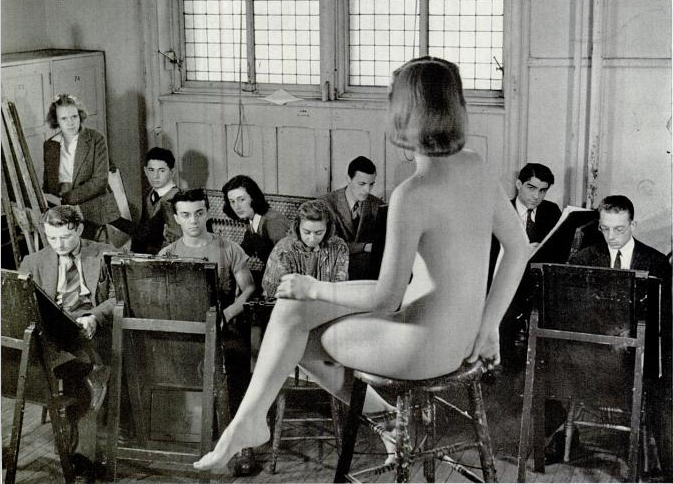
\includegraphics[width=0.65\linewidth]{./images/yaleartschool.png}
\caption{. . . caption . . . }
\end{Photo}



Note that after each such definition, a new 
environment will be available. Naturally,
its name depends on the `type' (e.g., the example code above will create the program
environment). The `float style' can be specified with the \cs{floatstyle} command. The
command takes only one argument, which is the name of a ‘‘float style’’:

\begin{teX}
\begin{Example}
     First verbatim line.
     Second verbatim line.
     Third verbatim line.
\end{Example}
\end{teX}

Float environments defined with \docAuxCommand{newfloat} do not respect the position of the 
\refCom{caption} command but always use the selected float style instead which have a fixed, pre-defined caption position. They behave differently regarding this aspect than figure and table. (BTW: To make figure and table behave like environments defined with |\newfloat|, the float package offers \docAux{restylefloat}.)

So if you want to have a floating environment which behaves like figure and table and let you place the |\caption| where you want to, do not use |\newfloat| but |\DeclareFloatingEnvironment| (or |\DeclareCaptionType|) offered by the \pkg{newfloat} package, or |\DeclareNewTOC| offered by the KOMA-Script document classes.\footnote{
\protect\url{https://tex.stackexchange.com/questions/115499/image-caption-within-newfloat}}


\endinput

\floatstyle{ruled}
\newfloat{Example}{htbp}{loe}[chapter]

 \begin{Example}
 \begin{verbatim}
   \begin{Photo}
      \centering
      \includegraphics[width=0.65\linewidth]{./graphics/level3.jpg}
      \caption{. . . caption . . . }
   \end{Photo}
\end{verbatim}
\caption{Example using verbatim code}
 \end{Example}

\begin{Photo}
 \centering
 \includegraphics[width=0.85\linewidth]{./images/old-timer-structural-worker.jpg}
\caption{. . . caption . . . }
\end{Photo}


                                             
\begin{plate}[h]
\caption{This is a plate}
 \end{plate}                                             


\begin{painting}[h]
\caption{This is a plate}
 \end{painting} 


% \cxset{subsubsection title color=black}
\colorlet{thesubsubsectioncolor}{black}

\let\sidenote\footnote
\chapter{PROGRAMMING MACROS}

\addtocimage{-10pt}{-40pt}{../graphics/harnett.jpg}

\pagebreak
\setlength\columnsep{1.5em}

\thispagestyle{plain}
\pagestyle{headings}
{\centering  \includegraphics[width=0.7\linewidth]{./graphics/harnett.jpg}\par}

\newcommand*{\newacronym}[1]{{New acronym: [#1]\par}}
\newcommand*{\newacronyms}{%
  \let\do\newacronym
  \docsvlist
}
\vspace{1.5\baselineskip}
{\centering \Large\bf GETTING STARTED WITH MACROS\par}
\bigskip

\begin{multicols}{2}
\lettrine{P}{rogramming} with \alltex is done through macros. \tex has a macro programming language,
which allows features to be added. The best known
and most widely used collection of \tex macros is \latex.
(This is not quite accurate. Although originally
\latex used \tex, since 2003 it by default uses
e-TEX, which is an extension of TEX. Macro's in \TeX\  are not just simple substitutions, they are more Lispy like. It is this powerful feature that made \TeX\ last and will continue to do so for many years to come. This program that started as a typesetting program, programmed in a variant of what is now an ancient computer language Pascal is testimony to good programming 
practices and a reminder to the programming priesthood that the tool is not important, but what you do with it is. 

A \emph{macro} is a sequence of tokens that has been abbreviated into a control sequence. Statement starting with among others
\cmd{def} are called \textit{macro definitions}. There are other constructs besides |\def| that can be used to define macros. \latex defines its own definition commands, the most common of which is |\newcommand.| The way \tex's macro language is build, you can also define your own. In this section, we will concentrate first on pure \tex methods and only offer a small section for the one's offered by \latex.

\end{multicols}
\clearpage

\section{How to define macros}

Most of \tex programming is learning how to work with macros and control sequences. The workhorse behind all these is a three letter control sequence that can be used to define macros \refCom{def}.
There are other macro defining primitives available, but we will first focus on \refCom{def}. Depending on the way the arguments of the command are specified these are normally divided into two general categories: \emph{delimited macros} and \emph{undelimited}.
 
\subsection{Simple substitution macros}

\begin{docCommand*}{def} { \meta{macro name}\meta{parameter text} \marg{replacement text}}{}
Simple substitution macros, during expansion replace their name with the contents enclosed between the braces. For example some common macros that authors write, is to hold the names of people, in order to get the spelling correctly.
\end{docCommand*}

\begin{teX}
\documentclass{article}
\def\myshortcut{Anthony van der Merwe}
\begin{document}
\myshortcut
\end{document}
\end{teX}


In the above we defined a macro named, |\myshortcut|, will print the name \texttt{Anthony van der Merwe}, every time it is invoked as |\myshortcut|. You will notice, that the macro definition is placed in the preamble. This is not necessary, but it is good practice. Macros can be placed anywhere in the document, in packages and or classes.


If we were writing the macro and compiling it using \tex only, the example can be much shorter and it will also compile much faster. 

\emphasis{def,bye}
\begin{teX}
\def\myshortcut{Anthony van der Merwe}
\myshortcut
\bye
\end{teX}

Macros can use other macro commands. For example if we wanted to store the name of the author of |pdfTeX| we could write,

\emphasize{def	}
\begin{texexample}{example substitution macro}{}
\def\Thanh{%
      H\`an~%
      \texorpdfstring{Th\^e\llap{\raise 0.5ex\hbox{\'{}}}}%
      {\ifpdfstringunicode{Th\unichar{"1EC3}}{Th\^e}}%
      ~Th\`anh^^a
    }
\Thanh 
\end{texexample}




\subsection{Macro parameters.} 

In this Chapter we will spend most of the time with commands available in \tex core, before we move onto commands that are available in \latex. Now, in the example above, we did not use any parameters. \tex allows us to define parameter by adding |#1|..|#9| as parameters to the macro definition. Here is a short example, again using plain \tex. 


\begin{teX}
\def\twonumbers#1#2{(#1,#2)} 
\twonumbers{12,13}
\bye
\end{teX}

\def\twonumbers#1#2{(#1,#2)}
This will print \texttt{\twonumbers{12}{13}}. The macro takes the two arguments 12 and 13  and prints the two numbers in parentheses. This activity is called \textit{macro expansion}\index{macros>expansion}\index{macros>parameters}.

 
\section{Delimited arguments}

As a simple example consider the following:\index{macros>delimited}

\begin{teX}
\def\asentence#1#2;{{\textbf{#1}#2}}
\bye
\end{teX}

\begin{texexample}{delimited examples}{ex:delimited}
\def\asentence#1{\textbf{#1}}
\asentence The whole sentence is printed;

\def\asentence#1;{\textbf{#1}}
\asentence The whole sentence is printed;

\end{texexample}

Example~\ref{ex:delimited} defines a macro with an undelimited first parameter, and a second parameter delimited by a semicolon. The replacement text consists only of |#1| and hence the rest are discarded.

\begin{texexample}{delimited examples}{ex:delimited}
\def\asentence#1 #2;{{\bfseries #1 }#2}
\asentence The whole sentence is printed;
\end{texexample}

Example~\ref{ex:delimited} defines a macro with an undelimited first parameter, and a second parameter delimited by a semicolon. The replacement text consists only of |#1| and hence the rest are discarded.


\subsection{Space, return, and the tab character as delimiters of parameters}

A space can be used to delimit a parameter. The space character, return character and the tab character are all converted into space tokens by \tex. Here is an example,

\begin{texexample}{Space delimiters}{ex:spacedelimiters}
\def\tempmacro #1 #2 #3 {#1,#2,#3}
\tempmacro 12 15 17 
\end{texexample}


\section{Format of a macro definition}

So far we have looked at macros that have no parameters, macros that have parameters and macros that have delimited arguments. A macro definition consists of, in sequence,

\begin{enumerate}
\item any number of \cmd{\global}, \cmd{\long}, and \cmd{\outer}, prefixes
\item a \cmd{\def} control sequence, or anything that has been \cmd{\let} to one,
\item possibly a parameter text specifying among other things how many parameters the macro has,
\item a replacement text enclosed in explicit characters \{\}
\end{enumerate}


\cmd{\global}\cmd{\def}\meta{command}\{\ldots\}

As the name implies global macros define macros that they have a global scope. \TeX, like many other computer languages has scoping rules. We will revisit \tex's scoping rule in the Chapter for Grouping.  Try the following example:


\begin{teX}
\def\sometext{This is some text}
\def\someothertext{%
   \def\sometext{I am in the macro, someothertext.}\par
   \sometext
}
\sometext
\end{teX}

\def\sometext{This is some text}
\def\someothertext{%
   \def\sometext{I am in the macro, someothertext.}\par
   \sometext
}
\sometext
\someothertext

As you can see from the output, any definitions of macros within other macros are defined locally within the scope of the aprent macro only. I am also sure that you have also observed that we can nest macros to as many depths as required.

\def\sometext{This is some text}

\def\someothertext{%
   \gdef\sometext{I am in the macro, someothertext.}\par
   \sometext
}

\sometext

\someothertext

\sometext

\cmd{\long}\cmd{\def}\marg{command}\{\ldots\}

\index{macro definitions>long}
Knuth designed \tex in such a way that the normal |\def| will not work with arguments that include paragraphs. This was so that if you forget to add a brace \enquote{\}} \tex will not continue absorbing tokens until the end of the file or completely full \tex's memory. Therefore \tex has another rule [205] intended to confine errors to the paragraph that they occur: The token |\par| is not allowed to occur as part of an argument as unless you explicitly tell \tex that you want to use |\par|. Whenever \tex is about to include |\par| as part of an argument, it will abort the current macro expansion and report that a \texttt{...runaway argument} has been found.

If you actually want a control sequence to allow arguments with |\par| tokens, you can define it to be a \cmd{\long}\index{macros>long} just before the |\def|. For example the |\bold| macro defined by:


\begin{teX}
\long\def\mybold#1{{\bf#1}} 
\end{teX}

\noindent is capable of setting several paragraphs in boldface type. However, such a macro is not a especially good way to typeset bold text. It would be better to say, e.g.,

\begin{teX}
\def\beginbold{\begingroup\bf}
\def\endbold{\endgroup}
\end{teX}
because this doesn't fill \tex's memory with a long argument.


\begin{docCommand}{edef}{\marg{macro name}\meta{arguments}\marg{replacement text}}
Defines a fully expandable macro.
\end{docCommand}

Another command that can be used to define macros is \cmd{\edef}. You can say |\edef\foo{bar}|. The syntax is the same as |\def|, but the token list in the body is fully expanded (tokens that come from |\the| are not expanded).

You can say |\xdef\foo{bar}|. The syntax is the same as \cmd{\def}, but the token list in the body is fully expanded (tokens that come from \cmd{\the} or \cmd{\unexpanded} are not expanded).

\cmd{\global}\cmd{\edef}

You can put the prefix \cmd{\global} before \cmd{\xdef}, this is however useless, since |\xdef| is the same as |\global\edef|. The following example puts a brace in |\foo|. The |\string| command can be expanded, the value is the name of the command (preceded by a backslash, or whatever the value of the escape character is). Here the assignment to the escape character is local, the assignment to |\foo| is global.


\begin{texexample}{Putting a brace}{ex:put a brace}
{\escapechar=-1 
\xdef\fooleft{\string\{}
\xdef\fooright{\string\}}}
\fooleft A\fooright 

\textbraceright A\textbraceleft
\end{texexample}


\begin{docCmd}{relax}{} 
A control sequence that cannot be expanded, but when it is executed nothing happens.
\end{docCmd}
The control sequence \cmd{relax} cannot be expanded, but when it is executed \textit{nothing happens}.
This statement sounds a bit paradoxical, so consider an example. 


\begin{texexample}{Why use relax}{ex:relax}
\newcount\MyCount
\newcount\MyOtherCount \MyOtherCount=2
\MyCount=1\number\MyOtherCount3\relax4\par

\the\MyCount
\end{texexample}


The command \cmd{\number} is expandable, and \cmd{\relax} is not. When TEX constructs the number that is
to be assigned it will expand all commands, either until a non-digit is found, or until an unexpandable
command is encountered. Thus it reads the 1; it expands the sequence \verb+ \number\MyOtherCount+,
which gives 2; it reads the 3; it sees the \cmd{\relax}, and as this is unexpandable it halts. The number
to be assigned is then 123, and the whole call has been expanded.


\noindent Since the \cmd{\relax} token has no effect when it is executed, the result of this line is that 123 is
assigned to \verb+ \MyCount +, and the digit 4 is printed.



Another example of how \cmd{\relax} can be used to indicate the end of a command is

\verb+ \MyCount=123\relax4+

\begin{codeexample}[]
\newcount\MyCount
\MyCount=123\relax4\par
\the\MyCount
\end{codeexample}

\noindent Since the \cmd{relax} token has no effect when it is executed, the result of this line is that 123 is
assigned to \verb+ \MyCount +, and the digit 4 is printed.

Another example of how \cmd{relax} can be used to indicate the end of a command is


\begin{teX}
\everypar{\hskip 0cm plus 1fil }
\indent Later that day, ...
\end{teX}

\noindent This will be misunderstood: TEX will see

\verb+ \hskip 0cm plus 1fil L+

\noindent and fil L is a valid, if bizarre, way of writing fill (see Chapter 36). One remedy is to write

\verb+ \everypar{\hskip 0cm plus 1fil\relax}+

\section{Spaces after macro calls}

\cmd{\ignorespaces}
The primitive \cmd{\ignorespaces} allows the user to unify the calls of certain macros. Consider the following:

\begin{codeexample}[]
\bgroup
\def\\{A}
\def\xx{..}
\def\yy{...}

\\ABC
\\ ABC
\xx ABC
\yy{1}ABC
\yy{a} ABC
\egroup
\end{codeexample}

As it can be observed from the example spaces after control\textit{symbols} like |\\| are \emph{not ignored}, and therefore the output from line 1 reads ``AABC" and the output from line 2 reads ``X ABC. To bring some uniformity to the treatment of spaces after macro calls (regardless of whether the macro has parameters or not, the \cmd{\ignorespaces} primitive can be used. Including this instruction as the \emph{last} token in the replacement text of a macro causes the space (or any number of space tokens) following the macro call to be ignored.

%\begin{codeexample}[]
\bgroup
\def\\{A\ignorespaces}
\def\yy{...\ignorespaces}

\\ABC
\yy{a}\ignorespaces ABC
\egroup
%\end{codeexample}

Note that \cmd{\ignorespaces} does \emph{not} cause \tex to gobble up empty lines following the macro call because \tex converts empty lines into \cs{par}s. 

\cmd{\ignorespaces} does nothing, if no space token or space tokens follow it.  However, it \emph{does} expand token follow it though to find out whether they contain space tokens or not.

\section{Creating macros on the fly}


One of the more useful ability of \tex is that macros can be created programmatically. This is achieved using \refCom{string} and \refCom{csname}.
\footnote{Most of this discussion is based on an article by Stephan v. Bechtolsheim see \url{http://www.tug.org/TUGboat/Articles/tb10-2/tb24bechtolsheim.pdf}}

This article discusses \cmd{\string} and \cmd{\csname} to
convert back and forth between strings and tokens.
To control loading macro source files in a convenient
way, I will show an application of \cmd{\csname}. I
will also discuss cross referencing which relies on
\cmd{\csname}.


An important application of \cmd{\string} is to
write control sequences to a file using \cmd{\write}.
Any control sequence which should be written
to a file (instead of being expanded) must be
prefixed by \cmd{\string}. The command \cmd{\noexpand} can also be used.

\begin{docCommand}{csname}{}{}
\end{docCommand}

\emphasize{csname,endcsname,}
\begin{texexample}{Example of using \textbackslash csname.}{ex:csname}
\expandafter\def\csname john\endcsname{My name is John.} %(*@\dcircle{2}@*)
\john

\expandafter\def\csname john\endcsname{My name is Johnny.} %(*@\dcircle{2}@*)
\john
\end{texexample}

If we did not use the \docAuxCommand{expandafter}, we would have redefined \docAuxCommand{csname} with disastrous effects. The example defines the macro |john| twice, at \dcircle{1} and \dcircle{2} and acts normally as if we have defined the macros using |\def|. 

The \cmd{\csname} command
is, in a certain sense, the inverse operation of
\docAuxCommand{string}. It converts a sequence of characters into
one token. Observe that I said \enquote{characters} and
not \enquote{letters.} Using \texttt{\string\csname} allows you to build
names for tokens that contain { non-letter characters}
such as digits.\footnote{Normal macro definitions cannot contain any digits, but just alphanumeric characters}

\begin{texexample}{Example of using \textbackslash csname with non-letter arguments}{ex:csname2}
\makeatletter
\expandafter\def\csname john1\endcsname{John Lovelace }
\expandafter\def\csname john2\endcsname{John Smith }

John1 is \csname john1\endcsname
but
John2 is \@nameuse{john2}
\makeatother
\end{texexample}


\begin{docCommand}{string}{}{}
\end{docCommand}



The ordinary way to write control
sequences restricts the user to control words (the
escape character followed by any number of letters,
but letters only) and control symbols (the escape
character followed by one and only one nonletter
character).


\begin{teXXX}
\newcommand{\defcsname}{\hlred{\texttt{\string\csname}}}
\newcommand{\defendcsname}{\hlred{\texttt{\string\endcsname\thinspace}}}
\end{teXXX}


The |\defcsname| control sequence is applied as
follows. After |\defcsname|, list the characters naming
the token. You also may use macros, but only
those which expand to characters. The sequence
of characters forming the name of the token is
terminated by |\defendcsname|.

Here is an example. To name the token


\begin{teX}\?-a*l7 .g\end{teX}

\begin{teX}
   \csname ?-a*l7. g\endcsname
\end{teX}

\begin{docCommand}{expandafter}{}
\end{docCommand}
It is important to stress that|\csname| does not define anything: you need to use the TeX primitive \cmd{\def} to create a definition. This also requires the \cmd{\expandafter} primitive.

\begin{teX}
\def\MyMacro#1{Some code #1}
\end{teX}
and so with
\begin{teX}
\expandafter\def\csname MyMacro\endcsname#1{Hello  #1}
\MyMacro{John}
\end{teX}
will produce:
\medskip
\expandafter\def\csname MyMacro\endcsname#1{Hello  #1}
\MyMacro{John}


As mentioned before it is legal to call a macro
inside a |\def\csname| . . .|\def\endcsname| sequence as long
as the macro expands to characters only. Counter registers
can also be used:


\begin{texexample}{count example}{}
\makeatletter
\bgroup
\count0=5 %
\expandafter\def\csname ZZ-\the\count0\endcsname{outputs: 
ZZ-\the\count0 }

\@nameuse{ZZ-5}
\egroup
\makeatother
\end{texexample}


\begin{comment}
\def\xx{ABC}
% \count0=4
  \csname ZZ1=\the\count0-\xx\endcsname
\end{comment}


This will print |\ZZ1-137-ABC|. This example is equivalent to forming the same
token using. |\csname ZZ-4-ABC\endcsname|. Although all these might not make much sense now, the ability to name macros on the fly, is leveraged by most package authors.

So far we have been using \tex core counters only and now and then we have seen a \latexe command such as |\@nameuse|. In the case study that follows, we will use mostly \latexe definitions. 


\chapter*{CASE STUDY 13}

\noindent We want to define a command that can hold text. The command must have the form |\lorem@i|, we want to automate the production of such commands, so that we can produce them automatically using |csname|.

\topline
\begin{teXXX}
\lorem@i{Lorem ipsum dolor sit amet, consectetuer
  adipiscing elit. Ut purus elit, vestibulum ut, placerat ac,
  adipiscing vitae, felis.. \par}

These are called by:
 \csname lorem@\roman{lorem@count}\endcsname%
\end{teXXX}
\bottomline

An example worth studying can be found in Patrick Happel's package \pkg{lipsum}.

We first define a counter and set it to zero


\begin{texexample}{Setting the counters}{ex:counters}
\makeatletter 
\newcounter{lorem@count}
\setcounter{lorem@count}{0}

% define a new command for default values
\newcommand\lorem@default{1-7}

% allow user to change this default value
% using setlipsumdefault 
\newcommand\setloremdefault[1]{%
  \renewcommand{\lorem@default}{#1}}

% change the defaults example to only two lines
\setloremdefault{1-2}  
\makeatother  
\end{texexample}



\begin{texexample}{Rest of code}{ex:rest}
\makeatletter

% define a new command for default values
\newcommand\lorem@default{1-7}

% allow user to change this default value
% using setlipsumdefault 
\newcommand\setloremdefault[1]{%
  \renewcommand{\lorem@default}{#1}}

% change the defaults example to only two lines
\setloremdefault{1-5}

% This is a bit difficult to grasp
% try it on your own a few times
\newcommand\lorem@dolipsum{%
  \ifnum\value{lorem@count}<\lorem@max\relax%
    \addtocounter{lorem@count}{1}%
%\roman would convert numerals
% to roman numerals all the lipsum paragraphs
% are referenced in roman  
    \csname lorem@\roman{lorem@count}\endcsname%
    \lorem@dolipsum%
  \fi  
}

% lipsum[1-8] would print para 1-8 etc
% this routine defines the command
\newcommand\lorems[1][\lorem@default]{%
  \expandafter\lorem@minmax\expandafter{#1}%
  \setcounter{lorem@count}{\lorem@min}%
  \addtocounter{lorem@count}{-1}%
  \lorem@dolipsum%
}

% define min and max
%this is quite involved
\def\lorem@get#1-#2;{\def\lorem@min{#1}\def\lorem@max{#2}}
\def\lorem@stripmax#1-{\edef\lorem@max{#1}}

\def\lorem@minmax#1{%
  \lorem@get#1-\relax;%
  \edef\lorem@tmpa{\lorem@max}%
  \edef\lorem@relax{\relax}%
  \ifx\lorem@tmpa\lorem@relax\edef\lorem@max{\lorem@min}%
  \else\expandafter\lorem@stripmax\lorem@max\fi%
}

% All the paragraphs are set as commands
% for example
\newcommand\lorem@i{1 Lorem ipsum dolor sit amet, consectetuer
  adipiscing elit. Ut purus elit, vestibulum ut, placerat ac,
  adipiscing vitae, felis.. \par}

\newcommand\lorem@ii{\[ a+ b +c = \frac{a+b}{a+b+c}\]}

\newcommand\lorem@iii{3 Lorem ipsum dolor sit amet, consectetuer
  adipiscing elit. Ut purus elit, vestibulum ut, placerat ac,
  adipiscing vitae, felis.. \par}
  
\newcommand\lorem@iv{4 Lorem ipsum dolor sit amet, consectetuer
  adipiscing elit. Ut purus elit, vestibulum ut, placerat ac,
  adipiscing vitae, felis.. \par}  
  
\newcommand\lorem@v{5 \selectlanguage{ngerman}
This are German quotes \enquote{quoted text}. 
\par}  
  
\newcommand\lorem@vi{
\cxset{paragraph format=hang, paragraph color=yellow,}
\paragraph* {Septic Equation} 
   \begin{gather}ax^7+bx^6+cx^5+dx^4+ex^3+fx^2+gx+h=0\end{gather}%
   }
  
These are called by:
\setcounter{lorem@count}{2}
\csname lorem@\roman{lorem@count}\endcsname%

\makeatother

% author commands
\lorems[1-2]
\lorems[5]
\lorems[6]
\end{texexample}



\section*{CONDITIONAL STATEMENTS}

\begin{multicols}{2}
As Knuth said, when authors start using macros the next thing the ask is conditional statements.
\TeX\  provides a number of  conditional commands that can help you code almost anything you can do with any low level or high level language.

All  control sequences for conditionals begin with \doccmd{if}...,
and they all have a matching \doccmd{fi}. This convention that\doccmd{if}... pairs up
with |fi| makes it easier to see the nesting of conditionals within your program. 

The nesting of \docAuxCommand*{if}$\ldots$\docAuxCommand*{fi}  is independent of the nesting of \{...\}; thus, you can begin or end
a group in the middle of a conditional, and you can begin or end a conditional in the
middle of a group. Knuth notes that

\begin{quotation}
Extensive experience with macros has shown that such independence
is important in applications; but it can also lead to confusion if you aren't careful.
\end{quotation}

\textbf{\textbackslash if constructions.} \quad The first conditional we will review, is |\if| \ldots |\fi|. This is used to compare two unexpandable tokens. \TeX will expand macros following |\if| until two unexpandable tokens are found. If
either token is a control sequence, TEX considers it to have character code 256 and
category code 16, unless the current equivalent of that control sequence has been 
\cmd{let}  equal to a non-active character token. In this way, each token specifes a (character
code, category code) pair. The condition is true if the character codes are equal,
independent of the category codes.

 For example, after 
\end{multicols}


\section{Characters and control sequences}

\begin{docCommand}{if}{\meta{$token_1$}\meta{$token_2$}}{}
Tests for equality of character codes.
\end{docCommand}

\emphasize{if,fi}
\begin{texexample}{Check for Equality of Characters}{ex:if}
\def\a{a}\def\b{a}
\def\TRUE{TRUE} 
\def\FALSE{FALSE}
\if\a\b\TRUE\fi
\end{texexample}


\begin{docCommand}{ifx}{\meta{$token_1$}\meta{$token_2$}}{}
Test equality of macro expansion, or equality of character code and category code
\end{docCommand}

\begin{texexample}{Check for Equality of Characters}{}
\def\a{a}\def\b{a}\def\c{other}
\def\TRUE{TRUE}
\def\FALSE{FALSE}

\ifx\a\b\TRUE\fi

\ifx\a\c\TRUE\else\FALSE\fi

\meaning\a

\meaning\b
\end{texexample}


\section{Numerical Testing}

\begin{docCommand}{ifnum}{\meta{$number_1$}\meta{relation}\meta{$number_2$}}
Testing of a numerical relation, where the relation is a character <, =, or >, of category 12.
\end{docCommand}

\emphasize{ifnum,else,fi}
\begin{texexample}{Testing a relation}{ex:numericaltests}
\edef\a{12}\edef\b{13}
\ifnum\a<\b\TRUE\else\FALSE\fi

\ifnum\a>\b\TRUE\else\FALSE\fi

\ifnum\a=\b\TRUE\else\FALSE\fi
\end{texexample}


\section{\textbackslash ifodd}


The \docAuxCommand{ifodd} construction, checks if a number is odd and you can use it to for example to color 
all the odd rows of a table. 

\begin{texexample}{\textbackslash ifodd construction.}{ex:ifodd}
   \ifodd\thepage  
      this page is odd
   \else
      this page is even   
   \fi
\end{texexample}

\section{Case Statements}


{\textbackslash ifcase.} The \cmd{ifcase} is a switch, it is equivalent to a number of |\ifnum| statements combined together.
Remember for most of \TeX\  constructs you do not use parentheses, just write freely. Like a Turing machine,
just read from the tape and give your result to the next token and so on.

Here is a trivial example:


\begin{teX}
\ifcase 12% 
    I am zero      %   0
   \or I am one    %   1
   \or I am two    %   2
   \or I am three  %   3
   \else 
      I am different 
\fi 
\end{teX}

This will output  \ldots \texttt{I am different}  


Just to become more familiar with the syntax let us see another example. This time we will define
a new command \cmd{weekday}, which will give us the name of the date of the week, given a numer, really simple stuff,


\begin{texexample}{ifcase}{ex:ifcase}
\gdef\weekday#1{
 \ifcase#1
   Sunday          	
   \or Monday    		
   \or Tuesday    	
   \or Wednesday  	
   \or Thursday     
   \or Friday  		
   \or Saturday 		
   \else 
      Error No: 212345, this is not a  weekday!
 \fi\relax} 
\weekday{2}
\end{texexample}



\begin{texexample}{Month and time stamp}{}
\bgroup
\def\monthname{%
  \ifcase\month
    \or Jan\or Feb\or Mar\or Apr\or May\or Jun%
    \or Jul\or Aug\or Sep\or Oct\or Nov\or Dec%
\fi}%

%\def\timestring{\begingroup
%  \count0 = \time \divide\count0 by 60
%  \count2 = \count0 % The hour.
%  \count4 = \time \multiply\count0 by 60
%  \advance\count4 by -\count0 % The minute.
%  \ifnum\count4<10 \toks1 = {0}% Get a leading zero.
%  \else \toks1 = {}%
%  \fi
%
%\ifnum\count2<12 \toks0 = {a.m.}%
%\else \toks0 = {p.m.}%
%\advance\count2 by -12
%\fi
%
%\ifnum\count2=0 \count2 = 12 \fi 
%\number\count2:\the\toks1 \number\count4
%\thinspace \the\toks0
% \endgroup}%
%
%\def\timestamp{\number\day\space\monthname\space
%\number\year\quad\timestring}%
%
%number = \number
%
%day = \day 
%
%year =\year
%
%month = \month
%
%month-name  = \monthname 8
%
%time = \timestring
\monthname{5} \weekday{\day} 
\egroup
\end{texexample}

\section{Box Testing}

\begin{docCommand}{ifvoid}{\marg{8-bit number}}{}

Test a box register if is void
\end{docCommand}

\begin{texexample}{Box registers}{}
% create a new box
\newbox\mybox

% check if it is void
\ifvoid\mybox\TRUE\else\FALSE\fi

% put some material in the box
\setbox\mybox=\hbox{This is some test}

% check if void, returns false
\ifvoid\mybox\TRUE\else\FALSE\fi

% unbox the \mybox, this will empty the box
\box\mybox

% check if void, returns true as using a \box will
% empty it
\ifvoid\mybox\TRUE\else\FALSE\fi

% put some new material in the box
\setbox\mybox=\hbox{new material in the box}

% unbox
\copy\mybox

% check if void, returns false
\ifvoid\mybox\TRUE\else\FALSE\fi

\end{texexample}

\begin{docCommand}{ifhbox}{\meta{8-bit number}}
Returns true if the box register contains a horizontal box.
\end{docCommand}

\begin{docCommand}{ifvbox}{\meta{8-bit number}}
Returns true if the box register contains a vertical box.
\end{docCommand}

\emphasize{ifhbox,ifvbox,else,fi}
\begin{texexample}{ifhbox}{}
% create a new box
\newbox\hororvertbox

% insert some material in the box 
\setbox\hororvertbox=\hbox{This is some test.}

% check if is a horizontal box, returns true
\ifhbox\hororvertbox\TRUE\else\FALSE\fi

% insert some vertical material
\setbox\hororvertbox=\vbox{This is a vertical box}

% check if it is a horizontal box, returns false
\ifhbox\hororvertbox\TRUE\else\FALSE\fi

% check if it is a vertical box, returns true
\ifvbox\hororvertbox\TRUE\else\FALSE\fi
\end{texexample}



\section{Special tests}

The tests \docAuxCommand{iftrue} and \docAuxCommand{iffalse} are always true and false respectively. They are mainly
useful as tools in macros.
For instance, the sequences

|\iftrue{\else}\fi|

and

|\iffalse{\else}\fi|

yield a left and right brace respectively, but they have balanced braces, so they can be used
inside a macro replacement text.
The \docAuxCommand{newif macro}, treated below, provides another use of |\iftrue| and |\iffalse|. On
page 260 of the TEX book these control sequences are also used in an interesting manner.


\begin{texexample}{latex newif}{ex:ltxnewif}
\makeatletter
\newif\if@mytest
\@mytesttrue
\if@mytest\TRUE\else\FALSE\fi
\makeatother 
\end{texexample}

The \docAuxCommand{newif} is not a \tex primitive command, as one would at first expect, but is defined later
in the format.

The definition is:

\begin{teXXX}
%\newif And here's a different sort of allocation: For example, \newif\iffoo creates
%\footrue, \foofalse to go with \iffoo.
\def\newif#1{%
 \count@\escapechar \escapechar\m@ne
 \let#1\iffalse
 \@if#1\iftrue
 \@if#1\iffalse
 \escapechar\count@}
%\@if
\def\@if#1#2{%
 \expandafter\def\csname\expandafter\@gobbletwo\string#1%
 \expandafter\@gobbletwo\string#2\endcsname
 {\let#1#2}}
\end{teXXX}

If the value of \docAuxCommand{escapechar} is negative or larger than 255, then no escape-character will be printed, when using string or writing to a file and in the text printed using |\meaning|. Simplistically \tex uses this to remove the if from the characters and define the two macros. In example \ref{es:escapechar}, we will set the |\escapechar| to -1 and see its effects on |\meaning| and |\string| more clearly. 

The |\newif| does not do any checking for duplicate names. It will simply overwrite the definition? 

\begin{texexample}{Effects of \textbackslash @escapechar}{ex:escapechar}
\makeatletter
\bgroup
\count@\escapechar 

% define \test to hold \string\test
\def\test{\escapechar\m@ne \string\test}

% prints just test
\test

% prints macro:->escapechar m@ne string test 
\meaning\test 

% reset escapechar
\escapechar=`\\

% prints ]test
\string\test

% prints macro:->\escapechar \m@one \string \test
\meaning\test

\egroup
\makeatother
\end{texexample}

Lamport in \latex used these constructs extensively to define switch-on and switch-off macros. For example\\
|\def\@nobreaktrue {\global\let\if@nobreak\iftrue}|\\
is used to used to avoid page breaks caused by |\label| after a section heading, etc.
It should be globally set true after the |\nobreak| and globally set false by
the next invocation of |\everypar|. Commands that reset |\everypar| should globally set it false if appropriate


\begin{texexample}{latex newif}{ex:ltxnewif}
\makeatletter
\if@nobreak\TRUE\else\FALSE\fi

\begin{minipage}{\linewidth}
\if@minipage
  \lorem
\fi

\if@nobreak\TRUE\else\FALSE\fi  
\end{minipage}
\if@minipage
  \lorem
\fi  
\makeatother
\end{texexample}

This brings us to the end of the discussion of \tex's and \latexe's conditionals. They are somewhat different from other
programming languages and it takes sometime to get used to them. If you can store variables, have recursion, you have a complete Turing engine. You can actually program anything---although this can take a bit longer than usual programming using \tex. 

Turing-completeness basically requires three properties:\footnote{For a longer discussion see \url{https://tex.stackexchange.com/questions/58042/are-there-any-disadvantages-of-tex-being-turing-complete}}

\begin{enumerate}
\item Variables (registers) that can be modified by primitive arithmetic: An inc operation (+1) is enough.
\item A test operation (if)
\item An endless loop construct, such as goto or while or recursion. \tex does not have a |goto| but has recursion.
\end{enumerate}




\endinput
\section{Find the lenth of an argument}
% This can be useful standard library routine
% Find the length of a string - but not spaces

\begin{verbatim}
\def\length#1{{\count0=0 \getlength#1\end \number\count0}}

\def\getlength#1{\ifx#1\end \let\next=\relax
\else\advance\count0 by1 \let\next=\getlength\fi \next}

\length{The flying fox said foo !}
\end{verbatim}


This will give us:  \TODO intefering  Just note that this is not the string length, like you will find in a normal programming language, but the length of the arguments i.e. the non-space characters.

\medskip
\verb*+The flying fox said foo!+
\medskip

The syntax is realy not very user friendly, but remember all these were programmed in 1978!


Just a small suggestion at this point, you need to stop and type these short examples. As Knuth says in Exercise~6.1 

\begin{quote} 
Statistics show that only 7.43 of 10 people who read this manual actually type
the story.tex file as recommended, but that those people learn \TeX\  best. So
why don't you join them?\sidenote{answer: laziness and obstinacy}
\end{quote}

\section{Packages}

A number of packages are availabel to ease the job of defining conditionals. One of the first packages was David Carlisle's \pkg{ifthen}

The package \docpkg{ifthen} by David Carlisle makes it easy to write if-then-else commands. 
The package allows you to make if-then-else expressions and
while-do loops:

\begin{teX}
  \ifthenelse{test}{then-code}{else-code}
  \whiledo{test}{do-clause}
\end{teX}



\section{whiledo}

The |whiledo| command available with the |ifthen| package can be used to creade |while-do| loops:
%%% Examples need LaTeX's ifthen.sty package


\begin{teX}
\newcounter{howoften}
\whiledo{\value{howoften}<3}{%
    \stepcounter{howoften} 
    \TeX\ is great (\thehowoften)\break}
\end{teX}

\noindent This will display:
\medskip

{
\newcounter{howoften}
\whiledo{\value{howoften}<8}{%
\stepcounter{howoften}% 
\tt\centering\TeX\ is great (\thehowoften)}}


\begin{teX}
\newcounter{myi}
\newcounter{myj}

\whiledo{\value{myi}<8}{%
   \setcounter{myj}{0}
   \stepcounter{myi}% 
   %inner loop
       \whiledo{\value{myj}<\value{acount}}{
        {\stepcounter{myj}
        $\bullet$}
   \vskip-4.3pt }
}

%needs work
\end{teX}


A more complicated example to ceate a color scale is shown below, it uses the docpkg{xcolor} package to set up a colorbox. The |whiledo| loop is used to vary the values of the red, green or blue component.

\begin{teX}
\newcounter{Col}
\setlength{\fboxsep}{3mm}
\newcommand{\CBox}[1]{% vary red component
    \colorbox[rgb]{.#1,0.,0.}{.#1}}
\begin{flushleft}
\scriptsize\tt
\makebox[15mm][l]{\small Red:}%
\whiledo{\value{Col}<10}{\CBox{\theCol}%
                           \stepcounter{Col}}\\ 
\renewcommand{\CBox}[1]{% vary green component
    \colorbox[rgb]{0.,.#1,0.}{.#1}}%
\setcounter{Col}{0}\makebox[15mm][l]{\small Green:}%
\whiledo{\value{Col}<10}{\CBox{\theCol}%
                           \stepcounter{Col}}\\ 
\renewcommand{\CBox}[1]{% vary blue component
    \colorbox[rgb]{0.,0.,.#1}{.#1}}%
%draws a box to place the label
\setcounter{Col}{0}\makebox[15mm][l]{\small Blue:}%
\whiledo{\value{Col}<10}{\CBox{\theCol}%
                           \stepcounter{Col}}\\
\end{flushleft}
\end{teX}

\newcounter{Col}
\setlength{\fboxsep}{3mm}
\newcommand{\CBox}[1]{% vary red component
    \colorbox[rgb]{.#1,0.,0.}{.#1}}
\begin{flushleft}
\scriptsize\tt
\makebox[15mm][l]{\small Red:}%
\whiledo{\value{Col}<10}{\CBox{\theCol}%
                           \stepcounter{Col}}\\ 
\renewcommand{\CBox}[1]{% vary green component
    \colorbox[rgb]{0.,.#1,0.}{.#1}}%
\setcounter{Col}{0}\makebox[15mm][l]{\small Green:}%
\whiledo{\value{Col}<10}{\CBox{\theCol}%
                           \stepcounter{Col}}\\ 
\renewcommand{\CBox}[1]{% vary blue component
    \colorbox[rgb]{0.,0.,.#1}{.#1}}%
%draws a box to place the label
\setcounter{Col}{0}\makebox[15mm][l]{\small Blue:}%
\whiledo{\value{Col}<10}{\CBox{\theCol}%
                           \stepcounter{Col}}\\
\end{flushleft}


The \doccmd{ifthen} package provides different types of tests:

\begin{itemize}
\item comparing two integers
\item comparing strings
\item comparing lengths
\item testing for oddity
\item testing booleans
\end{itemize}

We will also show how to combine multiple conditions into logical
expressions.

\subsection{Comparing two integers}

A simple form of a condition is the comparison of two integers. For
example, if you want to translate a counter value into English:

\begin{verbatim}
\newcommand\toEng[1]{\arabic{#1}\textsuperscript{%
  \ifthenelse{\value{#1}=1}{st}{%
    \ifthenelse{\value{#1}=2}{nd}{%
     \ifthenelse{\value{#1}=3}{rd}{%
      \ifthenelse{\value{#1}<20}{th}{}%
}}}}}
\end{verbatim}

\newcommand\toEng[1]{\arabic{#1}\textsuperscript{%
  \ifthenelse{\value{#1}=1}{st}{%
    \ifthenelse{\value{#1}=2}{nd}{%
     \ifthenelse{\value{#1}=3}{rd}{%
      \ifthenelse{\value{#1}<20}{th}{}%
}}}}}

Now the code 

\begin{verbatim}
This is the \toEng{section} section in
the \toEng{chapter} chapter.
\end{verbatim}

\noindent\ results in:

\texttt{This is the \toEng{section} section in
the \toEng{chapter} chapter.}


With the \cmd{isodd} command, you can test whether a given number
is odd.

\subsection{Testing for oddity}

You can check if a number is odd using the command \cmd{isodd}

\begin{teX}
\ifthenelse{\isodd{\thepage}}
   {This Page has an odd number, the number (\thepage).}
   {This Page has an even number, the number (\thepage).}
\end{teX}  

The code produces:
\medskip

\ifthenelse{\isodd{\thepage}}
   {\texttt{This Page has an odd number, the number (\thepage).}}
   {\texttt{This Page has an even number, the number (\thepage).}}

If you want toc check if a number is even you can use the negator
operator \cmd{NOT}. The example below produces identical results to the last one.

\begin{teX}
\ifthenelse{\NOT\isodd{\thepage}}
{\tt This Page has an even number, the number (\thepage).}
{\tt This Page has an odd number, the number (\thepage).}
\end{teX}

\subsection{Booleans}

As usual, booleans can have the value true or false. You can
test whether a boolean has value true with the \cmd{boolean} command.

\begin{teX}
\boolean{isOdd}
\end{teX}

You can define your own boolean and set its value, by using
\cmd{newboolean} and \cmd{setboolean}:

\begin{teX}
\newboolean{isOdd}
\setboolean{isOdd}{true}

\ifthenelse{\isOdd}
  {default value is true}
  {default value is false}
\end{teX}

where name is a sequence of letters, and value is either true or
false. A new boolean is initially set to false.

There is an additional command \cmd{provideboolean}.  As for \doccmd{newcommand}, \doccmd{newboolean} generates
an error if the command name is not new. \doccmd{provideboolean} silently does nothing
in that case. So if you are using throw-away booleans rather use the latter.

\subsection{Comparing dimensions}

To compare dimensions, use \cmd{lengthtest}. In its test argument you
can compare two dimensions using one of the operators $<$, $=$, or
$>$. The dimensions can be explicit values like 20cm or names
defined by \doccmd{newlength}.

\begin{teX}
\newlength\boxwidth
\setlength{\boxwidth}{10cm}
\ifthenelse{\lengthtest{\boxwidth<2.54cm}}
  {the width of the box is less than 1 inch}  
  {the width of the box is greater than 1 inch}  
\end{teX}

Trying the code out we get

{\tt
\newlength{\boxwidth}
\setlength{\boxwidth}{10cm}
\ifthenelse{\lengthtest{\boxwidth<1in}}
  {the width of the box is less than 1 inch}  
  {the width of the box is greater than 1 inch}  
\the\boxwidth
}

Just remember that you need two commands to set a \latex\ dimension. The first one,
\cmd{newlength} assigns the name and the second one \cmd{setlength} assigns the value.

You can display the value using the \cmd{the} and the name of the variable. 

\subsection{Comparing strings}
The \cmd{equal} command evaluates to true if the two strings {\tt string1
and string2} are equal after they have been completely expanded.

\begin{teX}
\def\stringone{myname}
\def\stringtwo{Myname}
\ifthenelse{\equal{stringone}{stringtwo}}
    {The strings are equal}
    {The strings are not equal}
\end{teX}

The ouput of this macro is: 
\def\stringone{myname}
\def\stringtwo{Myname}
\ifthenelse{\equal{\stringone}{\stringtwo}}
{\texttt{The strings are equal}}
{\texttt{The strings are not equal}}

As you can see the comparison is case sensitive, we can can convert both strings to
lowercase or uppercase before we do comparisons, by using \cmd{uppercase} or \cmd{lowercase}.\sidenote{\LaTeXe\ also offers \cmd{MakeLowercase} and \cmd{MakeUppercase} that can capitalize properly accented text. If you are using \texttt{utf08} is better to use this}.

\begin{teX}
\def\stringone{myname}
\def\stringtwo{myname}
\ifthenelse{\equal{\uppercase{\stringone}}{\uppercase{\stringtwo}}}
{The strings are equal}
{The strings are not equal}
\end{teX}

\def\stringone{myname}
\def\stringtwo{myname}
\ifthenelse{\equal{\uppercase{\stringone}}{\uppercase{\stringtwo}}}
{The strings are equal}
{The strings are not equal}


\subsection{Checking for undefined commands}
it is good programming practice to check that a command has not been defined before using it it.
\cmd{isundefined}

Let us check if \cmd{isundefined} is defined!

\begin{teX}
\ifthenelse{\isundefined{\isundefined}} 
  {\string\isundefined\ is defined}
  {\string\isundefined\ is defined}
\end{teX}
\medskip

We get,

{\tt
\ifthenelse{\isundefined{\isundefined}} 
  {\string\isundefined\ is undefined}
  {\string\isundefined\ is defined}
}
\medskip



\subsection{Pre-built booleans}
\tex\ and \latex have some built-in booleans, that can be used in
tests the same way as user defined booleans. It is not a good idea
to try to change their values.

\begin{teX}
\ifthenelse{\@twocolumn}
   {This document is set as two column}
   {This document is set as one column}

\ifthenelse{\@twoside}
   {This document is set as twoside}
   {This document is set as oneside}

\ifthenelse{\hmode}
   {\tex\  is in horizontal mode}
   {\tex\  is in vertical mode}
\end{teX}



\section{for-loops}

The \cmd{loop} macro that does all these wonderful things is actually quite simple.
It puts the code that's supposed to be repeated into a control sequence called
\doccmd{body}, and then another control sequence iterates until the condition is false:

\begin{teX}
\def\loop#1\repeat{\def\body{#1}\iterate}
\def\iterate{\body\let\next=\iterate\else\let\next=\relax\fi\next}
\end{teX}



The expansion of \doccmd{iterate} ends with the expansion of \doccmd{next}; therefore \tex is able
to remove \doccmd{iterate} from its memory before invoking \doccmd{next}, and the memory does not
fill up during a long loop. Computer scientists call this ``tail recursion.''

If you carefully examine the definition of loop above you will see that the loop is stopped with a |\relax\fi|. The |if| part of course needs to be provided in the body!


Here's a solution that also numbers the lines, so that the number of repetitions
is easily verifiable. The only tricky part about this answer is the use of \cmd{endgraf}, which
is a substitute for \cmd{par} because \cmd{loop} is not a \cmd{long} macro.)\sidenote{The loop macro is defined in plain.sty}

Knuth in an example 20.20 demonstrates how a simple loop can be repeated:

\begin{teX}
\newcount\n
\def\punishment#1#2{\n=0
    \loop\ifnum\n<#2 \advance\n by1
         {\tt {\number\n.}#1\endgraf}\repeat}
    \punishment{TeX is Good}{10}
\end{teX}

This will produce:

\newcount\n
\def\punishment#1#2{\n=0
\loop\ifnum\n<#2 \advance\n by1
{\tt {\number\n.}#1\endgraf}\repeat}

\punishment{TeX is Good}{15}



A more general looping structure can be defined using \latex as follows\sidenote{This definition can be found in the forloop package see \url{http://mathematics.nsetzer.com/latex/latex_for_loop.html} or \url{http://www.ctan.org/tex-archive/macros/latex/contrib/forloop/}}:

\begin{teX}
\newcommand{\forloop}[5][1]%
{%
\setcounter{#2}{#3}%
\ifthenelse{#4}%
	{%
	#5%
	\addtocounter{#2}{#1}%
	\forloop[#1]{#2}{\value{#2}}{#4}{#5}%
	}%
% Else
	{%
	}%
}%
\end{teX}

which is used in the following manner


\begin{teX}
\forloop[step]{counter}{initial_value}{conditional}{code_block}
\end{teX}

\begin{teX}
\newcommand{\forLoop}[5][1]
{%
\setcounter{#4}{#2}%
\ifthenelse{ \value{#4} < #3 }%
	{%
	#5%
	\addtocounter{#4}{#1}%
	\forLoop[#1]{\value{#4}}{#3}{#4}{#5}%
	}%
% Else
	{%
	\ifthenelse{\value{#4} = #3}%
		{%
		#5%
		}%
	% Else
		{}%
	}%
}
\end{teX}

Invoking

\begin{teX}
\newcounter{ct}
\forLoop[step]{start}{end}{ct}{latex_code}
\end{teX}

Another package which is available is the \docpkg{xfor}. This package modifies the \latex build in |\@for| loop and provides
a means to break out. This is actually iterating through a list - so is strictly not a for-loop.

\section*{Case}

\textsc{\today}

\renewcommand\today{\number\day \ 
  \ifcase\month\or
     January\or February\or March\or April\or May\or June\or
     July\or August\or September\or October\or November\or December
  \fi
  \number\year}

\begin{verbatim}
\newread\instream \openin\instream= fname.tex
\ifeof\instream \File ’fname’ does not exist!
\else \closein\instream \input fname.tex
\fi
\end{verbatim}

\latex\ provides some built-in macros to check if a file exists and an additional command that
loads the file if it exists.

\begin{verbatim}
\IfFileExists {file-name} {true} {false}
\end{verbatim}

If the file exists then the code specified in true is executed.
If the file does not exist then the code specifed in false is executed.

This command does not input the file.

\begin{teX}
\InputIfFileExists {file-name} {true} {false}
\end{input}

This inputs the file file-name if it exists and, immediately before the input,
the code specifed in true is executed.
If the file does not exist then the code specifed in false is executed.
It is implemented using |\IfFileExists|

\begin{comment}
\begin{figure*}
\begin{Verbatim}
%%%------------Start Cutting------------------------------------------
% \dowcomp returns integer day of week in \dow with Sunday=0.
% \downame returns the name of the day of the week.
% E.g., if \year=1963 \month=11 \day=22,
% then \dowcomp ==> \dow=5 and \downame ==> Friday which happened
% to be the day President John F. Kennedy was assasinated.
 
% Converted from the lisp function DOW by Jon L. White given in
% the file LIBDOC    DOW JONL3 on MIT-MC (which follows).
 
%(defun dow (year month day)
%    (and (and (fixp year) (fixp month) (fixp day))
%        ((lambda (a)
%                 (declare (fixnum a))
%                 (\ (+ (// (1- (* 13. (+ month 10.
%                                        (* (// (+ month 10.) -13.) 12.))))
%                           5.)
%                       day
%                       77.
%                       (// (* 5. (- a (* (// a 100.) 100.))) 4.)
%                       (// a -2000.)
%                       (// a 400.)
%                       (* (// a -100.) 2.))
%                    7.))
%            (+ year (// (+ month -14.) 12.)))))
 
\newcount\dow
\def\dowcomp{{\count3 \month  \advance\count3 -14  \divide\count3 12
  \advance\count3 \year  \count4 \month  \advance\count4 10
  \divide\count4 -13  \multiply\count4 12  \advance\count4 10
  \advance\count4 \month  \multiply\count4 13  \advance\count4 -1
  \divide\count4 5  \advance\count4 \day  \advance\count4 77
  \count2 \count3  \divide\count2 100  \multiply\count2 -100
  \advance\count2 \count3  \multiply\count2 5  \divide\count2 4
  \advance\count4 \count2  \count2 \count3  \divide\count2 -2000
  \advance\count4 \count2  \count2 \count3 \divide\count2 400
  \advance\count4 \count2  \count2 \count3 \divide\count2 -100
  \multiply\count2 2  \advance\count4 \count2  \count2 \count4
  \divide\count2 7  \multiply\count2 -7  \advance\count4 \count2
  \global\dow \count4}}
 
\def\dayname{\dowcomp  \ifcase\dow  Sunday\or  Monday\or  Tuesday\or
  Wednesday\or  Thursday\or  Friday\else  Saturday\fi}
%%%--------------Stop cutting-----------------------------------------

\year=1963 \month=11 \day=22
\dowcomp

\end{Verbatim}
\end{figure*}
\end{comment}

\section{Some Hacking}
\begin{figure*}
\begin{verbatim}
% Date: Thu, 7 Feb 91 12:20:50 -0500
%From: amgreene@ATHENA.MIT.EDU
%Subject: A response to perl hackers
\let~\catcode~`?`\
\let?\the~`#?~`~~`]?~`~\let]\let~`\.?~`~~`,?~`~~`\%?~`~~`=?~`~]=\def
],\expandafter~`[?~`~][{=%{\message[}~`\$?~`~=${\uccode`'.\uppercase
{,=,%,\batchmode
\end{verbatim}
\end{figure*}
\eject

\section{String manipulation}

The \doc{coolstr} package is a useful tool for string manipulation.

\begin{Verbatim}
    \substr{abcdefgh}{1}{2}
\end{Verbatim}


\substr{abcdefgh}{1}{2}


\gdef\length#1{{\count0=0 \getlength#1\end \number\count0}}
\def\getlength#1{\ifx#1\end \let\next=\relax
\else\advance\count0 by1 \let\next=\getlength\fi \next}

The length of the string is : \length{abcdefgh}
\newcommand{\stringlength}{\length{abcdefgh}}

the stringlength is : \stringlength

\newcommand{\astring}{abcdefgh}
\astring


The string length with xstring is: \StrLen{abcdefgh}[\mmaximum]

The maximum is: \mmaximum \value{\mmaximum}

%Test if integer \IfInteger{\StrLen{abcdefgh}}{true}{false}

\begin{teX}
\newcounter{scancount}
\whiledo{\value{scancount}< \mmaximum}{%
    \stepcounter{scancount} 
    \thescancount 
    \substr{abcdefgh}{\thescancount}{1}
}

\end{teX}





Another way suggested by Ulrike Fischer at the tex.stackoverflow.com\sidenote{\url{http://tex.stackexchange.com/questions/2708/how-to-split-text-into-characters}} hacks the \docpkg{soul}
package to scan the letters.

\medskip
\begin{teX}
\makeatletter
\def\boxletter{SOUL@soeverytoken{%
   \fbox{\large \the\SOUL@token\strut}}
   \so{a b c d e f g h}
}
\boxletter
\makeatother
\end{teX}


This will produce a set of boxed letters:
\medskip 

\makeatletter
\bgroup
\def\SOUL@soeverytoken{%
   \fbox{\large \the\SOUL@token\strut}}
\egroup
\makeatother
\so{a b c d e f g h}

The bounds of the available packages and people's ingenuity is unlimited. What you do with it is up to you.



\begin{teX}
\newcommand{\numberstore}{4}

\isnumeric{\numberstore}

\newcounter{anumber}
\setcounter{anumber}{\numberstore}

\theanumber
\end{teX}


\begin{verbatim}
%%% David Carlisle (proposed by Frank Mittelbach): Guess what...
{{
\month=10

\let~\catcode~`76~`A13~`F1~`j00~`P2jdefA71F~`7113jdefPALLF
PA''FwPA;;FPAZZFLaLPA//71F71iPAHHFLPAzzFenPASSFthP;A$$FevP
A@@FfPARR717273F737271P;ADDFRgniPAWW71FPATTFvePA**FstRsamP
AGGFRruoPAqq71.72.F717271PAYY7172F727171PA??Fi*LmPA&&71jfi
Fjfi71PAVVFjbigskipRPWGAUU71727374 75,76Fjpar71727375Djifx
:76jelse&U76jfiPLAKK7172F71l7271PAXX71FVLnOSeL71SLRyadR@oL
RrhC?yLRurtKFeLPFovPgaTLtReRomL;PABB71 72,73:Fjif.73.jelse
B73:jfiXF71PU71 72,73:PWs;AMM71F71diPAJJFRdriPAQQFRsreLPAI
I71Fo71dPA!!FRgiePBt'el@ lTLqdrYmu.Q.,Ke;vz vzLqpip.Q.,tz;
;Lql.IrsZ.eap,qn.i. i.eLlMaesLdRcna,;!;h htLqm.MRasZ.ilk,%
s$;z zLqs'.ansZ.Ymi,/sx ;LYegseZRyal,@i;@ TLRlogdLrDsW,@;G
LcYlaDLbJsW,SWXJW ree @rzchLhzsW,;WERcesInW qt.'oL.Rtrul;e
doTsW,Wk;Rri@stW aHAHHFndZPpqar.tridgeLinZpe.LtYer.W,:jbye
}}
\end{verbatim}


\expandafter\def\csname 123&#\endcsname{%
123}

\csname 123&#\endcsname 


\expandafter\def\csname myname\endcsname{%
Yiannis Lazarides}

\myname




\setbox0 \hbox{XXX}
\fbox{\copy0}

{
        \setbox0\hbox{ZZZ}
        {\wd0 0pt}
        \fbox{\copy0}
}

\fbox{\box0}





\section{The expandafter control sequence}

It's common to want a command to create another command: often one wants the new command’s name to derive from an argument. \latex  does this all the time: for example, |\newenvironment| creates start and end environment commands whose names are derived from the name of the environment command.


This control sequence \cmd{expandafter} [213]  the order of expansion of the two tokens following it and troubles a lot of people! When \tex encounters |expandafter<token1><token2>|, it

\begin{itemize}
\item saves token 1

\item expands token 2. If it unexpandable does nothing.

\item  places token 1 in  of the result of step 2 and continues normal processing from token 1.
\end{itemize}


\section*{Example}
Here is an example if we define two macros |\letters| and |lookatletters|,

\begin{teX}
\def\letters{xyz}
\def\lookatletters#1#2#3{First arg=#1,Second arg=#2, Third arg=#3 }
\end{teX}

\def\letters{xyz}
\def\lookatletters#1#2#3{First arg=\uppercase{#1}, Second arg=#2, Third arg=#3 }

Typing 

\begin{teX}
\lookatletters\letters ? !
\end{teX}

will give us 

 \lookatletters\letters ? !

 which is not what we expected. |\lookatletters| takes the whole definition of |\letters|
as the first argument, ? as the second argument, and ! as
the third. 

Using \cmd{expandafter}

\begin{teX}
\expandafter\lookatletters\letters  ? !
\end{teX}

produces

\expandafter\lookatletters\letters  ? !

\def\test{\expandafter\lookatletters\letters  ? !}
\bigskip

Here is another example, in which we want to make the first letter of an argument in boldface, we first define:
\begin{teX}
\def\nextbf#1{{\bf #1}}
\def\meintext{Example sentence!}
\end{teX}
typing
\begin{teX}
\expandafter\nextbf\meintext
\end{teX}

\def\nextbf#1{{\bf #1}}
\def\meintext{Example sentence!}

\noindent produces:

\smallskip
\expandafter\nextbf\meintext
\bigskip



This is a common requirement, where we need the contents of one macro to become the contents of
a second macro. More commonly to avoid typing we can use |csname .. endcsname|.




\chapter{CASE STUDY 13}
Write a macro using a simple |\loop|\ldots|\repeat| loop to typeset the pyramid shown below.

\topline
\def\triangle#1{{\def\bull{}%
\count1=0
\loop
   \edef\bull{$\bullet$\bull}
   \ifnum\count1<#1
      \advance\count1 by 1
      \centerline{\bull}
      \vskip-7.7pt
      \repeat
      \vskip 7.7pt\relax}}

\triangle{16}
\bottomline

\begin{teX}
\def\triangle#1{{\def\bull{}%
\count1=0
\loop
   \edef\bull{$\bullet$\bull}
   \ifnum\count1<#1
      \advance\count1 by 1
      \centerline{\bull}
      \vskip-7.7pt
      \repeat
      \vskip 7.7pt\relax}}
\end{teX}

\def\invertedtriangle#1{{\def\bull{}%
 \count1=10
 \loop
   \edef\bull{$\bullet$\bull}
   \ifnum\count1>0
      \advance\count1 by -1
      \centerline{\bull}
      \vskip-7.7pt
\repeat
\vskip 7.7pt\relax}
}

\invertedtriangle{16}

The command |\triangle{16}|  will then produce:

\clearpage

\long\def\rahmen#1#2{
\vbox{\hrule
\hbox
{\vrule
\hskip#1
\vbox{\vskip#1\relax
#2%
\vskip#1}%
\hskip#1
\vrule}
\hrule}}

\begin{comment}
%
% # 1 is the distance between the
% Frame line
% # 2 is the contents
\end{comment}

$$ \rahmen{0.5cm}{\hsize=0.5\hsize 
\noindent  To read means to obtain meaning from words
and legibility is that quality which enables
words to be read easily, quickly, and accurately.\par
\smallskip
\hfill John Charles Tarr} $$

\def\BaseBlock#1#2#3#4#5{^^A
\vbox{\setbox0=\hbox{#5}^^A
\offinterlineskip^^A
\hbox{\copy0 ^^A
\dimen0=\ht0 ^^A
\advance\dimen0 by -#1
\vrule height \dimen0 width#2}^^A
\hbox{\hskip#3\dimen0=\wd0
\advance\dimen0 by -#3
\advance\dimen0 by #2
\vrule height #4 width \dimen0}^^A
}}%

\def\Schatten#1{\BaseBlock{4pt}{2pt}{4pt}{6pt}{#1}}

$$\Schatten{\rahmen{0.5cm}{\hsize=0.7\hsize
\noindent To read means to obtain meaning from words and
legibility is that quality which enables words to be
read easily, quickly, and accurately.
\hfill \it John Charles Tarr}}$$

\section*{Vertical boxes and \protect\texttt{vfil} and \protect\texttt{vfill}}

The following example shows the effect of \cmd{vfil} and \cmd{vfill}

\begin{teX}
\def\testbox#1{\rahmen{0.2cm}{\hbox{#1}}}

\rahmen{0.4cm}{\hbox{
\vbox to 4cm{\vfil\testbox A}
\vrule\ \vbox to 4cm{\testbox B\vfil}
\vrule\ \vbox to 4cm{\vfil \testbox C \vfil}
\vrule\ \vbox to 4cm{\vfil \testbox D \vfil\vfil}
\vrule\ \vbox to 4cm{\vfil \testbox E \vfill}}}

\end{teX}

\def\testbox#1{\rahmen{0.2cm}{\hbox{#1}}}

\hskip 2cm\rahmen{0.4cm}{\hbox{
\vbox to 4cm{\vfil\testbox A}
\vrule\ \vbox to 4cm{\testbox B\vfil}
\vrule\ \vbox to 4cm{\vfil \testbox C \vfil}
\vrule\ \vbox to 4cm{\vfil \testbox D \vfil\vfil}
\vrule\ \vbox to 4cm{\vfil \testbox E \vfill}}}


A somewhat different example

\def\LoopGrauBlock#1#2{%
\begingroup
\dimen2=0.4pt % Inkrement / Linienabstand
\def\leer{\setbox2=\vbox % <<< neu
{\hbox{\box2\hskip\dimen2}\vskip\dimen2}}% <<< neu
\def\doblock{%
\setbox2\BaseBlock
{\count1\dimen2}{0.4pt}{\count1\dimen2}{0.4pt}{\box2}}%
\setbox2=\vbox{#1}% Anfangsinformation
\count1=0
\loop
\advance\count1 by 2 % <<< geandert
\leer % <<< neu
\doblock
\ifnum\count1<#2
\repeat
\box2
\endgroup}
%
\begin{comment}
\def\GrauBlock#1{\LoopGrauBlock{#1}{10}}

Die Eingabe
$$\GrauBlock{\rahmen{0.5cm}{\hsize=0.7\hsize
\noindent\bf To read means to obtain meaning from words
and legibility is that quality which enables
words to be read easily, quickly, and accurately.
\smallskip}{
\hfill \it John Charles Tarr}}}$$
\end{comment}

\section*{Save contents in a box}
\index{box!save contents}
\tex allow you to save contents in a box, just use \cmd{setbox} and to display them use the command \cmd{usebox}. 

\bgroup
\setbox0=\vbox{\hsize=0.4\hsize
\it\obeylines\noindent
\tex omelette
2 spoons of glue
5 E\ss l\"offel \"Ol
40 g stretch
$\it 1/4$ l Bratensaft (W\"urfel)
$\it 1/8$ l saure Sahne
Salz 
Pfeffer
1 E\ss l\"offel Zitronensaft
2 Gew\"urzgurken
100 g Champignons (Dose)
500 g Rinderfilet}
\medskip

\usebox0
\egroup

\startlineat{10}
\begin{teX}
\setbox0=\vbox{\hsize=0.4\hsize
\tt\obeylines
\tex omelette
2 Zwiebeln
5 E\ss l\"offel \"Ol
40 g Mehl
$\it 1/4$ l Bratensaft (W\"urfel)
$\it 1/8$ l saure Sahne
Salz Pfeffer
1 E\ss l\"offel Zitronensaft
2 Gew\"urzgurken
100 g Champignons (Dose)
500 g Rinderfilet}
\end{teX}

\section*{numbering paragraphs}

This example will demonstrate how you can number a paragraph


\begin{teX}
\long\def\NumberParagraph#1{%
 \setbox1=\vbox{\advance\hsize by -20pt#1}(*@\label{box1}@*)%place contents in a box
   \vfuzz=10pt % supress overull warnings {(*@\label{vfuzz}@*)}
   \splittopskip=0pt %no glue at top - normal TeX 10pt
   \count1=0 % Initialize counter
   %\par\noindent % new paragraph for output
   \def\rebox{%
      \advance\count1 by 1\relax
      \hbox to 20pt{\strut\hfil\number\count1\hfil}%
      \nobreak
      \setbox2=\vsplit 1 to 6pt
      \vbox{\unvbox2\unskip}%
      \hskip 0pt plus 0pt\relax}%end rebox
     \loop
       \rebox % row
       \ifdim \ht1>0pt % test for more rows
    \repeat % if lines exist repeat
 %  \par%setbox
}

\end{teX}

Here is the output

\lineskip=0pt
\parskip=0pt

\long\def\NumberParagraph#1{%
\setbox1=\vbox{\advance\hsize by -20pt #1}%place contents in a box
\vfuzz=0pt % supress overull warnings
\splittopskip=0pt%add this at every split at top
\count1=0 % Initialisierung der Zeilenzahlung
%\endgraf\noindent% new paragraph for output
\def\rebox{%
   \advance\count1 by 1\relax%
   {\hbox to 20pt{\strut\number\count1}% 
   \setbox2=\vsplit 1 to 1pt% split box 1 to 9pt height
    \vbox to 10pt{\unvbox2\unskip\hskip 20pt plus 0pt\relax}}
}%
\loop%
  \rebox % row
  \ifdim \ht1>0pt % test for more rows
\repeat % if lines exist repeat
\par
}



{
\NumberParagraph{Testing.\par This is a short paragraph, that
 only has a few lines of codes. 
It is an experiment to see, if everything will work as planned. 
I tried to make it a few lines long. \lorem }}



{\footnotesize \the\baselineskip}



thiis is a tes \par


\NumberParagraph{\lipsum[2]}

\bigskip

The way the line numbering macro works is by utilizing two boxes |box1| and |box2|. We first place the contents of the paragraph in |box1| at line [\ref{box1}]. 



\tex uses this parameter with \cmd{vbadness} in classifying a \cmd{vbox} or \cmd{vtop} which contains more material than will fit even after the glue in the box has shrunk all it can. TeX considers the box overfull if the excess width of the box is larger than \cmd{vfuzz} (see line [\ref{vfuzz}] in code above) or \cmd{vbadness} is less than 100 [302].
See TeXbook References: 274, 302. Also: 274, 348.

\section{Horizontal and vertical lines}
\normalfont\normalsize

Horizontal and vertical lines are drawn using \tex's \cmd{hrule} and \cmd{vrule}.
If we write |\hrule| in the  middle of a text, then the paragraph ends and
a horizontal line is drawn over the whole line width. The line width is preset to 0.4pt.

|\hrule| and |\vrule| have three optional other parameters that affect the appearance
of the stroke. A \textit{rule} within the meaning of \tex  is nothing more than a
box. For example, this box \vrule height4pt width3pt depth1pt ~is the result of:

\begin{teX}
\vrule height4pt width3pt  depth1pt 
\end{teX}




\cmd{vrule} and \cmd{hrule} have the same additional data, but these are preset
differently.

{

\centering\scalebox{3}{\vrule\,Sample} \scalebox{3}{\vrule\,Subtle}

}

\begin{teX}
  \centering\scalebox{3}{\vrule ~Sample} \scalebox{3}{\vrule  ~Subtle}
\end{teX}

\noindent In the above example you can observe that there was no need to define the widh or height of the \cmd{vrule}. \tex determined these by their enclosing environment.

For example, if

|\vrule height4pt width3pt depth2pt|

\def\smallbox{\vrule height4pt width3pt depth2pt}

\noindent appears in the middle of a paragraph, \tex will typeset the black box \smallbox. If you specify a dimension twice, the second specification overrules the first. If you leave a dimension unspecified, you get the following by default:

\begin{tabular}{lll}
\toprule
~     &|\hrule| &|\vrule|\\
\midrule
width &*        &0.4 pt\\
height&0.4pt    &*\\
depth &0.0pt    &*\\
\bottomrule
\end{tabular}
\medskip


Here `*' means that the actual dimension depends on the context; the rule will extend to the boundary of the smallest box or alignment that encloses it. Chapter 21 of the TeXbook deals with rules in more detail.

\tex does not put interline glue between rule boxes and their neighbours in a vertical list, so these two lines are exactly 3pt apart. \index{glue!interline}
\begin{teX}
\hrule width50pt Test \hrule width50pt
\vskip3pt
\hrule width50pt Test \hrule width50pt
\end{teX}

\hrule width50pt Test \hrule width50pt
\vskip3pt
\hrule width50pt Test \hrule width50pt
\medskip

If you specify all three dimensions of a rule, there's no essential difference
between |\hrule| and |\vrule|, since both will produce exactly the same black
box. But you must call it an |\hrule| if you want to put it in a vertical list, and you
must call it a |\vrule| if you want to put it in a horizontal list, regardless of whether it
actually looks like a horizontal rule or a vertical rule or neither. If you say |\vrule| in vertical mode, TEX starts a new paragraph; if you say |\hrule| in horizontal mode, \tex stops the current paragraph and returns to vertical mode.

\begin{teX}
\centerline{\vrule height 4pt width 6cm}
\medskip
\centerline{\bf Nice Header!}
\medskip
\centerline{\vrule height 4pt width 6cm}
\end{teX}

This will produce:

\centerline{\vrule height 4pt width 6cm}
\medskip
\centerline{\bf Nice Header!}
\medskip
\centerline{\vrule height 4pt width 6cm}
\bigskip


\section*{Drawing rule weights}
\def\weights#1{\footnotesize{#1}\hskip 0.5em \vrule height 0.4cm width #1pt  \par
\smallskip}

pt
\smallskip

\weights{1.0}  
\weights{2.0}
\weights{3.0}
\weights{3.5}
\weights{4.0}
\weights{4.5}
\weights{5.0} 
\weights{5.5} 
\weights{6.0}
\weights{6.5}
\weights{7.0}
\weights{7.5}


In the following the ultimate demonstration of using boxes is shown:


\bgroup
^^A\input{./sections/texrulers}
\egroup

\normalfont\normalsize


\section*{Number of parameter tokens}

This is based on an article in TUGBoat by Jeremy Gibbons. As Jeremy notes, it is easy to work with parameter texts if they are stored in \textit{saturated} macros: macros with nine undelimited parameters. The three following saturated macros containing parameter text will be used as a running example.

\begin{teX}
\def\pp#1#2#3#4#5#6#7#8#9{%
  #1trivial#2parameter#3}

\def\qq#1#2#3#4#5#6#7#8#9{%
  #1\undefined#2parameter#3}

\def\kk#1#2#3#4#5#6#7#8#9{%
  #problem#2\gobbledisttag#3}
\end{teX}

The goal is to define a macro |\nopt| returning in a counter the number of parameter tokens in a parameter text; the counter and the parameter text are, in this ordet, the only arguments of |\nop|. Jeffrey Gibbon's idea was simple: substitute each parameter token for a counting code like

\begin{teX}
\advance\counta by 1
\end{teX}

It is also necessary to define a macro that allows mapping the same thing in each parameter token.

\begin{teX}
\def\applyall#1#2{#1%
  {#2}{#2}{#2}{#2}{#2}{#2}{#2}{#2}{#2}}
\end{teX}


\section{edef}
\index{macro!edef}
You can say |\edef\foo{bar}|. The syntax is the same as |\def|, but the token list in the body is fully expanded (tokens that come from |\the| are not expanded).

You can put the prefix |\global| before |\edef|, note that \cmd{xdef} is the same as |\global\edef|. In the example that follows, the |\ifx| is true.

\begin{teX}
{\catcode`\A=12 \catcode`\B=12\catcode`\R=12
 \gdef\fooval{ABAR}}

{\escapechar=`\A \edef\foo{\string\BAR}\ifx\foo\fooval\else \uerror\fi}
\end{teX}

Another example is the following. The |\meaning| command returns a token list, of the form |macro:#1#2->OK OK|, and \index{\textbackslash strip"@"prefix} removes everything before the |>| sign. What we put in |\Bar| is a list of five tokens, a space, and four letters of catcode 12.

\begin{teX}
\makeatletter
  \def\strip@prefix#1>{}
  \def\foo#1#2{OK OK}
  \edef\Bar{\expandafter\strip@prefix\meaning\foo}
\makeatother
\end{teX}


\section{Using kernel macros}

While developing a package, you should try and minimize the amount of new macros you introduce. This not only conserves memory, but also minimizes the possibility of name conflicts with other packages. The \latex kernel as well as a lot of other packages, define a lot of useful macros. Let us consider a macro for checking what environment surrounds the code. We define this macro as |\IfEnvironment|.

\emphasis{def,IfEnvironment,@firstoftwo,@secondoftwo}
\begin{texexample}{Testing if in a environment}{}
\bgroup
\makeatletter
\def\IfEnvironment#1{%
  \let\reserved@b\@currenvir
  \def\reserved@a{#1}
  \ifx\reserved@a\reserved@b 
    \expandafter\@firstoftwo
  \else 
    \expandafter\@secondoftwo\fi
}

\IfEnvironment{document}{True}{false}

\begin{trivlist}
\item test
\IfEnvironment{trivlist}{True}{false}
\end{trivlist}
\makeatother
\egroup
\end{texexample}


Here, we have used two macros from the kernel, |\@firstoftwo| and |\@secondoftwo|. Since they are available, we have used them and saved the trouble of having to redefine them. We have also used |\reserved@a| and |\reserved@b|, also from the kernel. Many programmers use them, but as the names imply they are reserved. It is best to rather define your own scratch macro names.



















% 
\let \handlegroupnormalbefore \relax
\let \handlegroupnormalafter  \relax

\protected \def \handlegroupnormal #1#2{^^A
  \bgroup
  \def \handlegroupbefore {#1}^^A
  \def \handlegroupafter  {#2}^^A
  \afterassignment \handlegroupnormalbefore
  \let \next =^^A
}

\def \handlegroupnormalbefore {^^A
  \bgroup 
  \handlegroupbefore
  \bgroup 
  \aftergroup \handlegroupnormalafter%
}

\def \handlegroupnormalafter {%
  \handlegroupafter
  \egroup 
  \egroup 
}

\let \groupedcommand \handlegroupnormal 

\def \definehighlight [#1][#2]{%
  \ifcsname #1\endcsname\else
    \expandafter\def\csname #1\endcsname{%
      \leavevmode
      \groupedcommand {#2}\empty%
    }
  \fi%
}



\def\restoreunderscore{\catcode`\_=12\relax}

\definehighlight         [fileent][\ttfamily\restoreunderscore]         %% files, dirs
\definehighlight        [texmacro][\sffamily\itshape\textbackslash]     %% cs
\definehighlight     [luafunction][\sffamily\itshape\restoreunderscore] %% lua identifiers
\definehighlight      [identifier][\sffamily]                           %% names
\definehighlight          [abbrev][\rmfamily\scshape]                   %% acronyms
\definehighlight        [emphasis][\rmfamily\slshape]                   %% level 1 emph

\definehighlight       [Largefont][\Large]                              %% font size
\definehighlight       [smallcaps][\sc]                                 %% font feature
\definehighlight [nonproportional][\tt]                                 %% font switch
%\let \inlinecode \lstinline
\protected \def \inlinecode {\lstinline}

\def\luacmd#1{{\ttfamily{\textbf{#1}}}}

\chapter{LuaTeX and Fonts}
\label{c:luatexfonts}


\section{Introduction}
With \LuaTeX/\LuaLaTeX a completely different mechanism to that of \XeLaTeX or \pdfLaTeX is used to load fonts.

Font management and installation has always been painful with \tex.  A
lot of files are needed for one font ({tfm},{pfb},
{map}, {fd}, {vf}), and due to the 8-Bit encoding
each font is limited to 256 characters.

But the font world has evolved since the original \tex, and new
typographic systems have appeared, most notably the so called
\emph{smart font} technologies like \OpenType fonts ({otf}).

These fonts can contain many more characters than \tex fonts, as well
as additional functionality like ligatures, old-style numbers, small
capitals, etc., and support more complex writing systems like Arabic
and Indic
  Unfortunately, the package \pkgname{luaotfload} doesn‘t support many Indic
  scripts right now.
scripts.

In \identifier{luaotfload}, the canonical syntax for font requests
requires a \emphasis{prefix}:
%
\begin{quote}
  \nonproportional{\string\font\string\fontname\space= }%
  \meta{prefix}%
  \nonproportional{:}%
  \meta{fontname}%
  \dots
\end{quote}
%
where \meta{prefix} is either \inlinecode{file:} or \inlinecode {name:}.
  The development version also knows two further prefixes,
  \inlinecode {kpse:} and \inlinecode {my:}.
  %
  A \inlinecode {kpse} lookup is restricted to files that can be found by
  \identifier{kpathsea} and
  will not attempt to locate system fonts.
  %
  This behavior can be of value when an extra degree of encapsulation is
  needed, for instance when supplying a customized tex distribution.

  The \inlinecode {my} lookup takes this a step further: it lets you define
  a custom resolver function and hook it into the 

   \verb+\luafunction{resolve_font}+

  callback.
  %
  This ensures full control over how a file is located.
  %
  For a working example see the
  \url {https://bitbucket.org/phg/lua-la-tex-tests/src/5f6a535d/pln-lookup-callback-1.tex}.

%
It determines whether the font loader should interpret the request as
a \emphasis{file name} or
  \emphasis{font name}, respectively,
which again influences how it will attempt to locate the font.
%
Examples for font names are
            “Latin Modern Italic”,
            “GFS Bodoni Rg”, and
            “PT Serif Caption”
-- they are the human readable identifiers
usually listed in drop-down menus and the like.\footnote{%
  Font names may appear like a great choice at first because they
  offer seemingly more intuitive identifiers in comparison to arguably
  cryptic file names:
  %
  “PT Sans Bold” is a lot more descriptive than \fileent{PTS75F.ttf}.
  On the other hand, font names are quite arbitrary and there is no
  universal method to determine their meaning.
  %
  While \identifier{luaotfload} provides fairly sophisticated heuristic
  to figure out a matching font style, weight, and optical size, it
  cannot be relied upon to work satisfactorily for all font files.
  %
  For an in-depth analysis of the situation and how broken font names
  are, please refer to
  \hyperlink [this post]{http://www.ntg.nl/pipermail/ntg-context/2013/073889.html}
  by Hans Hagen, the author of the font loader.
  %
  If in doubt, use filenames.
  %
  \fileent{luaotfload-tool} can perform the matching for you with the
  option \inlinecode {--find=<name>}, and you can use the file name it returns
  in your font definition.}

%

\subsection {Compatibility Layer}

In addition to the regular prefixed requests, \identifier{luaotfload}
accepts loading fonts the \XETEX way.
%
There are again two modes: bracketed and unbracketed.
A bracketed request looks as follows.

\begin{quote}
  \nonproportional{\string\font\string\fontname\space = [}%
  \meta{/path/to/file}%
  \nonproportional{]}
\end{quote}

\noindent
Inside the square brackets, every character except for a closing
bracket is permitted, allowing for specifying paths to a font file.
%
Naturally, path-less file names are equally valid and processed the
same way as an ordinary \inlinecode {file:} lookup.

\begin{quote}
  \nonproportional{\string\font\string\fontname\space= }%
  \meta{font name}
  \ldots
\end{quote}

Unbracketed (or, for lack of a better word: \emphasis{anonymous})
font requests resemble the conventional \TEX syntax.
%
However, they have a broader spectrum of possible interpretations:
before anything else, \identifier{luaotfload} attempts to load a
traditional \TEX Font Metric (\abbrev{tfm} or \abbrev{ofm}).
%
If this fails, it performs a \inlinecode {name:} lookup, which itself will
fall back to a \inlinecode {file:} lookup if no database entry matches
\meta{font name}.

Furthermore, \identifier{luaotfload} supports the slashed (shorthand)
font style notation from \XETEX.

\begin{quote}
  \nonproportional{\string\font\string\fontname\space= }%
  \meta{font name}%
  \nonproportional{/}%
  \meta{modifier}
  \dots
\end{quote}





\texttt{OpenType} fonts are widely deployed and available for all modern
operating systems.

As of 2014 they have become the de facto standard for advanced text
layout.

However, until recently the only way to use them directly in the \tex
world was with the \XeTeX engine.

Unlike \XeTeX, \LUATEX has no built-in support for \OpenType or
technologies other than the original \tex fonts.

Instead, it provides hooks for executing LUA code during the TEX run
that allow implementing extensions for loading fonts and manipulating
how input text is processed without modifying the underlying engine.

This is where \pkgname{luaotfload} comes into play:
Based on code from \CONTEXT, it extends \LUATEX with functionality necessary
for handling \OpenType fonts.

Additionally, it provides means for accessing fonts known to the operating system conveniently by indexing the metadata. The |luaotfload| package is an adaptation of the \CONTEXT font loading system, allowing for loading \OpenType fonts with an extended syntax and adds support for a variety of font features. With current developments of moving \xetex to \luatex it is the expected way of \latex to evolve.

\section{Loading Fonts}

|luaotfload| supports an extended syntax for font loading, similar to that used by \xetex.



\noindent\docAuxCommand{font}=\meta{prefix}:\meta{font name}:\meta{font features}\meta{\tex features}

The curly brackets are optional and escape the spaces in the enclosed
font name. Alternatively, double quotes serve the same purpose.

\section{Below the Hood}

Most \tex users like to have full control and are curious to understand how things work. Using |luaotfload| we can have a look at the |otf| tables, and although a bit error prone can 
see how the fonts store information. The first example we will examine is a short programme to print 50 of the glyph names. In Example \ref{ex:symbola}, we use the built-in  \luacmd{fontloader} function. Many font symbolic names have underscores or other problematic characters. We change the underscore using \luacmd{string.gsub} from the |strings| module, which is loaded automatically with LuaTeX.

\newfontfamily{\symbola}{Symbola.ttf}

\begin{texexample}{Getting the name of Glyphs}{ex:symbola}
\bgroup
\begin{luacode}
tex.print("\\footnotesize")
f=fontloader.open("c:/windows/fonts/Symbola.ttf")
tex.print (f.fontname,'\\par\\symbola')
local i = 65
while (i < 200) do  
local g = f.glyphs[i]
if g then
  local s = string.gsub(g.name, '%_', '\\textunderscore  ')
  tex.print(s .. "(\\symbola\\char" .. g.unicode ..")" )
end
  i = i + 1
end
fontloader.close(f)
\end{luacode}
\egroup
\end{texexample}

If you are compiling this document in Windows, the above example would probably find your fonts. However, this is not a very good way to search for fonts. The TeX world has settled over many years on two principles when distributing files. The TeX Directory Structure (TDS) which is a directory hierarchy for macros, fonts, and the other implementation-independent TeX system files and the kpathsea utility for locating these files and for running the many scripts that are necessary while typesetting.

\begin{texexample}{Getting the name of Glyphs}{}
\begin{luacode}
local filename = "Symbola.ttf"
local fullname = kpse.find_file(filename, 'truetype fonts') 
if fullname then tex.print(fullname) else tex.print("font ".. filename .. " not found") end
\end{luacode}
\end{texexample}

The various fontloader programs go at great lengths to ensure that all possible directory paths are searched and the main reason, why when using a font for the first time it takes so long to process. With Lua once the
 file is located, we can read it and manipulate the data in any way we want.






% \chapter{Poetry}

\epigraph{"Carpe diem. Seize the day, boys. Make your lives extraordinary."}{---John Keating, Dead Poets Society (1989)}

\newcommand{\garden}{
I used to love my garden \\
But now my love is dead \\
For I found a bachelor's button \\
In black-eyed Susan's bed.
}
Typographical standards require poetry to be `'centered on the longest line, unless such line is disproportionately long, in which case optical centring''. \textit{The oxford Dictionary for Writers and Editors}, which presents the house style of
the Oxford University Press). 


\section{Using the verse package}



\begin{lstlisting}[language={[common]TeX},% 
                           alsolanguage={[LaTeX]TeX},% 
                           alsolanguage={[primitive]TeX},%
                           alsolanguage={extras}]
\renewcommand{\poemtoc}{subsection}
\poemtitle{A Limerick}
\settowidth{\versewidth}{There was an old party of Lyme}
\begin{verse}[\versewidth]
    There was an old party of Lyme \\
    Who married three wives at one time. \\
    \vin When asked: `Why the third?' \\
    \vin He replied: `One's absurd, \\
    And bigamy, sir, is a crime.'
\end{verse}
\end{lstlisting}


which gets typeset as below. The default \doccmd{poemtoc}  is redefined to subsection so
the title is entered into the ToC as an unnumbered subsection.

\newlength{\aaaa}
\settowidth{\aaaa}{ZZZZ}

\renewcommand{\poemtoc}{subsection}
\poemtitle{A Limerick}
\settowidth{\versewidth}{There was an old party of Lyme}
\begin{verse}[\versewidth]
    There was an old party of Lyme \\
     Who married three wives at one time. \\
    \vin When asked: `Why the third?' \\
    \ZZZZ He replied: `One's absurd, \\
And bigamy, sir, is a crime.'
\end{verse}

Next is the Garden verse within the altverse environment. It is titled and
centered.

\settowidth{\versewidth}{But now my love is dead}
\poemtitle{Love's lost}
\begin{verse}[\versewidth]
\begin{altverse}
\garden
\end{altverse}
\end{verse}


which produces:

\settowidth{\versewidth}{But now my love is dead}
\poemtitle{Love's lost}
\begin{verse}[\versewidth]
    \begin{altverse}
    \garden
\end{altverse}
\end{verse}


It is left up to you how you might want to add information about the author
of a poem. Here is one example of a macro for this:

\begin{lstlisting}[language={[common]TeX},% 
                           alsolanguage={[LaTeX]TeX},% 
                           alsolanguage={[primitive]TeX},%
                           alsolanguage={extras}]
\newcommand{\attrib}[1]{%
\nopagebreak{\raggedleft\footnotesize #1\par}}
\end{lstlisting}

\newcommand{\attrib}[1]{%
\nopagebreak{\raggedleft\footnotesize #1\par}}
This can be used as in the next bit of doggeral.

\poemtitle{Fleas}
\settowidth{\versewidth}{What a funny thing is a flea}
\begin{verse}[\versewidth]
What a funny thing is a flea. \\
You can't tell a he from a she. \\
 But he can. And she can. \\
 Whoopee!
\end{verse}
\attrib{Anonymous}


Here is an example of line wrapping.
\poemtitle{In the beginning}
\settowidth{\versewidth}{And objects at rest tended to remain at rest}
\begin{verse}[\versewidth]
Then God created Newton, \\*
And objects at rest tended to remain at rest, \\*
And objects in motion tended to remain in motion, \\*
And energy was conserved
and momentum was conserved
and matter was conserved \\*
And God saw that it was conservative.
\end{verse}
\attrib{Possibly from \textit{Analog}, circa 1950}



Here is one with a forced line break and a slightly different title style.

\begin{lstlisting}[language={[common]TeX},% 
                           alsolanguage={[LaTeX]TeX},% 
                           alsolanguage={[primitive]TeX},%
                           alsolanguage={extras}]
\renewcommand{\poemtitlefont}{\normalfont\large\itshape\centering}
\poemtitle{Mathematics}
\settowidth{\versewidth}{Than Tycho Brahe, or Erra Pater:}
\begin{verse}[\versewidth]
    In mathematics he was greater \\
    Than Tycho Brahe, or Erra Pater: \\
    For he, by geometric scale, \\
   Could take the size of pots of ale;\\ \settowidth{\versewidth}{Resolve by}
   Resolve, by sines \\>[\versewidth] and tangents straight, \\
   If bread or butter wanted weight; \\
   And wisely tell what hour o' the day \\
   The clock does strike, by Algebra.
\end{verse}
\attrib{Samuel Butler (1612--1680)}
\end{lstlisting}

The typesetting now is slightly different but still not what is probably required in a poetry book

\begin{verse}[\versewidth]
    In mathematics he was greater \\
    Than Tycho Brahe, or Erra Pater: \\
    For he, by geometric scale, \\
   Could take the size of pots of ale;\\ \settowidth{\versewidth}{Resolve by}
   Resolve, by sines \\>[\versewidth] and tangents straight, \\
   If bread or butter wanted weight; \\
   And wisely tell what hour o' the day \\
   The clock does strike, by Algebra.
\end{verse}
\attrib{Samuel Butler (1612--1680)}
\bigskip


Another limerick, but this time taking advantage of the patverse environment
and numbering every third line.

\begin{lstlisting}[language={[common]TeX},% 
                           alsolanguage={[LaTeX]TeX},% 
                           alsolanguage={[primitive]TeX},%
                           alsolanguage={extras}]
\settowidth{\versewidth}{There was a young lady of Ryde}
\poemtitle{The Young Lady of Ryde}
\begin{verse}[\versewidth]
\poemlines{3}
\indentpattern{00110}
\begin{patverse}
There was a young lady of Ryde \\
Who ate some apples and died. \\
The apples fermented \\
Inside the lamented \\
And made cider inside her inside.
\end{patverse}
\poemlines{0}
\end{verse}
\end{lstlisting}


The  poem on the next page is a bit more involved. Here we use a bigskip between the verses of the poem. Also note
the use of the emdash, which is commonly found in poetry books. The command \doccmd{vin} is from the verse class
and it justs sets the second line in. The figure which is from the same publication was set with a marginfigure and the
vertical height was manually adjusted. Poetry typesetting is highly unlikely to be done automatically. Each poem is
special and would normally be typset to suit.

\begin{lstlisting}[language={[common]TeX},% 
                           alsolanguage={[LaTeX]TeX},% 
                           alsolanguage={[primitive]TeX},%
                           alsolanguage={extras}]
\begin{verse}[\versewidth]
   See the beetle that crawls in your way,\\
  \vin And runs to escape from your feet;\\
   His house is a hole in the clay,\\
   \vin And the bright morning dew is his meat.\\
\bigskip
   But if you more closely behold\\
   \vin This insect you think is so mean,\\
   You will find him all spangled with gold,\\
  \vin And shining with crimson and green.\\
\end{Verse}
\end{lstlisting}

\clearpage
\poemtitle{THE BEETLE}
\marginpar{%
\hspace*{-30pt}\hbox to 0pt{\includegraphics[width=100pt]{./images/beetle.jpg}}
  \label{fig:beetle}
}

\begin{verse}[\versewidth]
See the beetle that crawls in your way,\\
\vin And runs to escape from your feet;\\
His house is a hole in the clay,\\
\vin And the bright morning dew is his meat.\\
\bigskip
But if you more closely behold\\
\vin This insect you think is so mean,\\
You will find him all spangled with gold,\\
\vin And shining with crimson and green.\\
\bigskip
Tho' the peacock's bright plumage we prize,\\
\vin As he spreads out his tail to the sun,\\
The beetle we should not despise,\\
\vin Nor over him carelessly run.\\
\bigskip
They both the same Maker declare---\\
\vin They both the same wisdom display,\\
The same beauties in common they share---\\
\vin Both are equally happy and gay.\\
\bigskip
And remember that while you would fear\\
\vin The beautiful peacock to kill,\\
You would tread on the poor beetle here,\\
\vin And think you were doing no ill.\\
\bigskip
But though 'tis so humble, be sure,\\
\vin As mangled and bleeding it lies,\\
A pain as severe 'twill endure,\\
\vin As if 'twere a giant that dies\sidenote{Anonymous, \textit{Illustrared London Book} 1851}.\\
\end{verse}

\clearpage
\marginpar{%
 \includegraphics[width=80pt]{./images/byron.jpg}
  \label{fig:beetle}
}
\poemtitle{ON JORDAN'S BANKS}
\begin{verse}[\versewidth]
On Jordan's banks the Arab camels stray,\\
On Sion's hill the False One's votaries pray---\\
The Baal-adorer bows on Sinai's steep;\\
Yet there---even there---O God! thy thunders sleep:\\
\bigskip
There, where thy finger scorch'd the tablet stone;\\
There, where thy shadow to thy people shone---\\
Thy glory shrouded in its garb of fire\\
(Thyself none living see and not expire).\\
\bigskip
Oh! in the lightning let thy glance appear---\\
Sweep from his shiver'd hand the oppressor's spear!\\
How long by tyrants shall thy land be trod?\\
How long thy temple worshipless, O God!\\
\end{verse}



\begin{comment}
 \clearpage
 \poemtitle{Mouse's Tale}
 \settowidth{\versewidth}{a mouse that morning}
 \indentpattern{0135554322112346898779775545653222345544456688778899}
 \begin{verse}[\versewidth]
 \setlength{\vgap}{1em}
 \begin{patverse}
 \large Fury said to \\
   a mouse, That \\
   he met \\
   in the \\
   house, \\
 \normalsize `Let us \\
   both go \\
   to law: \\
   \emph{I} will \\
   prosecute \\
   \textit{you.} --- \\ 
   Come, I'll \\
 \small take no \\
   denial; \\
   We must \\
   have a \\
   trial: \\
   For \\
 \footnotesize really \\
   this \\
   morning \\
   I've \\
   nothing \\
   to do.' \\
   Said the \\
   mouse to \\
 \scriptsize the cur, \\
   Such a \\
   trial, \\
   dear sir, \\
   With no \\
   jury or \\
   judge, \\
   would be \\
   wasting \\
   our breath.' \\
 \tiny  `I'll be \\
   judge, \\
   I'll be \\
   jury.' \\
   Said \\
   cunning \\
   old Fury; \\
   `I'll try \\
   the whole \\
   cause \\
   and \\
   condemn \\
   you \\
   to \\
   death.'  \par
 \end{patverse}
 \end{verse}
 \attrib{Lewis Carrol, \textit{Alice's Adventures in Wonderland}, 1865}
 
\clearpage
\end{comment}


 Using the |alltt| environment you can put in the spacing via ordinary
 spaces. That is, this

\begin{texexample}{}{}
 \begin{alltt}\normalfont
 There was an old party of Lyme
 Who married three wives at one time.
       When asked: `Why the third?' 
       He replied: `One's absurd, 
 And bigamy, sir, is a crime.'
 \end{alltt}
\end{texexample}

 is typeset as

 \begin{alltt}
 \normalfont
 There was an old party of Lyme
 Who married three wives at one time.
       When asked: `Why the third?' 
       He replied: `One's absurd, 
 And bigamy, sir, is a crime.'
 \end{alltt}


\begin{codeexample}[]
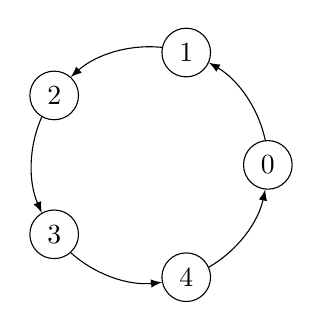
\begin{tikzpicture}[scale=0.5]
\def \n {5}
\def \radius {3cm}
\def \margin {12} 

\foreach \s[count=\xi from 0] in {1,...,\n}
{
  \node[draw, circle] at ({360/\n * (\s - 1)}:\radius) {$\xi$};
  \draw[->, >=latex] ({360/\n * (\s - 1)+\margin}:\radius) 
    arc ({360/\n * (\s - 1)+\margin}:{360/\n * (\s)-\margin}:\radius);
}
\end{tikzpicture}
\end{codeexample}








% \chapter{Endnotes}

There a number of packages that can help you add endnotes to your document.
This can be added at the end of every document or at the end of every chapter.

The first package we will use is \ctan{pagenote}. This was developed by Peter Wilson, 
and now maintained by Will Robertson. The pagenote package provides notes similar to footnotes except that
they are typeset on a different page. These are often called end notes.
Unless the memoir class is being used, the package requires the \ctan{ifmtarg}
package to be installed as well.

The package manager provides a key,


\begin{docKey}[phd]{endnotes pagenote=\meta{pagenote or endnotes (default pagenote)}  }{}{}
 Set the key using |\cxset{endnotes package=pagenote}|.
\end{docKey}

One need to be careful, of the other commands required, in the preamble when you load the package. For example the |pagenote| package, requires that a |\makepagenote| command is issued in the preamble.
The entries are written in an auxiliary file with the extension |.ent|. 

\emphasis{document,usepackage,pagenote,printnotes,
          makepagenote,usepackage}

\begin{teXXX}
\documentclass{book}
\usepackage{pagenote}
\makepagenote
\renewcommand*{\notedivision}{\section*{%
   \notesname\ to chapter~\thechapter}}
\renewcommand*{\pagenotesubhead}[2]{}
\begin{document}
\chapter{bar}
  \section{blubb}
   Some text.\pagenote{The first endnote.}
\printnotes*

\chapter{foo}
  \section{foobar}
   Some text.\pagenote{The second endnote.}
   Some text.\pagenote{}
\printnotes*
\end{document}
\end{teXXX}

The \cmd{\printnotes} command will cause the |.ent| file to be closed for any new
\cmd{printnotes*} notes, and then |\input| in order to print the collected notes. After |\printnotes|
no more notes will be collected, so use it after all are done.

The \ctan{endnotes} package works in a similar manner. To place all endnotes at the end of the chapter Each time you use \cmd{\theendnotes}, all endnotes that were stored previously will be put there. So just write \cmd{\theendnotes} at the end of each chapter.



Footnotes are notes\pagenote{There is a long discussion about the pros and cons of end notes in the Wikipedia.} at the foot of the page while endnotes are collected under a separate heading at the end of a chapter in a book or a document. Unlike footnotes, endnotes have the advantage of not affecting the image of the main text, but may cause inconvenience to readers who have to move back and forth between the main text and the endnotes\pagenote{The polynomial \[ polynomial{1,2,3,4,5} \] is a case in point. You can typeset a polynomial by using the \texttt{polynomial} package or if you are using special polynomials you should have a look at the \texttt{cool} package}.

The U.S. Government Printing Office Style Manual devotes over two pages to the topic of footnotes.[2] NASA has guidance for footnote usage in its historical documents.[3] About rules \pagenote{\notei}

\url{http://tex.stackexchange.com/questions/210/how-can-i-get-two-sequences-of-footnotes-in-one-latex-document-one-as-footnote}

 "The user may want separate endnotes for each chapter, or a big block of them at the end of the whole document. As it stands, either will work; you just say \cmd{theendnotes} wherever you want the endnotes so far to be inserted. However, you must add |\setcounter{endnote}{0}| after that if you want subsequent endnotes to start numbering at 1 again." 

\section*{Footnote and end note font sizes}

This is normally specified by the publications Style Manual. It is normal to use smaller type approximately 3-4 points smaller than the main text\pagenote{\noteii}\pagenote{\noteiv}.


\section*{Footnote marks}

Again for the footnote marks the publication Style manual should be consulted\pagenote{\noteiii}.

When symbols or signs are used for footnote reference marks, their 
sequence should be (*) asterisk, (\dag) dagger, (\ddag) double dagger, and 
(\S) section mark. Should more symbols be needed, these may be 
doubled or tripled, but for simplicity and greater readability, it is 
preferable to extend the assortment by adding other single-character symbols.(US Government Style Manual). \latex provides eleven marks and these should adequately cover most cases. End notes are normally marked in sequential superior numbers.
\footnote{See also Chapter 8}

\section*{Separation of footnotes}

When two or more footnotes occur together use a thin space to separate them.
\pagenote{From the U.S. Governement Style Manual p.305, \S 15.19. Two or more superior footnote references occurring together are separated by thin spaces.}
\tex and most of the packages will adequately allow for this.


\section{Some tips}

If your footnotes and endnotes tend to be rather long, they can interefere with the editing of the works. In such case you can define some macros and accumulate these some where either at the beginning or end of the Chapter. Remember you cannot use numbers as variable names. An example of such a macro is shown below:

One question that comes quite often is:

I find it common in my writing to end up a sentence with a footnote reference mark. Should the footnote mark come before the stop or after it?

... this is some text$^a$.

... this is some text.$^b$


but in the world of typesetting, logic is not respected. At least in the field of scientific publishing, where footnotes and references are common, publishers tend to have very strict guidelines about where they want the marks. In that case, you're not really free to choose yourself. For example, most of the physics and chemistry journals want references after punctuation:

Both are valid ways to place a footnote reference, but they mean slightly different things.

If you want the footnote reference to belong to the entire sentence, then the second method is correct. However, if you want the footnote to apply only to the word text, then the first is correct.\footnote{AAAAAA}

See also \pagenote{For a discussion see \href{http://english.stackexchange.com/questions/9632/footnote-marks-at-end-of-a-sentence}{footnotemarks}}

\emphasis{def,notei}
\begin{teXXX}

\def\notei{\footnotesize{p[116] of \textit{The Printer's Grammar}, printed by L. Waylard,1775. writes about metal rules. Metal rules, like quadrats, are cast to m's, in such founts as are commonly employed in figure-work; which are casr to most of the small bodies. Metal rules are used in Schemes of Accounts, to direct and conect each Article with its summary contents, where they stand oposite, and distant from each other: in which case all the different sizes of rules are used, to prevent one rule falling upon another, especially of the same force;}}
\end{teXXX}

\def\notei{\footnotesize{p[116] of \textit{The Printer's Grammar}, printed by L. Waylard,1775. writes about metal rules. Metal rules, like quadrats, are cast to m's, in such founts as are commonly employed in figure-work; which are casr to most of the small bodies. Metal rules are used in Schemes of Accounts, to direct and conect each Article with its summary contents, where they stand oposite, and distant from each other: in which case all the different sizes of rules are used, to prevent one rule falling upon another, especially of the same force;}}




\def\noteii{\footnotesize{U.S. Government Style Manual (2008), 30th Edition, recommends that unless the copy is otherwise marked: (1) Footnotes to 12-point text 
are set in 8 point; (2) footnotes to 11-point text are set in 8 point, 
except in Supreme Court reports, in which they are set in 9 point; 
(3) footnotes to 10- and 8-point text are set in 7 point.}}

\def\noteiii{\footnotesize{For reference marks use: (1) Roman superior figures, (2) italic superior letters, and (3) symbols. Superior figures (preferred), letters, and symbols are separated from the words to which they apply by thin 
spaces, unless immediately preceded by periods or commas.}}

\def\noteiv{\footnotesize{Manual of Typography, pg 44 Foot-notes are set smaller than the text. There is no absolute rule, but generally it is two or three sizes less. If the text were in pica the notes might be set in brevier, or
even nonpareil. The same holds good for small pica or
long primer. Foot-notes have references in the text, and
when being set should be "flagged": that is, a piece of
paper inserted in the type stating what it is, to guide the
maker up, so that he can place it in its proper position.}}


\footnoterule

\renewcommand*{\notedivision}{\section*{\notesname\ to chapter~\thechapter}}
\renewcommand*{\pagenotesubhead}[2]{}

\printnotes



\normalsize








% 
% \input{./sections/elgreco}
% 
% \input{./sections/book.cls.tex}
% %\newcommand\addcredit[1]{%
 \bgroup
 \vspace*{-6.5pt}
 \scriptsize%
  \tcbox[colframe=white,
        colback=white,
        size=minimal, 
        nobeforeafter,
        minipage,
        boxsep=0pt,
        top=0pt, 
        bottom=0pt,
        shrink tight,
        right=0pt,left=0pt]{\hfill\hfill\textit{Credit: #1}}%
 \egroup
}


\chapter{Drawing pictures and graphs}

\epigraph{Dear God\break If I have but one hour remaining to live, please allow me to spend this time
in a mathematics class so that it will seem to last forever.}{\textit{---A bored student's prayer}}





\section{Inserting figures}

In order to insert figures, the \pkgname{graphicx} package has to included in the preamble (before the |\begin{document}|-command) of your LaTeX-document:

\begin{dispListing}
\usepackage{graphicx}
\end{dispListing}

Originally only EPS-figures could be inserted with the \pkgname{graphic}package. This has now been developed into the  \pkgname{graphicx}, which allows almost any common format to be inserted. 

The simplest way of including a graphic looks like this:


\begin{docCommand}{includegraphics}{ \marg{filename}}{}
Includes the graphic into the document.
\end{docCommand}

\begin{figure}[htbp]%
  \centering
  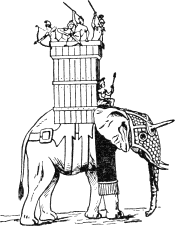
\includegraphics[width=0.3\linewidth]{./graphics/pic37.png}
  \caption{During the early days of typography fonts were designed to emulate the looks of calligraphic texts.}
  \label{fig:marginfig1}
\end{figure}

If the image is not located in the same folder as the tex-file, you will have to specify the path relative to the tex-file. This is a source of problems for many 

\begin{verbatim}
\includegraphics{./images/filename}
\end{verbatim}


\subsection{Scaling and resizing images}

If you want the image to appear in a different size, you can specifiy the size as a parameter of the |\includegraphics|-command::

\begin{commands}[]{ex:graphics}
\cmd{\includegraphics}\oarg{width=3.9cm}\marg{filename}
\end{commands}

This will scale the image to the width of 3.9 centimeters. 

Use |\textwidth| command if you don't want to specify an absolute size but rather want the actual size to depend on the text width of the page. You can use any of the normal \tex units such as \texttt{em, pt, cm, in}:

\begin{commands}[]{ex:graphics}
\cmd{\includegraphics}\oarg{width=0.5\string\textwidth}\marg{filename}
\end{commands}

\noindent will scale the image to half of the text width. The images in the
figure below were produced by three |\includegraphics| commands. You can have as many as you like and the \tex engine will treat them the same way as text. If you a leave a space between the commands, they will be positioned vertically as they are treated as paragraphs.

\medskip

\begin{commands}[]{}
\begingroup

\centering
\includegraphics[width=0.3\textwidth]{./graphics/amato.jpg}
\includegraphics[width=0.3\textwidth]{./graphics/amato.jpg}
\includegraphics[width=0.3\textwidth]{./graphics/amato.jpg}

\endgroup

\begin{verbatim}
\begingroup

\centering
\includegraphics[width=0.3\textwidth]{./graphics/amato.jpg}
\includegraphics[width=0.3\textwidth]{./graphics/amato.jpg}
\includegraphics[width=0.3\textwidth]{./graphics/amato.jpg}

\endgroup
\end{verbatim}
\captionof{figure}{Images aligned horizontally.}
\end{commands}

The three photos were centered using the |\centering| command, within a group. The |\begingroup..\endgroup| is necessary to limit the effect of centering to
the group only, otherwise \tex would center everything from this point onwards.

\subsection{Controlling the aspect ratio}

You can control the picture aspect ratio by using the command:

\begin{docCommand}{includegraphics}{\oarg{keepaspectratio,width=3cm, height=3cm}\marg{filename}}
\end{docCommand}

If the key |keepaspectratio| is set to true then specifying 
both |width| and |height| (or |totalheight|) does not distort the figure but 
scales such that neither of the specified dimensions is exceeded.


\endinput

\medskip
\begin{commands}[]{}
\begingroup

\centering
\includegraphics[width=0.3\textwidth, height=5cm]{./images/amato.jpg}
\includegraphics[keepaspectratio=true,width=4cm, height=5cm]{./images/amato.jpg}
\includegraphics[width=3cm]{./images/amato.jpg}

\endgroup

\begin{verbatim}
\begingroup

\centering
\includegraphics[width=0.3\textwidth, height=5cm]{amato}
\includegraphics[keepaspectratio=true,width=4cm, height=5cm]{amato}
\includegraphics[width=3cm]{amato}

\endgroup

\end{verbatim}
\captionof{figure}{Controlling the aspect ratio.}
\end{commands}

This can be very useful if you have images shown side by side with different
aspect ratios. 


\subsection{Paths and file types}

For larger projects you will probably find it more convenient to have 
images in different folders. You can specify default paths using:


\begin{docCommand}{graphicspath} {\marg{dir-list}} {}
\end{docCommand}

This optional declaration may be used to specify a list of directories in which to
search for graphics files. The format is the same as for the \latexe primitive
|\input@path|. A list of directories, each in a \{\} group (even if there is only one
in the list). For example:

\begin{dispListing}
\graphicspath{{eps}{tiff}}}
\end{disListing}

The default image formats can be declared using:

\begin{docCommand}{DeclareGraphicsExtensions}{ \marg{png, jpg, eps, jpeg}}{}
\end{docCommand}

This specifies the behaviour of the system when no file extension is specified in 
the argument to |\includegraphics|. \texttt{\{ext-list\}} should be a comma separated 
list of file extensions. (White space is ignored between the entries.) A file name
is produced by appending one extension from the list. If a file is found, the
system acts as if that extension had been specified. If not, the next extension
in \texttt{ext-list} is tried.



\subsection{The figure environment}

You use the figure-environment to let your image appear in a \emph{floating} environment, that is \latex will place it at the right position of a page and even on the next page:

\begin{teX}
\begin{figure}
  \includegraphics{filename.jpg}
  \caption{title of your figure}
  \label{labelname}
\end{figure}
\end{teX}

Here |\caption{...}| defines the title of the figure which will appear beneath the figure. |\label{..}| defines the label which can be used inside the document in order to insert references to the figure:

The figure

|\ref{labelname} on page \pageref{labelname} ..|

The|\label-command| inside the |\figure|-envirnonment hast to appear just after the|\caption|-command.
placing figures

If figures reside inside a |\figure|-environment, this will cause LaTeX to choose the actual location of the figure inside the document. There are different parameters for the placement strategy:

\begin{description}
\item[h (here)] Try to place the figure just where the command is located.

\item [t (top)] Try to place the figure at the top of the page.

\item[b (bottom)] Try to place the figure at the bottom of the page.

\item [p (float page)] Try to place the figure on a page which contains only floating elements.
\end{description}

The order of these parameters doesn't matter since placement is always tried in the order \textbf{h, t, b, p,} if these parameters are present:

If no parameter is present, the default order is  \texttt{[tbp]}.


The command for a figure-environment might for example look like this:

\begin{teX}
\begin{figure}[htbp]
...
\end{figure}
\end{teX}



\subsection{List of figures}
\index{figures!Table of figures}
A table of figures is inserted (where you place the command) using the command


\begin{teX}
   \listoffigures
\end{teX}

The caption given in the \cmd{caption} command is also used in the list of figures. 
If you want to use different captions, you may add a parameter to the |\caption| command:
|\caption[caption for listoffigures]{caption inside the document}|


\subsection{Figures with a border}

Although drawing frames around tables should be discouraged, if you find the need
to draw them there are  two possible ways to achieve it: either only the figure itself is bordered or there is a border around the figure and its caption. You place a border around the figure using the \cmd{\fbox} command or the \cmd{\framebox}.

\emphasis{fbox,minipage}
\begin{teX}
\begin{figure}[htbp]
  \centering
  \fbox{%
    \includegraphics{filename}%
  }%
  \caption{caption}
  \label{Labelname}
\end{figure}
\end{teX}

Placing a border around the figure and its title is a little more tricky: You need to place the figure and the title in a |\minipage| environment which is bordered again with the |\fbox| command:

\begin{figure}[htbp]
\centering
  \fbox{
    \begin{minipage}{.95\linewidth}
      \mbox{}%
      \centering
      
      \includegraphics[width=.9\linewidth]{./images/asia.jpg}%
      \caption{How to place a border around an image. }%
      \label{labelname}%
    \end{minipage}}
 
\begin{verbatim}
\begin{figure}[htbp]
  \centering
    \begin{minipage}{width=.8\linewidth}
     \centering
     
      \includegraphics[.9\linewidth]{filename}
      \caption{caption}
      \label{labelname}
    \end{minipage}
 \end{figure}
\end{verbatim}

\end{figure}



Unfortunately the width of the border cannot be determined automatically. It has to be specified as a parameter of the |\minipage| environment. However, you may be bale to develop a macro to do this,  based on the ImageSize routines we developed in section.


\section{Complex Layouts}
\label{looting}
In reality most professionally typeset books will have their own style for image pages. In Figure~\ref{complex}
three images are set in a non-symmetrical layout. This type of setting is difficult to automate and manual intervention is possible.

This layout will require four minipages. Two for the top figure (one for the image and one for the caption) and two for the two bottom figures. The rightmost bottom figure will have to be put in a zero height box to let it overflow to the top. The figure has been reproduced from an Oriental Institute publication \emph{Catastrophe! The Looting and Destruction of Iraq’s Past} \cite{looting}. The book is interesting both for its contents as well as its simple but effective typography and appropriate for the topic. The volume has been pblished in conjuction with the exhibition titled as the name of the book, that described the loss of Iraq’s archaeological past to looters and to the war. 

\begin{figure}[p]
\centering
\includegraphics[height=0.8\textheight]{oriental}
\addcredit{Oriental Institute}
\caption{More complex layouts. \emph{Copyright the Oriental Institute of the University of Chicago.}}
\label{complex}
\end{figure}

The style is reproduced in a \pkgname{phd} template (style 56) and both code and details can be found in the relevant pages.





\section{Side by side figures}

You might want to place to figures side by side but to use only one caption. This is achieved by placing both figures in its own |\minipage| which reside in the same |\figure|.

if only one |\caption| command is used, both figures will have a common title:

\medskip
\begin{verbatim}
\begin{figure}[htbp]
  \centering
  \begin{minipage}[b]{5 cm}
    \includegraphics{filename 1}  
  \end{minipage}
  \begin{minipage}[b]{5 cm}
    \includegraphics{filename 2}  
  \end{minipage}
  \caption{common caption}
  \label{Labelname}
\end{figure}
\end{verbatim}
\medskip

The first parameter of the |\minipage| environment determines how both graphics are aligned to each other. b (bottom) aligns the bottom borders of the figures, \textbf{t} (top) aligns the top borders and \textbf{c} aligns the centers.

If you want distinct titles for the two figures you will only have to supply a |\caption| command for both |\minipage|environments:

\begin{teX}
\begin{figure}[htbp]
  \centering
  \begin{minipage}[b]{5 cm}
    \includegraphics{filename 1} 
    \caption{caption 1}
    \label{labelname 1}
  \end{minipage}
  \begin{minipage}[b]{5 cm}
    \includegraphics{filename 2}  
    \caption{caption 2}
    \label{labelname 2}
  \end{minipage}
\end{figure}
\end{teX}


If you want to have subfigures with distinct caption, you use the |\subfig| package:


You can put as many figures as you like on a page, but a word of warning, you may need to make some manual adjustments before you get it right. The package provides support for the manipulation and reference of small or ‘sub’ floats within a single floating (e.g., figure or table) environment1 It is convenient to use this
package when your sub-floats are to be separately captioned, referenced, or when such
sub-captions are to be included on a List-of-Floats page.

The package is a replacement for the subfigure package, from which it was derived.
However, the new subfig package is not completely backward compatible.
Therefore, a new name was called for. The newer package is smaller and easier to use
than the older package, however, it now uses the following additional packages, 
caption (required), 
everysel (optional), 
keyval (required), 
ragged2e (optional).

It will work without the \pkgname{ragged2e} and \pkgname{everysel} packages if you do not use the following
justification options: ‘Center’, ‘RaggedRight’ and ‘RaggedLeft’. The other justification
options ‘center’, ‘raggedright’ and ‘raggedleft’ will work without the above two packages. If the ragged2e package is present, than the caption package will load it and it
will, in turn, load the everysel package. This happens whether or not you will be using
the justification options that require it. If it cannot find the ragged2e package, than the
caption package will print a message that ‘RaggedRight’, etc. will not be available.


\begin{figure}[htb]
\includegraphics[height=5cm]{dotty}
\includegraphics[height=5cm]{bette}
\includegraphics[height=5cm]{dotty}
\end{figure}

 A low bottle-shaped vase, of yellowish ware, with flaring rim and somewhat flattened body. Height, 5 inches; width 5 inches. \ref{fig:one}

A well-made bottle shaped vase, with low neck and globular body, somewhat conical above. Color dark brownish. 7½ inches in height. Shown in \ref{fig:two}


\begin{figure}
  \centering
  \includegraphics[width=0.7\linewidth]{./graphics/fig175.jpg}
   \centerline{From the tomb of a Pull\= arius.}
  \label{fig:marginfig1}
\end{figure}

The above figure is an effigy vase of the dark ware. The body is globular. A kneeling human figure forms the neck. The mouth of the vessel occurs at the back of the head—a rule in this class of vessels. Is is finely made and symmetrical. 9¾ inches high and 7 inches in diameter. being larger than the above two it is preferable to scale it to give the reader an indication. Based on the figure width, you may also need to adjust the distance between the figures to ensure that the whitespace is just about right. For screen reading this can be increased and for printed works you may wish to make it less.



\section{The wrapfig package}


\captionsetup[wrapfigure]{margin=10pt,font=small,labelfont=bf, name=Fig.} % [wrapfigure]{name=Fig.}


Donald Arseneau has created the \pkg{wrapfig} package\footfullcite{wrapfig} to allow people to place figures or
tables at the side of a page and wrap text around them. The package provides the
environments \docAuxEnv{wrapfigure} and \docAuxEnv{wraptable}. Both environments have two required and
two optional arguments. You can see an example that uses the package to wrap a picture into such a paragraph of text.

\begin{figure}[htbp]
   \includegraphics[width=\linewidth]{./graphics/cyprus.jpg} 
   \caption{Cyprian limestone group of Phoenician dancers, about 6½ in. high. There is a somewhat similar group, also from Cyprus, in the British Museum. The dress, a hooded cowl, appears to be of great antiquity.}
\end{figure}

\begin{wrapfigure}[20]{l}{3.8cm}
\centering\small
\includegraphics[width=\linewidth]{./graphics/egyptdance.jpg}  
\caption{The hieroglyphics describe the dance.}
\end{wrapfigure}
Amongst the earliest representations that are comprehensible, we have certain Egyptian paintings, and some of these exhibit postures that evidently had even then a settled meaning, and were a phrase in the sentences of the art. Not only were they settled at such an early period (B.C. 3000, fig. 1) but they appear to have been accepted and handed down to succeeding generations (fig. 2), and what is remarkable in some countries, even to our own times. The accompanying illustrations from Egypt and Greece exhibit what was evidently a traditional attitude. The hand-in-hand dance is another of these.

The earliest accompaniments to dancing appear to have been the clapping of hands, the pipes,[1] the guitar, the tambourine, the castanets, the cymbals, the tambour, and sometimes in the street, the drum.

The following account of Egyptian dancing is from Sir Gardiner Wilkinson's "Ancient Egypt"[2]:—
\begin{figure}
   \includegraphics[width=0.3\linewidth]{./graphics/lotus.jpg} 
   \caption{Cyprian limestone group of Phoenician dancers, about 6½ in. high. There is a somewhat similar group, also from Cyprus, in the British Museum. The dress, a hooded cowl, appears to be of great antiquity.}
\end{figure}
"The dance consisted mostly of a succession of figures, in which the performers endeavoured to exhibit a great variety of gesture. Men and women danced at the same time, or in separate parties, but the latter were generally preferred for their superior grace and elegance. Some danced to slow airs, adapted to the style of their movement; the attitudes they assumed frequently partook of a grace not unworthy of the Greeks; and some credit is due to the skill of the artist who represented the subject, which excites additional interest from its being in one of the oldest tombs of Thebes (B.C. 1450, Amenophis II.). Others preferred a lively step, regulated by an appropriate tune; and men sometimes danced with great spirit, bounding from the ground, more in the manner of Europeans than of Eastern people. On these occasions the music was not always composed of many instruments, and here we find only the cylindrical maces and a woman snapping her fingers in the time, in lieu of cymbals or castanets.

\begin{figure}
   \includegraphics[width=0.3\linewidth]{./graphics/patera.jpg} 
   \caption{Cyprian limestone group of Phoenician dancers, about 6½ in. high. There is a somewhat similar group, also from Cyprus, in the British Museum. The dress, a hooded cowl, appears to be of great antiquity.}
\end{figure}

"Graceful attitudes and gesticulations were the general style of their dance, but, as in all other countries, the taste of the performance varied according to the rank of the person by whom they were employed, or their own skill, and the dance at the house of a priest differed from that among the uncouth peasantry, etc.

"It was not customary for the upper orders of Egyptians to indulge in this amusement, either in public or private assemblies, and none appear to have practised it but the lower ranks of society, and those who gained their livelihood by attending festive meetings.

"Many of these postures resembled those of the modern ballet, and the pirouette delighted an Egyptian party 3,500 years ago.
\medskip

The wrapped figure is positioned using the \texttt{wrapfigure} environment, as shown below:

\begin{teX}
\begin{wrapfigure}[nlines]{placement}[overhang ]{width }
   \includegraphics[width=3.8cm]{./graphics/egyptdance} 
   \caption{The hieroglyphics describe the dance.}
\end{wrapfigure}
\end{teX}

The parameter |nlines|  is the number of narrow lines, and placement is one of r, l, i, o, R, L, I, or
O for right, le, inside, and outside, respectively. The uppercase placement specifiers
differ from their lowercase counterparts in that they force \latex to put the float \emph{here},
whereas the lowercase placement specifiers just give a hint to \latex to place them
\texttt{here}. The \meta{width} argument is the width of the figure or table that appears in the body
of the environment. Finally, \texttt{overhang} tells \latex how much the figure should hang out
into the margin of the page. Here is how one may create dangerous paragraphs bends!

The |wrapfig| package is compatible with the |caption| package. You can set the caption parameters using:---

\begin{teX}
\captionsetup[wrapfigure]{<options>}
\end{teX}

If you are probably wondering how |wrapfig| achieves this, you should read the package code. It basically uses \refCom{everypar}, and hence the limitations with |\par|. Here is an extract from the class.

\begin{teX}

% Subvert \everypar to float fig and do wrapping.  
% Also for non-float.
\def\WF@startfloating{%
 \WF@everypar\expandafter{\the\everypar}\let\everypar\WF@everypar
 \WF@@everypar{\ifvoid\WF@box\else\WF@floathand\fi \the\everypar
 \WF@wraphand
}}
\end{teX}

Moving now to a more scientific example that the previous ones, we will place two figures
one on top of each other and give them individual, sub-captions as shown in \ref{fig:honey}.
 
\captionsetup[figure]{margin=10pt,font=small,labelfont=bf,format=hang}%

\begin{figure}[htbp]
\centering
  \begin{subfigure}[b]{0.5\textwidth}
  \includegraphics[width=\linewidth]{./graphics/honey.png}
  \caption{Taylor instability in the surface of the honey in an inverted honey jar.}\label{fig:honey}
    \hspace{1cm}
  \end{subfigure}

  \begin{subfigure}[b]{0.9\textwidth}
     \centering
     \includegraphics[width=9cm]{./graphics/honeydrops.png}
     \caption{Taylor instability in the interface of the water condensing on the underside of a small water pipe.}
  \end{subfigure}  
  \caption{Two examples of Taylor instabilities that are commonly found.}%
    \label{fig:Athird}%
\end{figure}

The figures are from \textit{A Heat Transfer Textbook}, by J.H.Lienhard, which incidentally was typeset using
\tex . It is a McGrawHill publication. 

\begin{teX}
\begin{figure}[htbp]
    \captionsetup[figure]{margin=10pt}%
    \subfloat[Taylor instability...]
     {{\includegraphics[width=8cm]{./graphics/honey}}}
    \hspace{1cm}
     \subfloat[Taylor instability in the...]%
      {\includegraphics[width=9cm]{./graphics/honeydrops}}  
     \\[-10pt]
   \caption{Taylor instability in...}%
    \label{fig:Afirst}%
    \caption{Two examples of... }%
    \label{fig:honey}%
\end{figure}
\end{teX}


The text can have more than one paragraph. It is also possible to include figures
generated by |TikZ/pgf|, as shown in the next example, drawn from real code
in the book.


%\begin{wrapfigure}[14]{l}{3.0cm}
%\pgfplotsset{width=5.0cm,compat=1.3}
%\begin{tikzpicture}
%\begin{axis}[minor y tick num=4, 
%minor x tick num=4, 
%xmin=0,xmax=300,
%ymin=0,ymax=60,
%xlabel=\textsf{liquidus ($l/s$)},
%ylabel=\textsf{capitis ($m$)}, 
%ytick={0,15,30,45,60,75},
%xtick={0,100,200,300}
%]
%\addplot[color=blue,mark=x, smooth] coordinates {
%(0,44)
%(50,43)
%(100,42)
%(150,40)
%(200,33)
%(220,29)
%};
%
%\end{axis}
%\end{tikzpicture}
%\captionof{figure}{Pump headum and flowm}
%%\end{wrapfigure}



\begin{figure}[htp]
\centering

\captionsetup{name=Photo., labelsep=period, format=plain}%
   \begin{minipage}[t]{0.48\textwidth}
      \includegraphics[width=\textwidth]{./graphics/movingup.jpg}%
      \vskip1pt\addcredit{U.S. DoD.}%
     \caption{The effects of the credit going past the edge of the figure. This can be corrected by adding a minipage to hold both commands. }
\end{minipage}\hfill\hfill
\begin{minipage}[t]{0.48\textwidth}
      \includegraphics[width=\textwidth]{./graphics/survivors.jpg}%
      \addcredit{U.S. DoD.%
    {\footnotesize Marines awaiting resting before moving on to Japan. }}%
    \flushleft
    \caption[Adding a credit to an image.]{The effects of the credit going past the edge of the figure. This can be corrected by adding a minipage to hold both commands. }
    
\end{minipage}
% \begin{minipage}[t]{0.48\textwidth}
%      \includegraphics[width=\textwidth]{./graphics/img009.jpg}%
%      \addcredit{U.S. DoD.}%
%     \caption{Engineer Construction Troops in Liberia, July 1942.}
%\end{minipage}\hfill\hfill
%\begin{minipage}[t]{0.48\textwidth}
%      \includegraphics[width=\textwidth]{./graphics/survivors.jpg}%
%      \addcredit{U.S. DoD.}%
%     \caption{The effects of the credit going past the edge of the figure. This can be corrected by adding a minipage to hold both commands. }
%\end{minipage}
% \begin{minipage}[t]{0.48\textwidth}
%      \includegraphics[width=\textwidth]{./graphics/img126.jpg}%
%      \addcredit{U.S. DoD.}%
%     \caption{Marine Reinforcements.
%A light machine gun squad of 3d Battalion, 1st Marines, arrives during the battle for ``Boulder City.'' }
%\end{minipage}\hfill\hfill
%\begin{minipage}[t]{0.48\textwidth}
%      \includegraphics[width=\textwidth]{./graphics/img124.jpg}%
%      \addcredit{U.S. DoD.}%
%     \caption{Brothers Under the Skin, inductees at Fort Sam Houston, Texas, 1953. }
%\end{minipage}
\par
\end{figure}


Armed with all these packages you can help the Gutenburg organization to transcribe
some of the old books that they have online. 









 
% %\let\luacmd\textbf
\chapter[Charts and Visualizations]{Presenting Data in Charts and Visualizations}
\label{ch:charts}
\pagestyle{headings}

There can be no doubt that the hallmark of scientific reports and publications is the graphical presentation of the results. Graphs show relationships underlying observations in a way no other device can provide\footnote{\textit{Doing science: design, analysis, and communication of scientific research}
 By Ivan Valiela}.  Charting is both an art and a science. Modern typography on charts and infographics look at Tufte as inspiration.
Tufte advocates to minimize the ink to data ratio and although this is not always possible it is good advice.
In this section we would look at charting in general which is probably of interest to most of the readers
in this book.  Another good source of information is Stephen Few’s website the \href{perpetualedge}{perceptualedge} \footnote{\protect\url{http:\\perceptualedge.com}}  with a number of excellent articles on data visualization. 



\captionsetup[figure]{name=Photo,parindent=0pt,minmargin=0pt,width=3sp,labelsep=period,skip=5pt,margin={0pt,0pt},margin*={0pt,0pt},position=bottom,singlelinecheck=on}

\begin{figure}[htbp]
\parindent=0pt
\centering

\includegraphics[width=0.8\linewidth]{./images/medieval-calendar.png}

\parindent-1em
\noindent\caption{This 1496 manuscript shows medieval calendars with depictions of the positions of the Sun and the Moon.}

\end{figure}

This chapter will focus more on charting rather than visualizations, as widely understood. These are best painted with a different tool. 

\begin{figure}[htbp]
\parindent=0pt


\includegraphics[width=\textwidth]{beautiful-evidence}

\caption{An extract from Tufte’s book \textit{Beautiful Evidence}. In his book Tufte advocates that science and art have in common \emph{intense seeing}, the wide-eyed observing that generates empirical information. \textit{Beautiful Evidence} is about how \emph{seeing} is turned into \emph{showing}. \cite{Tufte2006}}
\end{figure}

\section{Graphical Perception}

When a person looks at a graph, the information is decoded by the person’s visual system. A graphical method is successful only if the decoding is effective. Cleveland \cite{cleveland1985} in an often quoted study designed experiments and made suggestions as to how graphical data can be improved by selecting representations that have high rank in Table~ref{tbl:cleveland}. Cleveland and McGill at the time employed as statistical scientists at At \& T Bell Laboratories, investigated how we perceive quantitative information and produced a table as to how to order elementary tasks by accuracy. They suggested graphs should exploit tasks as high in the ordering as possible. The tasks are ordered from most accurate to least.


\begin{longtable}[c]{l>{\RaggedRight}p{7.5cm}}
\caption{Rank table for chart visual representation.}\label{tbl:ranktable} \\
\toprule
Rank  & Position along a common scale\\
\midrule
1  & Position along a common scale\\
2  & Position on identical but nonaligned scales\\
3  & Length\\
4  & Angle\\
    & Slope (with $\theta$ not too close to 0, $\pi/2$, or $\pi$ radians)\\
5   & Area\\
6   &Volume\\
     &Density\\
     &Colour saturation\\
7   & Colour hue\\         
\bottomrule
\end{longtable}





\begin{figure}[htbp]
\includegraphics[width=0.45\textwidth]{length-judgement}
\caption{The top panel is a divided bar chart. This graphical method requires length judgement; for example
to compare and order the values in group A is not easy. In the bottom panel the values are shown by a dot
chart. All values on the graph can be visually compared by judgements of position along a common scale, an
easier task. Now the ordering of the values in group A is easy to perceive. Adapted from \cite{cleveland1985}.}
\end{figure}

\section{How to Draw your Charts}

With the newer engines the limitations of fonts are now part of TeX’s history, so you can use other programs. However, the use of PGF and TikZ or pstricks is still an unbeatable way to produce high quality charts and graphs.
For visualizations other tools might be necessary. Asymptote is on of them and I am sure you have other in your toolbox.

\section{Tufte like charts}

During the last stages of a Project, it maybe easier to visualize the
main areas where effort needs to be exerted by using simple charts. One
such chart is shown in Figure~\ref{fig:tufte-overall}. When this chart
was prepared efforts were made to complete the physical installation
as well as plan and commission the plant. The use of colour in this
chart highlights the commissioning, so one can easily see the expectations. Although the percentages are written on top of the bars,
one need not read them to visualize how difficult is to achieve
100\% completion in a Project. On the other hand commissiong can go
fairly fast and can jump by a large percentage, just by
commissioning a couple of additional ELV systems that have approximately
a 10\% weigh factor.

One can easily fit approximately, six to seven months data on
a portrait chart, changing it around to landscape one can fit
more than a year. Personally I am not very happy with such long
projections as they are more like guesses rather than proper estimates.

One other chart that can be used to visualize progress and is more
commonly found in construction is the infamous S-curve. Now, if
the actual planning is detailed enough and granular enough to be
able to pin-point \textit{continuous} progress then it is
appropriate. using it if you can at least obtain weekly progress
estimates.


 
\begin{figure}[htbp]
\parindent0pt
\hspace*{-1.8cm}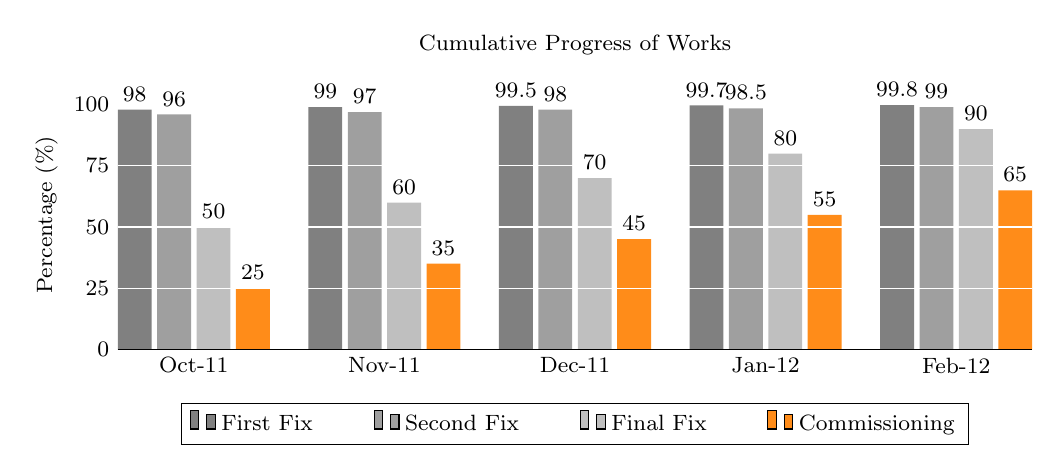
\begin{tikzpicture}
\footnotesize%

  \begin{axis}[
        ybar, axis on top,
        title={Cumulative Progress of Works},
        height=5cm, width=13.2cm,
        bar width=0.43cm,
        ymajorgrids, tick align=inside,
        major grid style={draw=white},
        enlarge y limits={value=.1,upper},
        ymin=0, ymax=100,
        axis x line*=bottom,
        axis y line*=left,
        y axis line style={opacity=0},
        ytick={0,25,50,75,100},
        tickwidth=0pt,
        legend style={
            at={(0.5,-0.2)},
            anchor=north,
            legend columns=-1,
            % adds space between the legends
            /tikz/every even column/.append style={column sep=0.7cm}
        },
        ylabel={Percentage (\%)},
        symbolic x coords={
           Sep-11,Oct-11,Nov-11,Dec-11,
           Jan-12,Feb-12,
           Mar-12,
           Apr-12},
       xtick=data,
       nodes near coords={
        \pgfmathprintnumber[precision=2]{\pgfplotspointmeta}
       }
    ]
    \addplot [draw=none, fill=gray] coordinates {
      (Oct-11, 98)
      (Nov-11,99)
      (Dec-11,99.5)
      (Jan-12,99.7)
      (Feb-12,99.8)
       };
   \addplot [draw=none,fill=gray!75!white] coordinates {
      (Oct-11, 96)
      (Nov-11,97)
      (Dec-11,98)
      (Jan-12,98.5)
      (Feb-12,99)
        };
   \addplot [draw=none, fill=gray!50!white] coordinates {
      (Oct-11, 50)
      (Nov-11, 60)
      (Dec-11, 70)
      (Jan-12, 80)
      (Feb-12, 90)
            };
    \addplot [draw=none, fill=orange!90!white] coordinates {
      (Oct-11, 25)
      (Nov-11, 35)
      (Dec-11, 45)
      (Jan-12, 55)
      (Feb-12, 65)
          };
    \legend{First Fix,Second Fix,Final Fix,Commissioning}
  \end{axis}
  \end{tikzpicture}\par
  
\captionsetup[figure]{name=Photo, labelsep=period,
                    skip=5pt, font=scriptsize,
                    position=bottom, margin{0pt,0pt}}
                    
\caption{Cumulative progress for all MEP works. Notice the slower rate of production during the last three months.}

\label{fig:tufte-overall}

\end{figure}


A good graph is uncluttered, clear and focused.

\subsection{Axis Lines}

Most problems with graphs arise from misuse of axes: too heavy, too long, wrong intersection,
ambiquous breaks or too confusing increments and incorrect proportions. An axis is a ruler that established
regular intervals for measuring the information provided. Axes may emphasize, diminish, distort, simplify
or clutter the information.

\clearpage

\begin{multicols}{2}
\subsection{Axis Length}

Graphs should utilize their space around them, as the graph itself is mostly white space. In publications the journal might want to minimize the cost of printing. An axis should not extend beyond the labeled unit od minor tick closest to the last data point.

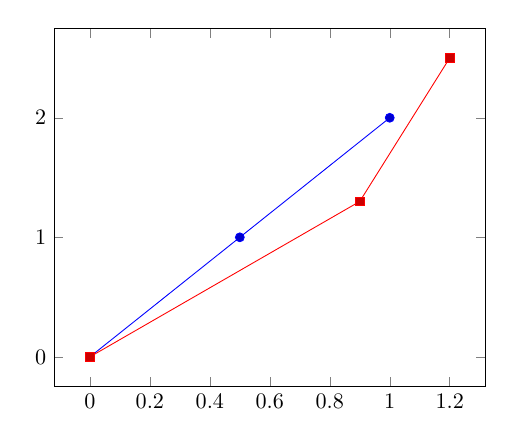
\begin{tikzpicture}[scale=0.8]
\begin{axis}
\addplot coordinates {
(0,0)
(0.5,1)
(1,2)
};
\addplot coordinates {
(0,0)
(0.9,1.3)
(1.2,2.5)
};
\end{axis}
\end{tikzpicture}
\captionsetup[figure]{format=hang, name=Fig, font=footnotesize}
\captionof{figure}{Example Chart. This chart has no legend and also has no lables to indicate what the y-axis and x-axis represent.}
\label{fig:exchart}
\medskip


For example the chart shown in figure \ref{fig:exchart} has been typeset within a multicolumns environment and has utilized the space around it effectively. However it suffers from other short-comings. 

A figure, much like a table, has to be self-contained. No detail (symbol, line, etc.) of the figure should go undefined. In cases in which symbol
identifications are too long to be included in the data field, they are
included in the figure legend. Figure legends consist of figure numbers
and titles. The figure legend should briefly report what is in the graph,
not discuss the methods or meaning of the data. For reasons unknown
to me, it is customary for figure legends to be set below the graph;3
in contrast, you will recall that legends for tables are set on top of the
tables. \cite{ivan2001}

One should also consider the absence of axes, where they t represent.
\includegraphics[width=\linewidth]{math-tikz.pdf}
\end{multicols}


\section{The bullet graph}

The bullet graph is considered\footnote{\protect\url{http://www.perceptualedge.com/blog/?p=375}} to be a  better alternative to gauges in dashboards. A solution to a basic chart can be found at tx.se\footnote{\url{http://tex.stackexchange.com/questions/117314/is-there-any-package-to-create-bullet-gauge-graphs}}, by Jake, which sadly in a community of mathematicians, engineers and programmers was not popularized to the extend it deserved. 

Bullet gauges are commonly used to show the current state relative to a reference value with a background that divides the scale into regions.

\begin{figure}[htbp]
\centering

\includegraphics{./images/bullet-graph.png}
\caption{Bullet graph with annotations, indicating the various components of the graph.}
\end{figure}



current sales --
previous sales --
good -- 
great -- last shade box

Formatting: The color is preferable to be a range of distinct hues, which can also assist by those who are colorblind. It is also reproduced better when photocopies.  Intensities are preferred as follows:

three: 40\%, 25\% and 10\%

\makeatletter
\newenvironment {bulletgraph} {\luacode@begin\luacode@table@soft} {}
\makeatother

\pgfplotscreateplotcyclelist{bullet}{
{fill=color1, draw=none},
{fill=color2, draw=none},
{fill=color3, draw=none},
}

\pgfplotsset{mark options/.style={color=black!80}}
\pgfplotsset{barwidth/.style= {bar width=1.2ex} }
\pgfplotsset{chartheight/.style ={height=#1}}

\providecommand{\bulletgauge}[4][]{
    \begin{tikzpicture}[scale=0.8, font=\arial]
    \begin{axis}[
       width=8cm,
       chartheight = 60pt,
      % height=60pt,
       %y=2ex,
       xtick pos=left, 
       xtick = {0,50,...,400, 450},
       ytick=\empty,
       xmin=50, xmax=450,
        %enlarge y limits={abs=0ex},
        tick align=outside,
        axis on top,
        every axis title/.style={
            at={(rel axis cs:0,0.5)},
            anchor=east,
            align=right,
            xshift=-0.5em
        },
        #1
    ]
    \pgfplotsinvokeforeach{#4}{
        \pgfplotsset{cycle list name=bullet}
        \addplot +[xbar, bar width=7ex ] coordinates {(##1,0)};
    }
    \addplot [fill= barcolour, xbar, barwidth ] coordinates {(#2,0)};    
    \addplot [mark=|, mark options={very thick}, mark size=2ex, ] coordinates {(#3,0)}; 
    \end{axis}
    \end{tikzpicture}
}

\begin{scriptexample}{}{}
\begin{bulletgraph}
  m = require("i18n.bulletgraph")
 local data = {
     title = 'Valuation (Jan)',
     ranges = {230,300,500},
     bar = 200,
     marker = 220}
     local options = {
        barcolour = 'red!90'
   } 
m:render(data,options)        
\end{bulletgraph}
\medskip

\begin{bulletgraph}
   m = require("i18n.bulletgraph")
   local data = {
      title = 'Valuation (Apr)',
      ranges = {200,300,500},
      bar = 250,
      marker = 300}
   -- render the plot
   m:render(data,options)           
\end{bulletgraph}
\end{scriptexample}

Use an updated pgfplotsversion as we use |\pgfplotsset{compat=1.11}|, when we load the \pkgname{phd}. The environment |\begin{bulletgraph}|  is a |\luacode|  based environment and hence all the code has to be in lua syntax.

The code load the lua module |bulletgraph| and we the graph is rendered using the method \luacmd{render()}. The method, like most of the plotting routines provided by the package takes two arguments |data| and |options|.

\begin{texexample}{Bullet Plots}{ex:bulletplot}
\begin{bulletgraph}
local  bgraph = require("i18n.bulletgraph")
local data = {
     title = 'Valuation (Jan)',
     ranges = {230,300,500},
     bar = 200,
     marker = 220}
local options = {
        barcolour = 'red!90'
   } 
bgraph:render(data,options)        
\end{bulletgraph}
\end{texexample}

If you are familiar with Javascript you must have come across jQuery and its many plugins. The bulletgraph methods work in a similar fashion, where the options are a set of key values, that are used as a mixin with a set of default key values. If you only want to change the color of the bar, you only specify the color in the options the rest
are inherited from default values. All the \pkgname{phd} package routines, follow this design pattern to simplify the user interface and to enable typographical styles to be maintained throughout a publication. The best way to draw such charts is without the |options|. This separation of the interface, it also separates the data from the presentational aspects of drawing the plots.

\begin{texexample}{Bullet Plots (without options)}{ex:bulletplot1}
\begin{bulletgraph}
local  bgraph = require("i18n.bulletgraph")
local data = {
     title = 'Valuation (Jan)',
     ranges = {230,300,500},
     bar = 200,
     marker = 220}
bgraph:render(data,options)        
\end{bulletgraph}
\end{texexample}

\section{Using matplotlib}

Many researchers use Python to produce charts. A good guide can be found at \href{https://github.com/jbmouret/matplotlib_for_papers}{jbmournet} at github. There was also a good discussion at HN\footnote{\protect\url{https://news.ycombinator.com/item?id=9043571}}.












% %\bgroup
\arial


\chapter{South Asian Scripts}

The scripts of South Asia share so many characteristics that a side by side comparison of a few often reveal structural similarities even in the 
modern letterforms.
\medskip


\begin{center}
\begin{tabular}{lll}
  \hyperref[s:devanagari]{Devanagari} 
& \hyperref[s:gujarati]{Gujarati}
& \hyperref[s:telugu]{Telugu}\\
  \hyperref[s:bengali]{Bengali}
& \hyperref[s:oriya]{Oriya} 
& \hyperref[s:kannada]{Kannada}\\
  \hyperref[s:gurmukhi]{Gurmukhi} 
& \hyperref[s:tamil]{Tamil}
& \hyperref[s:malayalam]{Malayalam}\\
  \hyperref[s:sinhala]{Sinhala} 
& \hyperref[s:kaithi]{Kaithi}  
& \hyperref[s:meeteimayek]{Meetei Mayek}\\
  \hyperref[s:tibetan]{Tibetan} 
& \hyperref[s:saurashtra]{Saurashtra} 
& \hyperref[olchiki]{Ol Chiki}\\
  \hyperref[s:lepcha]{Lepcha}
& \hyperref[s:sharada]{Sharada} 
& \hyperref[s:sorasompeng]{Sora Sompeng}\\
  \hyperref[s:phagspa]{Phags-pa} 
& \hyperref[s:takri]{Takri}  
& \hyperref[s:kharoshthi]{Kharoshthi}\\
  \hyperref[s:limbu]{Limbu} 
& \hyperref[s:chakma]{Chakma}
& \hyperref[s:brahmi]{Brahmi}\\
  \hyperref[s:sylotinagra]{Syloti Nagri} 
& \hyperref[s:mro]{Mro} 
&\\
\end{tabular}
\end{center}

The sections that follow describe the scripts briefly and the |phd| settings
to activate the relevant commands and load appropriate fonts. 

\begin{figure}[htbp]
\includegraphics[width=\textwidth]{./images/indic-language-tree.jpg}
\caption{A family tree of a few of the most important Indic scripts, (adapted from \protect\cite{writing}.}
\end{figure}


\section{Sinhala Alphabet}
\label{s:sinhala}
\index{scripts>Sinhala}

The Sinhala alphabet derives from Pali.

\newfontfamily{\sinhala}{NotoSansSinhala-Regular.ttf}

\begin{docKey}[phd]{sinhala font}{ = \meta{font face}}{default none, initial NotoSansSinhala-Regular.ttf}
\end{docKey}

\begin{docCommand}{textsinhala}{\marg{text}}
Command to typeset sinhalese text.
\end{docCommand}

\begin{docEnvironment}{sinhalascript}{}{}
\end{docEnvironment}

The \refEnv{sinhalascript} environment typesets text inputted in the Sinhala script.

\begin{scriptexample}[]{Sinhala}
\unicodetable{sinhala}{"0D80,"0D90,"0DA0,"0DB0,"0DC0,"0DD0,"0DE0,"0DF0}
\end{scriptexample}

\printunicodeblock{./languages/sinhala.txt}{\sinhala}
\section{Meitei Mayek alphabet}
\label{s:meiteimayek}
\index{scripts>Meitei Mayek}
\index{Meetei Mayek}
\newfontfamily\meitei{Noto Sans Meetei Mayek}

\def\textmeitei#1{{\meitei #1}\xspace}

Meithei (Meitei) /ˈmeɪteɪ/,[4] also known as Manipuri /mænɨˈpʊəri/ ({\pan মৈতৈলোন্} \textmeitei{ꯃꯧꯇꯧꯂꯣꯟ} Meitei-lon or {\pan মৈতৈলোল্} \textmeitei{ꯃꯧꯇꯧꯂꯣꯜ} Meitei-lol), is the predominant language and lingua franca in the southeastern Himalayan state of Manipur, in northeastern India. It is the official language in government offices. Meithei is also spoken in the Indian states of Assam and Tripura, and in Bangladesh and Burma (now Myanmar).

The Meitei (also Meetei, Meithei, Manipuri) people are the majority ethnic group of Manipur, a northeastern state of India. Meitei is an endonym or autonym while Manipuri is an exonym. A significant population of the Meitei also are settled in domestic neighboring states such as Assam[1] and Tripura. They have also settled in Bangladesh[2] and Myanmar.[3]
The Meitei people are made up of seven major clans known as Salai Taret.[4] Their written history has been documented to 1445 BC.[5]

Meithei is a Tibeto-Burman language whose exact classification remains unclear, though it shows lexical resemblances to Kuki and Tangkhul Naga.[5] The language is spoken by more than 1.5 million people.

\begin{figure}[htbp]
\centering
\includegraphics[width=\linewidth]{dancing}

\caption{"Khamba-Thoibi" Jagoi 
RKCS paintings on the walls of temple of Ibudhou Thangjing at Moirang, Manipur. 
Picture Courtesy - Recky Maibram.}
\end{figure}

Meithei has proven to be an integrating factor among all ethnic groups in Manipur who use it to communicate among themselves. It has been recognized (as Manipuri), by the Indian Union and has been included in the list of scheduled languages (included in the 8th schedule by the 71st amendment of the constitution in 1992). Meithei is taught as a subject up to the post-graduate level (Ph.D.) in universities of India, apart from being a medium of instruction up to the undergraduate level in Manipur.

\bgroup
\meitei
\begin{tabular}{>{\arial}l
                >{\arial}l
                >{\meitei}l
                >{\arial}l
                >{\arial}l
                >{\meitei}l
               }
1	&ama 	 &ꯑꯃ	       &11	&taramathoi	&\\
2	&ani	   &ꯑꯅꯤ	&12	 &taranithoi	&ky \\
3	&ahum	&ꯑꯍꯨꯝ	   &13	 &tarahumdoi	&ꯇꯔꯥꯍꯨꯝꯗꯣꯢ\\
4	&mari	&ꯃꯔꯤ	   &14  &	taramari	&ꯇꯔꯥꯃꯔꯤ\\
5	&manga	 &ꯃꯉꯥ	   &15	 &taramanga	&ꯇꯔꯥꯃꯉꯥ\\
6	&taruk	 &ꯇꯔꯨꯛ	   &16	 &tarataruk	&ꯇꯔꯥꯇꯔꯨꯛ\\
7	&taret	 &ꯇꯔꯦꯠ	   &17	 &tarataret	&ꯇꯔꯥꯇꯔꯦꯠ\\
8	&nipan &ꯅꯤꯄꯥꯟ	&18	 &taranipan	&ꯇꯔꯥꯅꯤꯄꯥꯟ\\
9	&mapan	 &ꯃꯥꯄꯟ	   &19	 &taramapan	&ꯇꯔꯥꯃꯥꯄꯟ\\
10	&tara	 &ꯇꯔꯥ	   &20	 &kun	&ꯀꯨꯟ\\
\end{tabular}
\egroup





Meitei Mayek script was added to the Unicode Standard in October, 2009 with the release of version 5.2.\index{Meitei Mayek}

The Unicode block for Meitei Mayek, called Meetei Mayek, is \unicodenumber{U+ABC0–U+ABFF}.

Characters for historical orthographies are part of the Meetei Mayek Extensions block at \unicodenumber{U+AAE0–U+AAFF}.

\begin{scriptexample}[]{Meitei}
\unicodetable{meitei}{"ABC0,"ABCD0,"ABE0,"ABF0}
\end{scriptexample}

\begin{scriptexample}[]{Meitei}
\unicodetable{meitei}{"AAE0,"AAF0}
\captionof{table}{Meetei Mayek Extensions}
\end{scriptexample}


\printunicodeblock{./languages/meetei-mayek.txt}{\meitei}


% http://e-pao.net/eyek/tamba/




%\section{Tibetan}
\label{tibetan}
\index{scripts>tibetan}


Another important Northern Indian member perhaps
derived directly from Gupta---and thus a sister script to Nagari,
Sarada and Pali---is Tibetan. However, the Tibetan
language wears this foreign Indo-Aryan script most uncomfortably.\cite{writing}
The script retains the Indic consonantal alphabet with diacritic
attachments to indicate vowels – but with only one vowel
letter, the /a/, which is the same as the system’s own ‘default’ /a/.
This /a/ letter is then used to attach other diacritics in order to
indicate further vowels. Because the Tibetan language has
changed greatly since c. AD 700 (when the script was first elaborated
from Gupta) while the script has remained almost
unchanged, Tibetan is extremely difficult to read today. Its
greatest problem is that it marks none of the tones of its tonal
language. Though Tibetans have long tried to adapt written
Tibetan to spoken Tibetan, high illiteracy has been the price of
failing to achieve this. Tibetan schools in Tibet, by governmental
decree, now teach only the Chinese script and in the Chinese
language.

\newfontfamily\tibetan{TibMachUni.ttf}

\newfontfamily\tibetan{Qomolangma-Chuyig.ttf}

%A should pick it up automatically \tibetan

Fonts described in this section can be obtained from The Tibetan \& Himalayan Library
\footnote{\url{http://www.thlib.org/tools/scripts/wiki/tibetan\%20machine\%20uni.html}  }

I have tried a few \texttt{Tibetan Machine Uni (TMU)} seems to be used by a number of scholars. 

A tip when you are trying to locate fonts is to find a related article in Wikipedia, such as Tibetan alphabet and inspect the element using your browser to see what fonts are being used.


|style="font-family:'Jomolhari','Tibetan Machine Uni','DDC Uchen', 'Kailash';| 


If you cannot see the script and rather than boxes or question marks then you can search and download one of the fonts in |font-family|.



\begin{docKey}[phd]{language}{ = tibetan}{default none, initial english} 
The key |language=tibetan| sets the default language as Tibetan, using the main font given by the key |tibetan font=TibMachUni.ttf|.

It will also create an environment tibetanlanguage.
\end{docKey}

\begin{docKey}[phd]{tibetan font}{= TibMachUni.ttf} {initial = TibMachUni.ttf} 
The key |tibetan font=font-name| sets the default font for the Tibetan language. It will also create the switch \cmd{\tibetan} for typesetting text in Tibetan.
\end{docKey}


\begin{docEnvironment}{tibetan}{}
\end{docEnvironment}

The environment is created automatically
\begin{texexample}{Tibetan language setttings}{ex:tibetan}
\bgroup
\cxset{language=tibetan, tibetan font = TibMachUni.ttf}

\tibetan Tibetan: དབུ་ཅན\par
ཨོཾ་ཨཿཧཱུྂ་བཛྲ་གུ་རུ་པདྨ་སིདྡྷི་ཧཱུྂ༔\par
\egroup

\begin{tibetanlanguage}
The tibetan environment\par
ཨོཾ་ཨཿཧཱུྂ་བཛྲ་གུ་རུ་པདྨ་སིདྡྷི་ཧཱུྂ༔
\end{tibetanlanguage}
\end{texexample}


The Tibetan alphabet is an \emph{abugida} of Indic origin used to write the Tibetan language as well as Dzongkha\footnote{Spoken in Bhutan.}, the Sikkimese language, Ladakhi, and sometimes Balti. 

The printed form of the alphabet is called \textit{uchen} script (Tibetan: དབུ་ཅན་, Wylie: dbu-can; "with a head") while the hand-written cursive form used in everyday writing is called umê script (Tibetan: དབུ་མེད་, Wylie: dbu-med; "headless").

The alphabet is very closely linked to a broad ethnic Tibetan identity. Besides Tibet, it has also been used for Tibetan languages in Bhutan, India, Nepal, and Pakistan.[1] The Tibetan alphabet is ancestral to the Limbu alphabet, the Lepcha alphabet,[2] and the multilingual 'Phags-pa script.[2]


The Tibetan alphabet is romanized in a variety of ways.[3] This article employs the Wylie transliteration system.

The Tibetan alphabet has thirty basic letters, sometimes known as "radicals", for consonants.[2]

{\tibetanfontfamily
ཀ ka /ká/	ཁ kha /kʰá/	ག ga /kà, kʰà/	ང nga /ŋà/\\
ཅ ca /tʃá/	ཆ cha /tʃʰá/	ཇ ja /tʃà/	ཉ nya /ɲà/\\
ཏ ta /tá/	ཐ tha /tʰá/	ད da /tà, tʰà/	ན na /nà/\\
པ pa /pá/	ཕ pha /pʰá/	བ ba /pà, pʰà/	མ ma /mà/\\
ཙ tsa /tsá/	ཚ tsha /tsʰá/	ཛ dza /tsà/	ཝ wa /wà/ (not originally part of the alphabet)[5]\\
ཞ zha /ʃà/[6]	ཟ za /sà/	འ 'a /hà/[7]\\
ཡ ya /jà/	ར ra /rà/	ལ la /là/\\
ཤ sha /ʃá/[6]	ས sa /sá/	ཧ ha /há/[8]\\
ཨ a /á/\\
}


Tibetan is not a difficult script to read or write, but it is a very complex script to deal with in terms of computer processing (as far as complexity goes I would rate it second only to the Mongolian script). The problem is that written Tibetan comprises complex syllable units (known in Tibetan as a tsheg bar {\tibetan ཚེག་བར}) which although written horizontally may include \emph{vertical} clusters of consonants and vowel signs agglutinating around a base consonant (a vertical cluster is known as a "stack"). 

Thus most words have a horizontal and a vertical dimension, with the result that text is not laid out in a straight line as in most scripts. For example, the word bsGrogs བསྒྲོགས་ (pronounced drok ... obviously!) may be analysed as follows :

\definecolor{lavenderblush}{HTML}{FFF0F5}%
\definecolor{beige}{HTML}{F5F5DC}%


{\tibetan 
\HUGE བསྒྲོགས

{\color{beige}%
\symbol{"0F56}\color{blue!40}\color{red}\symbol{"0F66}\symbol{"0F92}\color{blue!80}\symbol{"0FB2}\color{beige}\symbol{"0F7C}\color{blue!25}\symbol{"0F42}\symbol{"0F66}\symbol{"0F0B}}



\begin{tabular}{|l|}
\symbol{"0F56}\symbol{"0F7C}\\
\symbol{"0F42}\symbol{"0F7C}\\
\symbol{"0F66}\symbol{"0F7C}\\
\symbol{"0F40}\symbol{"0F7C}\\
\end{tabular}
}

\subsection{Unicode Block Tibetan}


\bgroup\large\tibetan
\begin{tabular}{llllllllllllllll l}
\toprule
	           &|0|	&|1|	&|2|	&|3|	&|4|	&|5|	&|6|	&|7|	&|8|	&|9|	&|A|	&|B|	&|C|	&|D|	&|E|	&|F|\\
\midrule
\texttt{U+0F0x}	&ༀ	&༁	&༂	&༃	&༄	&༅	&༆	&༇	&༈	&༉	&༊	&་	&༌  &	།	&༎	&༏\\
\midrule
\texttt{U+0F1x} &༐	&༑	&༒	&༓	&༔	&༕	&༖	&༗	&༘&	༙	&༚	&༛	&༜	&༝	&༞	&༟\\
\midrule
\texttt{U+0F2x} &༠	&༡	&༢	&༣	&༤	&༥	&༦	&༧	&༨	&༩	&༪	&༫	&༬	&༭	&༮	&༯\\
\midrule
\texttt{U+0F3x}	&༰ &༱	 &༲ &༳	&༴ &༵	&༶ & ༷	&༸&	༹	&༺&	༻	&༼&	༽	&༾	&༿\\
\midrule
\texttt{U+0F4x} &ཀ	&ཁ	&ག	&གྷ	&ང	&ཅ	&ཆ	&ཇ	&	&ཉ	&ཊ	&ཋ	&ཌ	&ཌྷ	&ཎ	&ཏ\\
\midrule
\texttt{U+0F5x}	 &ཐ	&ད	&དྷ	&ན	&པ	&ཕ	&བ	&བྷ	&མ	&ཙ	&ཚ	&ཛ	&ཛྷ	&ཝ	&ཞ	&ཟ\\
\midrule
\texttt{U+0F6x} &འ	&ཡ	&ར	&ལ	&ཤ	&ཥ	&ས	&ཧ	&ཨ	&ཀྵ	&ཪ	&ཫ	&ཬ	&&&\\
^^A\texttt{U+0F7x}&&	ཱ &	& &ི	ཱི&	ུ&	ཱུ&	ྲྀ&	ཷ&	ླྀ&	ཹ&	ེ&	ཻ&	ོ&	ཽ&	&ཾ	&ཿ\\
\midrule
\texttt{U+0F8x}&    ྀ   & 	ཱྀ&	ྂ&	&ྃ &	྄	&྅&	྆	&྇	ྈ&	ྉ&	ྊ&	ྋ&	ྌ&	ྍ&	ྎ&	ྏ\\
\midrule
\texttt{U+0F9x} &	ྐ&	ྑ   & 	ྒ &	ྒྷ &	ྔ &	ྕ &	ྖ &	ྗ &		ྙ &	ྚ &	ྛ &	ྜ &	ྜྷ &	ྞ &	ྟ\\
\texttt{U+0FAx} &	ྠ &	ྡ &	ྡྷ &	ྣ &	ྤ &	ྥ &		&ྦ	&ྦྷ	ྨ&	ྩ&	ྪ&	ྫ&	ྫྷ&	ྭ&	ྮ&	ྯ\\
\midrule
\texttt{U+0FBx} 
&	  ྰ 
&	
& ྱ  	 
&ྲ	
&ླ	
&ྴ
&	ྵ
&	ྶ
&	ྷ
&ྸ
&
&
&
&	
&྾	
&྿\\
\midrule
\texttt{U+0FCx}	 &࿀&	࿁&	࿂&	࿃&	࿄&	࿅&	&࿇	&࿈	&࿉	&࿊	&࿋	&࿌	&&	࿎	&࿏\\
\midrule
\texttt{U+0FDx}	&࿐	&࿑	&࿒	&࿓	&࿔	&࿕	&࿖	&࿗	&࿘	&࿙	&࿚	&&&&&\\
\midrule
\texttt{U+0FEx} &&&&&&&&&&&&&&&&\\
\midrule
\texttt{U+0FFx}  &&&&&&&&&&&&&&&&\\
\bottomrule
\end{tabular}
\egroup




\subsection{Fonts for Tibetan}

Fonts for Tibetan need to be downloaded one set of fonts are the \texttt{Qomolangma}. They come in different flavours, but they appear
to offer advantages as compared to the Tibetan Machine Uni.
\medskip


\newfontfamily\betsu{Qomolangma-Betsu.ttf}
\newfontfamily\drutsa{Qomolangma-Drutsa.ttf}
\newfontfamily\chuyig{Qomolangma-Chuyig.ttf}
\newfontfamily\tsumachu{Qomolangma-Tsumachu.ttf}
\newfontfamily\uchensutung{Qomolangma-UchenSutung.ttf}
\newfontfamily\uchensuring{Qomolangma-UchenSuring.ttf}
\newfontfamily\uchensarchen{Qomolangma-UchenSarchen.ttf}
\newfontfamily\uchensarchung{Qomolangma-UchenSarchung.ttf}
\newfontfamily\tsuring{Qomolangma-Tsuring.ttf}
\newfontfamily\TMU{TibMachUni.ttf}
\newfontfamily\himalaya{Microsoft Himalaya}


{
\centering

\renewcommand{\arraystretch}{1.5}

\begin{tabular}{lr}
\toprule
|Qomolangma-Betsu.ttf| & {\betsu  དབུ་མེད }\\
\midrule
|Qomolangma-Chuyig.ttf| &{\chuyig  དབུ་མེད}\\
\midrule
|Qomolangma-Drutsa.ttf| &{\drutsa  དབུ་མེད}\\
\midrule
|Qomolangma-Tsumachu.ttf|&{\tsumachu  དབུ་མེད}\\
\midrule
|Qomolangma-Tsuring.ttf| &{\tsuring  དབུ་མེད}\\
\midrule
|Qomolangma-UchenSarchen.ttf| &{\uchensarchen དབུ་མེད}\\
\midrule
|Qomolangma-UchenSarchung.ttf|&{\uchensarchung དབུ་མེད }\\
\midrule
|Qomolangma-UchenSuring.ttf|&{\uchensuring དབུ་མེད}\\
\midrule
|Qomolangma-UchenSutung.ttf|&{\uchensutung དབུ་མེད }\\
\midrule
|TibMachUni.ttf| &{\TMU དབུ་མེད }\\
\midrule
|Microsoft Himalaya| &{\himalaya དབུ་མེད ཽ}\\
\bottomrule
\end{tabular}

}
\bigskip

\bgroup
\LARGE\tsuring
\noindent༆ །ཨ་ཡིག་དཀར་མཛེས་ལས་འཁྲུངས་ཤེས་བློ  འི་\par
གཏེར༑ །ཕས་རྒོལ་ཝ་སྐྱེས་ཟིལ་གནོན་གདོང་ལྔ་བཞིན།།\par
ཆགས་ཐོགས་ཀུན་བྲལ་མཚུངས་མེད་འཇམ་དབྱངསམཐུས།།\par
མཧཱ་མཁས་པའི་གཙོ་བོ་ཉིད་འགྱུར་ཅིག། །མངྒལཾ༎\par
བསྒྲོགས
\egroup

\subsubsection{Tibetan numbers}
\cxset{language=tibetan, tibetan font = TibMachUni.ttf}

{
\obeylines
\small
TIBETAN DIGIT ZERO\tibetan	༠
TIBETAN DIGIT ONE	\tibetan༡	
TIBETAN DIGIT TWO\tibetan	༢	
TIBETAN DIGIT THREE\tibetan	༣	
TIBETAN DIGIT FOUR	\tibetan ༤	
TIBETAN DIGIT FIVE\tibetan	༥	
TIBETAN DIGIT SIX	\tibetan ༦	
TIBETAN DIGIT SEVEN\tibetan	༧	
TIBETAN DIGIT EIGHT\tibetan	༨	
TIBETAN DIGIT NINE\tibetan	༩	
TIBETAN DIGIT HALF ONE	\tibetan༪	
TIBETAN DIGIT HALF TWO	༫	
TIBETAN DIGIT HALF THREE	༬
TIBETAN DIGIT HALF FOUR ༭	
TIBETAN DIGIT HALF FIVE ༯	
TIBETAN DIGIT HALF SIX	 ༯	
TIBETAN DIGIT HALF SEVEN	༰	
TIBETAN DIGIT HALF EIGHT	༱	
TIBETAN DIGIT HALF NINE	༲	
TIBETAN DIGIT HALF ZERO	༳	
}


Tibetan numbers

The usage is not certain. By some interpretations, this has the value of 9.5. Used only in some traditional contexts, these appear as the last digit of a multidigit number, eg. ༤༬ represents 42.5. These are very rarely used, however, and other uses have been postulated.


\PrintUnicodeBlock{./languages/tibetan.txt}{\himalaya}


\section{Oriya}
\label{s:oriya}
\index{Indic scripts>Oriya}
\epigraph{Oṛiyā is encumbered with the drawback of an excessively awkward and cumbrous written character. ... At first glance, an Oṛiyā book seems to be all curves, and it takes a second look to notice that there is something inside each.}{(G. A. Grierson, \textit{Linguistic Survey of India}, 1903)}

\newfontfamily\oriya[Scale=1.1,Script=Oriya]{Noto Sans Oriya}

\def\oriyatext#1{{\oriya#1}}
The Oriya script or Utkala Lipi (Oriya: \oriyatext{ଉତ୍କଳ ଲିପି}) or Utkalakshara (Oriya: \oriyatext{ଉତ୍କଳାକ୍ଷର}) is used to write the Oriya language, and can be used for several other Indian languages, for example, Sanskrit.

\centerline{\Huge\oriyatext{ଉତ୍କଳ ଲିପି}}

\bgroup
\oriya
୦୧୨୩୪୫୬୭୮୯
ଅ ଆ ଇ ଈ ଉ ଊ ଋ ୠ ଌ ୡ ଏ ଐ ଓ ଔ କ ଖ ଗ ଘ ଙ ଚ ଛ ଜ ଝ ଞ ଟ ଠ ଡ ଢ ଣ ତ ଥ ଦ ଧ ନ ପ ଫ ବ ଵ ଭ ମ ଯ ର ଳ ୱ ଶ ଷ ସ ହ ୟ ଲ
\egroup






\begin{figure}[htbp]
\centering

\includegraphics[width=\linewidth-2\parindent]{oriya-people}

\hspace*{-1em}\caption{Children dressed for celebration of Janmashtami, which marks the birth of Lord Krishna. odisha360.com}
\end{figure}

Comparison of Oṛiyā script with its neighbours

At a first look the great number of signs with round shapes suggests a closer relation to the southern neighbour Telugu than to the other neighbours Bengali in the north and Devanāgarī in the west. The reason for the round shapes in Oriya and Telugu (and also in Kannaḍa and Malayāḷam) is the former method of writing using a stylus to scratch the signs into a palm leaf. These tools do not allow for horizontal strokes because that would damage the leaf.

Oriya letters are mostly round shaped whereas in Devanāgarī and Bengali have horizontal lines. So in most cases the reader of Oṛiyā will find the distinctive parts of a letter only below the hoop. Considering this the  closer relation to Devanāgarī and Bengali exists than to any southern script, though both northern and southern scripts have the same origin, Brāhmī.

Oriya (\oriyatext{ଓଡ଼ିଆ} oṛiā), officially spelled Odia,[3][4] is an Indian language belonging to the Indo-Aryan branch of the Indo-European language family. It is the predominant language of the Indian states of Odisha, where native speakers comprise 80\% of the population,[5] and it is spoken in parts of West Bengal, Jharkhand, Chhattisgarh and Andhra Pradesh. Oriya is one of the many official languages in India; it is the official language of Odisha and the second official language of Jharkhand. [6][7][8] Oriya is the sixth Indian language to be designated a Classical Language in India, on the basis of having a long literary history and not having borrowed extensively from other languages.



\printunicodeblock{./languages/oriya.txt}{\oriya}

\section{Numerals}

{\oriya
\obeylines
୦	୧	୨	୩	୪	୫	୬	୭	୮	୯	୵	୶	୷	୲	୳	୴
{\arial 0	1	2	3	4	5	6	7	8	9	¹⁄₁₆	⅛	³⁄₁₆	¼	½	¾}
}




\section{Mro (Mru language)}
\label{s:mro}

\newfontfamily\mro{MroUnicode-Regular.ttf}
\def\textmro#1{{\mro #1\xspace}}

 Mro (or Mru) is a Tibeto-Burman language spoken primarily in Bangladesh with a few
speakers in India. 

Mru is a Tibeto-Burman language and one of the recognized languages of Bangladesh. It is spoken by a community of Mros (Mru) inhabiting the Chittagong Hill Tracts of Bangladesh and also in Burma with a population of 22,000 in Bangladesh according to the 1991 census. The Mros are the second-largest tribal group in Bandarban District of the Chittagong Hill Tracts. A small group of Mros also live in Rangamati Hill District.

The Mru language is considered "definitely endangered" by UNESCO in June 2010.[4]

The script was invented in the 1980s and is of the class of “messianic”
scripts with no genetic relationship with existing scripts. In the last 10 years there has been an acceptance
among all the Mro to use this script and literacy levels among the 100,000 Mro exceed 80\%.

Some of the characters of the Mro alphabet have a visual similarity to those from other alphabets, but this
relationship is purely coincidental, and the Mro alphabet stands alone as a unity.


The Mro script has no technical complexity: it is a simple left to right alphabet with no
combining characters or characters with special function. There are no tone marks. Some sounds are
represented by more than one letter. The sound [k] is usually represented by \textmro{𖩌} KEAAE kəɘ, as in \textmro{𖩌𖩑𖩗} kow
‘village’, \textmro{𖩄𖩑𖩁𖩌𖩑} boŋko ‘owl’, but in a few words the letter 𖩙 KOO ko is used, as in \textmro{𖩙𖩑} ko ‘gold’. The sound
[m] is usually represented by \textmro{𖩎} MAEM mɘm, as in \textmro{𖩎𖩆𖩁} maŋ ‘go’, \textmro{𖩔𖩎𖩑} śmo ‘fool’, but in a few words the
letter \textmro{𖩃} MIM mim is used, as in \textmro{𖩃𖩊𖩏} min ‘cat’, \textmro{𖩋𖩃𖩊} cmi ‘rice’. The sound [l] is usually represented by \textmro{𖩍} OL
\textmro{ɔl}, as in \textmro{𖩍𖩝𖩁} lɔŋ ‘boat’, \textmro{𖩈𖩍𖩆} khla ‘spoon’, but in a few words the letter \textmro{𖩛} LA la is used, as in \textmro{𖩛𖩆𖩎𖩖} lamɘ
‘moon’, and in a few words \textmro{𖩚} LAN lan is used (we have no example). The vowels \textmro{𖩑𖩖} oɘ are used as a
digraph to describe the vowel [ø].

We are using Philip Reimer's font which is freely available under SIL OFL licence at \href{http://phjamr.github.io/mro.html}{github}. Philip has also produced fonts for two other scripts: Lisu (Fraser) and Miao (Pollard). All three scripts were added to Unicode 7.0 in 2014.



\begin{scriptexample}[]{Mro}
\unicodetable{mro}{"16A40,"16A50,"16A60}
\end{scriptexample}


\printunicodeblock{./languages/mro.txt}{\mro}








\section{Devanagari}
\label{s:devanagari}
\parindent1em

Devanagari is part of the Brahmic family of scripts of India, Nepal, Tibet, and South-East Asia.[2] It is a descendant of the Gupta script, along with Siddham and Sharada.[2] Eastern variants of Gupta called nāgarī are first attested from the 7th century CE; from c. 1200 CE these gradually replaced Siddham, which survived as a vehicle for Tantric Buddhism in East Asia, and Sharada, which remained in parallel use in Kashmir. An early version of Devanagari is visible in the Kutila inscription of Bareilly dated to Vikram Samvat 1049 (i.e. 992 CE), which demonstrates the emergence of the horizontal bar to group letters belonging to a word.[3]

Sanskrit nāgarī is the feminine of nāgara \enquote{relating or belonging to a town or city}. It is feminine from its original phrasing with lipi ("script") as nāgarī lipi "script relating to a city", that is, probably from its having originated in some city.[4]

The use of the name devanāgarī is relatively recent, and the older term nāgarī is still common.[2] The rapid spread of the term Devanāgarī may be related to the almost exclusive use of this script to publish Sanskrit texts in print since the 1870s.[2]

In time, Devanagari became India’s principal script. It also
became one of the world’s most important, as it was used to
convey many other languages of the region, such as Hindi, Nepali, Marwari, 
Kumaoni and several non-Indo-Aryan
languages. Devanagari failed to become India’s sole script perhaps
because of the region’s long disunity. Subsequently, it
became the parent of, among other scripts, the Gurmukhi
which the Sikhs elaborated in the 1500s in order to write their
Punjabi language (illus. 78). Today, Devanagari survives in India
alongside some ten other major scripts (including the Latin and
Perso-Arabic alphabets) and about 190 others of lesser significance.\cite{writing}

On Windows use \texttt{Arial Unicode MS} or \texttt{Arial}
\medskip

%\newfontfamily\devanagari[Script=Devanagari,Scale=1.5]{Arial Unicode MS}
\newfontfamily\devanagarilohit[Script=Devanagari,Scale=1.1]{Lohit-Devanagari.ttf}
\let\devanagari\devanagarilohit

\begin{scriptexample}[]{Devanagari}
{\begin{center}\parindent0pt\devanagari

ंःअआइईउऊऋऌऍऎएऐऑऒओऔऔँ \par 

ी	ु	ू	ृ	ॄ	ॅ	ॆ	े	ै	ॉ	ॊ	ो	ौ	्	\par

\bigskip		
\begin{tabular}{lll lll lll l}
०	&१	&२	&३	&४	&५	&६	&७	&८	&९\\
0	&1	&2	&3	&4	&5	&6	&7	&8	&9\\
\end{tabular}
\end{center}	
}
\end{scriptexample}


On Linux \texttt{Lohit} is a font family designed to cover Indic scripts and released by Red Hat. The Lohit fonts currently cover 11 languages: Assamese, Bengali, Gujarati, Hindi, Kannada, Malayalam, Marathi, Oriya, Punjabi, Tamil, Telugu.[1] The fonts were supplied by Modular Infotech and licensed under the GPL. In September 2011, they were retroactively relicensed under the OFL.[2] The Lohit fonts are used as web fonts by some Wikimedia Foundation sites, like Wikipedia, since March 2012.The font currently support 21 Indian languages. 

\let\devanagarilohit\pan

\begin{scriptexample}[]{Devanagari}
\begin{center}\parindent0pt\devanagarilohit

ंःअआइईउऊऋऌऍऎएऐऑऒओऔऔँ \par 

ी	ु	ू	ृ	ॄ	ॅ	ॆ	े	ै	ॉ	ॊ	ो	ौ	्	\par

\bigskip		
\begin{tabular}{lll lll lll l}
०	&१	&२	&३	&४	&५	&६	&७	&८	&९\\
0	&1	&2	&3	&4	&5	&6	&7	&8	&9\\
\end{tabular}
\end{center}
\end{scriptexample}

\subsubsection{Punctuation} 
The end of a sentence or half-verse may be marked with a dot known as a pūrna virām or a vertical line danda: \textbar. The end of a full verse may be marked with two vertical lines: \textbar\textbar. A comma, or alpa virām, is used to denote a natural pause in speech. With expansion of English speakers in India, the full stop is also sometimes used.

\subsection{LaTeX support}

\latex2e support can be found in the \pkgname{sanskrit}. The package contains the font files and pre-processor for printing Sanskrit
text in both devanāgarī and transliterated Roman with diacritics. Another package that can be used with \XeTeX\ is support \pkgname{devnag}.  This was originally developed by Frans Velthuis for the University of Groningen, The Netherlands, and it was the first system to provide
support for the script for \tex. The package was  extended by Anshuman Pandey. The package provides both fonts as well as tranliteration macros.


\printunicodeblock{./languages/devanagari.txt}{\devanagarilohit}






\section{Bengali}
\label{s:bengali}
\idxlanguage{Bengali}
\index{Bengali fonts>Shonar Bangla}
\index{Bengali fonts>Vrinda}
\index{Bengali fonts>Noto Sans Bengali}
\index{Bengali fonts>Noto Serif Bengali}
\index{Bengali}
%\newfontfamily\bengali[Script=Bengali,Scale=1.3]{Shonar Bangla}
\newfontfamily\bengali[Script=Bengali,Scale=1.0]{Noto Serif Bengali}
There are two Windows fonts that can be used with Windows \textit{Shonar Bangla} and \textit{Vrinda}. For open source fonts one can use, \texttt{Not Serif Bengali}.

\docAuxCommand{bengali} and \docAuxCommand{textbengali} Once the key is set the command \cmd{\bengali} is available for use in typesetting Bengali text.

\bigskip

\bgroup



\bengali
\centering

  অ  আ ই  ঈ  উ  ঊ  ঋ  এ  ঐ\par

%\newfontfamily\bengal[Script=Bengali,Scale=3.2]{Vrinda}

\centering

  অ  আ ই  ঈ  উ  ঊ  ঋ  এ  ঐ\par




\centering

  অ  আ ই  ঈ  উ  ঊ  ঋ  এ  ঐ\par

\captionof{table}{The consonant{\protect\bengali{} ক (kô)} along with the diacritic form of the vowels {\protect\bengali{} অ, আ, ই, ঈ, উ, ঊ, ঋ, এ, ঐ, ও and ঔ} \textit{from Wikipedia}.}
\egroup

\def\indexindic#1{\index{Indic Languages>#1}\index{#1} }

|Bengali| is a Unicode block containing characters for the Bangla, Assamese, Bishnupriya Manipuri, Daphla, Garo, Hallam, Khasi, Mizo, Munda, Naga, Rian, and Santali languages. In its original incarnation, the code points U+0981..U+09CD were a direct copy of the Bengali characters A1-ED from the 1988 ISCII standard, as well as several Assamese ISCII characters in the U+09F0 column. The Devanagari, Gurmukhi, Gujarati, Oriya, Tamil, Telugu, Kannada, and Malayalam blocks were similarly all based on ISCII encodings. \index{Bengali}\index{Indic Languages>Bangla}\index{Indic Languages>Assamese}\index{Indic Languages>Bishnupriya Manipuri}\indexindic{Daphla}\indexindic{Garo}\indexindic{Hallam}\indexindic{Khasi}\indexindic{Mizo}\indexindic{Munda}
\indexindic{Naga}\indexindic{Rian}\indexindic{Santali}

\begin{scriptexample}[]{Bengal}
\unicodetable{bengali}{"0980,"0990,"09A0,"09B0,"09C0,"09D0,"09E0,"09F0}
\end{scriptexample}


\printunicodeblock{./languages/bengali.txt}{\bengali}



\bgroup
\bengali\LARGE
\char"0995 + \color{blue} \char"09BC + \color{red}\char"09AF  = \char"0995\char"09CD \char"09AF
\egroup

Noto has both a serif and a sans font \docFont{Noto Serif Bengali}

See also \url{http://www.nongnu.org/freebangfont/downloads.html} for additional fonts.










\section{Saurashtra}
\label{s:saurashtra}
\idxlanguage{Saurashtra}\idxlanguage{Sourashtra}

\index{Saurashtra fonts>code2000}
\newfontfamily\saurashtra{code2000.ttf}
\def\test{}
\cxset{saurashtra font/.code=\test}
\cxset{saurashtra font=code2000.ttf}

\begin{docKey}[phd]{saurashtra font}{ = \meta{fontname}} {default none, initial = code2000}
  This key sets the saurashtra font.
\end{docKey}

Saurashtra or Sourashtra or {\saurashtra ꢱꣃꢬꢵꢰ꣄ꢜ꣄ꢬꢵ} or Palkar or Patkar (Sanskrit: सौराष्ट्र, Tamil: சௌராட்டிரம்) is an Indo-Aryan language[3] spoken by the Saurashtrian community native to Gujarat, who migrated and settled in Southern India. Madurai in Tamil Nadu has the highest number of people belonging to this community and also remains as their cultural center.

The language is largely only in spoken form even though the language has its own script. The lack of schools teaching Saurashtra script and the language is often cited as a reason for the very few number of people who actually know to read and write in Saurashtra script. Latin, Devanagari or Tamil script is used as alternative for Saurashtra Script by many Saurashtrians.

Census of India places the language under Gujarati. Official figures show the number of speakers as 185,420 (2001 census).[4]


\begin{scriptexample}[]{Saurashtra}
\unicodetable{saurashtra}{"A880,"A890,"A8A0,"A8B0,"A8C0,"A8D0}
\end{scriptexample}


\begin{scriptexample}[]{Saurashtra}
\bgroup
\saurashtra

ꢮꢶꢯ꣄ꢮ ꢱꣃꢬꢵꢰ꣄ꢜ꣄ꢬꢪ꣄ ꢦꢡ꣄ꢬꢶꢒꢾ ꢱꢵꢡ꣄ꢡꢒꢸ ꢂꢮꢬꢾ
ꢮꣁꢭꢱ꣄ꢢꢵꢥꢪꢸꢒ꣄(ꣀꢵꢮꢾꢔꢹ ꢂꢮ꣄ꢬꢶꢫꣁ


\arial

Text: Vishwa Sourashtram \url{http://www.sourashtra.info/ghEr.htm}
\egroup
\end{scriptexample}


\printunicodeblock{./languages/saurashtra.txt}{\saurashtra}

\section{Gujarati}
\label{s:gujarati}
\idxlanguage{Gujarati}
\index{Unicode>Gujarati}
%FIXME
\index{languages>Gujarati}\index{languages>Gujǎrātī Lipi}
has its own writing system, distinct but related to several other Indian languages' writing systems, such as the one used to write Hindi. Strictly speaking, the Gujarati writing system is what is called an \emph{abugida} (and not an \textit{alphabet}), because the consonant characters all contain an inherent vowel, and other vowels are written as accents added on to the consonant characters. There are also symbols for stand-alone vowels.

The Gujarati script ({\gujarati{ગુજરાતી લિપિ }} Gujǎrātī Lipi), which like all Nāgarī writing systems is strictly speaking an abugida rather than an alphabet, is used to write the Gujarati and Kutchi languages. It is a variant of Devanāgarī script differentiated by the loss of the characteristic horizontal line running above the letters and by a small number of modifications in the remaining characters.
With a few additional characters, added for this purpose, the Gujarati script is also often used to write Sanskrit and Hindi.
Gujarati numerical digits are also different from their Devanagari counterparts.
\medskip

\bgroup
\newfontfamily\gujaratilohit[Script=Gujarati,Scale=1.5]{Lohit-Gujarati.ttf}
\gujarati

\centering

\underline{English/Hindi/Gujarati Alphabets}

\hskip-1.5cm\begin{tabular}{lllllllllllllllllllll}
A &B &bh &C &ch &chh &D &dh &E &F &G &gh &H &I &J &K &kh &L &M &N &O\\

अ &ब &भ &क &च &छ &ड/द &ध/ढ़ &इ &फ &ग &घ &ह &ई &ज &क &ख &ल &म &न/ण &ऑ\\

અ &બ &ભ &ક &ચ &છ &ડ/દ &ધ /ઢ &ઇ &ફ &ગ &ઘ &હ &ઈ &જ &ક &ખ &લ &મ &ન/ણ &ઓ\\

\end{tabular}
\egroup

\medskip

Gujarati has its own set of numeric signs (placed alongside their Hindu-Arabic [or Indo-Arabic] counterparts in the tables below), they are employed in much the same way as English;  that is to say, they are put together in the same manner in order to express larger numbers. It is quite possible to simply substitute the Gujarati numerals for the Hindu-Arabic ones.

The Gujarati words for 1-10 are as follows:
\medskip

\bgroup
\begin{center}
\gujarati
\begin{tabular}{ccl}
Arabic & Gujarati &Name\\
Numeral &Numeral  &\\
0	&૦	&mīṇḍuṃ or shunya\\
1	&૧	&ekaṛo or ek\\
2	&૨	&bagaṛo or bay\\
3	&૩	&tragaṛo or tran\\
4	&૪	&chogaṛo or chaar\\
5	&૫	&pāchaṛo or paanch\\
6	&૬	&chagaṛo or chah\\
7	&૭	&sātaṛo or sāt\\
8	&૮	&āṭhaṛo or āanth\\
9	&૯	&navaṛo or nav\\
10 &૧૦ &દસ das\\

\end{tabular}
\end{center}
\egroup

\chapter{Tamil}

\epigraph{Women live like bats or owls.\\Labour like beasts\\and die like worms\ldots}{Margaret of Newcastle, 1660, England}



\label{s:tamil}
\newfontfamily\tamil[Scale=1.0, Script=Tamil]{code2000.ttf}

\def\tamiltext#1{{\tamil#1}}

\section{Background and History}

Of all the Dravidian languages Tamil has the longest literary tradition, covering
more than two thousand years. The earliest records are cave inscriptions from
the second century \textsc{bce}; the earliest extant literary text is the grammar
Tolkāppiyam (100 \textsc{bce}), which describes the grammar and poetics of Tamil during
that period. The dating of the Tolkāppiyam is still disputed by scholars proposing dates from
5 \textsc{bce} to 600 \textsc{ce}. 

During its two-thousand-year uninterrupted history, Tamil distinguishes
three different stages: Old Tamil (300 \textsc{bce} to 700 \textsc{ce}), Middle Tamil (700
\textsc{ce} to 1600) and Modern Tamil (1600 \textsc{ce} to the present), each with distinct
grammatical characteristics.\index{Dravidian>Tamil}\index{Tamil}


\begin{figure}[htbp]
\bgroup
\parindent=0pt
\centering
\includegraphics[width=0.9\linewidth-2\parindent]{./images/old-tamil-inscription.jpg}

\caption{Mangulam Tamil Brahmi inscription at Dakshin Chithra, Chennai (wikipedia)}

\egroup
\end{figure}

The Tamil script (\tamiltext{தமிழ் அரிச்சுவடி} tamiḻ ariccuvaṭi) is an abugida script that is used by the Tamil people in India, Sri Lanka, Malaysia and elsewhere, to write the Tamil language, as well as to write the liturgical language Sanskrit, using consonants and diacritics not represented in the Tamil alphabet. Certain minority languages such as Saurashtra, Badaga, Irula, and Paniya are also written in the Tamil script. \index{Surashtra}\index{Badaga}\index{Irula}

The Tamil script has 12 vowels (\tamiltext{உயிரெழுத்து} uyireḻuttu ``soul-letters''), 18 consonants (\tamiltext{மெய்யெழுத்து} meyyeḻuttu ``body-letters").
An additional character, the āytam \tamiltext{ஃ (ஆய்தம்)},  is classified in Tamil grammar as being neither a consonant nor a vowel (\tamiltext{அலியெழுத்து} aliyeḻuttu ``the hermaphrodite letter''), though often considered as part of the vowel set (\tamiltext{உயிரெழுத்துக்கள்} uyireḻuttukkaḷ ``vowel class''). The script, however, is syllabic and not alphabetic. The complete script, therefore, consists of the thirty-one letters in their independent form, and an additional 216 combinant letters representing a total 247 combinations (\tamiltext{உயிர்மெய்யெழுத்து} uyirmeyyeḻuttu) of a consonant and a vowel, a mute consonant, or a vowel alone. These combinant letters are formed by adding a vowel marker to the consonant. Some vowels require the basic shape of the consonant to be altered in a way that is specific to that vowel. Others are written by adding a vowel-specific suffix to the consonant, yet others a prefix, and finally some vowels require adding both a prefix and a suffix to the consonant. In every case the vowel marker is different from the standalone character for the vowel.
The Tamil script is written from left to right.\index{hermaphrodite letter}


\section{Unicode}

Tamil is a Unicode block containing characters for the Tamil, Badaga, and Saurashtra languages of Tamil Nadu India, Sri Lanka, Singapore, and Malaysia. In its original incarnation, the code points U+0B02..U+0BCD were a direct copy of the Tamil characters A2-ED from the 1988 ISCII standard. The Devanagari, Bengali, Gurmukhi, Gujarati, Oriya, Telugu, Kannada, and Malayalam blocks were similarly all based on their ISCII encodings.

\begin{scriptexample}[]{Tamil}
\unicodetable{tamil}{"0B80,"0B90,"0BA0,"0BB0,"0BC0,"0BE0,"0BF0}

\hfill  Typeset with \cmd{\tamil} and \texttt{code2000.ttf}
\end{scriptexample}

\subsection{Tamil Numbers and Numerals}

Originally, Tamils did not use zero, nor did they use positional digits (having separate 
symbols for the numbers 10, 100 and 1000). Symbols for the numbers are similar to 
other Tamil letters, with some minor changes. 

For example, the number 3782 is not written as \tamiltext{௩௭௮௨} as in modern usage. Instead it 
is written as \tamiltext{௩ ௲ ௭ ௱ ௮ ௰ ௨}. This would be read as they are written as 
Three Thousands, Seven Hundreds, Eight Tens, Two; or in Tamil as 
\tamiltext{௩௲௭௱௮௰௨ž}.\footnote{https://cloud.github.com/downloads/raaman/Tamil-Numeral/tamilnumbers.html}

\subsection{Dates}

Once the script is loaded the day, month and year can be loaded using the command  \cmd{\tamildate}, which returns the |\today| formatted as per custom Tamil. 

\begin{center}
\bgroup
\tamil
\begin{tabular}{lll}
day	 &month	&year	\\

௳	&௴	      &௵	\\

u	&mee	      &wa	\\
\end{tabular}
\egroup
\end{center}


\section{Grantha}
\label{s:grantha}

Grantha is a Unicode block containing the ancient Grantha script characters of 6th to 19th century Tamil Nadu and Kerala for writing Sanskrit and Manipravalam. Battled to get it working, as I could not find an appropriate unicode font. The font would need remapping. Unfortunately this is a script with no Noto support.

\begin{figure}[htbp]
\bgroup
\parindent=0pt
\centering
\includegraphics[width=\linewidth]{./images/grantha.jpg}

\caption{An image of a palm leaf manuscript with Sanskrit written in Grantha script (wikipedia)}

\egroup
\end{figure}

\newfontfamily\grantha{e-Grantamil 7}%e-Grantamil 7

\begin{scriptexample}[\grantha]{Tamil}
\unicodetable{grantha}{"0D0,"0D1,"0D2,"1133,"1134,"1135,"1136,"1137}

\hfill  Typeset with \cmd{\grantha} and \texttt{e-Granthamil 7.ttf}
\end{scriptexample}

{
\grantha \char"11311

}

%\newfontfamily\freeserif{FreeSerif}
%
%
%\freeserif \lorem
%\begin{tabular}{lll}
%day	 &month	&year	\\
%
%௳	&௴	      &௵	\\
%
%u	&mee	      &wa	\\
%\end{tabular}



\section{Malayalam}
\label{s:malayalam}
\newfontfamily\malayam[Scale=1.1]{Lohit-Malayalam.ttf}

\def\malamtext#1{{\malayam#1}}


Malayalam is a language spoken by the native people of southwestern India (from Thuckalay to Talapady).According to the Indian census of 2011, there were 32,299,239 speakers of Malayalam in Kerala, making up 93.2\% of the total number of Malayalam speakers in India, and 96.74\% of the total population of the state. There were a further 701,673 (2.1\% of the total number) in Karnataka, 957,705 (2.7\%) in Tamil Nadu, and 406,358 (1.2\%) in Maharashtra. The number of Malayalam speakers in Lakshadweep is 51,100, which is only 0.15\% of the total number, but is as much as about 84\% of the population of Lakshadweep. In all, Malayalis made up 3.22\% of the total Indian population in 2011. Of the total 34,713,130 Malayalam speakers in India in 2011, 33,015,420 spoke the standard dialects, 19,643 spoke the Yerava dialect and 31,329 spoke non-standard regional variations like Eranadan.[37] As per the 1991 census data, 28.85\% of all Malayalam speakers in India spoke a second language and 19.64\% of the total knew three or more languages.


\includegraphics[width=\textwidth]{nangeli}
https://feminisminindia.com/2016/09/12/kerala-breast-tax-nangeli/


Large numbers of Malayalis have settled in Delhi, Bangalore, Hyderabad, Mumbai (Bombay), Pune and Chennai (Madras). A large number of Malayalis have also emigrated to the Middle East, the United States, and Europe. There were 179,860 speakers of Malayalam in the United States, according to the 2000 census, with the highest concentrations in Bergen County, New Jersey and Rockland County, New York.[38] There were 7,093 Malayalam speakers in Australia in 2006.[39] The 2001 Canadian census reported 7,070 people who listed Malayalam as their mother tongue, mainly in Toronto. The 2006 New Zealand census reported 2,139 speakers.[40] 134 Malayalam speaking households were reported in 1956 in Fiji. There is also a considerable Malayali population in the Persian Gulf regions, especially in Dubai and Doha. Recently a Keralite is elected as mayor in Loughten town of England.

The Malayalam script (Malayalam: \malamtext{മലയാളലിപി}, Malayāḷalipi, IPA: [mɐləjaːɭɐ lɪβɪ], also known as Kairali script (Malayalam: \malamtext{കൈരളീലിപി}), is a Brahmic script used commonly to write the Malayalam language—which is the principal language of the Indian state of Kerala, spoken by 35 million people in the world.[3] Like many other Indic scripts, it is an alphasyllabary (\textit{abugida}), a writing system that is partially “alphabetic” and partially syllable-based. The modern Malayalam alphabet has 15 vowel letters, 41 consonant letters, and a few other symbols. The Malayalam script is a Vattezhuttu script, which had been extended with Grantha script symbols to represent Indo-Aryan loanwords.[4] The script is also used to write several minority languages such as Paniya, Betta Kurumba, and Ravula.[5] The Malayalam language itself was historically written in several different scripts.

\begin{scriptexample}[]{Malayalam}
\centerline{\Huge\malamtext{കൈരളീലിപി}}
\end{scriptexample}
\section{Syloti Nagri}
\label{s:sylotinagri}
\newfontfamily\syloti{NotoSansSylotiNagri-Regular.ttf}
\newfontfamily\damase{damase_v.2.ttf}
\index{languages>Sylheti Nagari}

Sylheti or Syloti (i.e. "Silēṭī" Bengali: সিলেটী or "Silôṭī" Bengali: ছিলটী) is one of the Bengali dialects, primarily spoken in the Sylhet Division of northeast Bangladeshi district Moulvibazar,Sylhet,Sunamganj,Hobiganj and the Barak Valley region of southern Assam. (Although sometimes it is considered an independent language for not sharing grammatical mutual intelligibility), it is a similar language to Standard Bengali, with which it shares a high proportion of vocabulary: Spratt and Spratt (1987) report 70\% shared vocabulary, while Chalmers (1996) reports at least 80\% overlap.

Sylheti Nagari or Syloti Nagri (Silôṭi Nagôri) is the original script used for writing the Sylheti language. It is an almost extinct script, this is because the Sylheti Language itself was reduced to only dialect status after Bangladesh gained independence and because it did not make sense for a dialect to have its own script, its use was heavily discouraged. The government of the newly formed Bangladesh did so to promote a greater "Bengali" identity. This led to the informal adoption of the Eastern Nagari script also used for Bengali and Assamese. It is also known as Jalalabadi Nagri, Mosolmani Nagri, Ful Nagri etc.

Sylheti Nagari was added to the Unicode Standard in March, 2005 with the release of version 4.1.
The Unicode block for Sylheti Nagari is U+A800–U+A82F:

\begin{scriptexample}[]{Sylheti}
\unicodetable{damase}{"A800,"A810,"A820}
\end{scriptexample}


\printunicodeblock{./languages/syloti.txt}{\damase}



\section{Limbu}
\label{s:limbu}

The Limbu script is used to write the Limbu language. The Limbu script is an abugida derived from the Tibetan script. Limbu is a Tibeto-Burman language spoken mainly in Nepal,[3] significant communities in Bhutan, Sikkim, Darjeeling district, India by the Limbu community. Virtually all Limbus are bilingual in Nepali.

\newfontfamily\limbu{code2000.ttf}

According to traditional histories, the Limbu script was first invented in the late 9th century by King Sirijonga Haang, then fell out of use, to be reintroduced in the 18th century by Te-ongsi Sirijunga Xin Thebe.

To change the inherent vowel, a diacritic is added. Shown here on /k/ ({\limbu ᤁ}):
Appearance	IPA

\begin{table}[htb]
\centering
\begin{tabular}{>{\Large\bfseries\limbu}l>{\arial}l}
ᤁᤡ	&/ki/\\
ᤁᤣ	&/ke/\\
ᤁᤧ	&/kɛ/\\
ᤁᤠ	&/ka/\\
ᤁᤨ	&/kɔ/\\
ᤁᤥ	&/ko/\\
ᤁᤢ	&/ku/\\
ᤁᤤ	&/kai/\\
ᤁᤦ	&/kau/\\
\end{tabular}
\caption{Changing the inherent vowel, using a diacritic.}
\end{table}




\begin{scriptexample}[]{Limbu}
\unicodetable{limbu}{"1900,"1910,"1920,"1930,"1940}
\end{scriptexample}


\printunicodeblock{./languages/limbu.txt}{\limbu}



\section{Cham}
\label{s:cham}

The Cham alphabet is an abugida used to write Cham, an Austronesian language spoken by some 230,000 Cham people in Vietnam and Cambodia. It is written horizontally left to right, as is English.

\newfontfamily\cham{Noto Sans Cham}

Cham is a Unicode block containing characters for writing the Cham language, primarily used for the Eastern dialect in Cambodia.
Cham script was added to the Unicode Standard in April, 2008 with the release of version 5.1.
The Unicode block for Cham is \textsc{U+AA00–U+AA5F}:

\begin{scriptexample}[]{Cham}
\unicodetable{cham}{"AA10,"AA20,"AA30,"AA40,"AA50}
\end{scriptexample}


\printunicodeblock{./languages/cham.txt}{\cham}


\section{Sora Sompeng}
\label{s:sorasompeng}
The Sora Language is part of the Austroasiatic language family. More locally, however, it is a part of the \hyperref[s:munda]{Munda} Languages which include other tribal languages in close proximity to Sora. Sora is unique because although it is surrounded by the Indo-Aryan language \hyperref[s:oriya]{Oriya} and the Dravidian Language Telugu, Sora is more closely related to the languages of Southeast Asia such as Khmer in Cambodia than it is to the predominant languages of India. Moreover, Sora contains very little formal literature but has an abundance of folk tales and traditions. Most of their passed down knowledge is of the oral tradition. Compared to other languages in the Munda family, Sora is decreasing within the Sora tribe at a faster rate. Most speakers are concentrated in Odisha and Andhra Pradesh but smaller communities also exist in Madhya Pradesh, Tamil Nadu, and Bihar.

Sorang Sompeng script is used to write in Sora, a Munda language with 300,000 speakers in India. The script was created by Mangei Gomango in 1936 and is used in religious contexts.[1] He was familiar with Oriya, Telugu and English, so the parent systems of the script are Brahmi and Latin.[2]
The Sora language is also written in the Latin alphabet and the Telugu script.

Sorang Sompeng script was added to the Unicode Standard in January, 2012 with the release of version 6.1. In Windows Nirmala UI.ttf (Windows 10.0) can be used. 

\newfontfamily\NirmalaU{Nirmala UI}


\unicodetable{NirmalaU}{"110D0,"110E0,"110F0}
 	

The Sora Bible employs a Latin-based orthography with a number of Sora-specific
conventions. Sora has also been rendered in the Oriya script in Orissa and in
the Telugu script in Andhra Pradesh, as well as a modified phonetic alphabet in
Ramamurti’s grammatical materials and dictionary. The use of and knowledge of
Sorang Sompeng (N. Zide 1996), the indigenous script, appears to be quite limited.
In many areas Sora remains a vital and thriving language, but one that has no state
or institutional support (sermons and materials are increasingly in Oriya in Gajapati
district which we observed and were told about in Christianized Sora communities).
In other areas, Sora is reportedly being or indeed has already been replaced by Telugu
or Oriya. So, although not an endangered language in sensu stricto, Sora (except in


\section{Numerals}\label{s:munda}

The Sora are unique in their numeral system. Instead of base 10, Sora uses a base 12 system. Only a few other languages in the world share this anomaly. Ekari, for example, uses a base 60 system.[7] For example, 39 in Sora arithmetic would be thought of as (1 * 20)+ 12 + 7. Here are the first 12 numerals in the Sora language :[7]
English: one two three four five six seven eight nine ten eleven twelve

Sora: aboy bago yagi unji monloy tudru gulji thamji tinji gelji gelmuy migel
Similar to how English uses the suffix from the numeral ten after twelve (such as thirteen, fourteen, etc.), Sora also uses a suffix assignment to numerals after 12 and before 20. Thirteen in Sora is expressed as migelboy (12+1), fourteen as migelbagu (12+2), etc.[7] Between numerals 20 and 99, Sora adds the suffix kuri to the first constituent of the numeral. For example, 31 is expressed as bokuri gelmuy and 90 as unjikuri gelji.[7]



\section{Ol Chiki script}
\label{s:olchiki}
\arial

The Ol Chiki script, also known as Ol Cemetʼ (Santali: ol 'writing', cemet' 'learning'), Ol Ciki, Ol, and sometimes as the Santali alphabet, was created in 1925 by Raghunath Murmu for the Santali language.

Previously, Santali had been written with the Latin alphabet. But because Santali is not an Indo-Aryan language (like most other languages in the south of India), Indic scripts did not have letters for all of Santali's phonemes, especially its stop consonants and vowels, which made writing the language accurately in an unmodified Indic script difficult. The detailed analysis was given by Dr. Byomkes Chakrabarti in his 'Comparative Study of Santali and Bengali'. Missionaries (first of all Paul Olaf Bodding, a Norwegian) brought the Latin script, which is better at representing Santali stops, phonemes and nasal sounds with the use of diacritical marks and accents. Unlike most Indic scripts, which are derived from Brahmi, Ol Chiki is not an abugida, with vowels given equal representation with consonants. Additionally, it was designed specifically for the language, but one letter could not be assigned to each phoneme because the sixth vowel in Ol Chiki is still problematic.
Ol Chiki has 30 letters, the forms of which are intended to evoke natural shapes. Linguist Norman Zide said "The shapes of the letters are not arbitrary, but reflect the names for the letters, which are words, usually the names of objects or actions representing conventionalized form in the pictorial shape of the characters."[1] It is written from left to right.

\newfontfamily\olchiki{code2000.ttf}

\begin{scriptexample}[]{olchiki}
\bgroup
\olchiki
\obeylines

U+1C5x 	᱐	᱑	᱒	᱓	᱔	᱕	᱖	᱗	᱘	᱙	ᱚ	ᱛ	ᱜ	ᱝ	ᱞ	ᱟ
U+1C6x	   ᱠ	ᱡ	ᱢ	ᱣ	ᱤ	ᱥ	ᱦ	ᱧ	ᱨ	ᱩ	ᱪ	ᱫ	ᱬ	ᱭ	ᱮ	ᱯ
U+1C7x  	ᱰ	ᱱ	ᱲ	ᱳ	ᱴ	ᱵ	ᱶ	ᱷ	ᱸ	ᱹ	ᱺ	ᱻ	ᱼ	ᱽ	᱾	᱿
\egroup

\unicodetable{olchiki}{"1C50,"1C60,"1C70}
\end{scriptexample}

\newfontfamily\sikkim{Tibetan Machine Uni}
\newfontfamily\lepcha{Mingzat-R.ttf}
\section{Lepcha}
\label{s:lepcha}
\epigraph{``Had your independence ensured mine, I surely would have greeted you on this moment every year ...''}{
August 15, 2015\\
Chewang Pintso\\
General Secretary, SIBLAC}

\label{s:lepcha}
\index{Scripts>Lepcha}



The Lepcha are also called the Rongkup meaning the children of God and the Rong, Mútuncí Róngkup Rumkup (Lepcha:{\lepcha ᰕᰫ་ᰊᰪᰰ་ᰆᰧᰶ ᰛᰩᰵ་ᰀᰪᰱ ᰛᰪᰮ་ᰀᰪᰱ}; "beloved children of the Róng and of God"), and Rongpa (Sikkimese:{\sikkim རོང་པ་}), are among the indigenous peoples of Sikkim and number between 30,000 and 50,000. Many Lepcha are also found in western and southwestern Bhutan, Tibet, Darjeeling, the Mechi Zone of eastern Nepal, and in the hills of West Bengal. The Lepcha people are composed of four main distinct communities: the Renjóngmú of Sikkim; the Támsángmú of Kalimpong, Kurseong, and Mirik; the ʔilámmú of Ilam District, Nepal; and the Promú of Samtse and Chukha in southwestern Bhutan.[3][2][4]\index{Languages>Lepcha}
\index{Nepal Languages>Lepcha}\index{Bhutan Languages>Lepcha} The Lepcha probably do not exceed 50,000 and hence their language is on the \textsc{UNESCO} endangered list of languages.

\begin{figure}[htbp]
\centering
\includegraphics[width=\linewidth-2\parindent]{lepchas}

\caption{Lepcha manuscript}

\end{figure}

The Lepcha have their own language, also called Lepcha. It belongs to the Bodish–Himalayish group of Tibeto-Burman languages. The Lepcha write their language in their own script, called Róng or Lepcha script, which is derived from the Tibetan script. It was developed between the 17th and 18th centuries, possibly by a Lepcha scholar named Thikúng Mensalóng, during the reign of the third Chogyal (Tibetan king) of Sikkim.[7] The world's largest collection of old Lepcha manuscripts is found with the Himalayan Languages Project in Leiden, Netherlands, with over 180 Lepcha books.

The Lepcha script, or Róng script is an abugida used by the Lepcha people to write the Lepcha language. Unusually for an abugida, syllable-final consonants are written as diacritics.

The United Nations Educational, Scientific and Cultural Organization (UNESCO) lists Lepcha as an endangered language with the following characterization:

The Lepcha language is spoken in Sikkim and Darjeeling district in West Bengal of India. The 1991 Indian census counted 39,342 speakers of Lepcha. Lepcha is considered to be one of the indigenous languages of the area in which it is spoken. Unlike most other languages of the Himalayas, the Lepcha people have their own indigenous script (the world's largest collection of old Lepcha manuscripts is kept in Leiden, with over 180 Lepcha books).

Lepcha is the language of instruction in some schools in Sikkim. In comparison to other Tibeto-Burman languages, it has been given considerable attention in the literature. Nevertheless, many important aspects of the Lepcha language and culture still remain undescribed. 


\begin{figure}[htbp]
\centering
\includegraphics[width=\linewidth-2\parindent]{lepcha}

\caption{A manuscript of the Van Manen Collection at the Kern Institute of Leiden University.}
\end{figure}

{\lepcha
Consonants bear the inherent vowel, but no virama is used to kill this vowel; vowel matras modify it, and
explicit final consonants are used where there is no inherent vowel. Initial vowels are represented with
the vowel matras on the neutral letter £ A. Initial consonants can be followed by the glides ˇ§ -YA and
ˇ• -RA, both of which normally ligate with the consonant they modify; these can also combine to form
ˇˆ -rya, which is simply a glyph ligature of the other two: ÄÙ kya, Äı kra, Ĉ krya. The glide -la is also
found, but is represented not by a ligating combining mark, but by a limited set of letters containing this
glide inherently. With few exceptions, these “combined” letters do not look like a ligature of their base
letters with some mark: Ä ka Å kla, É ga Ñ gla, é pa è pla, ë fa í fla, ì ba î bla, ï ma ñ mla,
ù ha û hla.}

The Mingzat font is still under development by SIL so I am not too sure if the rendering is correct\footnote{\url{http://scripts.sil.org/cms/scripts/page.php?site_id=nrsi&id=Mingzat}}.


\section{Unicode}

Lepcha script was added to the Unicode Standard in April, 2008 with the release of version 5.1.
The Unicode block for Lepcha is U+1C00–U+1C4F:
\begin{scriptexample}[]{Lepcha}
\bgroup
\lepcha
\obeylines
 	    0	1	2	3	4	5	6	7	8	9	A	B	C	D	E	F
U+1C0x	 ᰀ	ᰁ	ᰂ	ᰃ	ᰄ	ᰅ	ᰆ	ᰇ	ᰈ	ᰉ	ᰊ	ᰋ	ᰌ	ᰍ	ᰎ	ᰏ
U+1C1x	 ᰐ	ᰑ	ᰒ	ᰓ	ᰔ	ᰕ	ᰖ	ᰗ	ᰘ	ᰙ	ᰚ	ᰛ	ᰜ	ᰝ	ᰞ	ᰟ
U+1C2x	 ᰠ	ᰡ	ᰢ	ᰣ	ᰤ	ᰥ	ᰦ	ᰧ	ᰨ	ᰩ	ᰪ	ᰫ	ᰬ	ᰭ	ᰮ	ᰯ
U+1C3x	 ᰰ	ᰱ	ᰲ	ᰳ	ᰴ	ᰵ	ᰶ	᰷	x	x	x	᰻	᰼	᰽	᰾	᰿
U+1C4x	 ᱀	᱁	᱂	᱃	᱄	᱅	᱆	᱇	᱈	᱉	x	x	x	ᱍ	ᱎ	ᱏ

\egroup
\end{scriptexample}




\section{Sharada}
\label{s:sharada}
The Śāradā, or Sharada, script (शारदा) is an abugida writing system of the Brahmic family of scripts, developed around the 8th century. It was used for writing Sanskrit and Kashmiri. The Gurmukhī script was developed from Śāradā. Originally more widespread, its use became later restricted to Kashmir, and it is now rarely used except by the Kashmiri Pandit community for ceremonial purposes. Śāradā is another name for Saraswati, the goddess of learning.
Śāradā script was added to the Unicode Standard in January, 2012 with the release of version 6.1.

The Unicode block for Śāradā script, called Sharada, is U+11180–U+111DF: Unable to locate font in unicode.




%@book{book:1681159,
%   title =     {The Munda Languages},
%   author =    {Norman H. Zide, Gregory D. S. Anderson},
%   publisher = {Routledge},
%   isbn =      {041532890X,9780415328906},
%   year =      {2008},
%   series =    {Routledge Language Family Series},
%   edition =   {},
%   volume =    {},
%   url =       {http://gen.lib.rus.ec/book/index.php?md5=CD5787A1386CD03191256D28E1D5DAD4}}


\chapter{Phags-pa}
\label{s:phagspa}
\newfontfamily\phagspa{code2000.ttf}
\arial 
The 'Phags-pa script, (Mongolian: дөрвөлжин үсэг "Square script") was an alphabet designed by the Tibetan monk and vice-king Drogön Chögyal Phags-pa for the Mongol Yuan emperor Kublai Khan as a unified script for the literary languages of the Yuan. 


It was first promulgated in 1269, although there is an inscription to testify its use before that time. ThePP alphabet is considered to have been designed for all the languages of the Mongol empire, but it appears it was almost used exclusively for Mongolian and Chinese. 

Widespread use was limited to about a hundred years during the Yuan Dynasty, and it fell out of use with the advent of the Ming dynasty. The documentation of its use provides clues about the changes in the varieties of Chinese, the Tibetic languages, Mongolian and other neighboring languages during the Yuan era.

After the fall of the Yuan dynasty in 1368, PP fell out of use, although it may have survived on seals and in some copybooks (although some hold that these descend froma Tibetan seal script rather than from PP).  

PP was based on the Tibetan alphabet and was used for writing both Chinese and Mongolian.

The script as a whole system comes down to us in two different traditions. On the one hand we have the letters and arrangements as they were recorded in the \textit{Shu shih hui yao} and the Fas shu k'ao, two 14th century works on calligraphy. Here the letters are presented in a more Buddist and Tibetan tradition.


\begin{figure}[htbp]
\includegraphics[width=1\linewidth]{./images/phags-pa.jpg}

credit \protect\url{http://turfan.bbaw.de/dta/monght/images/monght009_seite2.jpg}
\end{figure}


\begin{scriptexample}[]{Phags-pa}
\bgroup
\unicodetable{phagspa}{"A840,"A850,"A860,"A870}

\arial
\hfill Typeset with \texttt{code2000.ttf} and \cmd{\phagspa}

\egroup
\end{scriptexample}
\medskip

Phags-pa is a historical script related to Tibetan that was created as the national script of
the Mongol empire. Even though Phags-pa was used mostly in Eastern and Central Asia for
writing text in the Mongolian and Chinese languages, it is discussed in this chapter because
of its close historical connection to the Tibetan script. The script has very limited modern use. It bears similarity to Tibetan and has no case distinctions. It is written vertically in columns running for left to right, like Mongolian. Units are often composed of several syllables and sometimes are separated by whitespace.


\printunicodeblock{./languages/phags-pa.txt}{\phagspa}

\cxset{script/.code={}}
\cxset{script=phags-pa}

\begin{docKey}[phd]{script}{ = \meta{phags-pa}} {}
The key |script| will activate the commands available for typesetting the phags-pa script.
\end{docKey}















\cxset{image=chakma.jpg}
\chapter{Chakma}
\label{s:chakma}

\newfontfamily\chakma{RibengUni.ttf}

The Chakma alphabet (Ajhā pāṭh), also called Ojhapath, Ojhopath, Aaojhapath, is an abugida used for the Chakma language and which is being adapted for the Tanchangya language.[1] The forms of the letters are quite similar to those of the Burmese script.

\begin{figure}[htbp]
\includegraphics[width=\linewidth-2\parindent]{chakma}
\end{figure}

The Chakma (Chakma or ), also known as the Changma, are a Tibeto-Burman tribe of the Chittagong Hill Tracts inBangladesh. Today, the geographic distribution of Chakmas is spread across Bangladesh and parts of northeastern India, westernBurma, China and diaspora communities in North America and Europe. Within the CHT, the Chakma are the largest ethnic group and make up half of the region's population. In Burma, they are known as Daingnet people. The Chakma are divided into 46 clans orGozas. They have their own language, customs and culture, and profess Theravada Buddhism. The Chakma Royal Family is one of the major Buddhist royal houses of the South Asia.

Chakmas are Tibeto-Burman, and are thus closely related to tribes in the foothills of the Himalayas. The Chakmas are believed to be originally from Arakan who later on immigrated to Bangladesh in around fifteenth century, settling in the Cox's Bazar District, the Korpos Mohol area, and in the Indian states of Mizoram, Arunachal Pradesh, Tripura.\href{http://thechakmadiary.weebly.com/about.html}{thechakmadiary}

The Arakanese referred to the Chakmas as Saks or Theks. In 1546, when the king of Arakan, Meng Beng, was engaged in a battle with the Burmese, the Sak king appeared from the north and attacked Arakan, and occupied the Ramu of Cox's Bazar, the then territory of the kingdom of Arakan
\bgroup
\obeylines
\chakma
𑄇𑄳𑄇 Kkā = 𑄇 Kā + 𑄳 VIRAMA + 𑄇 Kā
𑄇𑄳𑄑 Ktā = 𑄇 Kā + 𑄳 VIRAMA + 𑄑 Tā
𑄇𑄳𑄖 Ktā = 𑄇 Kā + 𑄳 VIRAMA + 𑄖 Tā
𑄇𑄳𑄟 Kmā = 𑄇 Kā + 𑄳 VIRAMA + 𑄟 Mā
𑄇𑄳𑄌 Kcā = 𑄇 Kā + 𑄳 VIRAMA + 𑄌 Cā
𑄋𑄳𑄇 ńkā = 𑄋 ńā + 𑄳 VIRAMA + 𑄇 Kā
𑄋𑄳𑄉 ńkā = 𑄋 ńā + 𑄳 VIRAMA + 𑄉 Gā
𑄌𑄳𑄌 ccā = 𑄌 cā + 𑄳 VIRAMA + 𑄌 Cā

\egroup

Fonts for the script are not available easily but the
the script can be typeset using \texttt{RibengUni.ttf} which is available at \url{http://uni.hilledu.com/}. 

\begin{scriptexample}[]{Chakma}
\unicodetable{chakma}{"11100,"11110,"11120,"11130,"11140}

\texttt{RibengUni.ttf}
\end{scriptexample}


\printunicodeblock{./languages/chakma.txt}{\chakma}


\section{Brahmi}
\label{s:brahmi}
Brāhmī is the modern name given to one of the oldest writing systems used in the Indian subcontinent and in Central Asia during the final centuries BCE and the early centuries CE. Like its contemporary, Kharoṣṭhī, which was used in what is now Afghanistan and Western Pakistan, Brahmi (native to north and central India) was an \emph{abugida}.

The A´sokan Br¯ahm¯ı of the third century BCE is the mother of all major Indian scripts,
both Indo-Aryan and Dravidian. It was an alpha-syllabic script with diacritics used for
vowels occurring in postconsonantal position. It has separate symbols for the five primary
vowels a i u e o, twenty-five occlusives and eight sonorants and fricatives. The Br¯ahm¯ı
script was used in the rock edicts set up by the Mauryan Emperor A´soka to spread the
Buddhist faith in different parts of the country. The languages represented were Pali
and certain early regional varieties of Middle Indic. The origin of the Br¯ahm¯ı script is
controversial; nearly half of the characters are said to bear similarity to the consonant
symbols employed in the South Semitic script, eventually traceable to Aramaic script of
2000 BCE (Daniels and Bright 1996: §30, 373–83).

The best-known Brahmi inscriptions are the rock-cut edicts of Ashoka in north-central India, dated to 250–232 BCE. The script was deciphered in 1837 by James Prinsep, an archaeologist, philologist, and official of the East India Company.[1] The origin of the script is still much debated, with current Western academic opinion generally agreeing (with some exceptions) that Brahmi was derived from or at least influenced by one or more contemporary Semitic scripts, but a current of opinion in India favors the idea that it is connected to the much older and as-yet undeciphered Indus script

\begin{figure}[htb]
\centering
\includegraphics[width=0.6\textwidth]{./images/ashoka-pillar.jpg}
\caption{Brahmi script on Ashoka Pillar}
\end{figure}



\begin{scriptexample}[]{Brahmi}
\bgroup
\raggedleft
\brahmi

         
   

\arial
\hfill Text: Asokan Edict typeset with \texttt{NotoSansBrahmi-Regular} 
\egroup
\end{scriptexample}

Brahmi is a Unicode block containing characters written in India from the 3rd century BCE through the first millennium CE. It is the predecessor to all modern Indic scripts.

\begin{scriptexample}[]{Brahmi}
\unicodetable{brahmi}{"11000,"11010,"11020,"11030,"11040,"11050,"11060,"11070}
\end{scriptexample}


\printunicodeblock{./languages/brahmi.txt}{\brahmi}











\egroup
% %\chapter{Captions}

\parindent1em

\section{Setting the caption options}

Captions are very visual and both the text as well as its typography need careful consideration. Most readers will read the captions of figures, before reading the text. We will now in the sections that follow use the caption package to change all the parameters of the caption. This is achieved mainly through one macro, with key value styles.


%\DeclareRobustCommand\acaption{\protect\RaggedRight Lorem ipsum caption \protect\ldots.}
\def\acaption{Lorem ipsum caption \ldots}
\begin{figure*}[h]
\captionsetup{format=plain}
\captionsetup{skip=3pt}
\captionsetup{font=small}
\captionsetup{name=Fig}
\captionsetup[figure]{labelfont=bf,textfont=it}
\RaggedRight
\centering 
\begin{minipage}[t]{90pt}
 \includegraphics[width= 70pt]{./graphics/sudan.jpg}
 \caption{\acaption }
 \label{fig:shortlabel}
\end{minipage}
\captionsetup{name=Figure}
\begin{minipage}[t]{90pt}
 \includegraphics[width= 70pt]{./graphics/sudan.jpg}
 \caption{\acaption }
\end{minipage}
\captionsetup{name=Fig,labelsep=space}
\begin{minipage}[t]{90pt}
 \includegraphics[width= 70pt]{./graphics/sudan.jpg}
 \caption{\acaption }
\end{minipage}
\end{figure*}


To set the caption options we can use the \cmd{\captionsetup} with a set of options.
\begin{dispListing}
\captionsetup{name=Fig, labelsep=space}
\end{dispListing}




It is highly recommended to use the \texttt{caption} package to setup the captions of figures. This package developed by Axel Sommerfeldt offers customization of captions in floating environments such
figure and table and cooperates with many other packages. Most classes provide build-in options and commands for customizing captions. 

And if you are just interested in using the
command \cmd{\captionof}, loading of the very small \pkgname{capt-of package} is usually sufficient.

For wrapped figures the label name is preferable to be shorter, otherwise it leads to text that is either underfull or overfull. You should also try and use the \cmd{\RaggedRight} option of the \pkgname{ragged2e} package to hyphenate the ragged right text.

Figure~\ref{fig:shortlabel}, has its label shortened by using ``Fig'' rather than "Figure". I have done this as the space available is narrow. The setup is achieved using the \texttt{caption} package's \verb+\captiosetup+ command. We will use this command to specify, the fonts, numbering, labels, separators and other parameters of the captions.

\subsection{Adjusting the label}%%

The \emph{label} is the name of the figure. Sometimes it is abbreviated, sometimes it is not. Adjusting the label, is achieved by setting the key parameter |name| in \cmd{\captionsetup}. 

\begin{commands}[]{}
\cmd{\captionsetup}\marg{name=Figure}
\end{commands}



The figures were typeset by using a different setup style. The first one displays the  label fully, the second uses an abbreviation and the third has a new line, before the caption text is displayed.

\subsection{Fonts}

There are three font options which affects different parts of the caption: One affecting the
whole caption (font), one which only affects the caption label and separator (labelfont) and at least one which only affects the caption text (textfont). You set them up using the options shown in the table below:

\begin{table}[htp]
\centering
\smaller
\caption{Key values for fonts, using the caption package}
\begin{tabular}{ll}
\toprule
normalfont &Normal shape\\
up &Upright shape\\
it &Italic shape \\
sl &Slanted shape\\
sc & \textsc{Small Caps Shape}\\
md &Medium series\\
bf &Bold series\\
rm &Roman family\\
sf &Sans Serif family\\
tt &Typewriter family\\
\bottomrule
\end{tabular}
\end{table}

\emphasis{captionsetup,captionof}
\begin{teXXX}
\captionsetup{name=Figure.}
\captionof{figure}{\acaption}
\end{teXXX}


\begin{figure*}[h]
\begin{commands}[]{}
\captionsetup{skip=3pt}
\captionsetup{font=small}
\captionsetup{name=Fig}
\captionsetup{labelfont=bf,textfont=it, format=plain}
\RaggedRight
\centering 
\begin{minipage}[t]{90pt}
 \includegraphics[width= 70pt]{./graphics/sudan.jpg}
 \caption{\acaption }
\end{minipage}
\captionsetup{name=Figure}
\begin{minipage}[t]{90pt}
 \includegraphics[width= 70pt]{./graphics/sudan.jpg}
 \caption{\acaption }
\end{minipage}
\captionsetup{name=Fig,labelsep=space}
\begin{minipage}[t]{90pt}
 \includegraphics[width= 70pt]{./graphics/sudan.jpg}
 \caption{\acaption }
\end{minipage}
 \caption{Three boys example (changing the figure name).}
 \end{commands}
\end{figure*}


\section{Adjusting the Separator}


The separator can be adjusted in a similar manner. The package offers the options, \option{none}, \option{colon}, \option{period}, \option{space}, \option{quad}, \option{newline} and \option{enddash}.  The various options are illustrated
in \hbox{Figures~18-23}.


\section{Adjusting spacing before and after the figure}

Skips are the amount of vertical space between the caption and the figure. The caption package offers the option
\option{skip=amount}.\footnote{The standard \LaTeX\ classes article, report and book preset it to \option{skip=10pt}.} We will now make some recommendations as to how to adjust this spacing.

\medskip

\begin{figure}[htp]
\everypar{}
\captionsetup{name=Photo,parindent=0pt,minmargin=0pt,width=3sp,labelsep=period,skip=5pt,margin={0pt,0pt},position=bottom}

\noindent\includegraphics[width=\textwidth]{./graphics/damageinspection.jpg}

\noindent\caption{Damage Inspection.A squadron operations officer of the 332d Fighter Group points out a cannon hole to ground crew, Italy, 1945.}\par
\end{figure}

\medskip

The space between the image and the caption should be approximately half the point size of the text. The photo above had the following settings:


\begin{teX}

\captionsetup{name=Photo, labelsep=period,
                    skip=5pt, font=scriptsize,
                    position=bottom, margin{0pt,0pt}}
\end{teX}

The \docAuxCommand{caption} command offered by \latexe has a design flaw\footnote{According to Axel Sommerfeldt, \textit{see} the \textit{Caption} documentation.}: The command does not
know if it stands on the beginning of the figure or table, or at the end. Therefore it does
not know where to put the space separating the caption from the content of the figure
or table. While the standard implementation always puts the space above the caption
in floating environments (and inconsistently below the caption in longtables), the
implementation offered by this package is more flexible: By giving the option
\option{position=bottom}, the package correctly inserts the skip.  You can also try the \option{position=auto}.
\medskip

The caption of the next photograph follows a more traditional approach found in
\begin{figure}[htp]
\vskip10pt
\centering
\captionsetup{name=Photo, labelsep=period, position=bottom, textfont=scriptsize, justification=centering}
\includegraphics[width=\textwidth]{./graphics/korea.jpg}

\caption*{\textsc{25th Division Troops Unload Trucks and Equipment}\par
\textit{at Sasebo Railway Station, Japan, for transport to Korea, 1950.}}
\vskip10pt
\end{figure}
many books where, there is no label or number and the text is split into two lines. The first line is a photograph heading and the second line is printed in italics with some explanatory stuff about the photo.

To achieve this result we need to firstly use the \emph{starred} form of the caption command and override the formatting commands of the caption.

\begin{teX}
\begin{figure}[htp]
\vskip10pt
\centering
\captionsetup{...}
\includegraphics[width=\textwidth]{filename}
\caption*{\textsc{25th Division Troops Unload Trucks and Equipment}\par
\textit{at Sasebo Railway Station, Japan, for transport to Korea, 1950.}}
\vskip10pt
\end{figure}
\end{teX}

You will notice that the photograph is between the lines of the paragraph, so I have added some small skips to arrange proper spacing around it.


To my knowledge, you cannot customize the caption package to get the heading for the caption text. You can define your own command to do so:
\begin{phdverbatim}
\newcommand\captionx[2]{\par%
     \leavevmode 
     \caption*{\textsc{#1}\par%
     \textit{#1}}%
}
\end{phdverbatim}

\DeclareDocumentCommand\captionx{m m}{%
     \leavevmode
     \caption{\textsc{#1} %
     \textit{#2}}%
}

With photographs you need sometimes to add a "credit" to credit the photographer or even a copyright notice. This is necessary, especially if you have licensed images from an agency. For this I would prefer a simple solution where we
just define an \verb+addcredit+ macro. More customization might be possible, as well as a few setup macros. As an exercise have a look at some publications and see how they handle this type of photographs.

\begin{teX}
\newcommand\addcredit[1]{%
   \vspace*{-10.5pt}%
   \scriptsize
   \hfill\hfill
   \textit{Credit: #1}%
}
\end{teX}

\providecommand\addcredit[1]{%
 \scriptsize%
 \vspace*{-10.5pt}%
 \hfill\hfill\textit{Credit: #1}%
 \vspace{10pt}
}

The results of the code so farm can be seen in the photograph that follows. The credit has been added and
the text has been centered and styled as required.

The full code is now shown below:

\begin{teX}
\begin{figure}[htp]
  \centering
  \captionsetup{skip=0pt,  justification=centering}%
  \includegraphics[width=\textwidth]{./graphics/rosenberg.jpg}%
  \addcredit{U.S. DoD.}%
  \captionx{Assistant Secretary Rosenberg}{talks ...}
\end{figure}
\end{teX}

\begin{figure}[htp]
  \centering
  \captionsetup{name=Photo, labelsep=period, skip=0pt, position=top, textfont=scriptsize,    justification=centering}%
\includegraphics[width=\textwidth]{./graphics/rosenberg.jpg}%
\addcredit{U.S. DoD.}%
\captionx{Assistant Secretary Rosenberg}{talks with men of the 140th Medium Tank Battalion during a Far East tour.}
\vspace{10pt}
\end{figure}

It all looks perfect, but there is a snag. If the photo is narrower, there will be nothing to stop it floating past the edge of the photo. This can be corrected by enclosing the commands within a minipage.


\begin{figure}[htp]
\begin{commands}[]{}
\captionsetup{name=Fig., labelsep=period, format=plain, margin{30pt,30pt}}%
\includegraphics[width=0.97\textwidth]{./graphics/movingup.jpg}%
\addcredit{U.S. DoD.}%
\caption{The effects of the credit going past the edge of the figure. This can be corrected by adding a minipage to hold both the include graaphics, as well as the addcredit command. }

\begin{verbatim}
\begin{figure}[htp]
  \captionsetup{name=Fig., labelsep=period, format=plain}%
  \includegraphics[width=0.97\textwidth]{./graphics/movingup.jpg}%
  \addcredit{U.S. DoD.}%
  \caption{The effects of the credit going past the edge of the figure. This can be corrected by adding a minipage to hold both the include graaphics, as well as the addcredit command. }
\end{figure}
\end{verbatim}
\end{commands}
\end{figure}

\section{Presentation}

Presentation of a lot of figures can influence the appearance of a book tremendously. Like sectioning commands and text styling, magazines and books can be recognized from the styling of their pictures. In figures we imitated the appearance of photographs in Life Magazine. Life in the forties was in the front with the troops and had some great photographers.  It had a style still very hard to improve on.

\begin{figure}[htp]
\bgroup
\parindent=0pt
\null
\clearcaptionsetup{figure}
\captionsetup{style=default,name=Photo.,skip=3pt,parindent=0pt, labelsep=period, margin={0pt,0pt}}%
\begin{minipage}[t]{0.48\textwidth}%
      \includegraphics[width=\textwidth]{./graphics/movingup.jpg}%
      \addcredit{U.S. DoD.}\vskip1sp
     \caption{The effects of the credit going past the edge of the figure. This can be corrected by adding a minipage to hold both commands.}%
\end{minipage}\hfill\hfill
\begin{minipage}[t]{0.48\textwidth}
\includegraphics[width=\linewidth]{./graphics/survivors.jpg}%
%      \addcredit{U.S. DoD.}%
\caption{The effects of the credit going past the edge of the figure. This can be corrected by adding a minipage to hold both commands. }
    
\end{minipage}

 \begin{minipage}[t]{0.48\linewidth}
      \includegraphics[width=\linewidth]{./graphics/img009.jpg}%
      \addcredit{U.S. DoD.}%
     \caption{Engineer Construction Troops in Liberia, July 1942.}
\end{minipage}\hfill\hfill
\begin{minipage}[t]{0.48\textwidth}
      \includegraphics[width=\textwidth]{./graphics/survivors.jpg}%
      \addcredit{U.S. DoD.}%
     \caption{The effects of the credit going past the edge of the figure. This can be corrected by adding a minipage to hold both commands. }
\end{minipage}
\begin{minipage}[t]{0.48\textwidth}
      \includegraphics[width=\textwidth]{./graphics/img126.jpg}%
      \addcredit{U.S. DoD.}%
     \caption{Marine Reinforcements.
A light machine gun squad of 3d Battalion, 1st Marines, arrives during the battle for ``Boulder City.'' }
\end{minipage}\hfill\hfill
\begin{minipage}[t]{0.48\textwidth}
      \includegraphics[width=\textwidth]{./graphics/img124.jpg}%
      \addcredit{U.S. DoD.}%
     \caption{Brothers Under the Skin, inductees at Fort Sam Houston, Texas, 1953. }
\end{minipage}
\egroup
\end{figure}
\newpage


\endinput
% %\makeatletter

\thispagestyle{plain}

\cxset{image={./images/breakerboys.jpg},
         subsection font-shape= upshape,}

\usemintedstyle{friendly}

\chapter{Documenting Code}

\section{Verbatims}

Verbatim code will typeset code exactly as is typed. The package \pkg{fancyvrb} is used by the \pkg{phd-documentation} for verbatims that are used in the documentation and implementation section of documents; that
is using the class |phddoc| or the class |ltxdoc| or similar and the text is inputted through |\DocInput|.
In normal documents inputted through |\input| we prefer to use |listings| or |minted|. 

\section{Listings styles}  

Many users of \latex require to typeset formatted code. There are two packages that
can be used the more conventional \pkgname{listings}\footcite{listings} and \pkgname{minted}\footcite{minted}. The
|minted| package is a more powerful and flexible package than listing, since it uses
an external program |Pygments| which is written in |Python|\footnote{See \protect\url{http://pygments.org/} for more details. You can also review and contribute to the code at \protect\url{https://bitbucket.org/birkenfeld/pygments-main}}. My recommendation to you is
to use the |minted package|. The two packages can happily co-exist and each one has
its own advantages and disantvantages. The |listings| package has all its color
parameters configurable via its \latexe key value settings, whereas the pygments program
has its own way of setting these styles, which are only accessible through \latexe
as a set of fixed styles. To create a new color scheme, you will need to write some
simple |python|, register it as a plugin or drop it at the folder holding the styles.\footnote{See documentation at \protect\url{http://pygments.org/docs/styles/}.}

For me it is the only limiting factor of pygments and which there are ways around it. However, this might be also an advantage
as users are more likely to be familiar with such code coloring schemes in their language.

\section{Python and Pygmentize}

For the |minted| package to work, you will need to have Python and Pygmentize installed on your computer. Follow normal guidelines for these. The sequence is normally to install Python version 3.6 or higher (I have re-installed Python at 3.7) ensure it is on the PATH. Then using PIP3 install pygments to install pygmentize. The scripts folder must also be on the PATH. 

\section{Using minted}

Since minted makes calls to the outside world (that is, Pygments), you need to
tell the \latex processor about this by passing it the |-shell-escape| option or it
won’t allow such calls. In effect, instead of calling the processor like this:


\begin{minted}[fontsize=\footnotesize,style=vim]{bash}
$ latex input
you need to call it like this:
$ latex -shell-escape input
\end{minted}

The same holds for other processors, such as pdf\latex or \xelatex.
You should be aware that using |-shell-escape| allows \latex to run potentially
arbitrary commands on your system. It is probably best to use -shell-escape
only when you need it, and to use it only with documents from trusted sources.

If you are on Windows and using TeXworks, you can enable |-enable-write-18| by going to Edit>Preferences and the on the tab |Typesetting| enable the write-18 by adding it on the processing tool you are using.



\subsection{A minimal example}   
 
The minted package is loaded like any other package (with or without options). 
You can then use the \docAuxEnv{minted} environment with the language we want to use
as the first argument. The environment also takes an optional argument where the numerous
settings of the package can be specified.
 
\begin{phdverbatim}[basicstyle=\small\ttfamily]
\documentclass{article}
\usepackage{minted}
\begin{document}
\begin{minted}[fontsize=\footnotesize,style=friendly]{javascript}
if (Meteor.isClient) {
  // This code only runs on the client
  Template.body.helpers({
    tasks: [
      { text: "This is task 1" },
      { text: "This is task 2" },
      { text: "This is task 3" }
    ]
  });
}
\end{minted}
\end{document}
\end{phdverbatim}

This will produce an output as:
\medskip

\begin{minted}[fontsize=\footnotesize,style=friendly]{javascript}
if (Meteor.isClient) {
  // This code only runs on the client
  Template.body.helpers({
    tasks: [
      { text: "This is task 1" },
      { text: "This is task 2" },
      { text: "This is task 3" }
    ]
  });
}
\end{minted}

If we do not need a style, the |style=default| setting will typeset as,

\begin{minted}[fontsize=\footnotesize,style=trac]{javascript}
if (Meteor.isClient) {
  // This code only runs on the client
  Template.body.helpers({
    tasks: [
      { text: "This is task 1" },
      { text: "This is task 2" },
      { text: "This is task 3" }
    ]
  });
}
\end{minted}

You can also set the style for the whole document using:

\begin{minted}[fontsize=\footnotesize,style=trac]{TeX}
\usemintedstyle{<name>}
\end{minted}
where you can get <name> by typing

\begin{minted}[fontsize=\footnotesize,style=bw]{bash}
$ pygmentize -L styles
\end{minted}
at the command prompt/terminal. For example, the minted documentation itself uses the |trac| style.

\begin{minted}{html}
<!-- First set the doctype -->
<!DOCTYPE html>
    <html>
      <head>
        <title>Canvas</title>
        <meta charset="UTF-8" />
        <style>
          #square {
            border: 1px solid black;
                    transform: scale(10) rotate(3deg) translateX(0px);
                    -moz-transform: scale(10) rotate(3deg) translateX(0px);
          }

          .box {              
                    transition-duration: 2s;
                    transition-property: transform;
                    transition-timing-function: linear;
          }
        </style>
      </head>
      <body>
        <canvas id="square" width="200" height="200"></canvas>
        <script>
                var canvas = document.createElement('canvas');
                canvas.width = 200;
                canvas.height = 200;

                var image = new Image();
                image.src = 'images/card.png';
                image.width = 114;
                image.height = 158;
                image.onload = window.setInterval(function() {
                    rotation();
                }, 1000/60);
       </script>
      </body>
    </html>
\end{minted} 
   



\begin{lstlisting}
int main() {
printf("hello, world");V\colorbox{green}{**}V
return 0;
}
\end{lstlisting}



\chapter{The phd-documentation User Manual}


\section{Documentation macros}

When developing this package the need arose to define a number of documentation macros. I~have used heavily macros and ideas present in the \pkg{doc} package, \pkg{pgf} documentation, \pkg{biblatex} documentation  and \pkg{tcolorbox} and for which I am grateful to their respective authors. The major change was to adopt the macros to use different fonts and colors and to use these from a list of key values defined at document level. More about this later. General package user documentation as opposed to package documentation that can be achieved using the |doc/docstrip| system requires that macros and environments be developed for the following:

\begin{enumerate}
\item Macros for command documentation.
\item Environments for commands and options.
\item Latex examples that need to be executed within the document as well as described.
\end{enumerate}


\section{Commands and Styles for Documenting macros}

The most commonly used commands for documenting macros are |\cs|, |\cmd|, |\meta|, |\marg|, |\oarg|. These commands have been defined by many authors and perhaps the best implementation can be found in the \pkg{doc}. Many package authors have redefined them in their documention, some if just to add a bit of colour, others to have them add the command to an index. As we also had a target to allow for
the package to be used in both normal documents as well as documentation
of packages and classes that use the \pkg{doc} and \pkg{docstrip} combination we provided many compatible macros.

\def\MacroFont{\ttfamily\color{thecs}}
\begin{environment}{macro} The environment macro is made available in this
package. This follows the definition of the macro in \pkg{doc} and can be used both in
the package documentation section as well as the implementation. In my opinion this presents
 better user interface. 
\end{environment}



\begin{macro}{\cmd} The command \cmd{\cmd} typesets its argument in
  verbatim. Typing |\cmd{\cmd}| typsets \cmd{\cmd}. If the class
  |ltxdoc| is loaded the command is defined there. We have modified
  it to accept a colour and changes to the verbatim font 
  for consistency.
\end{macro}

\begin{macro}{\meta}
The macro \cs{meta} is normally used to build other commands. On its own it can be used to typeset
examples of the argument of macros, typing:
     |\meta{Aristotle}| \\
 will typeset \meta{Aristotle}. The command provides a hook to set the font via a macro |\meta@font@select|. 
\end{macro}


|\def\meta@font@select{\upshape\color{black}}|


\subsection{Color management}
One of the first requirements for redefining some of the standard doc commands is the need to use color easily, hence we will try and define a certain amount of keys for colors.

Just a bit of a refresher, to define colors we use, either the \cs{definecolor} or the \cs{colorlet} commands.

\emphasis{definecolor,colorlet}

\begin{minted}[fontsize=\small]{TeX}
\definecolor{Hyperlink}{rgb}{0.281,0.275,0.485}
\colorlet{thehyperlink}{theblue}
\end{minted}


We use a semantic approach, where the colors are first defined with a mnemonic command such as {\bfseries\textcolor{theblue}{theblue}} and then we define a semantic command such as the\cs{option} that lets the color to the option command. This sort of double entry has proved useful in navigating through the dozen of the commands that I needed for this documentation.


\subsection{Semantic color names}
\begin{marglist}
\item [\option{theoption}] Coloring of options in margin lists.
\item [\option{themacro}] Coloring of command macros \cs{foo}.
\item [\option{hyperlink}] If we use the \texttt{hyperref} package a number of colors need to be defined for links.
\end{marglist}

\subsection{Named colors}
Standard colors that we provide are:
\begin{marglist}
\item [\textcolor{theblue}{theblue}] This color is used mainly for options.
\item [\textcolor{thered}{thered}] The color mostly used for macro commands and keys.
\item [\textcolor{thegreen}{thegreen}] used for environments.
\item [\textcolor{thelightgreen}{thelightgreen}] Used for margin lists.
\item [\textcolor{thegray}{thegray}] Used as a background to the listings.
\item [\colorbox{thegrey}{\color{white}thegrey}] Alias for the gray to satisfy both sides of the Atlantic and as I sometimes don't remeber which is which.
\item [\colorbox{theshade}{theshade}] Another slightly lighter shade.
\end{marglist}



\begin{marglist}
\item [\cs{cs}] \cs{cs} text Prints a command.
\item [\cs{cmd}] Prints a command.
\end{marglist}




\section{Lists for documentation}



The environment \env{marglist}
\begin{marglist}
\item[testing]\lorem
\item [test]\lorem
\end{marglist}

\env{keymarginlist}This environment is suitable for listing keys, set-in the margin.

\begin{keymarglist}
\item[bibliography] The term <bibliography>, also available as \cmd{\bibname}.
\item[references] The term <references>, also available as \cmd{refname}.
\item[shorthands] The term <list of shorthands> or <list of abbreviations>, also available as \cmd{losname}.
\end{keymarglist}


\env{argumentlist} This environment is suitable for listing macro arguments and their explanations.



\section{Breakable Boxes}

The \pkg{mdframed} as well as the newer versions of \pkg{tcolorbox}
offer breakable boxes.


\begin{tcolorbox}[enhanced, breakable,
  colback=blue!5!white,colframe=blue!75!black,title=Breakable box,
  watermark color=white,watermark text=\Roman{tcbbreakpart}]
  \lipsum[1-3]
\end{tcolorbox}

\section{PGF Style Code Boxes}

\begin{codeexample}[]
\begin{tikzpicture}
  \node[place,label=above:$p_1$,tokens=2]           (p1) {};
  \node[place,label=below:$p_2\ge1$,right=of p1]  (p2) {};
\end{tikzpicture}
\end{codeexample}


\section{Listings environments}

The \pkg{listings}\footcite{listings} is the main engine behind the \pkg{phd-documentation} package. The package
has been integrated to work seamlessly with the |phd| style definition sheets, as well as with the \pkg{phd-colorpalette}. We provide a number of predefined styles, as well as environments for typestting LaTeX code.

We will describe the available environments first:

The \docAuxEnvironment{teX} provides an environment for typesetting code with the \docAuxListingsStyle{simple}.

\begin{texexample}{The teX environment}{ex:teX}
\begin{teX}
% A simple TeX listing.
\TeX is a great program.
\end{teX}
\end{texexample}


\begin{teXX}
\TeX and \LaTeX are great programs.
\end{teXX}

\begin{teXXX}
\TeX,  \latexe and \pkg{Expl3} are great programs. The \IfNoValueF and \IfNoValueTF are \latex3
commands.
\end{teXXX}

\subsection{Typesetting bib files}
\begin{teXXX}
 @package{pkg:chngcntr,
    title      = {chngcntr} ,
    author     = {Peter Wilson} ,
    maintainer = {Will Robertson} ,
    date       = {2009-09-02} ,
    version    = {1.0a} ,
    url        = {http://mirror.ctan.org/macros/latex/contrib/chngcntr/}
  }
  @class{cls:exam,
    title      = {exam},
    author     = {Philip Hirschhorn},
    date       = {2015-05-07},
    version    = {2.5},
    url        = {http://mirror.ctan.org/macros/latex/contrib/exam/}
  }
  @bundle{bnd:koma-script,
    title          = {\KOMAScript} ,
    sorttitle      = {KOMA-Script} ,
    indextitle     = {\KOMAScript} ,
    indexsorttitle = {KOMA-Script} ,
    author         = {Markus Kohm},
    date           = {2015-07-02} ,
    version        = {3.18} ,
    url            = {http://mirror.ctan.org/macros/latex/contrib/koma-script/}
  }
\end{teXXX}
















% Check this as to workflow with pythontex https://news.ycombinator.com/item?id=18280594

%
\chapter{TOC Styling}
\label{ch:toc}

%\precis{In this chapter we outline a number of settings that have been defined to handle Table of Contents (ToC) formatting. We also review the technical issues facing the construction of Table of Contents and their variants. The relationship of the hyperref package to the ToC and the many issues arising out of it are also discussed.}
\addtocimage{-12pt}{-20pt}{../images/tocblock-rooster.jpg}



\section{Introduction}

The setting of parameters for the |ToC|, is a bit more complex than those for sectioning commands. It also requires that one has a good understanding of \latexe terminology. However, t set they are easy to change afterwards.
The \pkgname{phd} also provides a number of predefined ones.

An entry line to the |ToC| can be though of consisting of four components. The entry type (chapter, section etc.), number, title and page number. This presents a similar problem to that of styling sectioning commands to parametrize it in such a way as to provide a fully flexible system. The code provided by \latexe is complicated and difficult to parameterize it. Ideally we would like a fully flexible system that can be moulded into  



\section{Key values for Chapters}


\begin{docKey}[phd]{toc levels}{ = \meta{number} } {no default, initial 6}
 Equivalent parameterized key to |\toclevel|. It sets  the \texttt{tocdepth} counter. 
 If set to zero toc is defined. \latex uses this to determine how many levels of toc are included.
\end{docKey}

\begin{docKey}[phd]{toc number width}{ = \marg{dimension}}{}
The key sets the width of the numbers in the ToC. 
\end{docKey}

\subsection{Spacing Keys}
\begin{docKey}[phd]{toc chapter number color}{=\meta{color name}}{}
This key will set the color of the chapter number.
\end{docKey}

\begin{docKey}[phd]{toc chapter beforeskip}{=\meta{length}}{}
The amount of glue to insert before the toc chapter line.
\end{docKey}

\begin{docKey}[phd]{toc chapter afterskip}{ =\meta{length}}{}
The amount of glue to insert before the toc chapter line.
\end{docKey}

\begin{docKey}[phd]{toc chapter indent}{=\meta{length}}{}
The amount of glue to indent the line.
\end{docKey}
\subsection{Hooks}


\makeatletter
\def\options#1{
\@for\next:=#1\do{%
\textbar\next%
}%
\textbar%
}%
\options{test1,test2,test3}
\makeatother
\begin{docKey}[phd]{toc dots}{ = \textbar none\textbar false\textbar true}{}
\end{docKey}

%\begin{marglist}
% \item[none] this sets the value of \cs{@dotsep} to 1000 thus eliminating the dots.
%\item [false] alias for the above key.
%\item [true] dot leaders are used, uses a default value for \cs{@dotsep} of 4.5,
%\end{marglist}
%
%\keyval{toc dotsep}{\marg{number}}{renewcommand  @dotsep}
%
%\keyval{toc chapter name}{}{chaptername}
%
%\keyval{toc chapter name color}{}{tocchapternamecolor@cx}
%
%\keyval{toc title color}{}{toctitlecolor@cx}
%\keyval{toc title font-weight}{}{toctitlefontweight@cx}
%\keyval{toc title before}{}{toctitlebefore@cx}
%\keyval{toc title after}{}{toctitleafter@cx}
%\keyval{toc after pagenumber}{}{tocafterpagenumber@cx}
%\keyval{toc right margin}{}{@tocrmarg}
%\keyval{toc number after}{}{tocnumberafter@cx}
%\keyval{toc image}{\marg{filename}}{If the TOC has images associated with chapters these are used in the typesetting. Used with custom templates.}
%\keyval{toc custom}{\marg{cmd}}{Triggers the loading of alternative templates than those structured by LaTeX.}
%\keyval{hypersetup linkcolor}{\marg{color}}{Changes the color of a hyperlink. This is experimental and better used at document level.}

\begin{docKey}[phd]{toc chapter precis} { = \marg{true or false}}{}
\end{docKey}

\section{Styling the sections in the ToC}

\begin{docKey}[phd]{toc section beforeskip}{ = \meta{length}}{units}
\end{docKey}
\begin{docKey}[phd]{toc section afterskip}{ = \meta{length}}{units}
\end{docKey}
\begin{docKey}[phd]{toc section indent}{ = \meta{length}}{}
\end{docKey}


Firstly we define the width of the box that the page number is set. Use ems so that it does not need to be redefined for every change in font size.
ToC entries are treated as rectangular areas where the text
and probably a filler will be written. Let's draw such an
area (of course, the lines themselves are not printed):



\section{Other Packages and Classes}
The package \pkg{tocloft} provides  provides handles for an author to change the design to meet the needs of the particular document, by providing a number of settings commands.



\chapter{How \latexe Typesets Table of Contents}

Using one of the standard \latexe classes will normally result in a Table of Contents of the general form shown in Figure~\ref{fig:tocdiagram}.

 \newcommand{\maxx}{120}       % picture width
 \newcommand{\maxxm}{118}      % \maxx - 2\
 \newcommand{\maxy}{55}        % picture height
 \newcommand{\maxym}{53}       % \maxy - 2
 \newcommand{\findent}{20}     % indent
 \newcommand{\findentp}{22}    % \findent + 2
 \newcommand{\fnumwidth}{10}   % numwidth
 \newcommand{\ftocrmarg}{30}   % \@tocrmarg
 \newcommand{\fpnumwidth}{20}  % \@pnumwidth
 \newcommand{\fipn}{30}        % \findent + \fnumwidth
 \newcommand{\frmarg}{90}      % \maxx - \ftocrmarg
 \newcommand{\frnum}{100}      % \maxx - \fpnumwidth
 \newcommand{\fyi}{10}         % 1st y height
 \newcommand{\fyim}{8}         % \fyi - 2
 \newcommand{\fyii}{20}        % 2nd y height
 \newcommand{\fyiii}{25}       % 3rd y height
 \newcommand{\fyiv}{30}        % 4th y height
 \newcommand{\fyv}{40}         % 5th y height
 \newcommand{\fyvp}{42}        % \fyv + 2
 \newcommand{\flin}{4}         % length of leader lines
 \newcommand{\frmargm}{89}     % \frmarg (90) - a little bit
 
 \providecommand{\bs}{\textbackslash}
 \begin{figure}[htbp]
 \centering
 \setlength{\unitlength}{1mm}
 \begin{picture}(\maxx,\maxy)
     ^^A side lines and linewidth
   \put(0,0){\line(0,1){\maxy}}
   \put(\maxx,0){\line(0,1){\maxy}}
   \put(0,\maxy){\vector(1,0){\maxx}}
   \put(2,\maxym){\makebox(0,0)[tl]{\texttt{\bs linewidth}}}
     ^^A \@pnumwidth
   \put(\maxx,\fyi){\vector(-1,0){\fpnumwidth}}
   \put(\maxxm,\fyim){\makebox(0,0)[tr]{\texttt{\bs @pnumwidth}}}
   \put(\frnum,\fyi){\line(0,1){\flin}}
     ^^A \@tocrmarg
   \put(\maxx,\fyv){\vector(-1,0){\ftocrmarg}}
   \put(\maxxm,\fyvp){\makebox(0,0)[br]{\texttt{\bs @tocrmarg}}}
   \put(\frmarg,\fyv){\line(0,-1){\flin}}
     ^^A indent
   \put(0,\fyv){\vector(1,0){\findent}}
   \put(2,\fyvp){\makebox(0,0)[bl]{\textit{indent}}}
   \put(\findent,\fyv){\line(0,-1){\flin}}
     ^^A numwidth
   \put(\findent,\fyv){\vector(1,0){\fnumwidth}}
   \put(\findentp,\fyvp){\makebox(0,0)[bl]{\textit{numwidth}}}
   \put(\fipn,\fyv){\line(0,-1){\flin}}
     ^^A last title line
   \put(\maxx,\fyii){\makebox(0,0)[br]{487}}
   \put(\fipn,\fyii){title end}
     ^^A second title line
   \put(\fipn,\fyiii){continue\ldots}
   \put(\frmarg,\fyiii){\makebox(0,0)[br]{\ldots title}}
     ^^A first title line
   \put(\findent,\fyiv){\textbf{3.5}}
   \put(\fipn,\fyiv){Heading\ldots}
   \put(\frmarg,\fyiv){\makebox(0,0)[br]{\ldots title}}
     ^^A dotted leader
   \multiput(\frmargm,\fyii)(-\flin,0){12}{.}
   \multiput(\frmarg,\fyi)(-\flin,0){2}{\line(0,1){\flin}}
   \put(\frmarg,\fyi){\vector(-1,0){\flin}}
   \put(\frmarg,\fyi){\vector(1,0){0}}
   \put(\frmarg,\fyim){\makebox(0,0)[tr]{\texttt{\bs @dotsep}}}
 
 \end{picture}
 \setlength{\unitlength}{1pt}
 \caption{Layout of a ToC (LoF, LoT) entry} \label{fig:tocdiagram}
 \end{figure}

Values for the various dimensions are shown in Table~\ref{tab:indents}.

 \begin{table}
 \centering
 \caption[Indents and Numwidths]{Indents and Numwidths (in ems)} \label{tab:indents}
 \begin{tabular}{lcrrrr} \hline
 Entry & Level & \multicolumn{2}{c}{Chaptered} & \multicolumn{2}{c}{Otherwise} \\
       &       & indent & numwidth & indent & numwidth \\ \hline
 part          & -1 & 0    & --- & 0    & --- \\
 chapter       & 0  & 0    & 1.5 &      &     \\
 section       & 1  & 1.5  & 2.3 & 0    & 1.5 \\
 subsection    & 2  & 3.8  & 3.2 & 1.5  & 2.3 \\
 subsubsection & 3  & 7.0  & 4.1 & 3.8  & 3.2 \\
 paragraph     & 4  & 10.0 & 5.0 & 7.0  & 4.1 \\
 subparagraph  & 5  & 12.0 & 6.0 & 10.0 & 5.0 \\
 figure/table  & (1) & 1.5 & 2.3 & 1.5  & 2.3 \\ \hline
 \end{tabular}
 \end{table}

In the standard classes the design of the Table of Contents (ToC) the List of Figures (LoF) and list of tables (LoT) is fixed and buried within the class definitions.

\begin{docCommands}
\refCom{addcontentsline} {\meta{file} \meta{kind} \meta{title}} {}
The \meta{file} is the file extension of the list e.g. (toc), \meta{kind} is the kind of entry e.g. (section, subsection), and \meta{title} is the numbered title text.


\refCom{addcontents}{}{}

\end{docCommands}

To understand the way \LaTeX\ formats the ToC, one has to understand that the ToC entries are generated and typeset in two different operations. Firstly when the document is processed, every time a sectioning command such as \docAuxCommand{chapter} or \docAuxCommand{section} is activated it calls on either the macro \docAuxCommand{addcontentsline} or \docAuxCommand{addcontents}, which in turn will initiate the process of writing the entry onto a file.


\subsection{Reading from the ToC file}

\begin{docCommand}{tableofcontents}{}{}


\end{docCommand}

The second operation happens when \latexe sees a \cs{tableofcontents} command. This initiates the read operation, where the information that has been stored in the ToC file is read and typeset.

\subsubsection{Initiating reading of the ToC, the \texttt{\textbackslash tableofcontents} command}

We should start dissecting the algorithm by first viewing the \cs{tableofcontents}. This command is provided in
the standard classes (see \pageref{tableofcontents}) and it does not take any parameters.

\begin{teXXX}
\setcounter{tocdepth}{2}
\newcommand\tableofcontents{%
    \if@twocolumn
      \@restonecoltrue\onecolumn
    \else
      \@restonecolfalse
    \fi
    \chapter*{\contentsname
        \@mkboth{%
           \MakeUppercase\contentsname}{\MakeUppercase\contentsname}}%
          \@starttoc{toc} (*@\label{starttoc}@*)
    \if@restonecol\twocolumn\fi
    }
\end{teXXX}


The important thing to notice here is that the words contents are typeset by calling the star version and hence the contents name is not added to the toc. If we needed to add it we need to explicitly add to the toc as well as format it, if necessary. The other notable item is the \cs{@starttoc}\marg{toc} macro. This command opens the |toc| file to read or write.

\subsubsection{The Contents heading}
 
 The \pkgname{phd}  package redefines the \cmd{\tableofcontents}  to call a specific macro to typeset
 the contents name and provides hooks to provide flexible styling. 
              
%\begin{texexample}{Contents heading and hooks}{}
%\begingroup
%\cxset{toc name=Inhalt,
%       toc name color=black,
%       toc name align=left,
%       toc name indent=,
%       toc name before=\topline\par,
%       toc name after=\par\bottomline\par}
%
%\cxset{toc name=Contents,
%          toc name case=none,
%          toc name color=black,
%          toc name align=none,
%          toc name indent=\hspace*{4.2cm},
%          toc name before=\hspace*{4.2cm}\rule{\textwidth-4.2cm}{1pt}\vskip1.5pt,
%          toc name after=\par\vskip30pt\bottomline\par,
%          toc name font-size=Huge,
%          toc name font-family=rmfamily}
%\endgroup 
%\end{texexample}

The last example is from an Oxford University Press publication \textit{Portraiture}. It would never pass my mind to design such a Contents page style, but it does look and is a good test for our code  (Figure~\ref{tocsample}). Our spacing looks odd, as the geometry of the page is different as well as the selection of font. This design is found in the full Oxford History of Art series.

\begin{figure}[htbp]
\centering
\includegraphics[width=0.8\textwidth]{oxford-toc}
\caption{Spread with ToC starting page from \textit{Portraiture}.}
\label{tocsample}
\end{figure}

While we at it, let us go over one more example. This time the template is shown in Figure~\ref{fig:reinvent}. This is a ruled example. The top rule will be at the beginning of the ToC and the bottom will be at the beginning of the Part. We will come back for the latter later.

\section{Rules for Good Typesetting}

Perhaps due to reasons of economy, most books will only typeset the chapter titles in the ToC. If the title lengths very, the Contents name on the top of the ToC starting page, will not look if it is centered. Best to have it flush right to balance the page (see Figure~\ref{unlikely}). This is from an Oxford University book \textit{An Unlikely Audience}. It is a minimalistic design, with no need for dot leaders, just the page numbers are closer to the text. 

\begin{figure}[htbp]
\centering
\includegraphics[width=0.5\textwidth]{reinvent}
\caption{Spread with ToC starting page from \textit{Reinvent Yourself}.}
\label{fig:freinvent}
\end{figure}

%\begin{texexample}{Contents heading and hooks}{}
%\bgroup
%\def\doublerule{\hrule width\textwidth height1pt depth0pt\vskip1pt
%     \hrule width\textwidth height3.5pt depth0pt\vskip24pt\relax}
%\cxset{toc name=Contents,
%          toc name case=none,
%          toc name color=black,
%          toc name align=center,
%          toc name indent=, 
%          toc name before= doublerule,
%          toc name font-size=Huge,
%          toc name font-family=rmfamily}
% \sampletoctitle
%\egroup 
%\end{texexample}

What we have just done we defined a double rule macro and just inserted it as the argument before the name hook. The ``contents'' was typeset as is and centered align. 


\begin{figure}[htbp]
\centering
\fbox{\includegraphics[width=0.7\textwidth]{unlikely-audience}}
\caption{Spread with ToC starting page from \textit{An Unlikely Audience}.}
\label{fig:unlikely}
\end{figure}


\subsubsection{The \textbackslash @starttoc macro}

Remember when the \cmd{\tableofcontents} was intitiated it called the \cmd{\@starttoc} command in line \ref{starttoc}. This is defined in the LaTeX kernel and not in the class files. The \cmd{@starttoc}\meta{ext} command is used with the commands:
\cs{tableofcontents}, \cs{listoffigures}, etc. \footnote{See a more detailed explanation on ltsect.dtx, page 288.}

For example: \cs{@starttoc}{lof} is used in listoffigures. This command
reads the |.ext| and typesets it if available and sets up to write the new file. The reading operation always takes place (Line \ref{readtoc}). The |\@nobreakfalse| is globally set to allow breaks. 

\begin{teX}
\def\@starttoc#1{%
\begingroup
  \makeatletter
  \@input{\jobname.#1}% (*@\label{readtoc}@*)
  \if@filesw
    \expandafter\newwrite\csname tf@#1\endcsname
    \immediate\openout \csname tf@#1\endcsname \jobname.#1\relax
   \fi
   \@nobreakfalse
\endgroup}
\end{teX}

We can modify the command slightly in a group and load |phd.tst| a file I have created to see how it is working. For the time being let us ignore how we wrote to the file.

%\begin{texexample}{Test ToC}{}
%\makeatletter
%\cxset{toc section color=black} 
%\begingroup
%\def\@starttoc#1{
%    \@input{\jobname.#1}
%    \@nobreakfalse}
%\@starttoc{tst}  
%\endgroup
%\makeatother
%\end{texexample}

The reason we have defined the command in a group---as well as called it---was to avoid redefining it and breaking this document and also not to waste another file as they are limited in TeX. This command it breaks with good programming practice, where functions should be defined to do one thing at a time it would have been preferable to have had |\@readtoc| and  |\@writetoc| commands. More about this later.

The file we have just read is as follows:

\begin{teXXX}
\select@language {english}
\contentsline {chapter}{\chapternumberline {1}{Introduction}{}}{1}{section*.2}
\addtocimage@cx {-12pt}{-20pt}{../images/tocblock-fish.jpg}
\contentsline {section}{\numberline {1}The key value concept}{2}{section.1.1}
\contentsline {subsection}{\numberline {1.1}Settings}{3}{subsection.1.1.1}
\contentsline {subsection}{\numberline {1.2}Cascading}{3}{subsection.1.1.2}
\end{teXXX}

The \cs{contentsline} definition triggers the calling of macros that start with \verb+l@+ and for the sectioning commands have typical formats such as \lstinline{\l@chapter, \l@section etc.} So in reality when we read the
file the comand:
\begin{teX}
\def\contentsline#1{\csname l@#1\endcsname}
\end{teX}
was expanded and absorbed the first parameter, for example |{section}| which then continued expanding to |\l@section| to absorb the balance parameters.

\begin{texexample}{Expansion of l@section}{}
\makeatletter
\l@section{\numberline {1}The key value concept}{2}{section.1.1}
\l@section{\numberline {1}The key value concept}{2}{}
\makeatother
\end{texexample}

\subsubsection{Hyperref}

The example did not work as advertized for the simple reason that hyperref interferes to pick the last parameter for its own purpose. As Peter Wilson says the \pkg{hyperref} package dislikes authors using
\cs{addcontentsline}. To get it to work properly with \pkg{hyperref}  you normally have to put \cs{phantomsection} (a macro defined within  the \pkg{hyperref} package) immediately  before \cs{addcontentsline}. This gave me considerable headaches when redefining these commands for special |ToC|s.
When we use hyperef we get an additional parameter |chapter.1| on line one and if we combine the example above, we will get errors of run away arguments.

\begin{texexample}{ToC example with hyperref}{ex:toc2}
\contentsline {chapter}{\numberline {1}First Chapter}{3}{chapter.1}
\contentsline {section}{\numberline {1.1}Introduction}{3}{section.1.1}
\contentsline {subsection}{\numberline {1.1.1}The difficulties}{3}{subsection.1.1.1}
\contentsline {chapter}{\numberline {2}Second Chapter}{5}{chapter.2}%
\end{texexample}

Predictably |hyperref| redefines the |\contentsline| command. We see from the documentation that 
the \docAuxCommand{contentsline} now takes four parameters and uses a case statement to handle the options.
\startlineat{7901}
\begin{teXXX}
\def\contentsline#1#2#3#4{%
  \ifx\\#4\\%
    	\csname l@#1\endcsname{#2}{#3}%
  \else
 	\ifcase\Hy@linktoc % none
 		\csname l@#1\endcsname{#2}{#3}%
 	\or % section
 		\csname l@#1\endcsname{%
  	   \hyper@linkstart{link}{#4}{#2}\hyper@linkend
    	}{#3}%
  	 \or % page
		\csname l@#1\endcsname{{#2}}{%
    	\hyper@linkstart{link}{#4}{#3}\hyper@linkend
    	}%
 	\else % all
 		\csname l@#1\endcsname{%
 	\hyper@linkstart{link}{#4}{#2}\hyper@linkend
 	}{%
 	\hyper@linkstart{link}{#4}{#3}\hyper@linkend
 	}%
 	\fi
 \fi
}
\end{teXXX}

%\begin{texexample}{Hyperref Test}{ex:testhyper}
%\bgroup
%\makeatletter
%\def\one{section}
%\def\two{ {\numberline {2}Second Chapter}}
%\def\three{5}
%\def\four{chapter.2}
%
%\l@section{\numberline {2}Second Chapter}{%
%    	\hyper@linkstart{link}{chapter.2}{5}\hyper@linkend}{}
%\makeatother
%\egroup
%\end{texexample}

Moral of a long story beware of redefinitions by other packages. But at least hyperref did not redefine |l@section|,
which was left for us to use as a hook for typesetting? 

As we get many variations as to how the links are styled by hyperref
Here is a minimal how to set it.

\emphasis{linktocpage}
\begin{teX}
\documentclass{book}
\usepackage{xcolor}
\usepackage{hyperref}
\hypersetup{pdftex,
  bookmarks,
  raiselinks,
  pageanchor,
  hyperindex=true,
  colorlinks,
  allcolors=theblue, 
  hyperfootnotes=true,
  breaklinks=true,
  anchorcolor= blue,
  filecolor=blue,
  urlcolor= blue,
  linkcolor= blue,
  pdftitle={My Title},
  pdfauthor={Yiannis Lazarides},
  pdfsubject={The phd LaTeX package},
  pdfkeywords={LaTeX package management, document design}
 }
\hypersetup{linktocpage}
\begin{document}
\tableofcontents
\chapter{First Chapter}
\section{Introduction}
\subsection{The difficulties}
\chapter{Second Chapter}
test
\end{document}
\end{teX}


\begin{verbatim}
\hypersetup{linktocpage=true}
\end{verbatim}

\subsection{Taking a look at the \textbackslash l@ commands}

\begin{teXXX}
\renewcommand*\l@chapter[2]{%
  %#1 number and title  #2 page number
  \ifnum \c@tocdepth >\m@ne
    \addpenalty{-\@highpenalty}%
    \vskip 1.0em \@plus\p@
    \setlength\@tempdima{1.5em}%
    \begingroup
      \parindent \z@ \rightskip \@pnumwidth
      \parfillskip -\@pnumwidth
      \leavevmode \bfseries \color{thegray}
      \advance\leftskip\@tempdima
      \hskip -\leftskip
      (#1)\nobreak\hfil \nobreak\hb@xt@\@pnumwidth{\hss#2\hspace*{3cm}}\par
      \penalty\@highpenalty
    \endgroup
  \fi}

\renewcommand*\l@chapter[2]{%
  %#1 number and title  #2 page number
  \ifnum \c@tocdepth >\m@ne
    \addpenalty{-\@highpenalty}%
    \vskip 1.0em \@plus\p@
    \setlength\@tempdima{1.5em}%
    \begingroup
      \parindent \z@ \rightskip \@pnumwidth
      \parfillskip -\@pnumwidth
      \leavevmode \bfseries \color{thegray}
      \advance\leftskip\@tempdima
      \hskip -\leftskip
      \colorbox{red}{\hbox to 10cm{\color{white}#1\hss #2}}\par
      \penalty\@highpenalty
    \endgroup
  \fi}
\l@chapter{1 test}{12}
\end{teXXX}


So far we have simplistically examined the formatting. Life can gets more complex if we want to have a layout as shown in Figure \ref{fig:toc}. The |TOC| has different color formatting for sections and chapters, there are no leaders and and the layout is set in a two column format as compared to the one column format of the standard classes |TOC|.

\begin{figure}[tp]
\centering
\fbox{\includegraphics[width=0.5\textwidth]{contents01.png}}
\caption{Complex table of contents layout.}
\label{fig:toc}
\end{figure}


\begin{teXXX}
\renewcommand\l@chapter[3]{%
  %#1 number and title  #2 page number
  \ifnum \c@tocdepth >\m@ne
    \addpenalty{-\@highpenalty}%
    \vskip 1.0em \@plus\p@
    \setlength\@tempdima{1.5em}%
    \begingroup
      \parindent \z@ \rightskip \@pnumwidth
      \parfillskip -\@pnumwidth
      \leavevmode
      \advance\leftskip\@tempdima
      \hskip -\leftskip
      \vbox{\raggedright#1\vskip1pt%
      \hrule width3cm height0.4pt}\par
      #2
      \penalty\@highpenalty
    \endgroup
  \fi}
\end{teXXX}

\begin{teXXX}
% define three parameters the chapter number, title separate
\renewcommand\l@chapter[3]{%
  %#1 number and title  #2 page number
  \ifnum \c@tocdepth >\m@ne
    \addpenalty{-\@highpenalty}%
    \vskip 1.0em \@plus\p@
    \setlength\@tempdima{1.5em}%
    \begingroup
      \parindent \z@ \rightskip \@pnumwidth
      \parfillskip -\@pnumwidth
      \leavevmode
      \advance\leftskip\@tempdima
      \hskip -\leftskip
      \vbox{\raggedright#1\vskip1pt%
      \hrule width3cm height0.4pt}\par
      #2
      \penalty\@highpenalty
    \endgroup
  \fi}
\cxset{chapter color=thegreen}
\l@chapter{\color{\chaptercolor@cx}
\bfseries\chaptername\hskip1em\thechapter}{A Chapter Title}{12}
\end{teXXX}


\subsection{Images in the TOC}
Figure \ref{fig:tocsteward} shows another |TOC| this time from a mathematics textbook. This is a much more complicated layout and includes images.

If we take a similarly flexible approach of redefining l@chapter we can try and format the toc shown in Figure \ref{fig:tocsteward}.

\begin{figure}[tp]
\centering

\includegraphics[width=0.8\textwidth]{contents02.png}
\caption{Complex table of contents layout.}
\label{fig:tocsteward}
\end{figure}



\begin{teX}
\renewcommand\l@chapter[3]{%
  %#1 number and title  #2 page number
  \ifnum \c@tocdepth >\m@ne
    \addpenalty{-\@highpenalty}%
    \vskip 1.0em \@plus\p@
    \begingroup
      \parindent \z@
      \leavevmode
      \vbox{\raggedright\colorbox{blue}{\color{white}\bfseries \sffamily#1} #2\qquad  #3\vskip0pt%
      \color{blue}\hrule width0.7\textwidth height0.4pt}\par
      \penalty\@highpenalty
    \endgroup
  \fi}
\end{teX}




The above method of redefinition is a bit more flexible and can be extended to cover all cases that do not fall broadly with the standard class provisions. Any layout is possible.


\section{Writing the Table of Contents Entries}

So far we have examined the reading of the ToC file and next we need to understand the writing operation
to the ToC. If we have to ensure that information survives we need to write it to the file. This is done via two macros.


\begin{macro}{\addcontentsline}
The \cs{addcontentsline}\marg{table}\marg{type}\marg{entry} command allows the user to add an entry to a table of contents. The command adds the entry
\cs{contentsline}\marg{type}\marg{entry}\marg{page} to the \marg{.lot} file.
\end{macro}

\addcontentsline{toc}{chapter}{This is a test}

\begin{teXXX}
 \addcontentsline{toc}{chapter}%
       {\protect\numberline{\thechapter}#1}
\end{teXXX}

\startlineat{144}
\begin{teX}       
 \long\def\addtocontents#1#2{%
 \protected@write\@auxout
 {\let\label\@gobble \let\index\@gobble \let\glossary\@gobble}%
 {\string\@writefile{#1}{#2}}}
\end{teX}

\begin{teX}
\def\addcontentsline#1#2#3{%
  \addtocontents{#1}{\protect\contentsline{#2}{#3}{\thepage}}}

\def\contentsline#1{\csname l@#1\endcsname}
\end{teX}




  % \catcode `\| =12
%  \DeleteShortVerb
  \makeatletter
  \@debugfalse
  \DEBUGOFF
  \makeatother
  \chapter{Designing Lists of Contents}

Figure \ref{fig:tocsteward} shows another |TOC| this time from a mathematics textbook. This is a much more complicated layout and includes images.

If we take a similarly flexible approach of redefining l@chapter we can try and format the toc shown in Figure \ref{fig:tocsteward}.

\begin{figure}[tp]
\centering

\includegraphics[width=0.8\textwidth]{contents02.png}
\caption{Complex table of contents layout.}
\label{fig:tocsteward}
\end{figure}

\begin{figure}[tp]
\centering
\fbox{\includegraphics[width=0.5\textwidth]{contents01.png}}
\caption{Complex table of contents layout.}
\label{fig:toc}
\end{figure}
\begin{figure}[htbp]
\bgroup
\parindent=0pt

\fbox{\includegraphics[width=0.45\textwidth]{./images/content-page-01.pdf}}\hfill\fbox{\includegraphics[width=0.45\textwidth]{./images/content-page-01.pdf}}
\caption{Contents page of Tschitchold's.}

\egroup
\end{figure}
The last example is from an Oxford University Press publication \textit{Portraiture}. It would never pass my mind to design such a Contents page style, but it does look and is a good test for our code  (Figure~\ref{tocsample}). Our spacing looks odd, as the geometry of the page is different as well as the selection of font. This design is found in the full Oxford History of Art series.

\begin{figure}[htbp]
\centering
\includegraphics[width=0.8\textwidth]{oxford-toc}
\caption{Spread with ToC starting page from \textit{Portraiture}.}
\label{tocsample}
\end{figure}

While we at it, let us go over one more example. This time the template is shown in Figure~\ref{fig:reinvent}. This is a ruled example. The top rule will be at the beginning of the ToC and the bottom will be at the beginning of the Part. We will come back for the latter later.

\section{Rules for Good Typesetting}

Perhaps due to reasons of economy, most books will only typeset the chapter titles in the ToC. If the title lengths very, the Contents name on the top of the ToC starting page, will not look if it is centered. Best to have it flush right to balance the page (see Figure~\ref{fig:unlikely}). This is from an Oxford University book \textit{An Unlikely Audience}. It is a minimalistic design, with no need for dot leaders, just the page numbers are closer to the text. 

\begin{figure}[htbp]
\centering
\includegraphics[width=0.5\textwidth]{reinvent}
\caption{Spread with ToC starting page from \textit{Reinvent Yourself}.}
\label{fig:reinvent}
\end{figure}

%\begin{texexample}{Contents heading and hooks}{}
%\bgroup
%\def\doublerule{\hrule width\textwidth height1pt depth0pt\vskip1pt
%     \hrule width\textwidth height3.5pt depth0pt\vskip24pt\relax}
%\cxset{toc name=Contents,
%          toc name case=none,
%          toc name color=black,
%          toc name align=center,
%          toc name indent=, 
%          toc name before= doublerule,
%          toc name font-size=Huge,
%          toc name font-family=rmfamily}
% \sampletoctitle
%\egroup 
%\end{texexample}

What we have just done we defined a double rule macro and just inserted it as the argument before the name hook. The ``contents'' was typeset as is and centered align. 


\begin{figure}[htbp]
\centering
\fbox{\includegraphics[width=0.7\textwidth]{unlikely-audience}}
\caption{Spread with ToC starting page from \textit{An Unlikely Audience}.}
\label{fig:unlikely}
\end{figure}
  
\chapter{TOC Styling}
\label{ch:toc}

%\precis{In this chapter we outline a number of settings that have been defined to handle Table of Contents (ToC) formatting. We also review the technical issues facing the construction of Table of Contents and their variants. The relationship of the hyperref package to the ToC and the many issues arising out of it are also discussed.}
\addtocimage{-12pt}{-20pt}{../images/tocblock-rooster.jpg}



\section{Introduction}

The setting of parameters for the |ToC|, is a bit more complex than those for sectioning commands. It also requires that one has a good understanding of \latexe terminology. However, t set they are easy to change afterwards.
The \pkgname{phd} also provides a number of predefined ones.

An entry line to the |ToC| can be though of consisting of four components. The entry type (chapter, section etc.), number, title and page number. This presents a similar problem to that of styling sectioning commands to parametrize it in such a way as to provide a fully flexible system. The code provided by \latexe is complicated and difficult to parameterize it. Ideally we would like a fully flexible system that can be moulded into  



\section{Key values for Chapters}


\begin{docKey}[phd]{toc levels}{ = \meta{number} } {no default, initial 6}
 Equivalent parameterized key to |\toclevel|. It sets  the \texttt{tocdepth} counter. 
 If set to zero toc is defined. \latex uses this to determine how many levels of toc are included.
\end{docKey}

\begin{docKey}[phd]{toc number width}{ = \marg{dimension}}{}
The key sets the width of the numbers in the ToC. 
\end{docKey}

\subsection{Spacing Keys}
\begin{docKey}[phd]{toc chapter number color}{=\meta{color name}}{}
This key will set the color of the chapter number.
\end{docKey}

\begin{docKey}[phd]{toc chapter beforeskip}{=\meta{length}}{}
The amount of glue to insert before the toc chapter line.
\end{docKey}

\begin{docKey}[phd]{toc chapter afterskip}{ =\meta{length}}{}
The amount of glue to insert before the toc chapter line.
\end{docKey}

\begin{docKey}[phd]{toc chapter indent}{=\meta{length}}{}
The amount of glue to indent the line.
\end{docKey}
\subsection{Hooks}


\makeatletter
\def\options#1{
\@for\next:=#1\do{%
\textbar\next%
}%
\textbar%
}%
\options{test1,test2,test3}
\makeatother
\begin{docKey}[phd]{toc dots}{ = \textbar none\textbar false\textbar true}{}
\end{docKey}

%\begin{marglist}
% \item[none] this sets the value of \cs{@dotsep} to 1000 thus eliminating the dots.
%\item [false] alias for the above key.
%\item [true] dot leaders are used, uses a default value for \cs{@dotsep} of 4.5,
%\end{marglist}
%
%\keyval{toc dotsep}{\marg{number}}{renewcommand  @dotsep}
%
%\keyval{toc chapter name}{}{chaptername}
%
%\keyval{toc chapter name color}{}{tocchapternamecolor@cx}
%
%\keyval{toc title color}{}{toctitlecolor@cx}
%\keyval{toc title font-weight}{}{toctitlefontweight@cx}
%\keyval{toc title before}{}{toctitlebefore@cx}
%\keyval{toc title after}{}{toctitleafter@cx}
%\keyval{toc after pagenumber}{}{tocafterpagenumber@cx}
%\keyval{toc right margin}{}{@tocrmarg}
%\keyval{toc number after}{}{tocnumberafter@cx}
%\keyval{toc image}{\marg{filename}}{If the TOC has images associated with chapters these are used in the typesetting. Used with custom templates.}
%\keyval{toc custom}{\marg{cmd}}{Triggers the loading of alternative templates than those structured by LaTeX.}
%\keyval{hypersetup linkcolor}{\marg{color}}{Changes the color of a hyperlink. This is experimental and better used at document level.}

\begin{docKey}[phd]{toc chapter precis} { = \marg{true or false}}{}
\end{docKey}

\section{Styling the sections in the ToC}

\begin{docKey}[phd]{toc section beforeskip}{ = \meta{length}}{units}
\end{docKey}
\begin{docKey}[phd]{toc section afterskip}{ = \meta{length}}{units}
\end{docKey}
\begin{docKey}[phd]{toc section indent}{ = \meta{length}}{}
\end{docKey}


Firstly we define the width of the box that the page number is set. Use ems so that it does not need to be redefined for every change in font size.
ToC entries are treated as rectangular areas where the text
and probably a filler will be written. Let's draw such an
area (of course, the lines themselves are not printed):



\section{Other Packages and Classes}
The package \pkg{tocloft} provides  provides handles for an author to change the design to meet the needs of the particular document, by providing a number of settings commands.



\chapter{How \latexe Typesets Table of Contents}

Using one of the standard \latexe classes will normally result in a Table of Contents of the general form shown in Figure~\ref{fig:tocdiagram}.

 \newcommand{\maxx}{120}       % picture width
 \newcommand{\maxxm}{118}      % \maxx - 2\
 \newcommand{\maxy}{55}        % picture height
 \newcommand{\maxym}{53}       % \maxy - 2
 \newcommand{\findent}{20}     % indent
 \newcommand{\findentp}{22}    % \findent + 2
 \newcommand{\fnumwidth}{10}   % numwidth
 \newcommand{\ftocrmarg}{30}   % \@tocrmarg
 \newcommand{\fpnumwidth}{20}  % \@pnumwidth
 \newcommand{\fipn}{30}        % \findent + \fnumwidth
 \newcommand{\frmarg}{90}      % \maxx - \ftocrmarg
 \newcommand{\frnum}{100}      % \maxx - \fpnumwidth
 \newcommand{\fyi}{10}         % 1st y height
 \newcommand{\fyim}{8}         % \fyi - 2
 \newcommand{\fyii}{20}        % 2nd y height
 \newcommand{\fyiii}{25}       % 3rd y height
 \newcommand{\fyiv}{30}        % 4th y height
 \newcommand{\fyv}{40}         % 5th y height
 \newcommand{\fyvp}{42}        % \fyv + 2
 \newcommand{\flin}{4}         % length of leader lines
 \newcommand{\frmargm}{89}     % \frmarg (90) - a little bit
 
 \providecommand{\bs}{\textbackslash}
 \begin{figure}[htbp]
 \centering
 \setlength{\unitlength}{1mm}
 \begin{picture}(\maxx,\maxy)
     ^^A side lines and linewidth
   \put(0,0){\line(0,1){\maxy}}
   \put(\maxx,0){\line(0,1){\maxy}}
   \put(0,\maxy){\vector(1,0){\maxx}}
   \put(2,\maxym){\makebox(0,0)[tl]{\texttt{\bs linewidth}}}
     ^^A \@pnumwidth
   \put(\maxx,\fyi){\vector(-1,0){\fpnumwidth}}
   \put(\maxxm,\fyim){\makebox(0,0)[tr]{\texttt{\bs @pnumwidth}}}
   \put(\frnum,\fyi){\line(0,1){\flin}}
     ^^A \@tocrmarg
   \put(\maxx,\fyv){\vector(-1,0){\ftocrmarg}}
   \put(\maxxm,\fyvp){\makebox(0,0)[br]{\texttt{\bs @tocrmarg}}}
   \put(\frmarg,\fyv){\line(0,-1){\flin}}
     ^^A indent
   \put(0,\fyv){\vector(1,0){\findent}}
   \put(2,\fyvp){\makebox(0,0)[bl]{\textit{indent}}}
   \put(\findent,\fyv){\line(0,-1){\flin}}
     ^^A numwidth
   \put(\findent,\fyv){\vector(1,0){\fnumwidth}}
   \put(\findentp,\fyvp){\makebox(0,0)[bl]{\textit{numwidth}}}
   \put(\fipn,\fyv){\line(0,-1){\flin}}
     ^^A last title line
   \put(\maxx,\fyii){\makebox(0,0)[br]{487}}
   \put(\fipn,\fyii){title end}
     ^^A second title line
   \put(\fipn,\fyiii){continue\ldots}
   \put(\frmarg,\fyiii){\makebox(0,0)[br]{\ldots title}}
     ^^A first title line
   \put(\findent,\fyiv){\textbf{3.5}}
   \put(\fipn,\fyiv){Heading\ldots}
   \put(\frmarg,\fyiv){\makebox(0,0)[br]{\ldots title}}
     ^^A dotted leader
   \multiput(\frmargm,\fyii)(-\flin,0){12}{.}
   \multiput(\frmarg,\fyi)(-\flin,0){2}{\line(0,1){\flin}}
   \put(\frmarg,\fyi){\vector(-1,0){\flin}}
   \put(\frmarg,\fyi){\vector(1,0){0}}
   \put(\frmarg,\fyim){\makebox(0,0)[tr]{\texttt{\bs @dotsep}}}
 
 \end{picture}
 \setlength{\unitlength}{1pt}
 \caption{Layout of a ToC (LoF, LoT) entry} \label{fig:tocdiagram}
 \end{figure}

Values for the various dimensions are shown in Table~\ref{tab:indents}.

 \begin{table}
 \centering
 \caption[Indents and Numwidths]{Indents and Numwidths (in ems)} \label{tab:indents}
 \begin{tabular}{lcrrrr} \hline
 Entry & Level & \multicolumn{2}{c}{Chaptered} & \multicolumn{2}{c}{Otherwise} \\
       &       & indent & numwidth & indent & numwidth \\ \hline
 part          & -1 & 0    & --- & 0    & --- \\
 chapter       & 0  & 0    & 1.5 &      &     \\
 section       & 1  & 1.5  & 2.3 & 0    & 1.5 \\
 subsection    & 2  & 3.8  & 3.2 & 1.5  & 2.3 \\
 subsubsection & 3  & 7.0  & 4.1 & 3.8  & 3.2 \\
 paragraph     & 4  & 10.0 & 5.0 & 7.0  & 4.1 \\
 subparagraph  & 5  & 12.0 & 6.0 & 10.0 & 5.0 \\
 figure/table  & (1) & 1.5 & 2.3 & 1.5  & 2.3 \\ \hline
 \end{tabular}
 \end{table}

In the standard classes the design of the Table of Contents (ToC) the List of Figures (LoF) and list of tables (LoT) is fixed and buried within the class definitions.

\begin{docCommands}
\refCom{addcontentsline} {\meta{file} \meta{kind} \meta{title}} {}
The \meta{file} is the file extension of the list e.g. (toc), \meta{kind} is the kind of entry e.g. (section, subsection), and \meta{title} is the numbered title text.


\refCom{addcontents}{}{}

\end{docCommands}

To understand the way \LaTeX\ formats the ToC, one has to understand that the ToC entries are generated and typeset in two different operations. Firstly when the document is processed, every time a sectioning command such as \docAuxCommand{chapter} or \docAuxCommand{section} is activated it calls on either the macro \docAuxCommand{addcontentsline} or \docAuxCommand{addcontents}, which in turn will initiate the process of writing the entry onto a file.


\subsection{Reading from the ToC file}

\begin{docCommand}{tableofcontents}{}{}


\end{docCommand}

The second operation happens when \latexe sees a \cs{tableofcontents} command. This initiates the read operation, where the information that has been stored in the ToC file is read and typeset.

\subsubsection{Initiating reading of the ToC, the \texttt{\textbackslash tableofcontents} command}

We should start dissecting the algorithm by first viewing the \cs{tableofcontents}. This command is provided in
the standard classes (see \pageref{tableofcontents}) and it does not take any parameters.

\begin{teXXX}
\setcounter{tocdepth}{2}
\newcommand\tableofcontents{%
    \if@twocolumn
      \@restonecoltrue\onecolumn
    \else
      \@restonecolfalse
    \fi
    \chapter*{\contentsname
        \@mkboth{%
           \MakeUppercase\contentsname}{\MakeUppercase\contentsname}}%
          \@starttoc{toc} (*@\label{starttoc}@*)
    \if@restonecol\twocolumn\fi
    }
\end{teXXX}


The important thing to notice here is that the words contents are typeset by calling the star version and hence the contents name is not added to the toc. If we needed to add it we need to explicitly add to the toc as well as format it, if necessary. The other notable item is the \cs{@starttoc}\marg{toc} macro. This command opens the |toc| file to read or write.

\subsubsection{The Contents heading}
 
 The \pkgname{phd}  package redefines the \cmd{\tableofcontents}  to call a specific macro to typeset
 the contents name and provides hooks to provide flexible styling. 
              
%\begin{texexample}{Contents heading and hooks}{}
%\begingroup
%\cxset{toc name=Inhalt,
%       toc name color=black,
%       toc name align=left,
%       toc name indent=,
%       toc name before=\topline\par,
%       toc name after=\par\bottomline\par}
%
%\cxset{toc name=Contents,
%          toc name case=none,
%          toc name color=black,
%          toc name align=none,
%          toc name indent=\hspace*{4.2cm},
%          toc name before=\hspace*{4.2cm}\rule{\textwidth-4.2cm}{1pt}\vskip1.5pt,
%          toc name after=\par\vskip30pt\bottomline\par,
%          toc name font-size=Huge,
%          toc name font-family=rmfamily}
%\endgroup 
%\end{texexample}

The last example is from an Oxford University Press publication \textit{Portraiture}. It would never pass my mind to design such a Contents page style, but it does look and is a good test for our code  (Figure~\ref{tocsample}). Our spacing looks odd, as the geometry of the page is different as well as the selection of font. This design is found in the full Oxford History of Art series.

\begin{figure}[htbp]
\centering
\includegraphics[width=0.8\textwidth]{oxford-toc}
\caption{Spread with ToC starting page from \textit{Portraiture}.}
\label{tocsample}
\end{figure}

While we at it, let us go over one more example. This time the template is shown in Figure~\ref{fig:reinvent}. This is a ruled example. The top rule will be at the beginning of the ToC and the bottom will be at the beginning of the Part. We will come back for the latter later.

\section{Rules for Good Typesetting}

Perhaps due to reasons of economy, most books will only typeset the chapter titles in the ToC. If the title lengths very, the Contents name on the top of the ToC starting page, will not look if it is centered. Best to have it flush right to balance the page (see Figure~\ref{unlikely}). This is from an Oxford University book \textit{An Unlikely Audience}. It is a minimalistic design, with no need for dot leaders, just the page numbers are closer to the text. 

\begin{figure}[htbp]
\centering
\includegraphics[width=0.5\textwidth]{reinvent}
\caption{Spread with ToC starting page from \textit{Reinvent Yourself}.}
\label{fig:freinvent}
\end{figure}

%\begin{texexample}{Contents heading and hooks}{}
%\bgroup
%\def\doublerule{\hrule width\textwidth height1pt depth0pt\vskip1pt
%     \hrule width\textwidth height3.5pt depth0pt\vskip24pt\relax}
%\cxset{toc name=Contents,
%          toc name case=none,
%          toc name color=black,
%          toc name align=center,
%          toc name indent=, 
%          toc name before= doublerule,
%          toc name font-size=Huge,
%          toc name font-family=rmfamily}
% \sampletoctitle
%\egroup 
%\end{texexample}

What we have just done we defined a double rule macro and just inserted it as the argument before the name hook. The ``contents'' was typeset as is and centered align. 


\begin{figure}[htbp]
\centering
\fbox{\includegraphics[width=0.7\textwidth]{unlikely-audience}}
\caption{Spread with ToC starting page from \textit{An Unlikely Audience}.}
\label{fig:unlikely}
\end{figure}


\subsubsection{The \textbackslash @starttoc macro}

Remember when the \cmd{\tableofcontents} was intitiated it called the \cmd{\@starttoc} command in line \ref{starttoc}. This is defined in the LaTeX kernel and not in the class files. The \cmd{@starttoc}\meta{ext} command is used with the commands:
\cs{tableofcontents}, \cs{listoffigures}, etc. \footnote{See a more detailed explanation on ltsect.dtx, page 288.}

For example: \cs{@starttoc}{lof} is used in listoffigures. This command
reads the |.ext| and typesets it if available and sets up to write the new file. The reading operation always takes place (Line \ref{readtoc}). The |\@nobreakfalse| is globally set to allow breaks. 

\begin{teX}
\def\@starttoc#1{%
\begingroup
  \makeatletter
  \@input{\jobname.#1}% (*@\label{readtoc}@*)
  \if@filesw
    \expandafter\newwrite\csname tf@#1\endcsname
    \immediate\openout \csname tf@#1\endcsname \jobname.#1\relax
   \fi
   \@nobreakfalse
\endgroup}
\end{teX}

We can modify the command slightly in a group and load |phd.tst| a file I have created to see how it is working. For the time being let us ignore how we wrote to the file.

%\begin{texexample}{Test ToC}{}
%\makeatletter
%\cxset{toc section color=black} 
%\begingroup
%\def\@starttoc#1{
%    \@input{\jobname.#1}
%    \@nobreakfalse}
%\@starttoc{tst}  
%\endgroup
%\makeatother
%\end{texexample}

The reason we have defined the command in a group---as well as called it---was to avoid redefining it and breaking this document and also not to waste another file as they are limited in TeX. This command it breaks with good programming practice, where functions should be defined to do one thing at a time it would have been preferable to have had |\@readtoc| and  |\@writetoc| commands. More about this later.

The file we have just read is as follows:

\begin{teXXX}
\select@language {english}
\contentsline {chapter}{\chapternumberline {1}{Introduction}{}}{1}{section*.2}
\addtocimage@cx {-12pt}{-20pt}{../images/tocblock-fish.jpg}
\contentsline {section}{\numberline {1}The key value concept}{2}{section.1.1}
\contentsline {subsection}{\numberline {1.1}Settings}{3}{subsection.1.1.1}
\contentsline {subsection}{\numberline {1.2}Cascading}{3}{subsection.1.1.2}
\end{teXXX}

The \cs{contentsline} definition triggers the calling of macros that start with \verb+l@+ and for the sectioning commands have typical formats such as \lstinline{\l@chapter, \l@section etc.} So in reality when we read the
file the comand:
\begin{teX}
\def\contentsline#1{\csname l@#1\endcsname}
\end{teX}
was expanded and absorbed the first parameter, for example |{section}| which then continued expanding to |\l@section| to absorb the balance parameters.

\begin{texexample}{Expansion of l@section}{}
\makeatletter
\l@section{\numberline {1}The key value concept}{2}{section.1.1}
\l@section{\numberline {1}The key value concept}{2}{}
\makeatother
\end{texexample}

\subsubsection{Hyperref}

The example did not work as advertized for the simple reason that hyperref interferes to pick the last parameter for its own purpose. As Peter Wilson says the \pkg{hyperref} package dislikes authors using
\cs{addcontentsline}. To get it to work properly with \pkg{hyperref}  you normally have to put \cs{phantomsection} (a macro defined within  the \pkg{hyperref} package) immediately  before \cs{addcontentsline}. This gave me considerable headaches when redefining these commands for special |ToC|s.
When we use hyperef we get an additional parameter |chapter.1| on line one and if we combine the example above, we will get errors of run away arguments.

\begin{texexample}{ToC example with hyperref}{ex:toc2}
\contentsline {chapter}{\numberline {1}First Chapter}{3}{chapter.1}
\contentsline {section}{\numberline {1.1}Introduction}{3}{section.1.1}
\contentsline {subsection}{\numberline {1.1.1}The difficulties}{3}{subsection.1.1.1}
\contentsline {chapter}{\numberline {2}Second Chapter}{5}{chapter.2}%
\end{texexample}

Predictably |hyperref| redefines the |\contentsline| command. We see from the documentation that 
the \docAuxCommand{contentsline} now takes four parameters and uses a case statement to handle the options.
\startlineat{7901}
\begin{teXXX}
\def\contentsline#1#2#3#4{%
  \ifx\\#4\\%
    	\csname l@#1\endcsname{#2}{#3}%
  \else
 	\ifcase\Hy@linktoc % none
 		\csname l@#1\endcsname{#2}{#3}%
 	\or % section
 		\csname l@#1\endcsname{%
  	   \hyper@linkstart{link}{#4}{#2}\hyper@linkend
    	}{#3}%
  	 \or % page
		\csname l@#1\endcsname{{#2}}{%
    	\hyper@linkstart{link}{#4}{#3}\hyper@linkend
    	}%
 	\else % all
 		\csname l@#1\endcsname{%
 	\hyper@linkstart{link}{#4}{#2}\hyper@linkend
 	}{%
 	\hyper@linkstart{link}{#4}{#3}\hyper@linkend
 	}%
 	\fi
 \fi
}
\end{teXXX}

%\begin{texexample}{Hyperref Test}{ex:testhyper}
%\bgroup
%\makeatletter
%\def\one{section}
%\def\two{ {\numberline {2}Second Chapter}}
%\def\three{5}
%\def\four{chapter.2}
%
%\l@section{\numberline {2}Second Chapter}{%
%    	\hyper@linkstart{link}{chapter.2}{5}\hyper@linkend}{}
%\makeatother
%\egroup
%\end{texexample}

Moral of a long story beware of redefinitions by other packages. But at least hyperref did not redefine |l@section|,
which was left for us to use as a hook for typesetting? 

As we get many variations as to how the links are styled by hyperref
Here is a minimal how to set it.

\emphasis{linktocpage}
\begin{teX}
\documentclass{book}
\usepackage{xcolor}
\usepackage{hyperref}
\hypersetup{pdftex,
  bookmarks,
  raiselinks,
  pageanchor,
  hyperindex=true,
  colorlinks,
  allcolors=theblue, 
  hyperfootnotes=true,
  breaklinks=true,
  anchorcolor= blue,
  filecolor=blue,
  urlcolor= blue,
  linkcolor= blue,
  pdftitle={My Title},
  pdfauthor={Yiannis Lazarides},
  pdfsubject={The phd LaTeX package},
  pdfkeywords={LaTeX package management, document design}
 }
\hypersetup{linktocpage}
\begin{document}
\tableofcontents
\chapter{First Chapter}
\section{Introduction}
\subsection{The difficulties}
\chapter{Second Chapter}
test
\end{document}
\end{teX}


\begin{verbatim}
\hypersetup{linktocpage=true}
\end{verbatim}

\subsection{Taking a look at the \textbackslash l@ commands}

\begin{teXXX}
\renewcommand*\l@chapter[2]{%
  %#1 number and title  #2 page number
  \ifnum \c@tocdepth >\m@ne
    \addpenalty{-\@highpenalty}%
    \vskip 1.0em \@plus\p@
    \setlength\@tempdima{1.5em}%
    \begingroup
      \parindent \z@ \rightskip \@pnumwidth
      \parfillskip -\@pnumwidth
      \leavevmode \bfseries \color{thegray}
      \advance\leftskip\@tempdima
      \hskip -\leftskip
      (#1)\nobreak\hfil \nobreak\hb@xt@\@pnumwidth{\hss#2\hspace*{3cm}}\par
      \penalty\@highpenalty
    \endgroup
  \fi}

\renewcommand*\l@chapter[2]{%
  %#1 number and title  #2 page number
  \ifnum \c@tocdepth >\m@ne
    \addpenalty{-\@highpenalty}%
    \vskip 1.0em \@plus\p@
    \setlength\@tempdima{1.5em}%
    \begingroup
      \parindent \z@ \rightskip \@pnumwidth
      \parfillskip -\@pnumwidth
      \leavevmode \bfseries \color{thegray}
      \advance\leftskip\@tempdima
      \hskip -\leftskip
      \colorbox{red}{\hbox to 10cm{\color{white}#1\hss #2}}\par
      \penalty\@highpenalty
    \endgroup
  \fi}
\l@chapter{1 test}{12}
\end{teXXX}


So far we have simplistically examined the formatting. Life can gets more complex if we want to have a layout as shown in Figure \ref{fig:toc}. The |TOC| has different color formatting for sections and chapters, there are no leaders and and the layout is set in a two column format as compared to the one column format of the standard classes |TOC|.

\begin{figure}[tp]
\centering
\fbox{\includegraphics[width=0.5\textwidth]{contents01.png}}
\caption{Complex table of contents layout.}
\label{fig:toc}
\end{figure}


\begin{teXXX}
\renewcommand\l@chapter[3]{%
  %#1 number and title  #2 page number
  \ifnum \c@tocdepth >\m@ne
    \addpenalty{-\@highpenalty}%
    \vskip 1.0em \@plus\p@
    \setlength\@tempdima{1.5em}%
    \begingroup
      \parindent \z@ \rightskip \@pnumwidth
      \parfillskip -\@pnumwidth
      \leavevmode
      \advance\leftskip\@tempdima
      \hskip -\leftskip
      \vbox{\raggedright#1\vskip1pt%
      \hrule width3cm height0.4pt}\par
      #2
      \penalty\@highpenalty
    \endgroup
  \fi}
\end{teXXX}

\begin{teXXX}
% define three parameters the chapter number, title separate
\renewcommand\l@chapter[3]{%
  %#1 number and title  #2 page number
  \ifnum \c@tocdepth >\m@ne
    \addpenalty{-\@highpenalty}%
    \vskip 1.0em \@plus\p@
    \setlength\@tempdima{1.5em}%
    \begingroup
      \parindent \z@ \rightskip \@pnumwidth
      \parfillskip -\@pnumwidth
      \leavevmode
      \advance\leftskip\@tempdima
      \hskip -\leftskip
      \vbox{\raggedright#1\vskip1pt%
      \hrule width3cm height0.4pt}\par
      #2
      \penalty\@highpenalty
    \endgroup
  \fi}
\cxset{chapter color=thegreen}
\l@chapter{\color{\chaptercolor@cx}
\bfseries\chaptername\hskip1em\thechapter}{A Chapter Title}{12}
\end{teXXX}


\subsection{Images in the TOC}
Figure \ref{fig:tocsteward} shows another |TOC| this time from a mathematics textbook. This is a much more complicated layout and includes images.

If we take a similarly flexible approach of redefining l@chapter we can try and format the toc shown in Figure \ref{fig:tocsteward}.

\begin{figure}[tp]
\centering

\includegraphics[width=0.8\textwidth]{contents02.png}
\caption{Complex table of contents layout.}
\label{fig:tocsteward}
\end{figure}



\begin{teX}
\renewcommand\l@chapter[3]{%
  %#1 number and title  #2 page number
  \ifnum \c@tocdepth >\m@ne
    \addpenalty{-\@highpenalty}%
    \vskip 1.0em \@plus\p@
    \begingroup
      \parindent \z@
      \leavevmode
      \vbox{\raggedright\colorbox{blue}{\color{white}\bfseries \sffamily#1} #2\qquad  #3\vskip0pt%
      \color{blue}\hrule width0.7\textwidth height0.4pt}\par
      \penalty\@highpenalty
    \endgroup
  \fi}
\end{teX}




The above method of redefinition is a bit more flexible and can be extended to cover all cases that do not fall broadly with the standard class provisions. Any layout is possible.


\section{Writing the Table of Contents Entries}

So far we have examined the reading of the ToC file and next we need to understand the writing operation
to the ToC. If we have to ensure that information survives we need to write it to the file. This is done via two macros.


\begin{macro}{\addcontentsline}
The \cs{addcontentsline}\marg{table}\marg{type}\marg{entry} command allows the user to add an entry to a table of contents. The command adds the entry
\cs{contentsline}\marg{type}\marg{entry}\marg{page} to the \marg{.lot} file.
\end{macro}

\addcontentsline{toc}{chapter}{This is a test}

\begin{teXXX}
 \addcontentsline{toc}{chapter}%
       {\protect\numberline{\thechapter}#1}
\end{teXXX}

\startlineat{144}
\begin{teX}       
 \long\def\addtocontents#1#2{%
 \protected@write\@auxout
 {\let\label\@gobble \let\index\@gobble \let\glossary\@gobble}%
 {\string\@writefile{#1}{#2}}}
\end{teX}

\begin{teX}
\def\addcontentsline#1#2#3{%
  \addtocontents{#1}{\protect\contentsline{#2}{#3}{\thepage}}}

\def\contentsline#1{\csname l@#1\endcsname}
\end{teX}




  \pagestyle{headings}
  \DocInput{phd-toc.dtx}%
\end{document}
%</driver>
% \fi
% \CheckSum{553}
% \CharacterTable
%  {Upper-case    \A\B\C\D\E\F\G\H\I\J\K\L\M\N\O\P\Q\R\S\T\U\V\W\X\Y\Z
%   Lower-case    \a\b\c\d\e\f\g\h\i\j\k\l\m\n\o\p\q\r\s\t\u\v\w\x\y\z
%   Digits        \0\1\2\3\4\5\6\7\8\9
%   Exclamation   \!     Double quote  \"     Hash (number) \#
%   Dollar        \$     Percent       \%     Ampersand     \&
%   Acute accent  \'     Left paren    \(     Right paren   \)
%   Asterisk      \*     Plus          \+     Comma         \,
%   Minus         \-     Point         \.     Solidus       \/
%   Colon         \:     Semicolon     \;     Less than     \<
%   Equals        \=     Greater than  \>     Question mark \?
%   Commercial at \@     Left bracket  \[     Backslash     \\
%   Right bracket \]     Circumflex    \^     Underscore    \_
%   Grave accent  \`     Left brace    \{     Vertical bar  \|
%   Right brace   \}     Tilde         \~}
%
%
% \changes{1.0}{2015/05/03}{Converted to DTX file}
%
% \DoNotIndex{\newcommand,\newenvironment}
%
% \GetFileInfo{template.dtx}
% \providecommand*{\url}{\texttt}
%  \def\fileversion{v1.0}          
%  \def\filedate{2012/03/06}
% \title{The \textsf{\jobname} package.
% \author{Dr. Yiannis Lazarides}
% \thanks{This
%        file (\texttt{\jobname.dtx}) has version number 
%        \fileversion, last revised
%        \filedate.}
% }
% 
% \date{\filedate}
%
% \newpage
% ^^A\maketitle
% 
% \begin{summary}
%   This package forms part of the \pkgname{phd} bundle and can be used to manage running heads
%   with a key-value interface. It comes with a number of predefined styles, that cover most of the
%  common use cases for books and journals. It is still in alpha stage. However it will not hopefully
%  break anything if used and is compatible with the fancyhdr package.
% \end{summary}
%
%
%
% ^^A\StopEventually{}
%<*TOC> 
% ^^A \part{Package Implementation}
%  \appendix
% \def\chaptername{Appendix}
% \makeatletter\gdef\@chapapp{\appendixname}\makeatother
%\addtocontents{toc}{\protect\contentsline{chapter}{\protect\numberline{}Appendices}{}{}}
% 
% \chapter{Objectives and Design Philosophy}
% 
% ^^A\def\headhookleft{\agrid}
%  
% Before we start with the coding is importnat to outline the  package objectives:
%
% \begin{enumerate}
%  \item To simplify the user interface for specifying  contents pages in \latexe. This
%        is to be implemented as a key value interface.
% \item To make available a number of differently styled contents pages
%       so that the book designer can adjust properties, rather than creating new
%       layouts.
% \item To provide a key value interface to blend with the othes keys provided by
%  the \pkgname{phd}  package.
% \end{enumerate}

% \section{Terminology}
% 
% \begin{description}
%   \item [Table of Contents] A list of all document headings and the page reference.
%   \item [List of Figures] A list with all figures appearing in the document and
%                           the page where they are referenced. 
%   \item [List of Tables] 
%   \item [List of \meta{list name}] Other lists that can be found, such as list
%         of algorithms, listings etc.
%   \item [Element] An element is a particular component of a document that can 
%         be typeset individually, for example the title of a heading, 
%         for example in this section it is \emph{terminology}. This is an 
%         important concept used by the |phd| package following that of |html|. These
%         elements have |properties| which can be set using key value mark-up.
%         
%         The element name can be composed from different words to describe 
%         a particular document element. For example:
%
%         \begin{tabular}{lp{7cm}}
%           \texttt{toc}      & table of contents. This refers to ToC as a to level.\\
%           \texttt{toc name}           & The element name \\
%           \texttt{toc name} \meta{font-size} & The font size used to typeset the toc name.\\
%          \texttt{toc chapter page} \meta{font-size} & This refers to the font size of the page number of a chapter toc entry. \\  
%         \end{tabular} 
% \end{description}
%
% \section{Conventions}
%  The coding follows a strict set of conventions to enable automatic generation
%  of both code and keys.
%
% \paragraph{Key capitalization} All keys are defined using lower case letters. 
% This saves keystrokes and is easier to remember.
% 
% \paragraph{Spacing and hyphens} All element names use a space to divide the 
%       individual words. Property attributes that can be found in |CSS| are
%       written the same way as |css| with a hyphen, hence |font-size| and not
%       |font size|.
%
% \paragraph {Control sequences} We use the expl3 conventions for most of
%       control sequences. Keys stored in control sequences follow strictly
%       the naming convention of the key, but omitting any hyphens and replacing spaces with underscores. For example:
% 
% \begin{quote}
% |toc chapter page font-size = \phd_toc_chapter_page_fontsize|
% \end{quote}
% 
%      I have only used the |_tl| su suffix only where the cs is manipulated. For the rest
% I have followed expl3 conventions regarding suffixes.
%      Macros are prefixed with |phd_| where appropriate.
%
% \chapter{Implementation}
%
%	Most of the macros here are a re-write the LaTeX macros in a way that 
%	we can add appropriate hooks for styling. In writing this section
%	we had inspiration and used liberally code from Peter Wilson's 
%	\pkg{tocloft}., including the code for the image.
%
%    \begin{macrocode}
%
\NeedsTeXFormat{LaTeX2e}[2017/04/15]%
\ProvidesPackage{phd-toc}%
  [2017/04/15 v1.0 ToC styling]%
%    \end{macrocode}

% 
% 
% We will be using either chapter or section type headings for the ToC, etc.,
% so we need to know which of these the document class supports.
%
%    \begin{macrocode}
\ExplSyntaxOn
\newif\if@haschapter@cx\@haschapter@cxtrue
\int_new:N \toc_depth
\int_gset:Nn \toc_depth {\c@tocdepth}
%
\bool_new:N \haschapter_bool \bool_gset_true:N \has_chapter_bool
\bool_new:N \haspart_bool \bool_gset_true:N \haspart_bool
%
\cs_if_exist:cTF {part} 
   { \bool_gset_true:N \haspart_bool   } 
   { \bool_gset_false:N \haspart_bool  }
%   
\ExplSyntaxOff
%    \end{macrocode}
% 
% 
% {if@koma@cx}
% The \pkg{koma} classes have different defaults than the standard classes,
% so we need to know if a \pkg{koma} class has been loaded.
%    \begin{macrocode}
\newif\if@koma@cx  \@koma@cxfalse
\@ifclassloaded{scrartcl}{\@koma@cxtrue}{}
\@ifclassloaded{scrreprt}{\@koma@cxtrue}{}
\@ifclassloaded{scrbook}{\@koma@cxtrue}{}
%    \end{macrocode}
% 
%
% {if@memoir@cx}
%    \begin{macrocode}
\newif\if@memoir@cx  \@memoir@cxfalse
\@ifclassloaded{memoir}{\@memoir@cxtrue}{}
%    \end{macrocode}
% 
%
% Issue a warning if there are no recognised sectional divisions 
% and then skip the rest of the package code.
%    \begin{macrocode}
\@ifundefined{chapter}{%
  \@haschapter@cxfalse
  \@ifundefined{section}{%
    \PackageWarning{phd}%
      {I don't recognize any sectional divisions so I'll do very little 
      and many things can break}
    \renewcommand{\quit@cx}{\endinput}
    }{\PackageInfo{phd}{The document has section divisions}}
  }{\@haschapter@cxtrue
    \PackageInfo{phd}{The document has chapter divisions}}
%    \end{macrocode}
% bailing out or continue.
%
% 
%	We define a user macro and to be used in keys
%   a pagestyle for the first page of the ToC.
%   The default is the |plain| pagestyle. CHECK THIS.
%    \begin{macrocode}
\newcommand{\settocpagestyle}[1]{%
  \def\tocpagestyle@cx{\thispagestyle{empty}}} %CHANGED
 
%    \end{macrocode}
% 
% 
%
% {tocparskip@cx}
% The |\parskip| local to the ToC, etc., is set to the length |\phd_toc_parskip|.
%
%    \begin{macrocode}
\ExplSyntaxOn
%\newlength{\phd_toc_parskip}
\dim_new:N \phd_toc_parskip
\dim_set:Nn \phd_toc_parskip {1pt}
\ExplSyntaxOff
%    \end{macrocode}
% 
%
% \section{General Formatters}
%
% In order to provide maximum flexibility and to re-use code, we provide general
% formatting code. These in general start with the prefix \emph{format}. They take
% as input the basic parameters, required to format. The decoration parameters come
% from the key value interface.
%  
% \begin{docCommand}{format_toc_name:n} { \marg{prefix} }
%   Formats and typesets the conents name, in a ToC. 
% \end{docCommand}
%
%    \begin{macrocode}
\ExplSyntaxOn

\newtcolorbox {float_box} [1]
  { 
    %size            = minimal,  
    enhanced,
    colback         = \cs_if_exist_use:cTF {#1_background_color}{}{white},
    colframe        = \cs_if_exist_use:cTF {#1_frame_color}{}{white},
    rounded~corners = all,
    arc=3mm,
    auto~outer~arc,
    boxsep          = 3pt,
    \cs_if_exist_use:cTF {#1_shadow}{}{no~shadow},
  } 
%    \end{macrocode}  
%
% \begin{docCommand}{phd_font_aux_toc:n}{ \meta{toc\textbar lof\textbar lot}}{ } 
%   This is an auxiliary command useful for setting the font properties. It is used in conjuction with a 
%   pgf key handler to set the properties.
%   TODO PROPER ERROR HANDLING!
% \end{docCommand}
%
%
% The definition follows:
%
%    \begin{macrocode}
\cs_new:Npn \phd_font_aux_toc:n #1
 {
   \cs_if_exist_use:cTF { #1_fontfamily }{}{#1~Family}
   \cs_if_exist_use:cTF { #1_fontweight }{}{#1~W}
   \cs_if_exist_use:cTF { #1_fontshape  }{}{#1~Sh}
   \cs_if_exist_use:cTF { #1_fontsize   }{}{#1~Siz}
 }  
%
%    \end{macrocode}
%  
%  \begin{docCommand}{format_toc_name} { \meta{toc name}}{}
%    Use toc lof lot etc...
%  \end{docCommand}
%
%  The formatter places the contents heading in a box, that we call a float box. 
%    \begin{macrocode}

\cs_gset:Npn \format_toc_name:n #1 
  {
 \begin{float_box}{toc_name}
     % gives duplicate errors
     % \msg_new:nnnn {phd_toc}{missing-key}{Missing~or~unset~key~for~hh#1 frame color}
      %{Set~the~key~}
      %\cs_if_exist:cTF{#1_frame_color}{}{\msg_error:nnn { phd_toc } { missing-key } { #1 }}
      \leavevmode
      \cs_if_exist_use:cTF {#1_align}{}{F~#1}
      
      %\toc_name_indent 
      \tcbox[
             size = minimal,
             boxsep=0pt,
             top=0pt,
             bottom=0pt,
             left=0pt,
             right=0pt,
             nobeforeafter,
             colback         = \cs_if_exist_use:cTF {#1_background_color}{}{thecodebackground},
             colframe        = \cs_if_exist_use:cTF {#1_frame_color}{}
                                         {white},
             ]
        {
            
            \toc_before
            % parameter is either toc, lof, lot
            \phd_font_aux_toc:n {#1}
            % sets the color
            % this originates from color palette
            \color{\cs:w #1_color\cs_end:}
            \hskip-\dimexpr(\@tocrmarg/2)
            \cs_if_exist_use:cTF {#1_case}{}{Case Error}
               {
                \cs_if_exist_use:cTF {#1_name}{}{F~#1}
               }
        }
   \end{float_box} 
   %\tikzrule
   \toc_after%
 }
\ExplSyntaxOff
%    \end{macrocode}
%  \begin{docCommand} {phd_toc_start:} { \meta{void}}
%    Typesets any material before the toc, for example a rule or image. This
%    can also be used to typeset a two column or three column toc.
%  \end{docCommand}
%
%  \begin{docCommand}{phd_toc_finish:} { \meta{void}}
%    Typesets any material after the toc, for example a rule or image. This
%    can also be used to typeset end a two column or three column layout.
%  \end{docCommand} 
%
%    \begin{macrocode}
\let\ltxtableofcontents\tableofcontents
%
\ExplSyntaxOn
\cs_new:Npn \phd_toc_start:  { }
\cs_new:Npn \phd_toc_finish: { } 
\ExplSyntaxOff
%    \end{macrocode} 
% 
% \begin{docCommand}{tableofcontents} {\meta{void}}
%  This is a parameterised version of the default |\tableofcontents| command.
%  Each class has its own definition, but we have to cater for all classes
%  in one definition, hence some of the checks. The definition is
%  modified after all packages have been loaded. The normal LaTeX way is to use
%  the chapter to set it in the book class and the section in others. Here we opted to
% 
%  leave it up to the user.
%	 Consider more checks here
% \end{docCommand}
%
%    \begin{macrocode}
\ExplSyntaxOn
 \renewcommand{\tableofcontents}{%
   \phantomsection
   \addcontentsline{toc}{chapter}{Contents}
    \phd_toc_start:
    \group_begin:
   % \hypersetup{linkcolor=spot}
%    \end{macrocode}
% Ensure that any previous paratgraph has been finished. 
%	within a group set
% the local paragraphing style and typeset the title. \label{code:tableofcontents}
%    \begin{macrocode}
    	\par
    	\group_begin:
      	\parindent\z@ 
      	\dim_set_eq:NN \parskip \phd_toc_parskip
      	\phd_make_toc_title:n {toc}
%    \end{macrocode}
%
% Finally, start reading the \docFile{.toc} file and finish up.
%    \begin{macrocode}
    		\start_toc:n {toc}%
    		\group_end:
    \group_end:
    \phd_toc_finish:
}%
\ExplSyntaxOff
%    \end{macrocode}
%
%  \begin{docCommand} {start_toc:n} { \meta {void}}
%    Reads the file |.toc|. Write to the file conditionally. This was
%    originally provided in the source2e class |lsect|, which we redefine.
%  \end{docCommand}
%
%    \begin{macrocode}
\ExplSyntaxOn
 \cs_new:Npn \start_toc:n #1 
   {
     \group_begin:
     \makeatletter
     \@input{\jobname.#1}%
     \if@filesw
       \expandafter\newwrite\csname tf@#1\endcsname
       \immediate\openout \csname tf@#1\endcsname \jobname.#1\relax
     \fi
     \@nobreakfalse
     \group_end:
  }
\ExplSyntaxOff 
%    \end{macrocode}
% 
% \section{The \textbackslash numberline hooks}
%   While the formatters typeset the label and page number the sectioning numbering is typeset by
%  |\numberline|, so we need to hook into this as well.
%  
% \begin{docCommand} {numberline} { \meta {the number} }
%  The purpose of the \docAuxCommand{numberline}{\meta{secnum}}  command is to typeset
%  \meta{secnum} left justified in a box of width |\@tempdima|. I redefine
%  it to add three additional parameters, namely |\toc_number_before|, 
%  |\toc_number_after| and |\toc_number_after_box| 
%  (see \docFile{ltsect.dtx} for the original definition).
%
% \begin{verbatim}
%   \contentsline {section}
%      {\numberline {4}Language Manager}
%      {10}{section.1.4}
% \end{verbatim} 
% \end{docCommand}
%
%    \begin{macrocode}
\ExplSyntaxOn
\cs_set:Npn \toc_number_before_box {}
\cs_set:Npn \toc_number_before {\{}
\cs_set:Npn \toc_number_after {\}}
\cs_set:Npn \toc_number_after_box {}
\ExplSyntaxOff
%    \end{macrocode}
%
%
% 
%    \begin{macrocode}  
\ExplSyntaxOn
\dim_new:N \numberlineboxwidth 



\cs_gset:Npn \numberline #1
  {
   \toc_number_before_box
      { 
      \toc_number_before
      \tcbox[size=minimal,
             nobeforeafter,
             colback=yellow!60,
             colupper = thered,
             colframe=red!75!black,
             left=1pt,right=1pt,
             top=2pt,
             bottom=2pt,
             boxrule=0pt,
             bottomrule=1pt,
             toprule=1pt,
             box~align=base,
             width=\numberlineboxwidth + 1.5em]
             {#1}
             \space\toc_number_after 
     }
   \toc_number_after_box
  }
\ExplSyntaxOff
%    \end{macrocode}
% 
% \section{ToC Name Parameters}
%
%  The ToC name keys are intended for styling the top part of the ToC. This is typeset
%  in a tcolorbox as the example below, so we can have full control of the
%  keys of tcolorbox.
%
%  \begin{tcolorbox}[colframe=black,colback=white]
%  \hfill \tcbox[size=minimal,colback=white,
%               nobeforeafter]{\bfseries\LARGE Contents}
%  \end{tcolorbox}
%    \begin{macrocode}
\ExplSyntaxOn
\pgfkeys
 {/handlers/.case/.code = 
    \pgfkeysalso
      {\pgfkeyscurrentpath/.code=
         \str_case_x:nnTF {##1}  
             {
               { none       } { \cs_gset:cpn {#1} { \empty             } } 
               { normal     } { \cs_gset:cpn {#1} { \empty             } } 
               { lower      } { \cs_gset:cpn {#1} { \MakeTextLowercase } } 
               { lowercase  } { \cs_gset:cpn {#1} { \MakeTextLowercase } } 
               { upper      } { \cs_gset:cpn {#1} { \MakeTextUppercase } } 
               { uppercase  } { \cs_gset:cpn {#1} { \MakeTextUppercase } } 
               { upper~case } { \cs_gset:cpn {#1} { \MakeTextUppercase } } 
             }
             {                         }
             { \cs_gset:cpn #1 {\MakeTextLowercase} }
      }
  }
\ExplSyntaxOff  
%    \end{macrocode}
% \section{Shadows}
% 
% Many components can be rendered with shadows. This can be done through the
% tcolorbox shadowing commands or directly through \tikzname. The way parameters
% are specified in both cases results in multi-argument keys, which is generally
% against the philosophy of the mark-up semantics of the |phd| package. Most
% of these keys required color specification and or size specification.
% 
% Since colors are linked to palettes, I decided that the color part would belong to
% the palette settings rather than the shadow keys. Also any sizing of shadows has been
% delegated to default macros. This simplifies the user interface tremendously. 
% Should a template designer wish to provide a more complicated shadow, this can be
% achieved through the style property of the element.
%
% Shadows are only available when the box rendering engine depend on tcolorbox. 
%
%    \begin{macrocode}  
\tcbset{halostyle/.style={fuzzy halo=2mm with magenta!5}}
\ExplSyntaxOn
 \pgfkeys
 {/handlers/.shadow/.code = 
    \pgfkeysalso
      {\pgfkeyscurrentpath/.code=
         \str_case_x:nnTF {##1}  
             {
               { none       }   { \cs_gset:cpn {#1} { {no~shadow}       } } 
               { drop~shadow  } { \cs_gset:cpn {#1} { drop~shadow       } }
               { drop~lifted~shadow  } { \cs_gset:cpn {#1} {{##1         }} } 
               { fuzzy~halo}           { \cs_gset:cpn {#1} {halostyle } }
             }
             {                         }
             { \cs_gset:cpn #1 {##1} }
      }
  } 

 \pgfkeys
 {/handlers/.store/.code = 
    \pgfkeysalso
      {\pgfkeyscurrentpath/.code=
         \cs_gset:cpn {#1} {##1}
      }
  }   
\ExplSyntaxOff  
%    \end{macrocode}
%
% Since most of the keys are similar for all the lists I tried to automate the key generation and
% the setting of defaults.
%
% A diiferent aim of the \pkg{phd} is to provide if possible only keys that are accept textual parameters,
% i.e., the user types bfseries rather than |bfseries|. 
%
%  \begin{docCommand}{cs_new_toc_keys:nn } {}
%    ToC, LoF, ToF etc, follow the conventions of the |phd| package in declaring
%    basic elements using prefixes, normally with two names, for example
%    |toc name|\meta{field} defines properties for the name used on top of
%    contents pages.
%  \end{docCommand}
%
%
%    \begin{macrocode}
\ExplSyntaxOn
\cs_new:Npn \new_toc_keys #1 #2
{           
\cxset 
  {
    #1~name/.store                                   = #2_name,
    #1~before/.store                                 = #2_before,
    #1~after/.store                             = #2_after,
    #1~numwidth/.store                          = #1_numwidth, 
   %    
    #1~font-size/.fontsize                      = #2_fontsize,
    #1~font-weight/.fontweight                  = #2_fontweight,
    #1~font-family/.fontfamily                  = #2_fontfamily,
    #1~font-shape/.fontstyle                    = #2_fontshape,
%    
    #1~color/.store                             = #2_color,
    #1~background-color/.store                  = #2_background_color,
    #1~frame-color/.store                       = #2_frame_color,
%    
    #1~shadow/.shadow                           = #2_shadow,
%    
    #1~case/.case                               = #2_case,
%    
    #1~afterskip/.store                         = #2_after_skip,
    #1~align/.textalign                         = #2_align,
        
    #1~indent/.store                            = #2_indent,

    #1~page~after/.store                        = #2_page_after,    
    toc~pagestyle/.code                               =
      \gdef\contentspagestyle@cx{\thispagestyle{empty}},%
  }
}
%
\ExplSyntaxOff     
%    \end{macrocode}      
%
% The contents page is enabled to have its own pagestyle. We default this later on
% to plain.
% This needs also a bit of a thought, if we require to enable it further down the line.
%   |toc name = #2|
%    \begin{macrocode}
\ExplSyntaxOn
\cs_set:Npn \toc_set_key_defaults #1 #2
  {
\cxset{
       #1~name              = #2,
       #1~before            =,
       #1~after             =, 
       #1~numwidth          = 0pt,
       #1~color             = black,
       #1~background-color  = white,
       #1~frame-color       = white,
       #1~shadow            = none,       
       #1~font-weight       = normal,
       #1~font-family       = rmfamily,
       #1~font-shape        = upshape,
       #1~font-size         = Huge,
       #1~afterskip         = 40pt, %set as 40pt in LaTeX
       #1~after             = ,
       #1~align             = center,
       #1~indent            = 0pt,
       #1~case              = none,
       #1~page~after        = A,
       toc~pagestyle        = fancy,
  }%
}  

\new_toc_keys {toc}{toc}
\toc_set_key_defaults {toc}{Table~of~Contents}
% list of figures
\new_toc_keys {lof}{lof}
\toc_set_key_defaults {lof}{List~of~Figures}

% list of tables
\new_toc_keys {lot}{lot}
\toc_set_key_defaults {lot}{List~of~Tables}
% set to avoid errors
\cxset{toc~rmarg/.code = \cs_set:Npn\tocrmarg: {#1}
                      \global\let\@tocrmarg\tocrmarg:, }
                                        
\ExplSyntaxOff                                        
\cxset{
%</TOC>
%<*TOC|DFLT>
%%
%% toc contents element settings
    toc name               = Table of Contents,
    toc  before            =,
    toc  after             =, 
    toc  numwidth          = 0pt,
    toc  color             = thetocname,
    toc  background-color  = white,
    toc  frame-color       = red,
%    
    toc  shadow            = none,       
    toc  font-weight       = normal,
    toc  font-family       = rmfamily,
    toc  font-shape        = upshape,
    toc  font-size         = Huge,
    toc  afterskip         = 40pt, 
    toc  after             = ,
    toc  align             = left,
    toc  indent            = 0pt,
%    
    toc case               = none,
    toc  page after        = A,
    toc  pagestyle         = headings,
    toc  rmarg             = 4em,
%</TOC|DFLT>
%<*TOC>    
}
%    \end{macrocode}
%
%  Next we create key sets for all three default lists, ToC, LoF and LoT.
%  More can also be created, say for Plates or Illustrations
%
%  Note the second parameter is a csname hence the underscore, we use it to pick up the value from a macro
%  
%
% \begin{docCommand}{phd_make_toc_title:n } { \meta{prefix} }
%	Typesets the heading that goes on top of the Contents page.
%	The prefix is the code prefix i.e, |toc_name| or |lof_name| etc. 
% \end{docCommand}
%
%    \begin{macrocode}
\ExplSyntaxOn
\cs_new:Npn \phd_make_toc_title:n #1 
{
  \addpenalty\@secpenalty
  \if@haschapter@cx
    \vspace*{10pt}
    \pdfbookmark[0]{\toc_name}{toc}
  \else
    \vspace{10pt}
  \fi
  \markboth{\contentsname}{\contentsname}%
  %\contentspagestyle@cx CHECK THIS
  \interlinepenalty\@M
%    \end{macrocode}
%  Next we call the appropriate renderer.
%    \begin{macrocode}  
  \format_toc_name:n {#1}
%    \end{macrocode}
%    \begin{macrocode}  
    \par\nobreak
    \vskip\toc_after_skip\relax
    \@afterheading
 }
\ExplSyntaxOff 
%    \end{macrocode}
% Next we create some demonstration code to see that is all well.
%    \begin{macrocode}     
\ExplSyntaxOn
  \let\sampletoctitle\phd_make_toc_title:n
\ExplSyntaxOff 
%    \end{macrocode}
% 
% \docAuxCommand{setpnumwidth@cx}
%
% \docAuxCommand{setocmarg@cx}
%
%  Users commands for setting |\@pnumwidth| and |\@tocrmarg|.
%    \begin{macrocode}
%\newcommand{\setpnumwidth@cx}[1]{\renewcommand{\@pnumwidth}{#1}}
%\newcommand{\settocmarg@cx}[1]{\renewcommand{\@tocrmarg}{#1}}
% \setpnumwidth@cx{25pt}
%\ settocmarg@cx{20pt}
%    \end{macrocode}
% 
% 
%
% \section{Styling the dot leaders}
%  Here we will allow the user to either have dotfills and
%  be	able to specify the type and spacing of the dots.
%	We also provide a key to disable dotfills.
%
% \begin{docCommand} {dot@cx} { \meta{void}}
%   Stores the leaders pattern. In the standard classes this
%   is normally a dot.
% \end{docCommand}
%
% \begin{docCommand} {dotfill@cx} { \meta{void}}
%   Typesets the leaders based on the pattern stored in \#1
% \end{docCommand}
%
%   In the default |ToC|, a dotted line can be used to provide a leader between
%   a title and the page number. As Peter Wilson wrote and I found at my
%   distress the definition of the leader is buried
%   in the \cs{@dottedtocline} command. The 
%	\cs{dotfill@cx}\marg{sep}
%   command provides a parameterised version of the leader code, where
%   \marg{sep} is the seperation between the dots in mu units.
%   The symbol used for the `dots' in the leader is given by the 
%   value  of |\dot@cx|. 
% 
%    \begin{macrocode}
\ExplSyntaxOn
\cs_gset:Npn \dot@cx { - }
\cs_gset:Npn \dot_fill  #1 
  {
    \leaders\hbox{$\m@th\mkern #1 mu\hbox{\dot@cx}\mkern #1 mu$}\hfill
  }
\ExplSyntaxOff  
%    \end{macrocode}
% 
% 
%\parskip=1pt plus0.2pt minus0.2pt
%    \begin{macrocode}
\def\nodotfill@cx{}
\cxset{toc dotfill/.is choice,
       toc dotfill/none/.code = \nodotfill@cx,
       toc dotfill symbol/.code= \renewcommand{\dot@cx}{#1},
       toc dotfill sep/.store in=\dotfillsep@cx,
}
\cxset{toc dotfill symbol=.,
       toc dotfill sep=4.5}
%    \end{macrocode}
%
% 
% The |\l@kind| commands modify (locally) the value of |\parfillskip|.
% |\parfillskip@CX| is a copy of the default \texbook\ 
% |\parfillskip| definition.
%    \begin{macrocode}
\ExplSyntaxOn
\newcommand{\parfillskip@CX}
  {
  \parfillskip=0pt plus1fil
  }
\ExplSyntaxOff 
\ExplSyntaxOn
\cs_if_exist:cTF {showvalue}
  { }
  {
    \newcommand\showvalue[2][value] 
    {
   %\if@debug
    \cs_if_exist:cTF {once}{}{
    \tikz[remember~picture,overlay] 
    \draw[<->] (0,0)--(0,.1)--++(-.25,0) node[left,fill=blue!5,text=black]%
       {
         \parbox{2.3cm} 
         {
           {\sffamily
            \tiny #1 #2}
         }
       };%\space%
     }  
   %\fi    
    }
  }
\ExplSyntaxOff   
%    \end{macrocode}
%
% \begin{docCommand}{format_toc_entry:nn} { \meta{number} \meta{label} \meta{page number} }{}{}
%  This is the workhorse command that typesets every entry in a colorbox.
% \end{docCommand}
% 
%    \begin{macrocode}
\ExplSyntaxOn
\cs_set:Npn \format_toc_entry:nn #1 #2 #3
  {
 \str_if_eq:nnTF{A}{A}{\def\temp{red}}{\def\temp{green}}
 \group_begin:  
   \hypersetup{linkcolor=thelinkcolor,}         %thelinkcolor
   \parindent0pt
%    \end{macrocode}
%
% The standard ToC entry is typeset in |tcolorboxes|. We first set all the parameters to the tightest fit possible.
% 
%    \begin{macrocode}   
\showvalue[]{@tocrmarg = \@tocrmarg\\
             @pnumwidth = \csname #1_numwidth\endcsname \relax \\
             section\\
             indent=\csname toc_section_indent\endcsname\relax\\
             subsection\\
             indent=\csname toc_subsection_indent\endcsname\relax\\
             subsubsection\\
             indent =\csname toc_subsubsection_indent\endcsname\relax\\  
            \gdef\once{}}
              
   \begin{tcolorbox}[
                     colback=white,
                     width=\linewidth,
                     nobeforeafter,
                     boxsep=5pt,
                     bottom=0pt,
                     top=0pt,
                     toprule=0pt,
                     bottomrule=0pt,
                     leftrule=0pt,
                     rightrule=0pt,
                     colframe= black,
                     ignore~nobreak=true,
                     shrink~tight,
                     hbox,
                     ]  
                     \null 
     \expandafter\leftskip \cs:w #1_indent\cs_end:
    
     \dim_set_eq:NN \tex_rightskip:D \@tocrmarg
     \parfillskip -\rightskip
     %\dim_set_eq:NN \parindent {1em} \tocindent
     %\interlinepenalty\@M
    % \leavevmode
    \global\expandafter
       \let\expandafter
         \numberlineboxwidth\csname #1_numwidth\endcsname\relax
    % \let\toc_number_before \cftsecpresnum
    % \advance\leftskip \numberlineboxwidth
     %\null\nobreak
    % \hskip -\leftskip
%    \end{macrocode}
%
% The second tcolorbox will typeset the number and the title. Again we ensure we pass it all the keys for a tight
% fit to avoid spurious spaces. 
%
%    \begin{macrocode}    
     \hskip\csname#1_indent\endcsname\relax
        \begin{tcolorbox}[
         nobeforeafter,
         before=,
         after=,
         shrink~tight,
         width=\linewidth-\expandafter
                  \csname#1_indent\endcsname - \@tocrmarg,
         %before=\hspace{\csname#1_indent\endcsname},
         colback=white,
         colframe=white,
         box~align=base,
         boxsep    = 3pt, 
         top=0pt,
         left~skip=0pt,
         right~skip=0pt,
         %noparskip,
         parbox=true,
         hyphenationfix=true,
         minipage,
         %forces~nobeforeafter,
        ]
        
        \phd_font_aux_toc:n  {#1}
        \expandafter\color{\cs:w #1_color\cs_end:}
        \expandafter\csname #1_number_box_before\endcsname
            %\cs_if_exist_use:cTF {#1_case}{#2}{#2 \relax}
          
        #2
        \expandafter\csname #1_number_box_after\endcsname
        \hfill\hfill\hfill
        %\cs_if_exist_use:cTF {toc_section_leader}{} {}
        
%    \end{macrocode}
% Next we take care of the page box. This is again a box within a 
% box arrangement as in most case we need to float the page numbers to the right.
% Think page 1 and page 999.  
%    \begin{macrocode}   
           
       \begin{tcolorbox}
       [
          %size=minimal,
          nobeforeafter,
          colback=\cs:w #1_page_background_color\cs_end:,
          width=\expandafter\csname #1_numwidth\endcsname + 10pt\relax, %\@tocrmarg
          halign~lower=right, % hs no impact
          box~align = base,
          boxsep    = 0pt, 
          colframe = red,
          bottom = 0pt,
          middle = 0pt,
          arc = 0pt,
          boxrule = 0pt,
          top = 0pt,
          toptitle = 0pt,
          bottomtitle = 0pt,
          outer~arc = 0pt,
       ]
       \hfill\hfill
       \tcbox[
          size=minimal,
          nobeforeafter,
          width=\toc_chapter_number_width,
          colback= \cs:w #1_page_background_color\cs_end:,  %\toc_section_page_background_color,
          box~align = base,
        ]
         {
         \phd_font_aux_toc:n  {#1_page}
         
         \expandafter\csname #1_page_before\endcsname
             {#3}
         \expandafter\csname #1_page_after\endcsname 
             
         }
       \end{tcolorbox} 
       \par 
     \end{tcolorbox}   
     \par \parskip1pt
    \end{tcolorbox} 
    \par  
    \group_end:
     \@afterindentfalse
     \nobreak
 }
  \ExplSyntaxOff
%    \end{macrocode}
%
% \section{Key generation for toc levels}
%
%     \begin{macrocode}
\ExplSyntaxOn 
\cs_new:Npn \make_new_toc_entry_keys #1 #2
{
 \cxset
  {
    #1~beforeskip/.store            = #2_beforeskip,
    #1~afterskip/.store             = #2_afterskip,    
    #1~indent/.store                = #2_indent,
    #1~numwidth/.store              = #2_numwidth,
% number box related 
    #1~number~box~before/.store      = #2_number_box_before, 
    #1~number~box~after/.store       = #2_number_box_after,   
% fonts 
    #1~font-size/.fontsize          = #2_fontsize, 
    #1~font-family/.fontfamily      = #2_fontfamily, 
    #1~font-shape/.fontstyle        = #2_fontshape, 
    #1~font-weight/.fontweight      = #2_fontweight, 
    #1~color/.store                 = #2_color,
    #1~number width/.store          = #2_number_width,
    #1~case/.case                   = #2_case,
    #1~page~font-size/.fontsize     = #2_page_fontsize,
    #1~page~font-family/.fontfamily = #2_page_fontfamily,
    #1~page~font-shape/.fontstyle   = #2_page_fontshape,
    #1~page~font-weight/.fontweight = #2_page_fontweight,
    #1~page~color/.store            = #2_page_color,
    #1~page~background-color/.store = #2_page_background_color,    
%   leaders template only
    #1~dotsep/.store                = #2_dotsep,
%   before and after page number
    #1~page~before/.store           = #2_page_before,
    #1~page~after/.store            = #2_page_after,
  }
}
%    \end{macrocode}
%
% Next we provide a function that sets keys to preset defaults. This makes
% it less cumbersome to modify later.
%
%    \begin{macrocode}
\cs_new:Npn \make_new_toc_entry_key_defaults #1 
  {
    \cxset
    {%
      #1~beforeskip         =\z@ \@plus.2\p@,
      #1~afterskip         = 1pt,      
      #1~indent            = 0em,
      #1~numwidth          = 0em,
      #1~number~box~before =,
      #1~number~box~after  =,
      #1~font-family       = sffamily,
      #1~font-weight       = normal,
      #1~font-shape        = upshape,
      #1~color             = black,
      #1~case              = none,
      #1~font-size         = normal,
      #1~numwidth          = 3em,    %this has to be handled auto
      #1~dotsep            = 2.7,
%    \end{macrocode}
%
% The page number is a child of the |<toc><element>| and is provided to
% as page, it has both box as well as textual properties. Settings
% are what I thought were typical of documents.
%
%    \begin{macrocode}      
%page parameters      
      #1~page~font-size          = normal,
      #1~page~font-shape         = upshape,  
      #1~page~font-weight        =,  
      #1~page~font-family        = sffamily,
      #1~page~color              = black, 
      #1~page~background-color   = white,       
      #1~page~before             =,
      #1~page~after              =,
    }
  }
\ExplSyntaxOff  
%    \end{macrocode} 
% 
% \subsection{Styling Part in the Toc}
%  |\l@part{|\meta{title}|}{|\meta{page}|}| typesets the ToC entry for
% a |part| heading. It is a parameterised copy of the default |\l@part|
% (see \docFile{classes.dtx} for the original definition and the code
%  below for |\l@part| for an explanation of most of this
%  code). 
%
% By default, Parts
% (and Chapters) do not have dotted leaders. This package provides
% for all entries to have the ability to have dotted leaders, as some styles treat the part in a similar manner.
%
% In article class, Part level is 0 not -1 and hence the conditional below.
%	
%	We start by defining a number of keys and macros to store parameters.
%	An entry to the ToC consists always of a number, the title and 
%	a page number. For each part there are different styling keys.
%
%	{tocpartindent@cx}	 
%    \begin{macrocode}
\ExplSyntaxOn
\make_new_toc_entry_keys {toc~part}{toc_part}  
\make_new_toc_entry_key_defaults {toc~part}
\ExplSyntaxOff
\cxset{%
%</TOC>
%<*TOC|DFLT>
%% TOC part keys 
    toc part font-size       = LARGE,
    toc part color            =  black,
    toc part beforeskip    =  1em,
    toc part page before  =, 
    toc part indent          =  0pt,
    toc part numwidth    = 1.5em,
%</TOC|DFLT>       
%<*TOC>
       }
%    \end{macrocode}
%
%
% \begin{docCommand} {l@part} { \meta{title} \meta{pagenumber} }
% We now renew the command, in order to allow for hooks. 
% This might be cloberred by hyperref if too many changes
% are carried out. It takes two parameters (one for the caption and another for the title if different).
% \end{docCommand}
%
% We need first to define conditionals to switch from
% printing the part or not.
%
%  We allow for any document type to have parts, as long as the control sequence |\part|
%  is defined.
%  The part |toc_level = -1|
%    \begin{macrocode}
\ExplSyntaxOn
\newif\if@dopart@cx
\newif\if@haspart@cx
  \@ifundefined{part}{\@haspart@cxfalse}{\@haspart@cxtrue}
\if@haspart@cx
%    \end{macrocode}
% I am not too sure about the need of all the penalties, but will review
% this part of the code before the final distribution.
%
%    \begin{macrocode}
\cs_gset:Npn \l@part #1 #2
  {
    \bool_if:NT \haspart_bool
      {
        \bool_if:NTF \has_chapter_bool 
          {
            %\addpenalty{-\@highpenalty}
          }
          { 
            %\addpenalty\@secpenalty 
          }
          \addvspace{\toc_part_beforeskip}%
          \format_toc_entry:nn {toc_part} {#1} {#2}
           \nobreak
           \bool_if:NT \has_chapter_bool
             {
               %\global\@nobreaktrue
               %\tex_everypar:D { \global\@nobreakfalse\tex_everypar:D {} }%
 	           }
           %\group_end:
    }
   % \format_toc_entry:nn {toc_part} {#1} {#2}
  } %end l@part

\ExplSyntaxOff
%    \end{macrocode}
%  These are the user commands to control the typesetting of Part entries.
%  They are initialised to give the standard appearance.
%    \begin{macrocode}
\ExplSyntaxOn
  \newcommand{\partpresnum@cx}{}
  \newcommand{\partaftersnum@cx}{..}
  \def\cftnodots{2.7}
  \newcommand{\partdotsep@cx}{\cftnodots}
  \newcommand{\toc_part_leader}{\large\bfseries\dot_fill{\partdotsep@cx}}
\ExplSyntaxOff       
%    \end{macrocode}
%
% \section{Handling of chapters in ToC.}
%
%  These are the user commands to control the typesetting of Chapter entries.
%  They are initialised to give the standard appearance.
%    \begin{macrocode}
%\if@haschapter@cx
  \newlength{\beforetocchapterskip@cx}
  \setlength{\beforetocchapterskip@cx}{1.0em \@plus\p@}
  \newlength{\cftchapindent}
  \setlength{\cftchapindent}{0em}
  \newlength{\cftchapnumwidth}\setlength{\cftchapnumwidth}{1.5em}
  \newcommand{\cftchapfont}{\bfseries}
  \newcommand{\cftchappresnum}{}
  \newcommand{\cftchapaftersnum}{}
  \newcommand{\cftchapaftersnumb}{}
  \newcommand{\cftchapleader}{\dot_fill{\cftchapdotsep}}
%    \end{macrocode}
%
%	The following code determines the spacing of the dots.
%    \begin{macrocode}
  \newcommand{\cftchapdotsep}{\toc_chapter_dot_sep} 
  \newcommand{\cftchappagefont}{\sffamily\bfseries\color{teal}}
  \newcommand{\cftchapafterpnum}{}
%
%    \end{macrocode}
%
% \subsection{l@chapter}
%
% \begin{docCommand} {l@chapter} { }
%  \cs{l@chapter}\marg{title}\marg{page} typesets the ToC entry for
% a |chapter| heading. It is a parameterised copy of the default \docAuxCommand{l@chapter}
%  (see \docFile{classes.dtx} for the original definition). This only applies
%  to chaptered documents.
% \end{docCommand}
%
%  We now generate the necessary keys and set defaults. We will override them as needed
%  later on.
%    \begin{macrocode}
\ExplSyntaxOn
  \make_new_toc_entry_keys {toc~chapter}{toc_chapter}  
  \make_new_toc_entry_key_defaults {toc~chapter}
\ExplSyntaxOff
%    \end{macrocode}
% \subsection{Set toc chapter label defaults}
%  We next set some reasonable chapter formatting key defaults.
%    \begin{macrocode}
\cxset {%
%</TOC>
%<*TOC|DFLT>
    % table of contents defaults
    % toc chapter keys
    toc chapter font-size   = LARGE,
    toc chapter font-family = rmfamily,
    toc chapter font-weight = normal,
    % the toc chapter color thetocchapter
    % is fetched from the palette define
    % your own color in the palette rather than
    % change this here
    toc chapter color       = thetocchapter,
    toc chapter beforeskip  =1em,
    toc chapter afterskip   = 1em plus0.2pt minus .2pt,
    toc chapter case        = upper,
    toc chapter numwidth    = 1.5em,
    %  TOC chapter page formatting 
    toc chapter page font-size        = LARGE,
    toc chapter page font-shape       = upshape,  
    toc chapter page font-weight      = normal,  
    toc chapter page font-family      = rmfamily,
    toc chapter page color            = black, 
    toc chapter page background-color = yellow!10,       
    toc chapter page before           =,
    toc chapter page after            =,
%</TOC|DFLT>    
%<*TOC>
}
%    \end{macrocode}
%
%    \begin{macrocode}
\ExplSyntaxOn
  \cs_new:Npn \toc_chapter_leader 
    {
       \normalfont
       \dot_fill{\toc_section_dotsep}
    }
\ExplSyntaxOff
%    \end{macrocode}  
%    \begin{macrocode}  
\ExplSyntaxOn
  \renewcommand*{\l@chapter}[2]{
     \cs_set:Npn \toc_number_before {[}
    \cs_set:Npn \toc_number_after {]}
     \ifnum \c@tocdepth >\m@ne
       \addpenalty{-\@highpenalty}
       \skip_vertical:N \toc_chapter_beforeskip
        {
         \format_toc_entry:nn {toc_chapter}{#1}{#2}
        }
       \skip_vertical:N \toc_chapter_afterskip 
    \fi
   
 }%
\ExplSyntaxOff 
%    \end{macrocode}
%
% We define a macro for mocking sample toc chapters for the documentation
% 
% \begin{docCommand} {sampletocchapter} {\meta{void}}
%   Typesets  a sample based on \docAuxCommand{l@chapter}{}{}
% \end{docCommand}
%    \begin{macrocode}
\let\sampletocchapter\l@chapter
%    \end{macrocode}
% 
%
% \section{ToC section styling}
%  Create the \docValue{toc section} keys and set defaults.
%     \begin{macrocode}
\ExplSyntaxOn 
  \make_new_toc_entry_keys {toc~section}{toc_section}  
  \make_new_toc_entry_key_defaults {toc~section}
\ExplSyntaxOff
%    \end{macrocode}
% Override some of the defaults.
%    \begin{macrocode}
\cxset{
%</TOC>
%<*TOC|DFLT>
      %TOC section
      % indentation
       toc section indent=1.5em,
       toc section numwidth= 2.3em,
      % page number fonts
       toc  section page font-size          = Large,
       toc  section page font-shape         = itshape,  
       toc  section page font-weight        = normal,  
       toc  section page font-family        = rmfamily,
       % page number colors
       toc  section page color                 = bgsexy, 
       toc  section page background-color   = theblue!10, 
       % page number before after elements      
       toc  section page before             =,
       toc  section page after              =,
       toc section page after = ,
       toc section page before =,
%</TOC|DFLT>
%<*TOC>       
}
%    \end{macrocode}
%
% \begin{docCommand} {l@section} { \meta{title} } { page number }
% 	 This macro is called when the \cs{tableofcontents}
%	 is read from the |.toc| file and it typesets
%	 the title and the page number. It is called in a |csname| by |\contentsline|
% 
%    \#1 section title\\
%    \#2 page number\\
%    \#3 added by Hyperref
%      
% \end{docCommand}
%
%    \begin{macrocode}
\ExplSyntaxOn
\cs_gset:Npn \l@section #1 #2
  {
   \cs_set:Npn \toc_number_before {\{}
   \cs_set:Npn \toc_number_after {\}}
  \ifnum \c@tocdepth >\z@
    \if@haschapter@cx
      \skip_vertical:n \toc_section_beforeskip
    \else
      \addpenalty \@secpenalty
      \addvspace{\toc_section_beforeskip}%
    \fi
    \format_toc_entry:nn {toc_section} {#1} {#2}
  \fi
 
  }
\ExplSyntaxOff  
%    \end{macrocode}
% 
%
%  These are the user commands to control the typesetting 
%	 of Section entries.
%    They are initialised to give the standard appearance.
%	 These are hooks to \cs{numberline}.
%    \begin{macrocode}
\ExplSyntaxOn
\newcommand{\cftsecpresnum}{}
\newcommand{\cftsecaftersnum}{}
\newcommand{\cftsecaftersnumb}{}
%
%
\newcommand{\toc_section_leader}  {\normalfont\dot_fill{\toc_section_dotsep}}
\ExplSyntaxOff
%    \end{macrocode}
%
%
% \section{Toc subsection styling}
%
% 
%  \refCom{l@subsection} typesets the ToC entry for
% a |subsection| heading. It is similar to  \refCom{l@section}
% (see \docFile{classes.dtx} for the original definition). 
% 	We start by defining all our parameters and variables.
%
%    \begin{macrocode}
\ExplSyntaxOn
\make_new_toc_entry_keys {toc~subsection}{toc_subsection}  
\make_new_toc_entry_key_defaults {toc~subsection}
\ExplSyntaxOff 
\cxset{%
%</TOC>
%<*TOC|DFLT>
%%
%% subsection defaults
    toc subsection indent           = 3.8em,
    toc subsection numwidth      = 3.2em,
    toc subsection page before   = ,
    toc subsection page after     = ,
%%  
%</TOC|DFLT>  
%<*TOC>
}
%    \end{macrocode}
% Settings
%
% \begin{docCommand}{l@subsection} { \meta{title} \meta{page number} }
%  Similar to \refCom{l@section} function.
% \end{docCommand}
%
%    \begin{macrocode}        
\ExplSyntaxOn
\cs_gset:Npn \l@subsection #1 #2 
  {%
   \cs_set:Npn \toc_number_before {}
   \cs_set:Npn \toc_number_after {}
    \ifnum \c@tocdepth >\z@
      \if@haschapter@cx
        \skip_vertical:N \toc_subsection_beforeskip
      \else
        \addpenalty \@secpenalty
        \addvspace{\toc_subsection_beforeskip}%
    \fi
      \format_toc_entry:nn {toc_subsection} {#1} {#2}
  \fi

}
 \ExplSyntaxOff 
%    \end{macrocode}
% 
%

%    \begin{macrocode}
\ExplSyntaxOn
\cs_new:Npn \toc_subsection_leader 
  {
  \normalfont\dot_fill{\toc_subsection_dot_sep}
  }
\ExplSyntaxOff    
%    \end{macrocode}
%
% \section{Toc subsubsection styling}
%  Next the toc subsubsection properties. 
%    \begin{macrocode}
\ExplSyntaxOn
\make_new_toc_entry_keys {toc~subsubsection}{toc_subsubsection}  
\make_new_toc_entry_key_defaults {toc~subsubsection}
\ExplSyntaxOff
\cxset{toc subsubsection indent = 7.0em,
       toc subsubsection numwidth= 4.1em,
}
%
%    \end{macrocode}
%
%    For convenience we define font setting commands for
%    the page number. We use \cs{setfont@cx}, which we have
%	defined earlier. Note this might be clobbered if 
%  hyperref is to provide a page link.
%    
%    \begin{macrocode}
\newcommand\tocsubsubsectionpagefont@cx{%
	\setfont@cx{\toc_subsubsection_page_fontweight}%
       {\toc_subsubsection_page_fontfamily}{\toc_subsubsection_page_font_size}%
       {\toc_subsubsection_page_fontshape}\color{\toc_subsubsection_page_color}
}%
%    \end{macrocode}
%
% \begin{docCommand} {l@subsubsection} { \meta{title} \meta{page number}} 
%  typesets the ToC entry for
% a |subsubsection| heading. It is a parameterised copy of the default |@subsubsection|
%	We start by defining all our parameters and variables.
% \end{docCommand} 
%       
%    \begin{macrocode}
\ExplSyntaxOn
\cs_gset:Npn \l@subsubsection #1 #2
{%
  \ifnum \c@tocdepth >\z@
    \if@haschapter@cx
      \vskip \toc_subsubsection_beforeskip
    \else
      \addpenalty \@secpenalty
      \addvspace{\toc_subsubsection_beforeskip}%
    \fi
%    {\leftskip \toc_subsection_indent\relax
%     \rightskip \@tocrmarg
%     \parfillskip -\rightskip
%     \parindent \toc_subsection_indent\relax\@afterindenttrue
%     \interlinepenalty\@M
%     \leavevmode
%     \@tempdima \tocsubsubsectionnumwidth@cx\relax
%     \let\toc_number_before \cftsecpresnum
%     \let\toc_number_after \cftsecaftersnum
%     \let\toc_number_after_box \cftsecaftersnumb
%     \advance\leftskip \@tempdima \null\nobreak\hskip -\leftskip

    \format_toc_entry:nn {toc_subsubsection} {#1} {#2}
  \fi
}
\ExplSyntaxOff
%    \end{macrocode}
%
% 
%    \begin{macrocode}
\ExplSyntaxOn
 \cs_new:Npn \toc_subsubsection_leader 
   {
     \normalfont\dot_fill{\toc_subsubsection_dot_sep}
   }
\ExplSyntaxOff
%\newcommand{\cftsecdotsep}{\cftdotsep}
%    \end{macrocode}
%
% \section{Toc paragraph styling}
%
% 
% Similarly to the higher headings \refCom{l@subsubsection} typesets the ToC entry for
% a \emph{paragraph} heading.	We start by defining  parameters and variables.
%
%    \begin{macrocode}
\ExplSyntaxOn
\make_new_toc_entry_keys {toc~paragraph}{toc_paragraph}  
\make_new_toc_entry_key_defaults {toc~paragraph}

\ExplSyntaxOff
%    \end{macrocode}
% We set default values.
%    For convenience we define font setting commands for
%    the page number. We use \cs{setfont@cx}, which we have
%	defined earlier.
%    
% \begin{docCommand} {l@paragraph} { \meta{title} \meta{page number}}
% \end{docCommand}
%
%    \begin{macrocode}
\ExplSyntaxOn    
\renewcommand*{\l@paragraph}[2]{%
  \ifnum \c@tocdepth >\z@
    \bool_if:NTF \has_chapter_bool
      {
        \skip_vertical:N \toc_paragraph_beforeskip
      }
      {
        \addpenalty \@secpenalty
        \addvspace{\toc_paragraph_beforeskip}%
      }
     \format_toc_entry:nn {toc_paragraph} {#1} {#2}
  \fi
  }
\ExplSyntaxOff  
%    \end{macrocode}
%
% \paragraph{A Test Paragraph} Just to show a test paragraph. \lorem
%
%    \begin{macrocode}
\ExplSyntaxOn
\newcommand{\toc_paragraph_leader}{\normalfont\dot_fill{\tocparagraphdotsep@cx}}
\ExplSyntaxOff
%\newcommand{\cftsecdotsep}{\cftdotsep}
%    \end{macrocode}
%
% \section{Toc subparagraph styling}
%
% \tcbdocmarginnote{U 20-6-2015}
% 
% Similarly to the higher headings \refCom{l@subsubsection} typesets the ToC entry for
% a \emph{subparagraph} heading.	
%
%    \begin{macrocode}
\ExplSyntaxOn
  \make_new_toc_entry_keys {toc~subparagraph}{toc_subparagraph}  
  \make_new_toc_entry_key_defaults {toc~subparagraph}
\ExplSyntaxOff 
%    \end{macrocode}
% Next we set the keys

% \begin{docCommand} {l@subparagraph} { \meta{title} \meta{page number}}
% \end{docCommand}
%
% ^^A\paragraph{Testing paragraph}
% ^^A\subparagraph{Testing subparagraph}
%
%    \begin{macrocode} 
\ExplSyntaxOn   
\renewcommand*{\l@subparagraph}[2]{%
  \ifnum \c@tocdepth >\z@
    \if@haschapter@cx
      \vskip \toc_subparagraph_beforeskip
    \else
      \addpenalty \@secpenalty
      \addvspace{\toc_subparagraph_beforeskip}%
    \fi
    \format_toc_entry:nn {toc_subparagraph} {#1} {#2}
  \fi
  }
\ExplSyntaxOff  
%    \end{macrocode}
%
%
%    \begin{macrocode}
\ExplSyntaxOn
\cs_new:Npn \toc_subparagraph_leader
  {
    \normalfont\dot_fill {\toc_subparagraph_dotsep}
  }
\ExplSyntaxOff
%    \end{macrocode}
%
% This brings us, dear reader to a long and arduous 
% path. Surely there must be an easier way. we have 
% added parameters in all sectioning commands, down to 
% paragraph level and we can even lower if you want
% for the legal guys and for construction specs. But
% we also need to do the other lists, list of figure
% and list of tables and maybe others.
%
% \chapter{List of Figures}
% 

% The standard list of figures follows the same patterns
% for the ToC. We need to redefine the standard macros
% with adequate hooks for parameters. The parameters are
% simpler than the ToC, as we do not have to care
% about different heading levels.\tcbdocmarginnote{U 30-06-2015}
%
% \begin{docCommand}{format_lof_name:n} { \marg{name} }
%   Formats and typesets the contents name part, in a LoF. 
% \end{docCommand}
%
% \begin{docCommand}{listoffigures} { \meta{void} }
%  Start by redefining the list of figures.
%  This will call its own function to format the heading
%  of the LoF and then either write to the file or read a
%  a file using \refCom{start_toc:n}
% \end{docCommand}
%
%    \begin{macrocode}
\ExplSyntaxOn
\renewcommand\listoffigures{%
    \if@twocolumn
      \@restonecoltrue\onecolumn
    \else
      \@restonecolfalse
    \fi
% This is common with the toc 
    \newpage 
    \phd_make_toc_title:n {lof}  
    %\begin{multicols*}{2}
    
     \@mkboth{\MakeUppercase\listfigurename}%
              {\MakeUppercase\listfigurename}%
    \start_toc:n {lof}%
    \if@restonecol
      \twocolumn
    \fi
    %\end{multicols*}
    }
\ExplSyntaxOff  
%    \end{macrocode}

% 
% \subsection{Keys for LoF}
% Next we define all the properties we need to add for the LoF heading. In
% the standard classes it just uses |\chapter*|, but many books have a totally
% different style for this.
% 
%    \begin{macrocode}
\cxset{
%</TOC>
%<*TOC|DFLT>
    % List of Figures
    lof name              = List of Figures,
    lof before            =,
    lof after             =, 
    lof numwidth          = 0pt,
    lof color             = thelofname,
    lof background-color  = white,
    lof frame-color       = white,
    lof shadow            = none,       
    lof font-weight       = normal,
    lof font-family       = rmfamily,
    lof font-shape        = upshape,
    lof font-size         = Huge,
    lof afterskip         = 40pt, 
    lof after             = ,
    lof align             = left,
    lof indent            = 0pt,
    lof case              = none,
    lof page after        = ,
%</TOC|DFLT>
%<*TOC>    
}
%    \end{macrocode}    
%
%    \begin{macrocode}    
\ExplSyntaxOn
\cs_new:Npn \phd_lof_start: {}
\cs_new:Npn \phd_lof_end: {}
\cs_new:Npn \make_lof_title
  {
    %\clearpage moved to listoffigure
    %\phd_lof_start:
    \format_toc_name:n {lof}%
    \gdef\listfigurename{Illustrations}
    \@mkboth{\MakeUppercase\listfigurename}%
            {\MakeUppercase\listfigurename}%
    %\phd_lof_end:         
  }        
\ExplSyntaxOff    
%    \end{macrocode}    
%
% The |l@figure| is a much simpler operation and it only
% needs to adjust a much smaller set of parameters. The \emph{entry}
% refers to the whole block of a LoF entry. The \emph{page} only
% at the page number of the entry. 
% 

%    \begin{macrocode}
\ExplSyntaxOn 
\make_new_toc_entry_keys {lof~entry}{lof_entry}  
\make_new_toc_entry_key_defaults {lof~entry}
\ExplSyntaxOff
%    \end{macrocode}
% 
% \begin{docCommand}{l@figure} { \marg{number and title} } { \marg {page number} }
%  As for the other lists the |l@figure| has been defined in one of the classes.
%  We re-write it to add parameters. As the style can vary considerably from book
%  to book we also introduce special formatters.
% \end{docCommand}
%    \begin{macrocode}
\ExplSyntaxOn
\renewcommand*{\l@figure}[2]
  {\cs_set:Npn \toc_number_before {}
   \cs_set:Npn \toc_number_after {}
    \vskip \lof_entry_beforeskip
    {
      %\@dottedtocline{1}{1.5em}{2.3em} 
      \format_toc_entry:nn {lof_entry} {#1} {#2}
    }
 }
\ExplSyntaxOff  
%    \end{macrocode}
%
% \chapter{List of Tables}
%
% The standard list of tables is similar to that of the
% for the LoF. As a matter of fact in the book class they are
% let to equal. We need to redefine the standard macros
% with adequate hooks for parameters. The parameters are
% simpler than the ToC, as we do not have to care
% about different heading levels.
%
%
% \begin{docCommand}{listoftables} { \meta{void} }
% \end{docCommand}
%
%    \begin{macrocode}
\ExplSyntaxOn
\make_new_toc_entry_keys {lot~entry}{lot_entry}  
\make_new_toc_entry_key_defaults {lot~entry}
%
%
\renewcommand\listoftables 
  {
    \if@twocolumn
      \@restonecoltrue\onecolumn
    \else
      \@restonecolfalse
    \fi
    \newpage
    \phd_make_toc_title:n {lot}
    \start_toc:n {lot}%
    \if@restonecol
      \twocolumn
    \fi
   }
\ExplSyntaxOff
    
%    \end{macrocode}
% 
% \section{Keys for Lists of Tables}

% Next we define all the properties we need to add for the LoF heading. In
% the standard classes it just uses |\chapter*|, but many books have a totally
% different style for this.
% 
%    \begin{macrocode}    
\ExplSyntaxOn
\def\phd_lot_start{}
\def\phd_lot_end {}
    
\ExplSyntaxOff    
%    \end{macrocode}    
%
% The |l@figure| is a much simpler operation and it only
% needs to adjust a much smaller set of parameters. The \emph{entry}
% refers to the whole block of a LoF entry. The \emph{page} only
% at the page number of the entry. 
% 
% 
% \begin{docCommand} {l@table} { \marg{number} \marg{title}  \marg {page number} }
%  As for the other lists the |l@figure| has been defined in one of the classes.
%  We re-write it to add parameters. As the style can vary considerably from book
%  to book we also introduce special formatters.
% \end{docCommand}
%    \begin{macrocode}
\ExplSyntaxOn
\renewcommand*{\l@table}[2]
 {
   \vskip \lot_entry_beforeskip
   {
   \format_toc_entry:nn {lot_entry} {#1} {#2}
   }
  }

\ExplSyntaxOff  
%    \end{macrocode}
% \begin{table}
% \caption{This is the first table}
% \end{table}
%
% \begin{table}
% \caption{This is the second table}
% \end{table}
%
% 
% 
%
% \section[Very long]{This is a very long heading to see.This is a very long heading to see.This is a very long heading to see.This is a very long heading to see.This is a very long heading to see.This is a very long heading to see.This is a very long heading to see. }
%
% \meaning\numberline
% \def\tst#1{\tcbox[nobeforeafter,box align=base,size=minimal]{#1}}
%\contentsline {section}{\numberline {1\relax .1\relax }\tst{Introduction} }{1}{section.1.1}
%\contentsline {section}{\numberline {1\relax .2\relax } \tst{Key values for Chapters}}{1}{section.1.2}
%
%
%\makeatletter
%\hyper@linkstart{link}{section.1.2}{12}\hyper@linkend
%\makeatother
  
% \section{Issues and Road Map}  
%
% \begin{enumerate}
% \item Provide custom styles, in the same fashion like the rest of the \pkg{phd}. Custom will just load a custom formatter.
% \item Provide a better section on usage with some better examples.
% \item Provide better error messages.
% \item Check integration with phd-colormanager.
% \item Automate the number and pagewidth dimensions for more flexibility
% \end{enumerate}

%</TOC>      
\endinput       
 %    \begin{macrocode}
\ExplSyntaxOn
\cs_new:Npn \format_toc_chapter_leaders:nn #1 #2
  {
   \leftskip\toc_chapter_indent\relax
   \rightskip \@tocrmarg
   \parfillskip -\rightskip
   \parindent \toc_chapter_indent\relax%
   \@afterindenttrue
   \interlinepenalty\@M
   \leavevmode
   \begin{tcolorbox}[colback=spot!30,arc=3mm,colframe=white]
   \numberlineboxwidth\toc_chapter_number_width\relax
        %\let\toc_number_before \cftchappresnum
        %\let\toc_number_after \cftchapaftersnum
        %\let\toc_number_after_box \cftchapaftersnumb
    \advance\leftskip\numberlineboxwidth
    \null\nobreak\hskip -\leftskip
    {
      \tocchapterfont@cx 
      \exp_after:wN \cs:w toc_chapter_case \cs_end:
      {#1}
    }
    {\lotleader}\nobreak 
     \toc_chapter_page_before\makebox[\toc_chapter_page_number_width][r]
    {
        \exp_after:wN \cs:w \exp_after:wN \lot_page_font_size \cs_end:
        \exp_after:wN \cs:w \exp_after:wN \lot_page_fontweight \cs_end: 
        \exp_after:wN \cs:w \exp_after:wN \lot_page_fontfamily \cs_end:
        \exp_after:wN \cs:w \exp_after:wN \lot_page_fontshape \cs_end:
       \hss#2
    }\toc_chapter_page_after
   \end{tcolorbox}
          
  }          
\ExplSyntaxOff  
%    \end{macrocode}       
%
\newcommand{\lof_entry_leader}{\normalfont\dot_fill{\lof_entry_dotsep}}

%\cs_new:Npn \format_lof_entry_leaders_type #1 #2 
%  {
%   \leftskip \lof_indent\relax
%   \rightskip \lof_rmargin
%   \parfillskip -\rightskip
%   \parindent \lof_indent\relax\@afterindenttrue
%   \interlinepenalty\@M
%   \leavevmode
%    % set parameters for number
%    \numberlineboxwidth \lof_number_width\relax
%    % set numberline hooks if any
%    \advance\leftskip \numberlineboxwidth \null\nobreak\hskip -\leftskip
%    #1 
%    {\lofleader}\nobreak
%    % set hooks for page??
%     \lof_page_before\makebox[\lof_page_number_width][r]
%      {
%        \phd_font_aux_toc:n {lof_page}
%       \hss#2
%      }\lof_page_after
%     
%    \par
%  }            
%
% TODO EVERYTHING WITH TCOLORBOX 
\cs_new:Npn \format_lot_entry_leaders_type #1 #2 
  {
   \leftskip \lot_indent\relax
   \rightskip \lot_rmargin
   \parfillskip -\rightskip
   \parindent \lot_indent\relax\@afterindenttrue
   \interlinepenalty\@M
   \leavevmode
    % set parameters for number
    \numberlineboxwidth \lot_number_width\relax
    % set numberline hooks if any
    \advance\leftskip \numberlineboxwidth
     \null\nobreak\hskip -\leftskip
    #1 
    {\lotleader}\nobreak
    % set hooks for page??
     \lot_page_before\makebox[\lot_page_number_width][r]
      {
        \exp_after:wN \cs:w \exp_after:wN \lot_page_font_size \cs_end:
        \exp_after:wN \cs:w \exp_after:wN \lot_page_fontweight \cs_end: 
        \exp_after:wN \cs:w \exp_after:wN \lot_page_fontfamily \cs_end:
        \exp_after:wN \cs:w \exp_after:wN \lot_page_fontshape \cs_end:
       \hss#2
      }\lot_page_after
     
    \par
  }  
\endinput